
\documentclass[
%font=12pt,
%paper=5.5in:8.5in,
a5paper,
]{scrbook} % Document font size and paper size
\usepackage{bard}
\usepackage{illustrations}
\usepackage{pdfpages}


\title{The Tempest}
\author{William Shakespeare}


\makeatletter
\@ifundefined{ifpictures}{\newif\ifpictures}{}
\makeatother
\picturestrue
%\picturesfalse


\ifpictures
    \includecomment{pictures}
    \excludecomment{placeholder}
\else
    \excludecomment{pictures}
    \includecomment{placeholder}
\fi

\begin{document}
\renewfontfamily\chapterfont{DellaRespira-Regular.ttf}
\frontmatter
\begin{pictures}
	\begin{letter}
		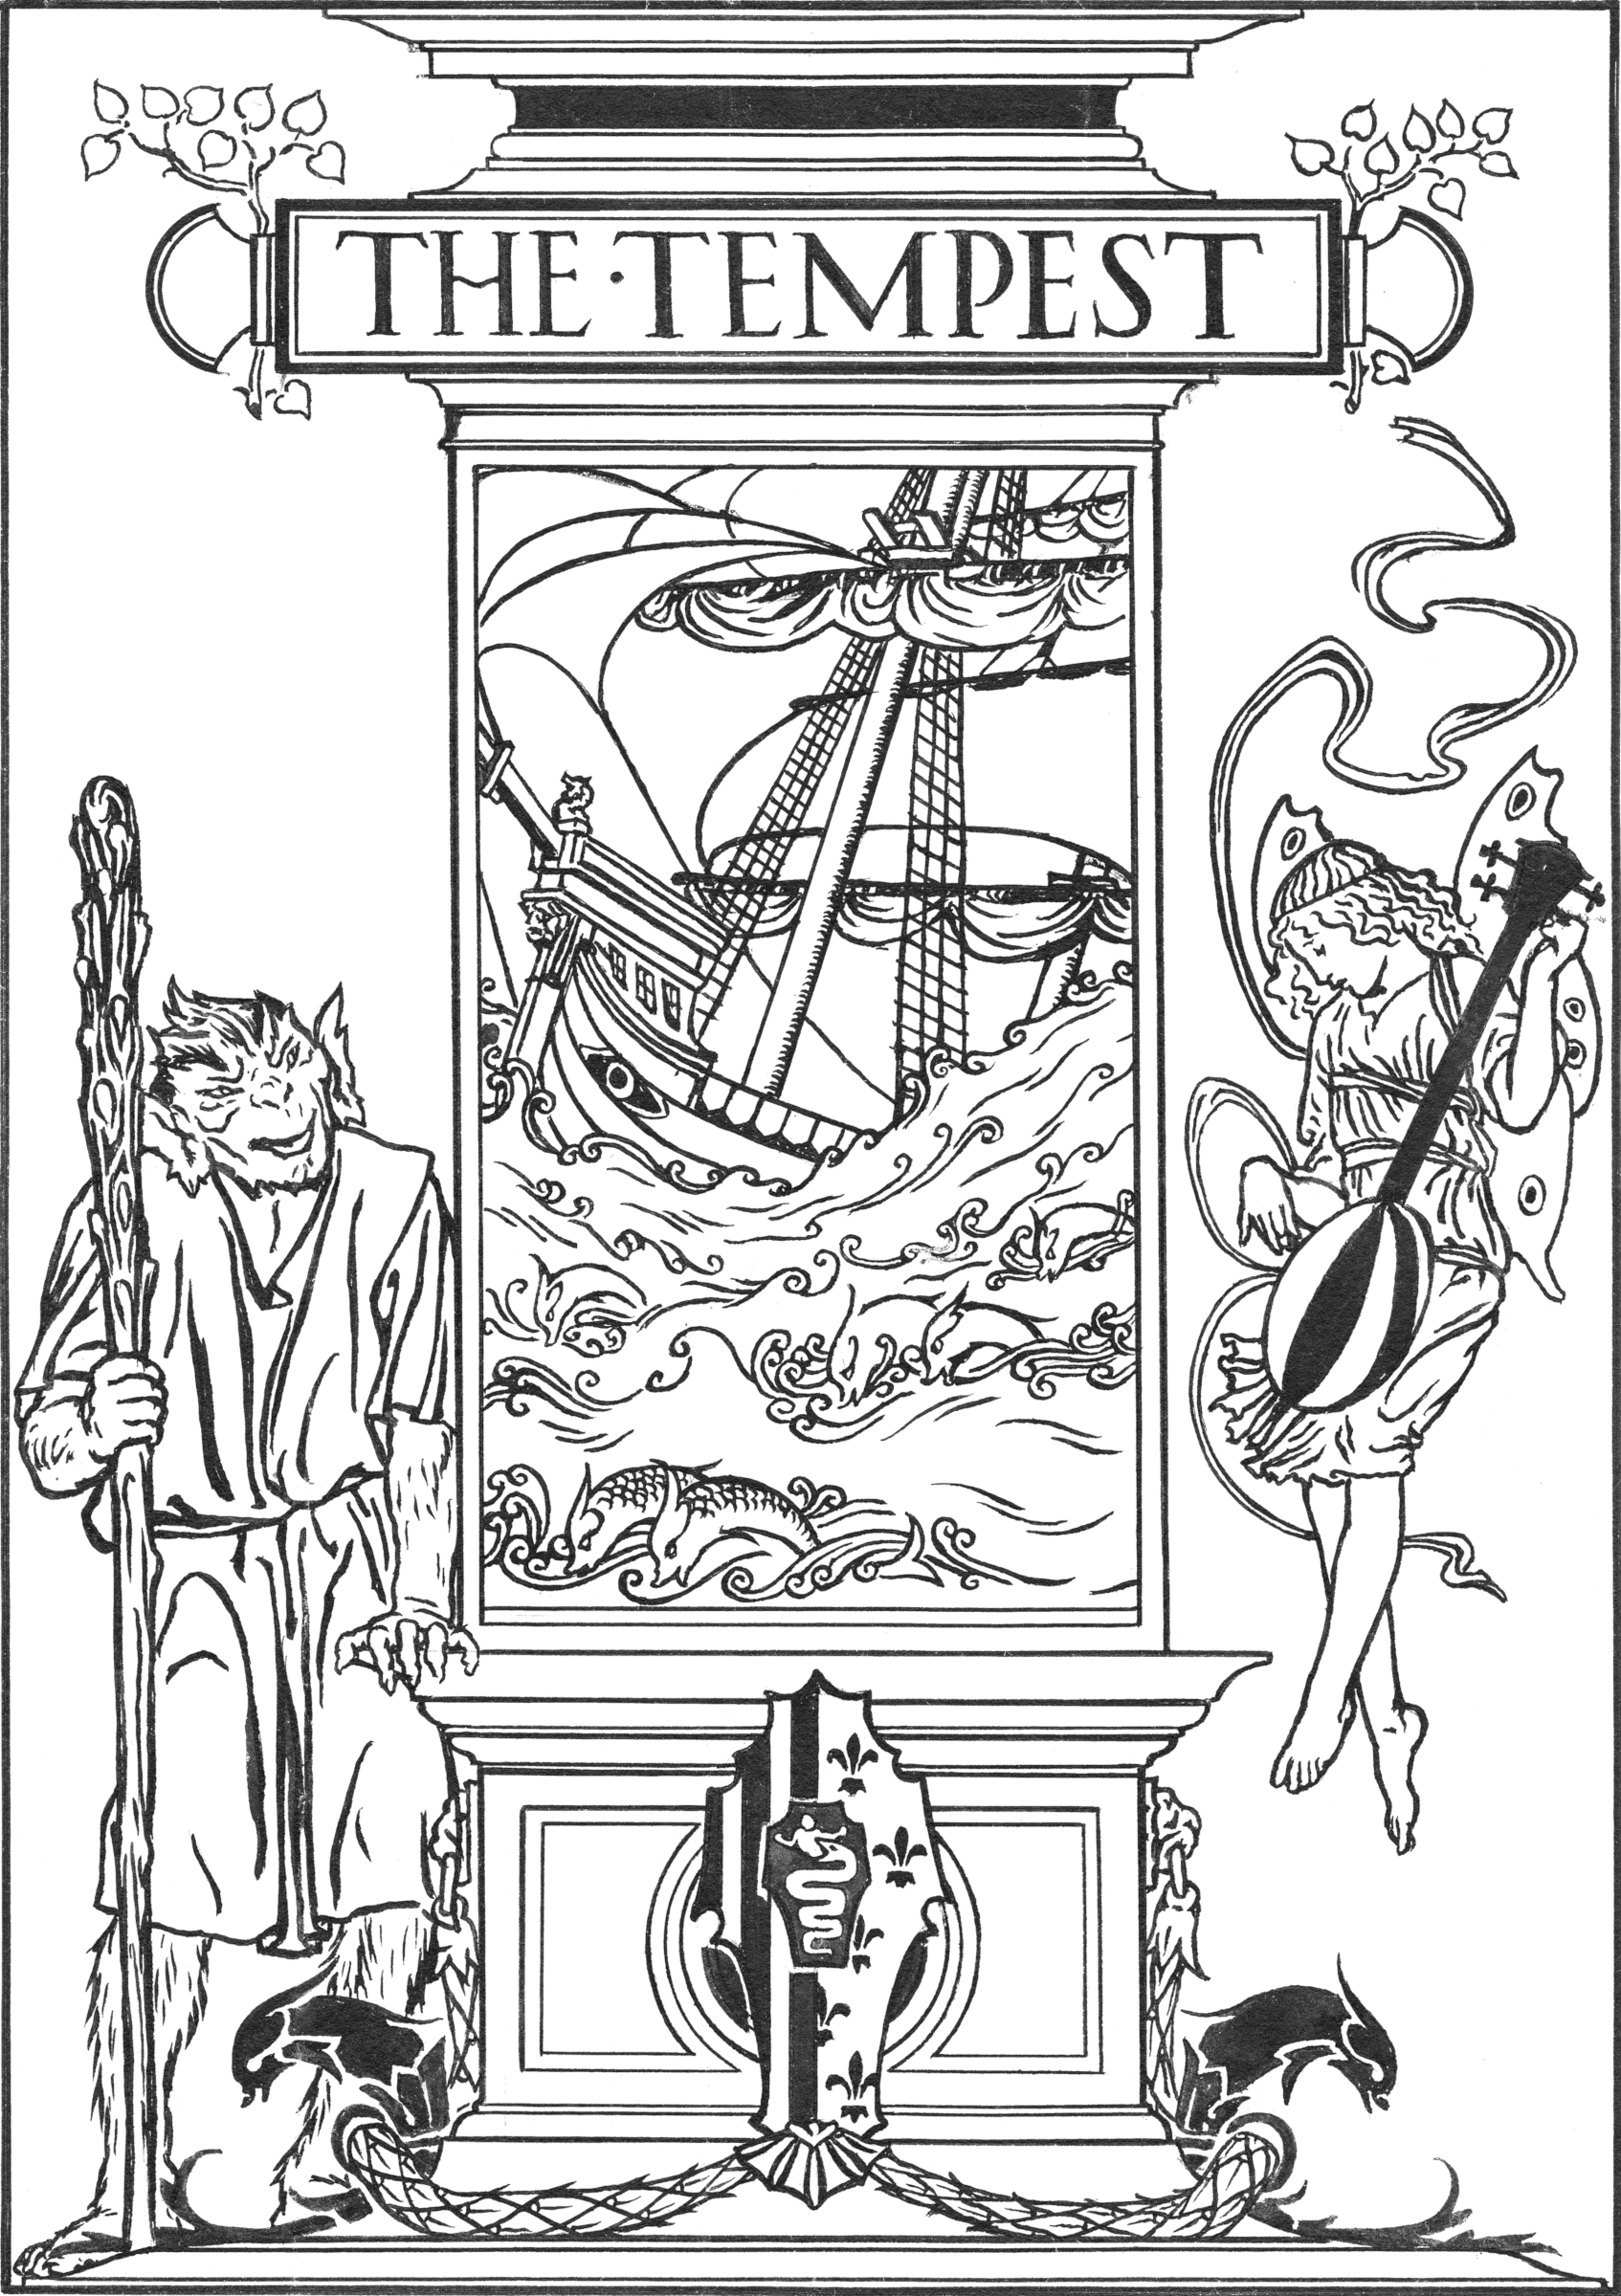
\includepdf[width=1.1\textwidth]{images/cover.jpg}
		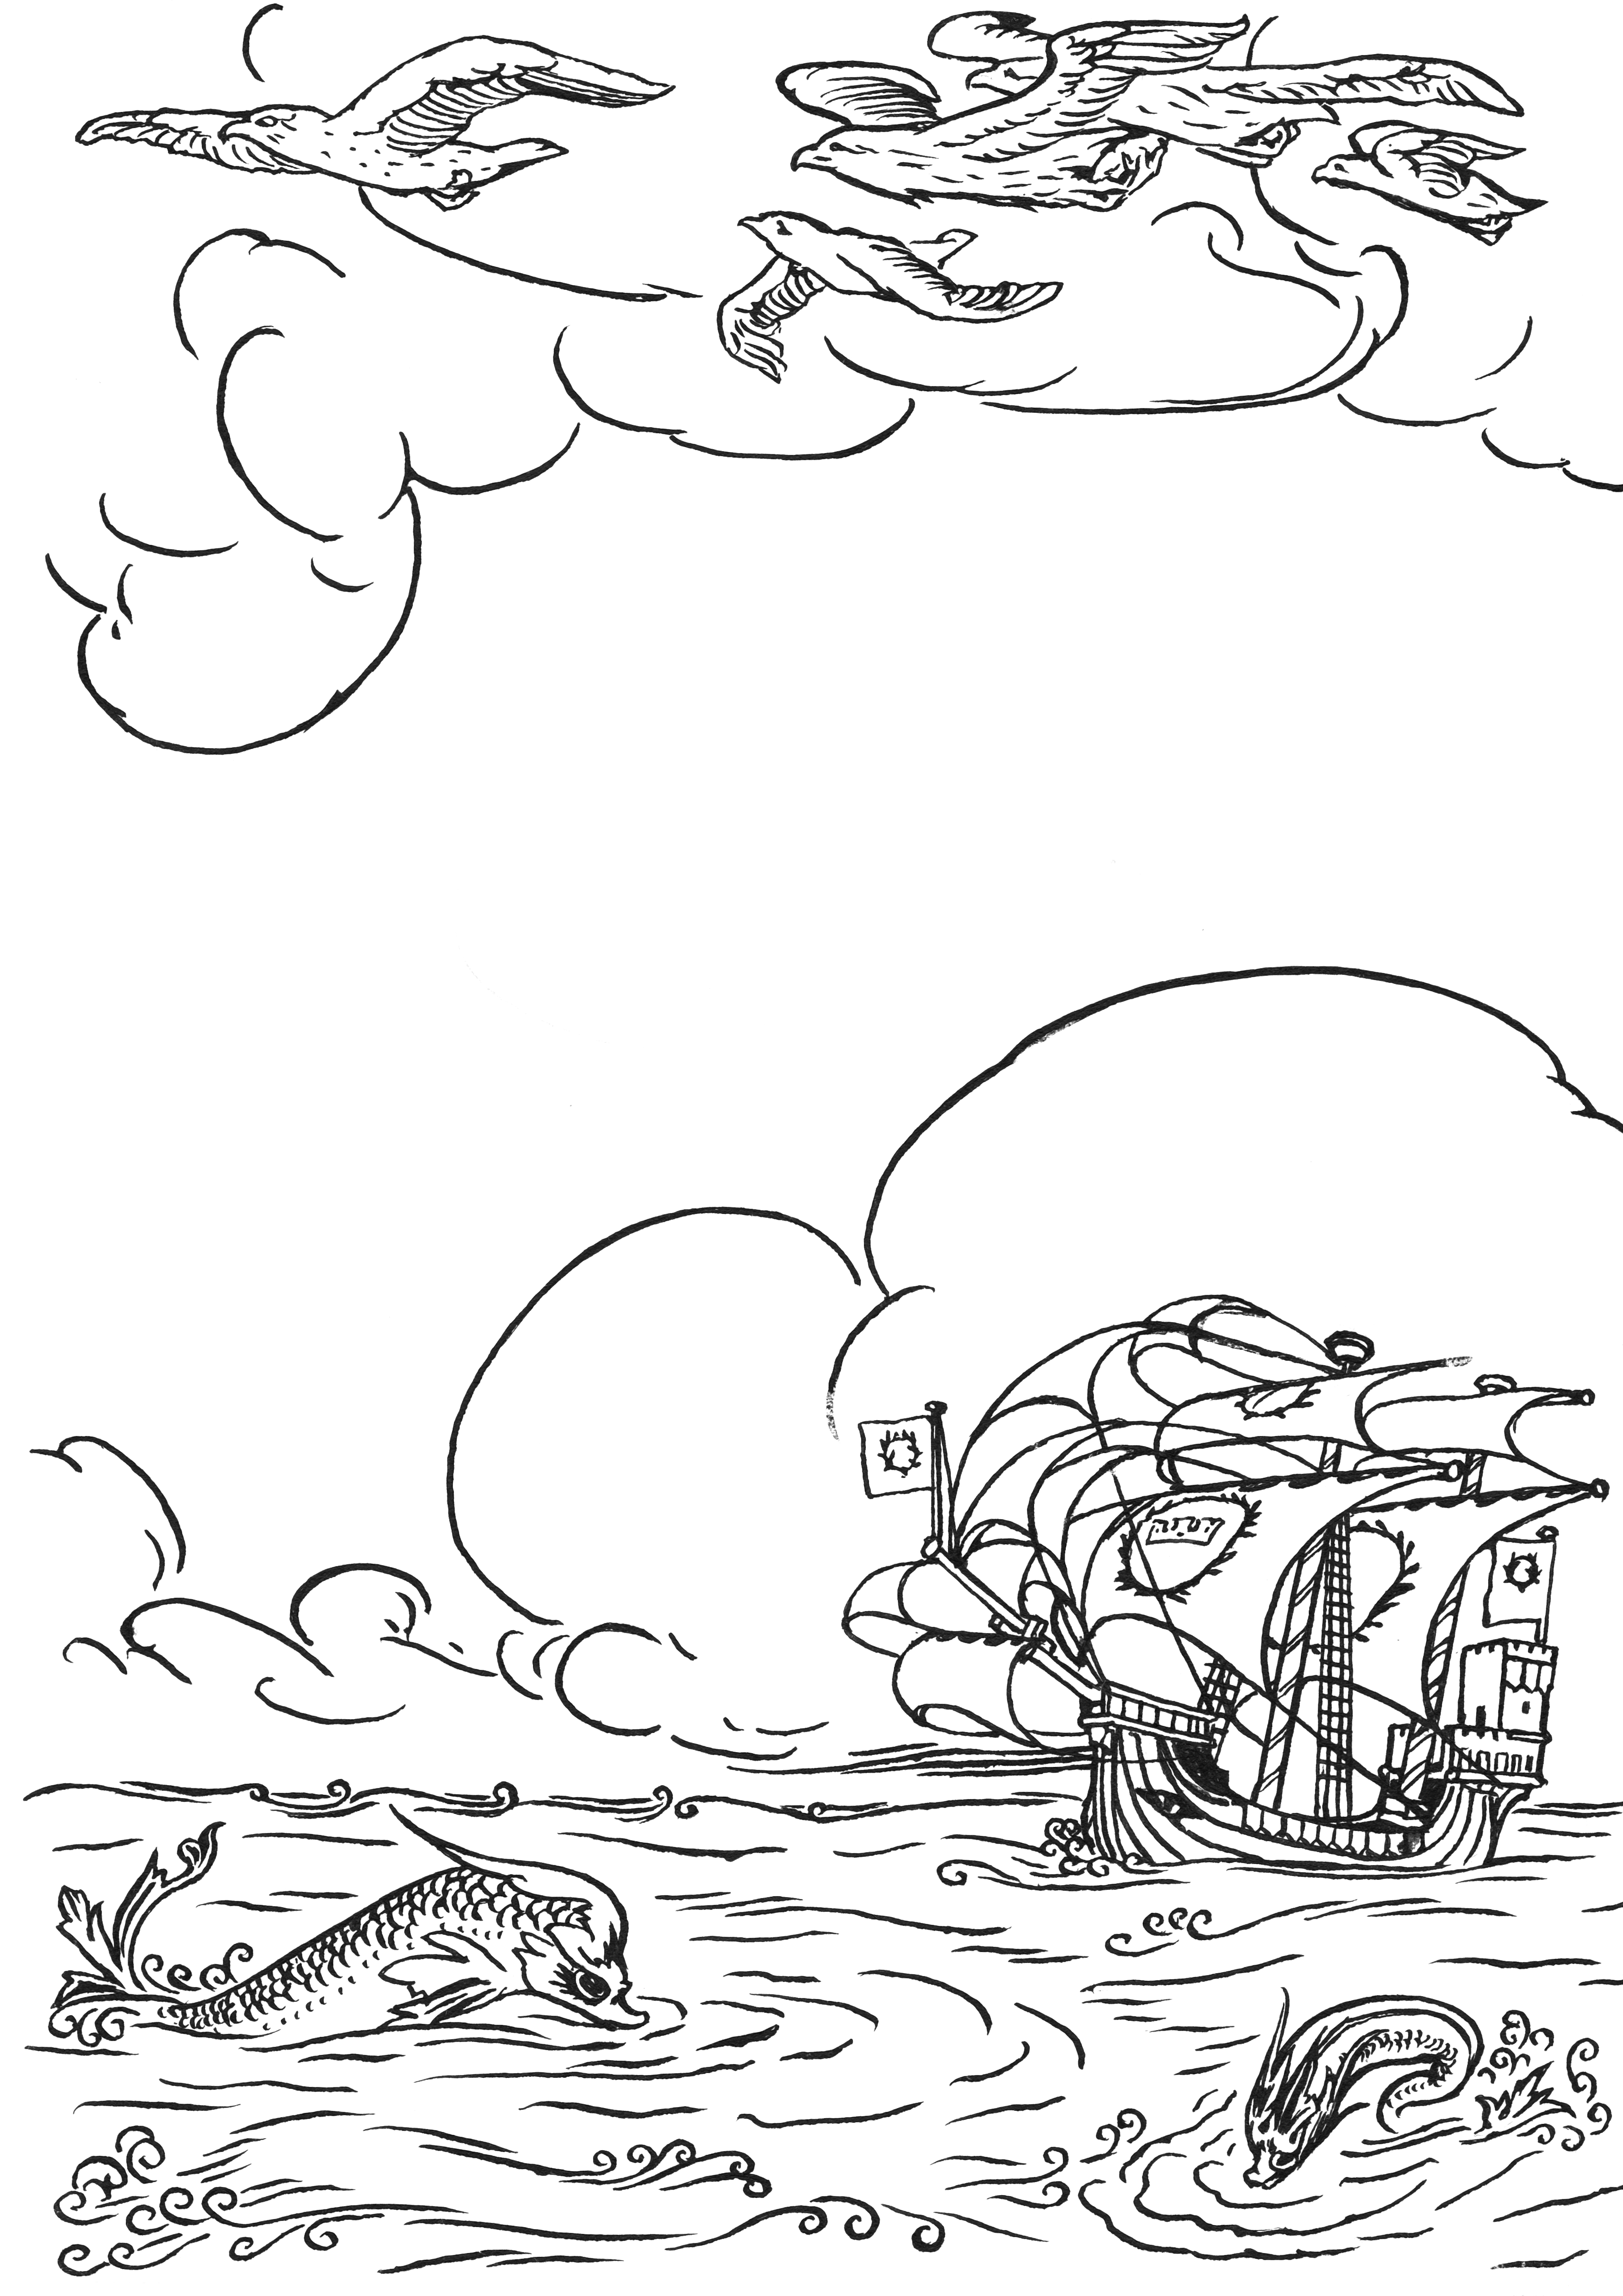
\includepdf[width=1.1\textwidth]{images/endpaper2.jpg}
		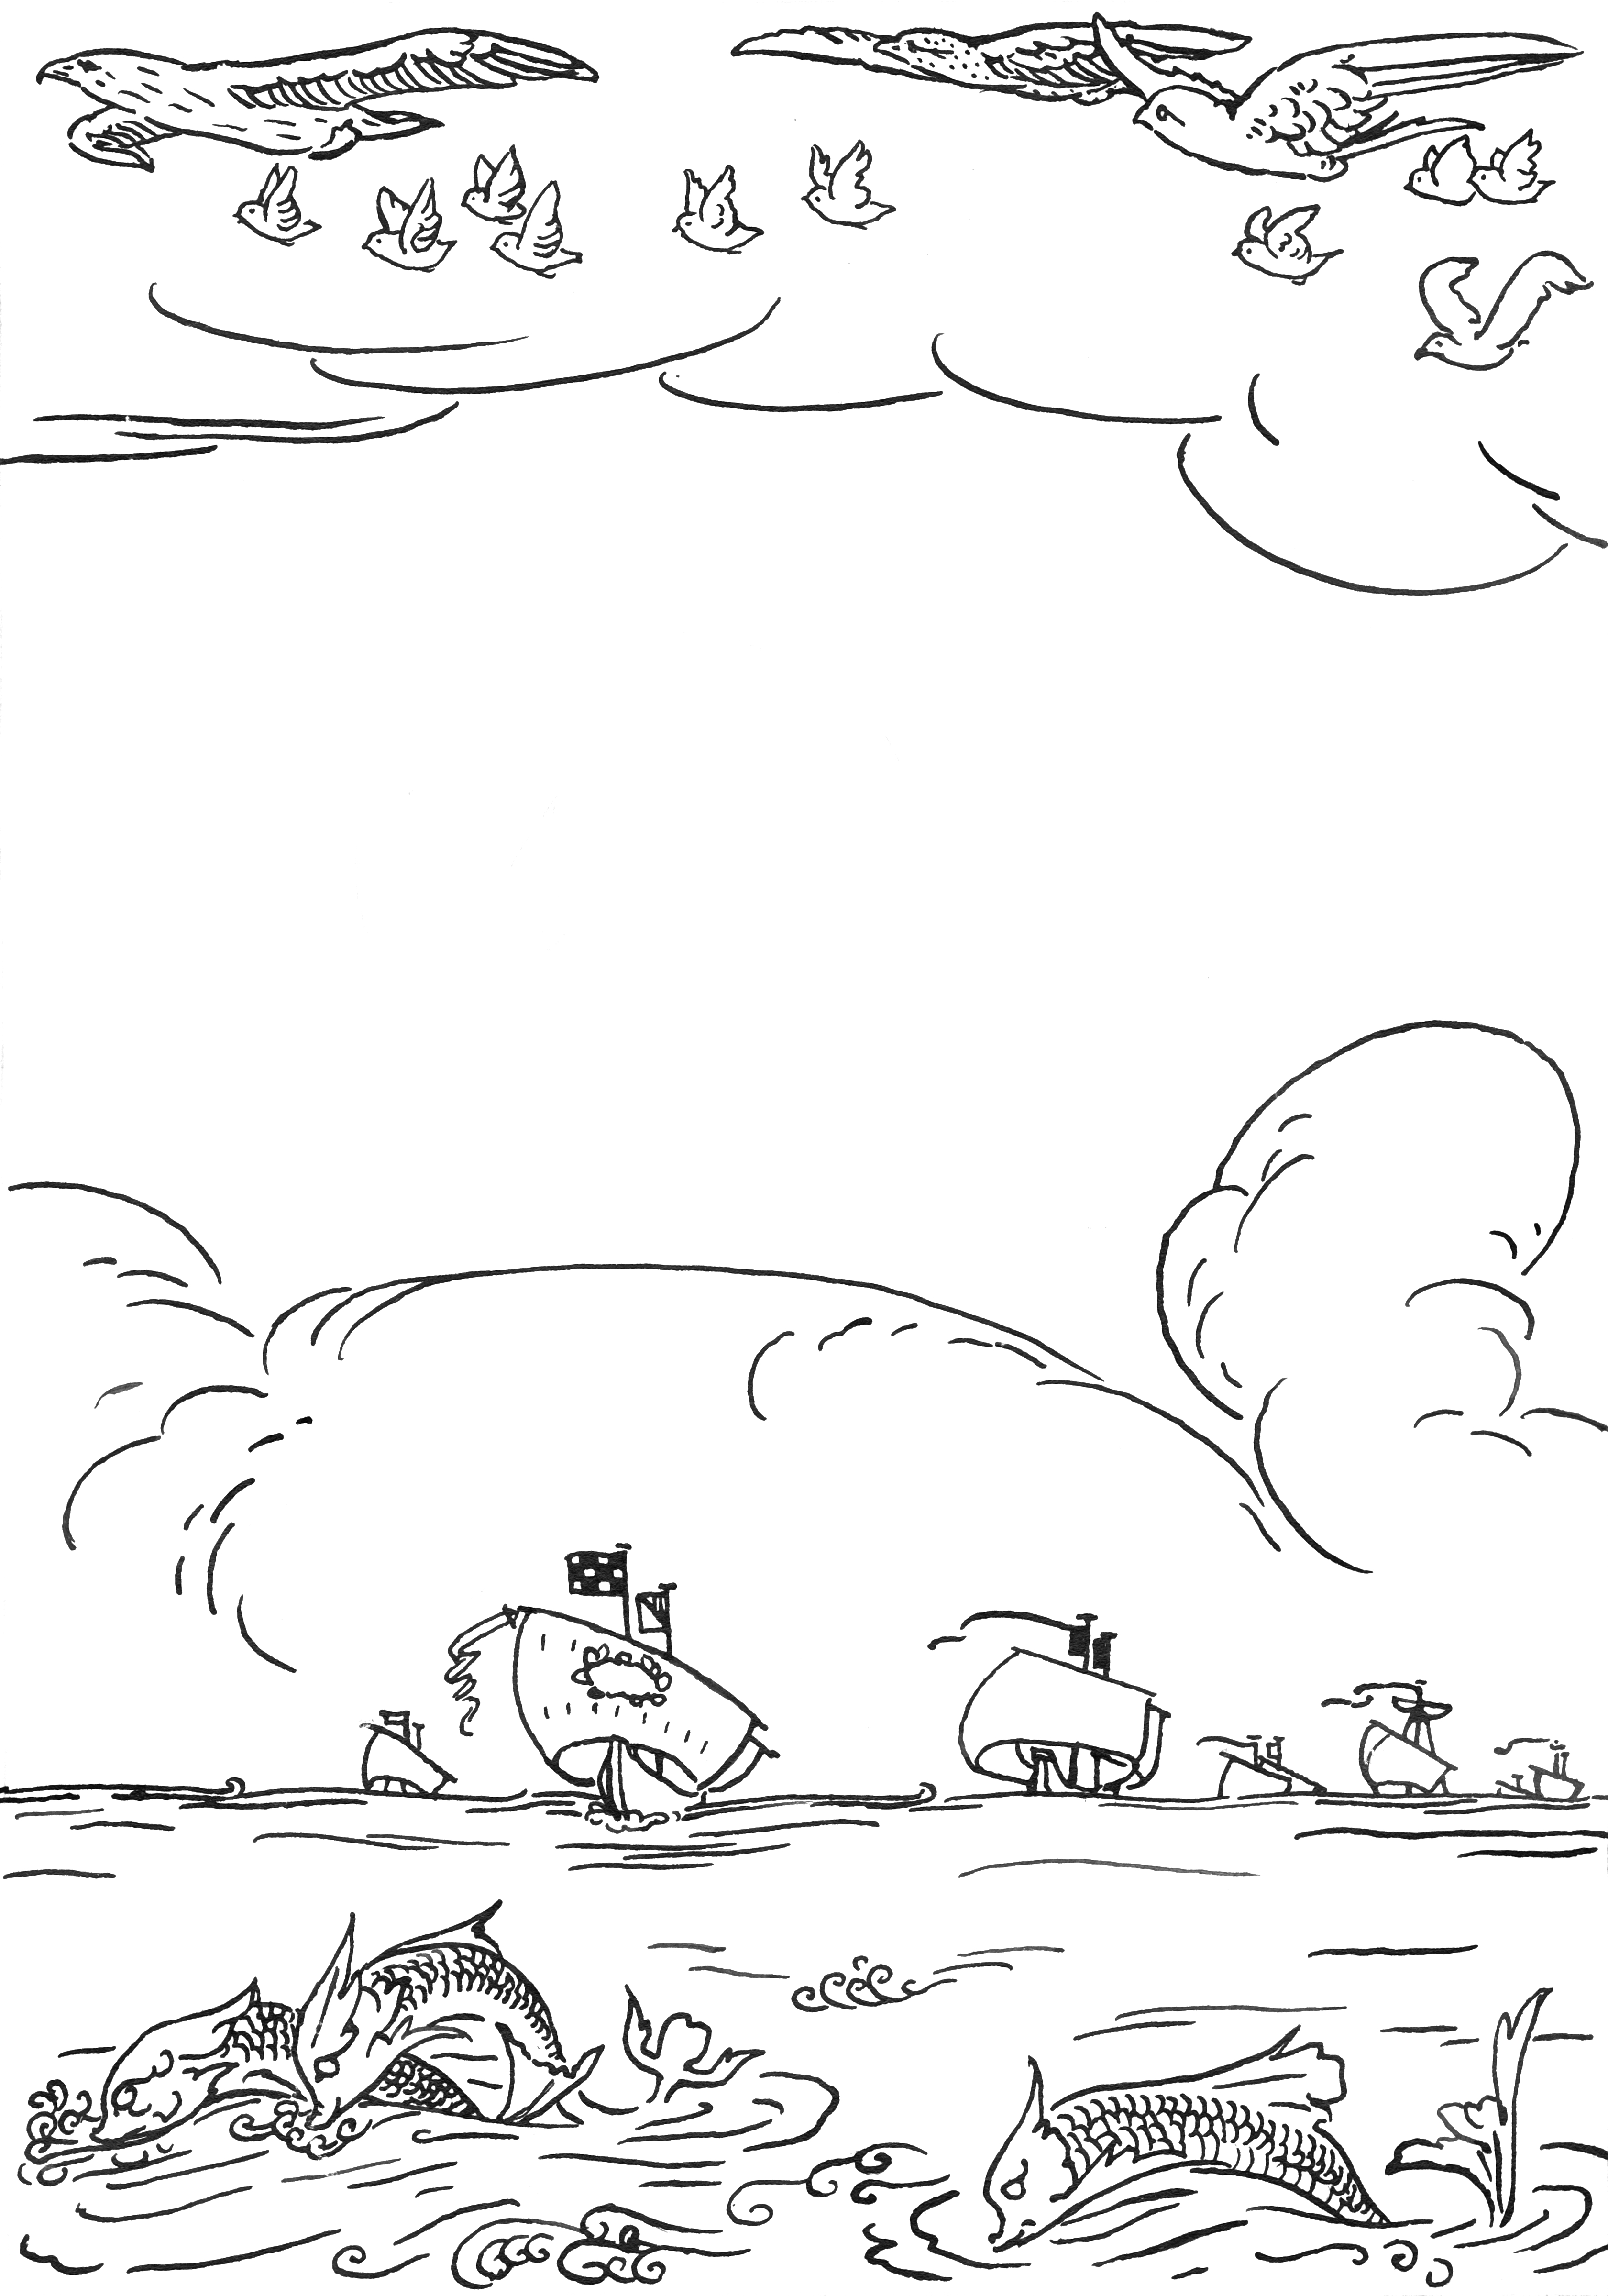
\includepdf[width=1.1\textwidth]{images/endpaper1.jpg}
		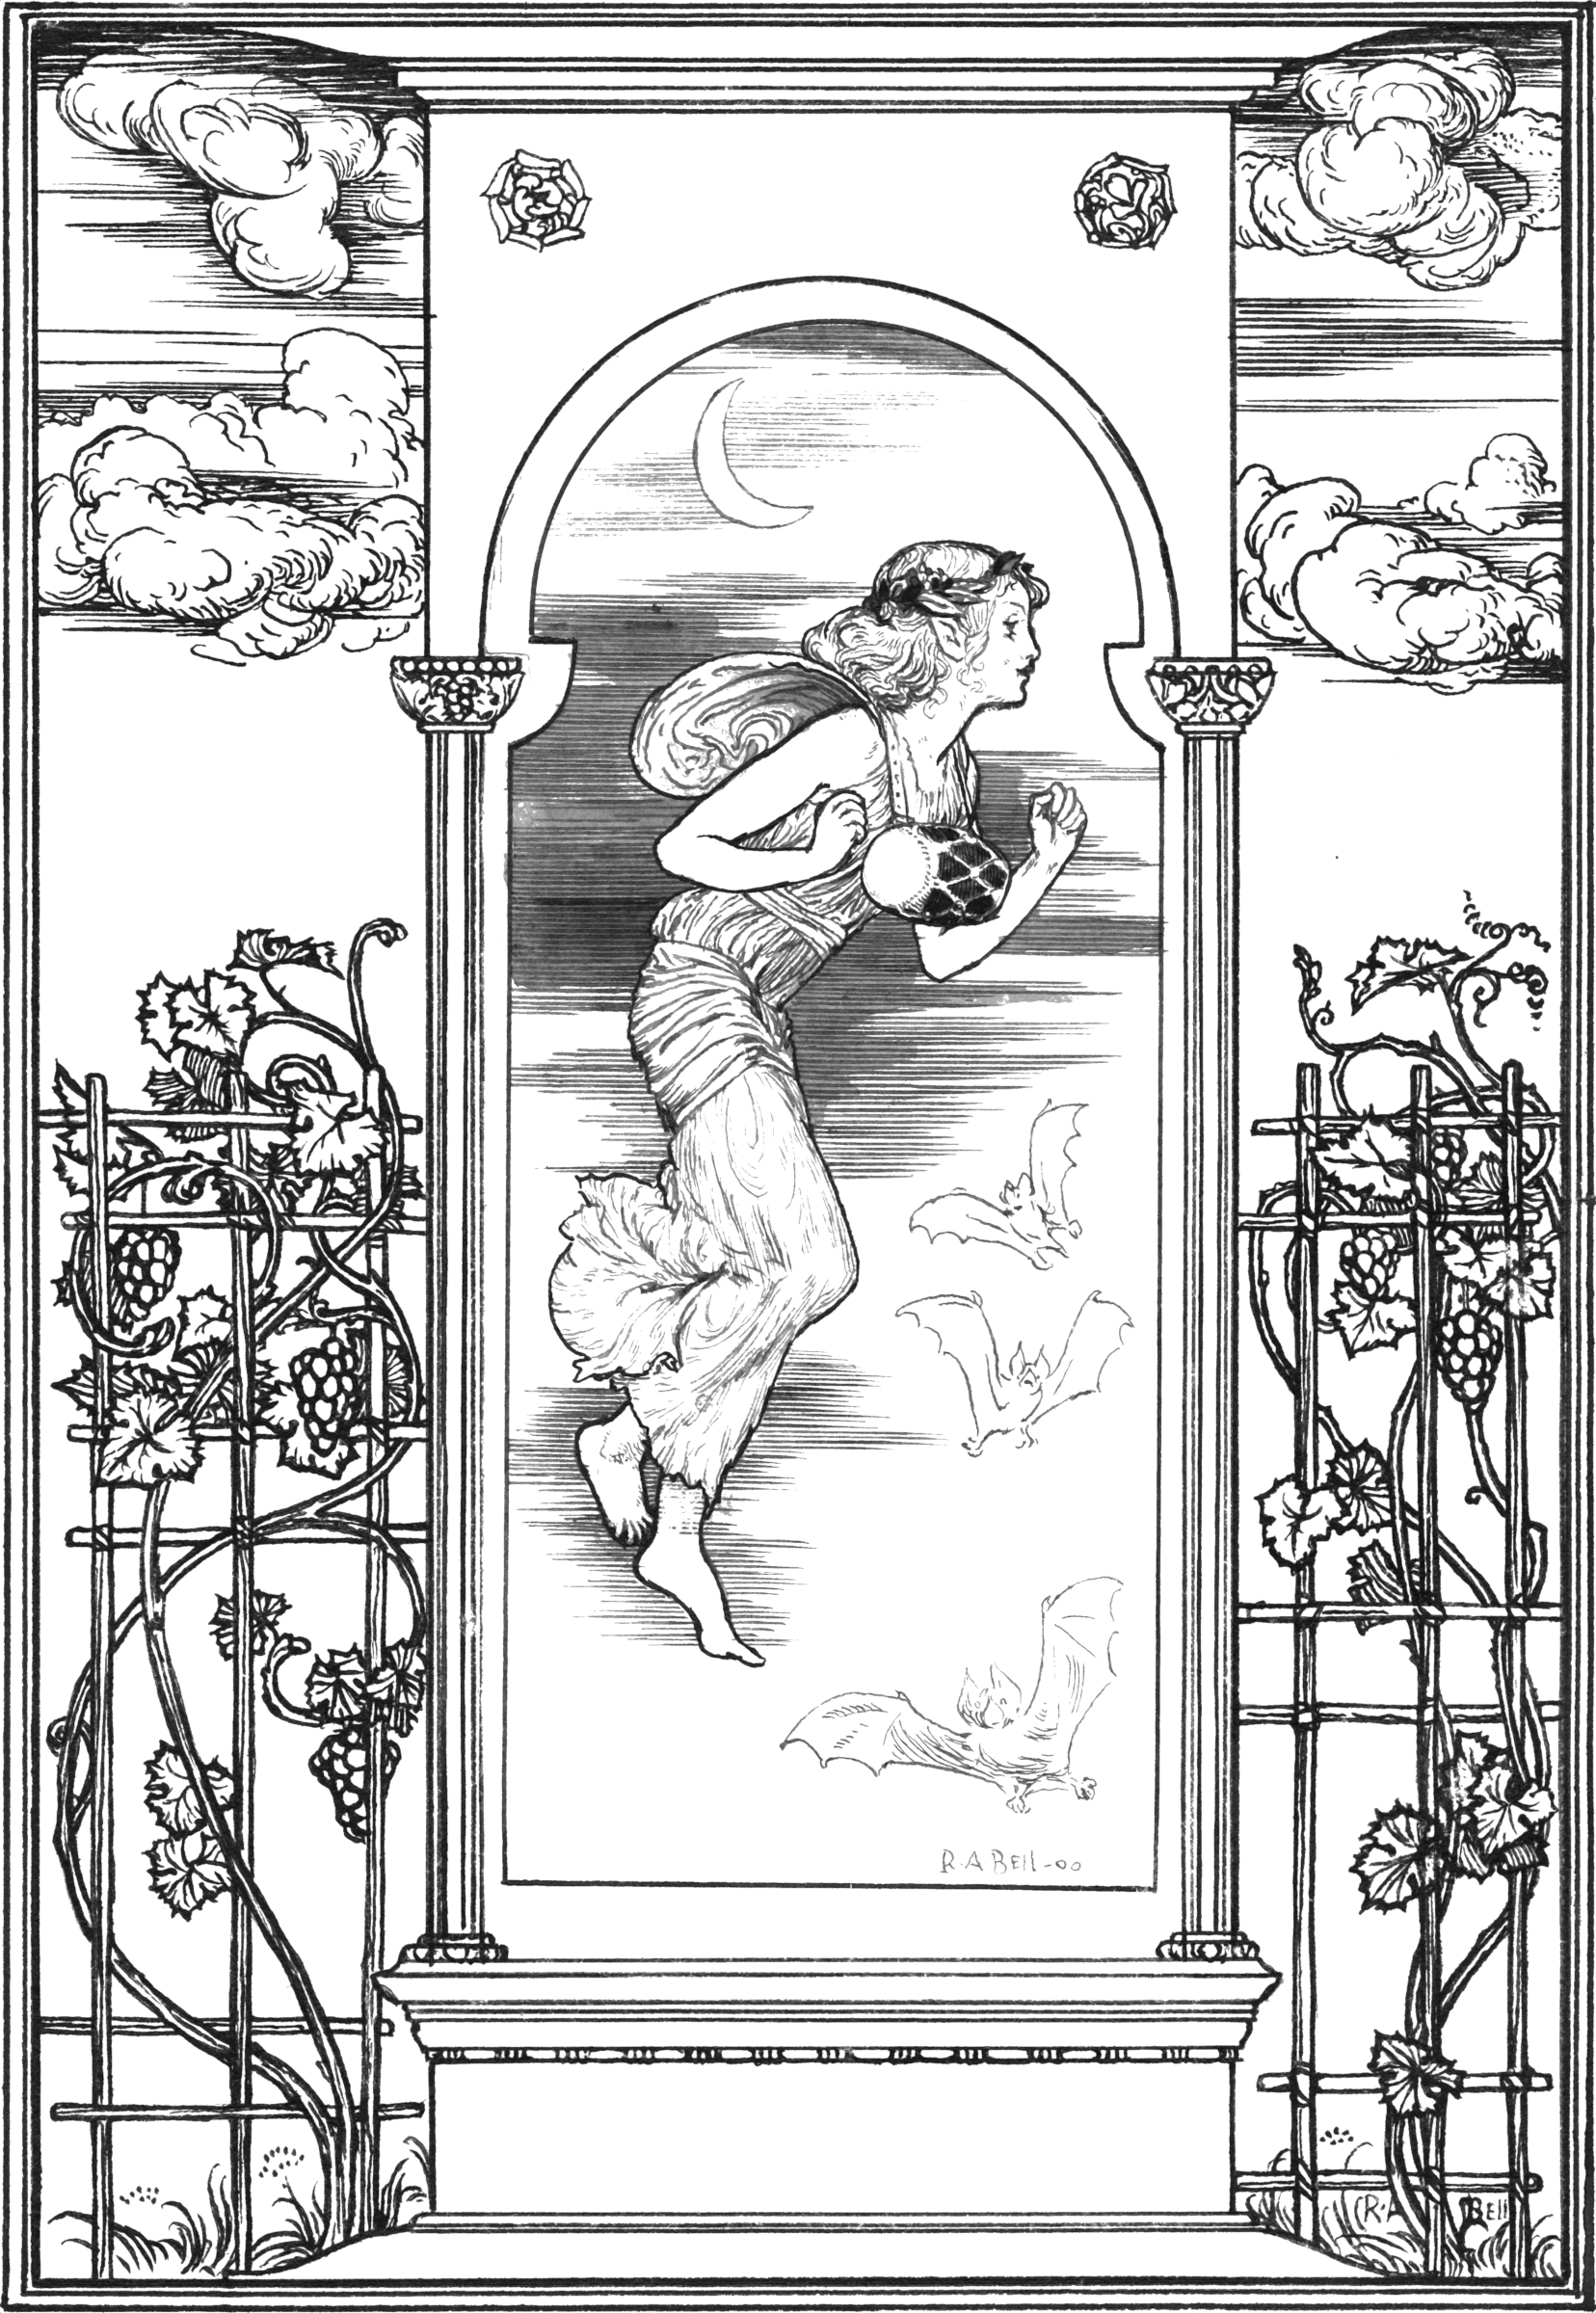
\includepdf[width=1.1\textwidth]{images/arielbat.jpg}
		
\includepdf[width=1.1\textwidth]{images/archpage.jpg}
		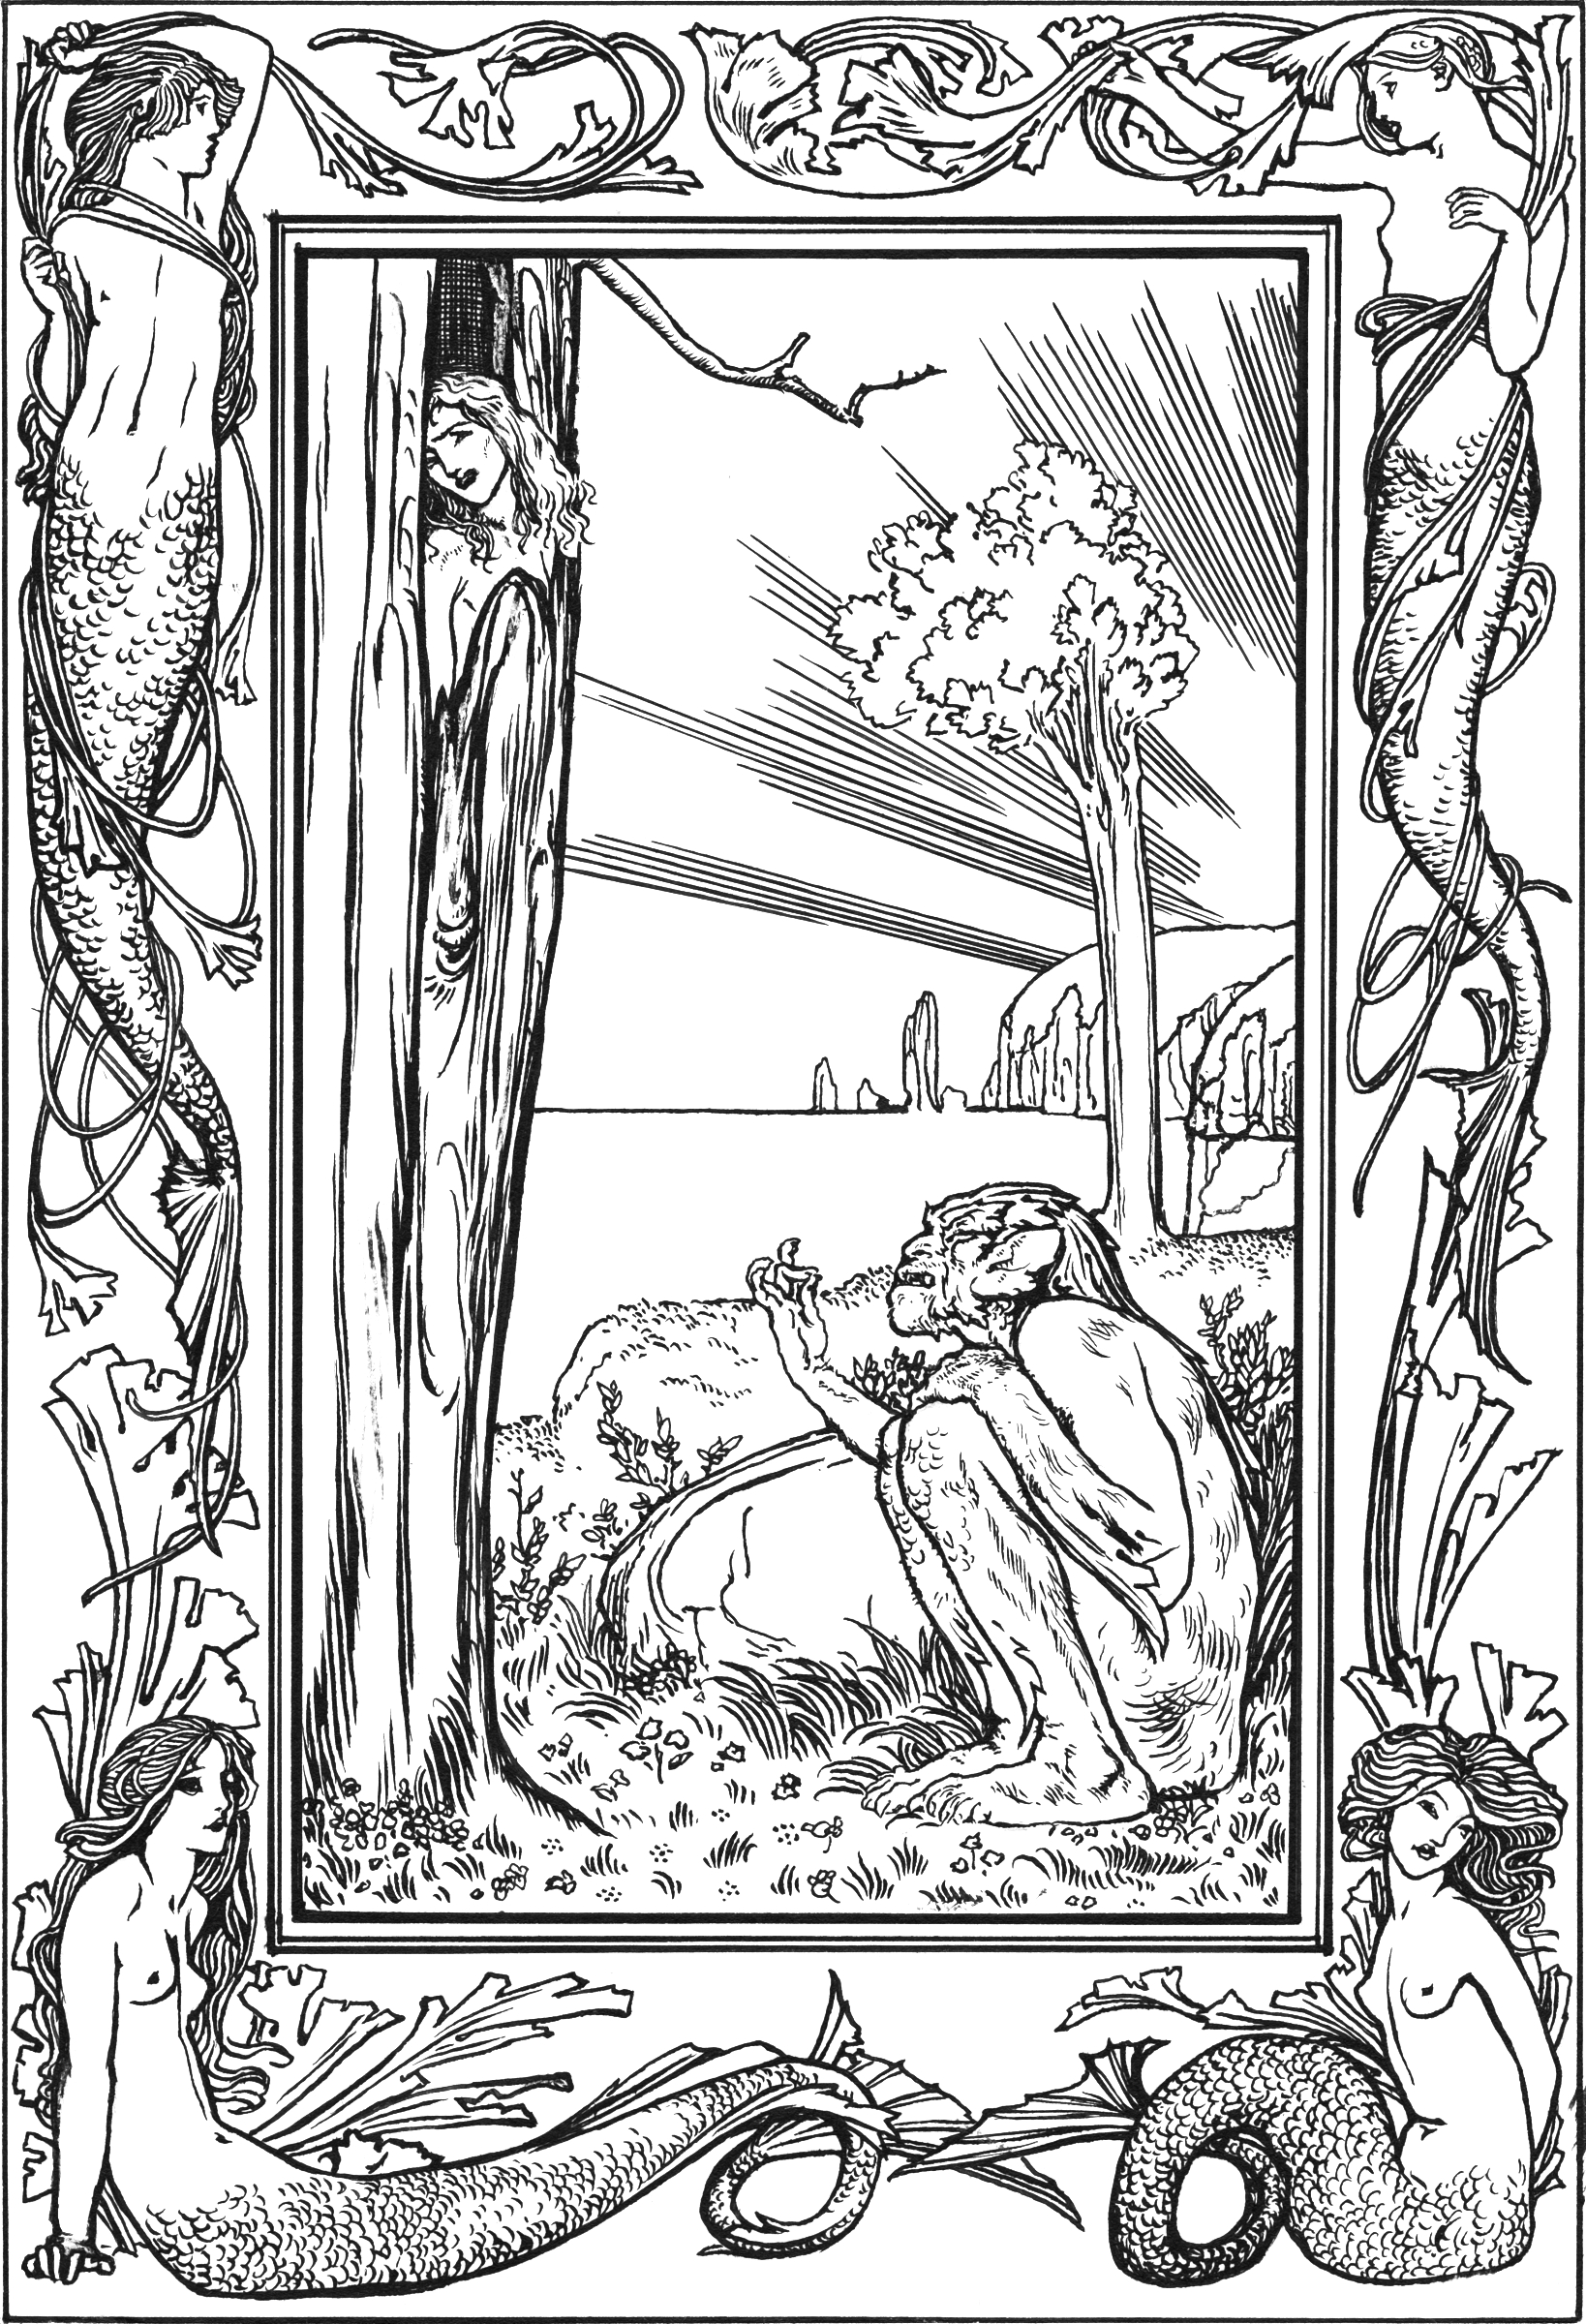
\includepdf[width=1.1\textwidth]{images/clovenpine.jpg}
		\tableofcontents
		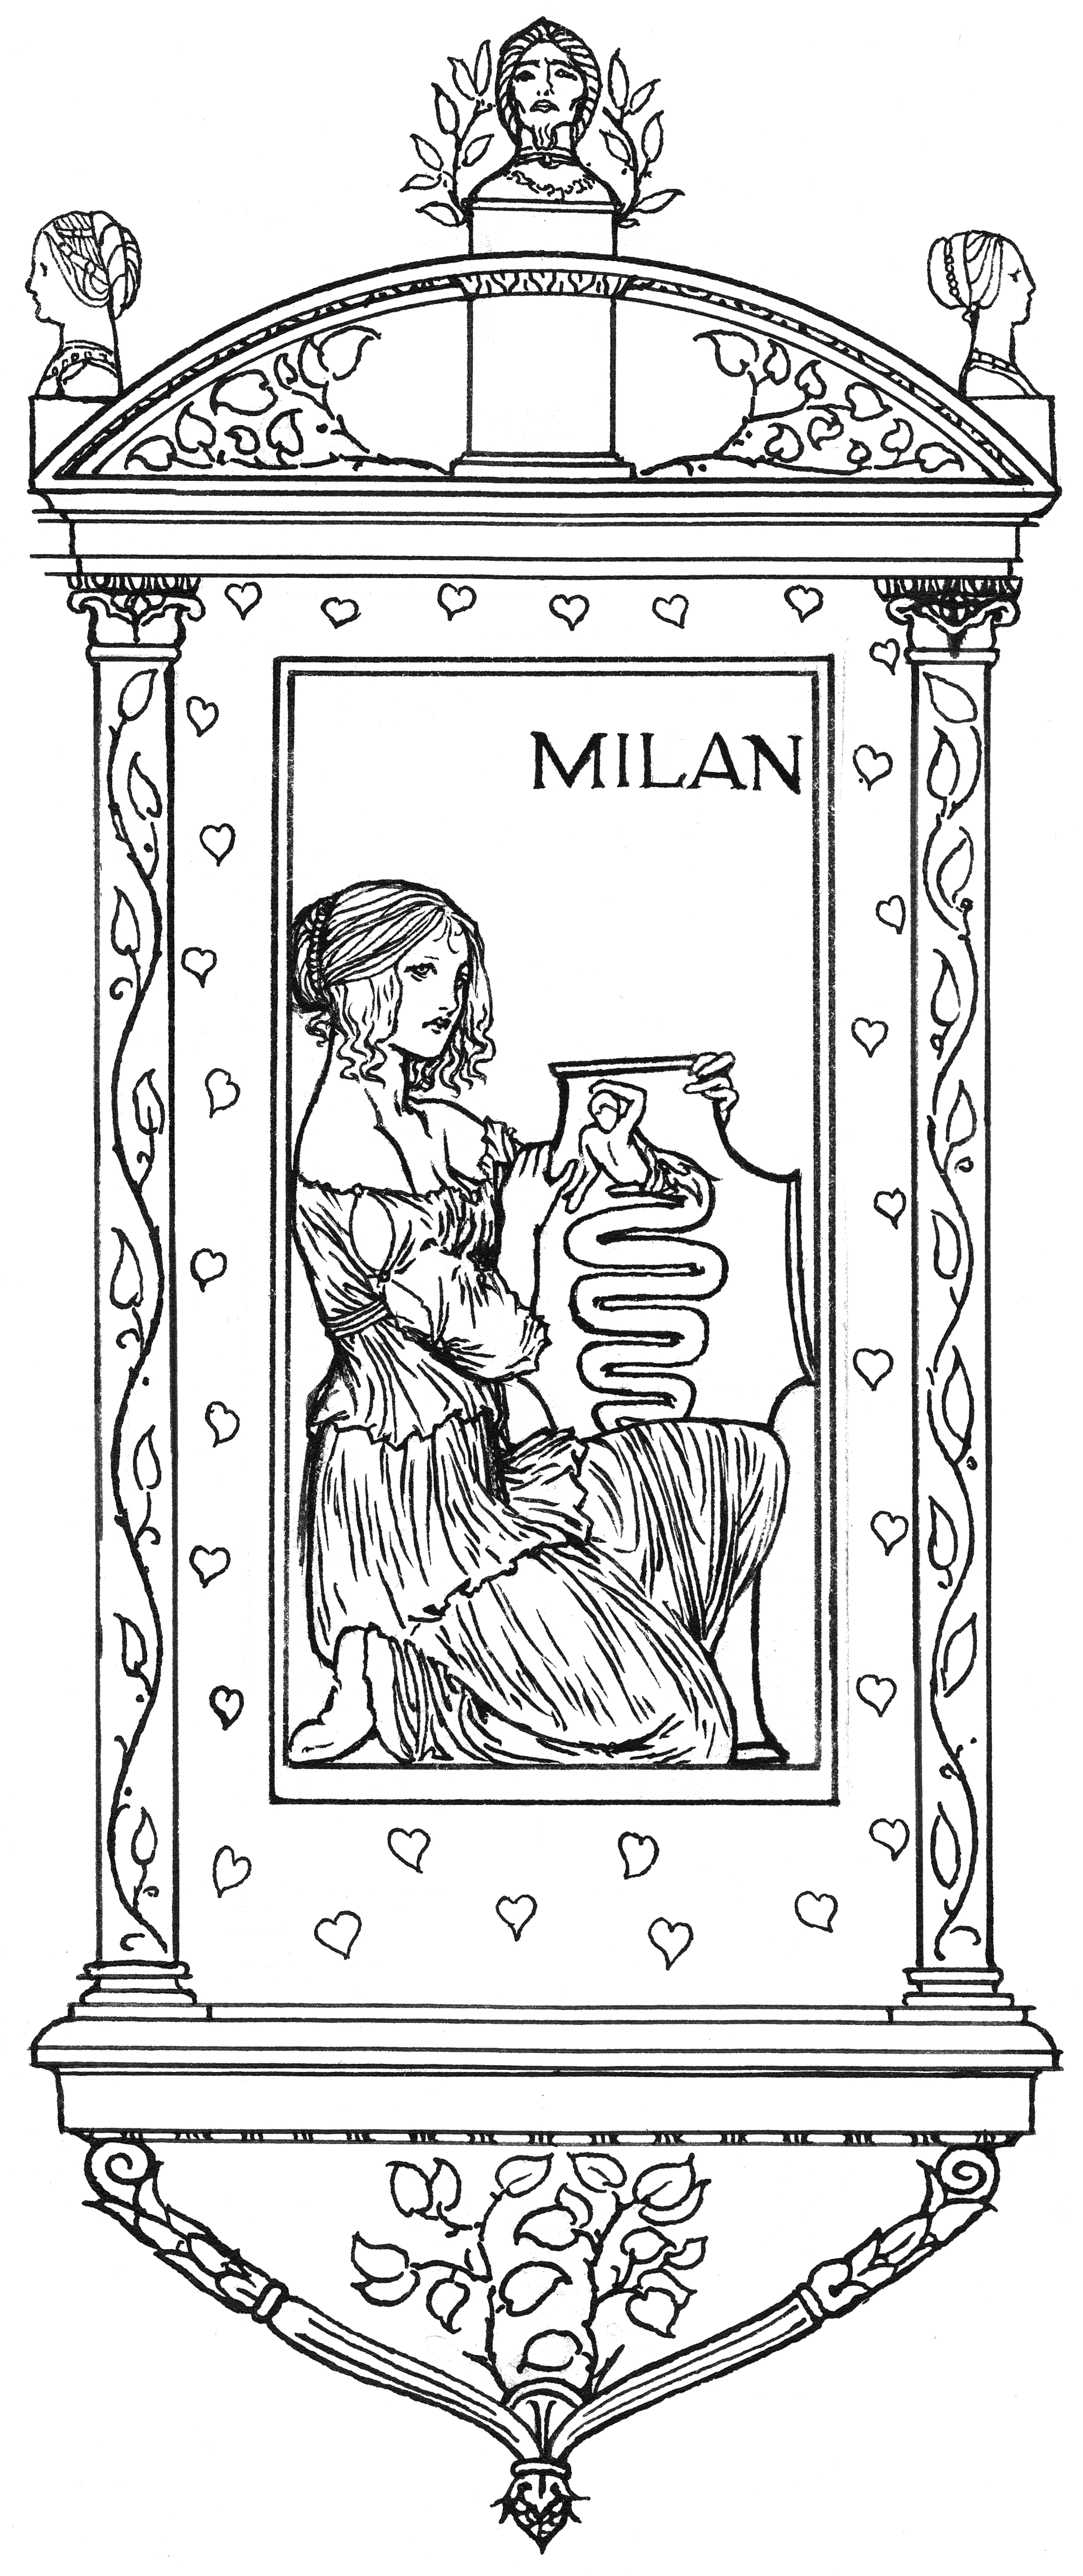
\includepdf[width=.7\textwidth]{images/milan.jpg}
		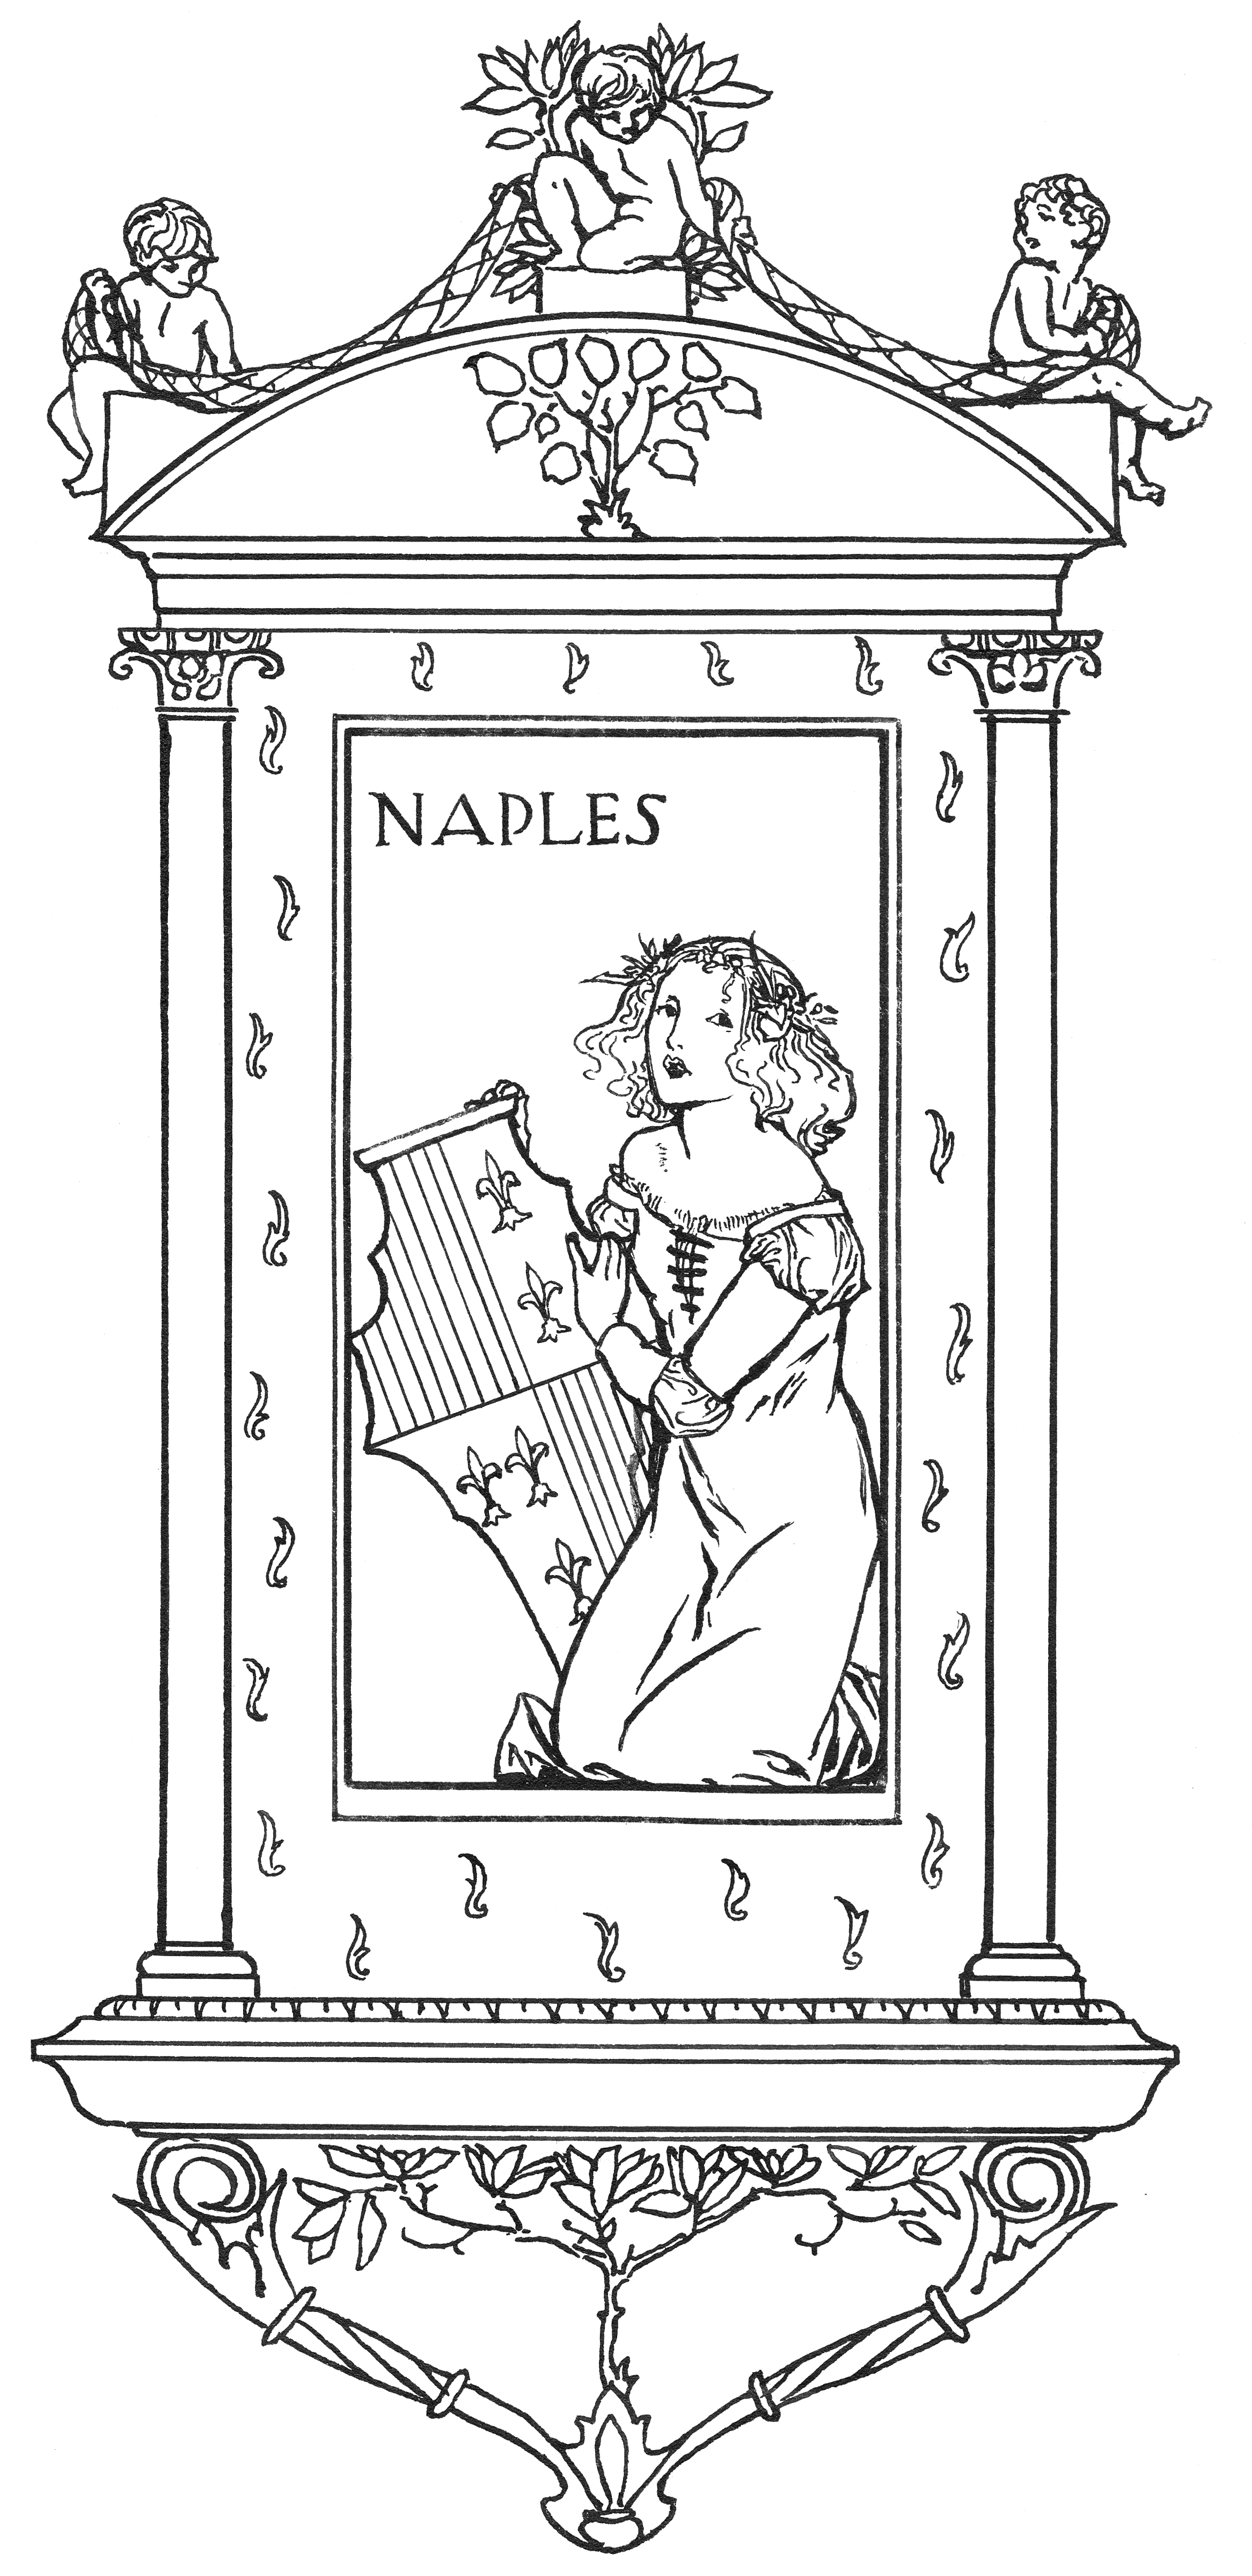
\includepdf[width=.8\textwidth]{images/naples.jpg}
		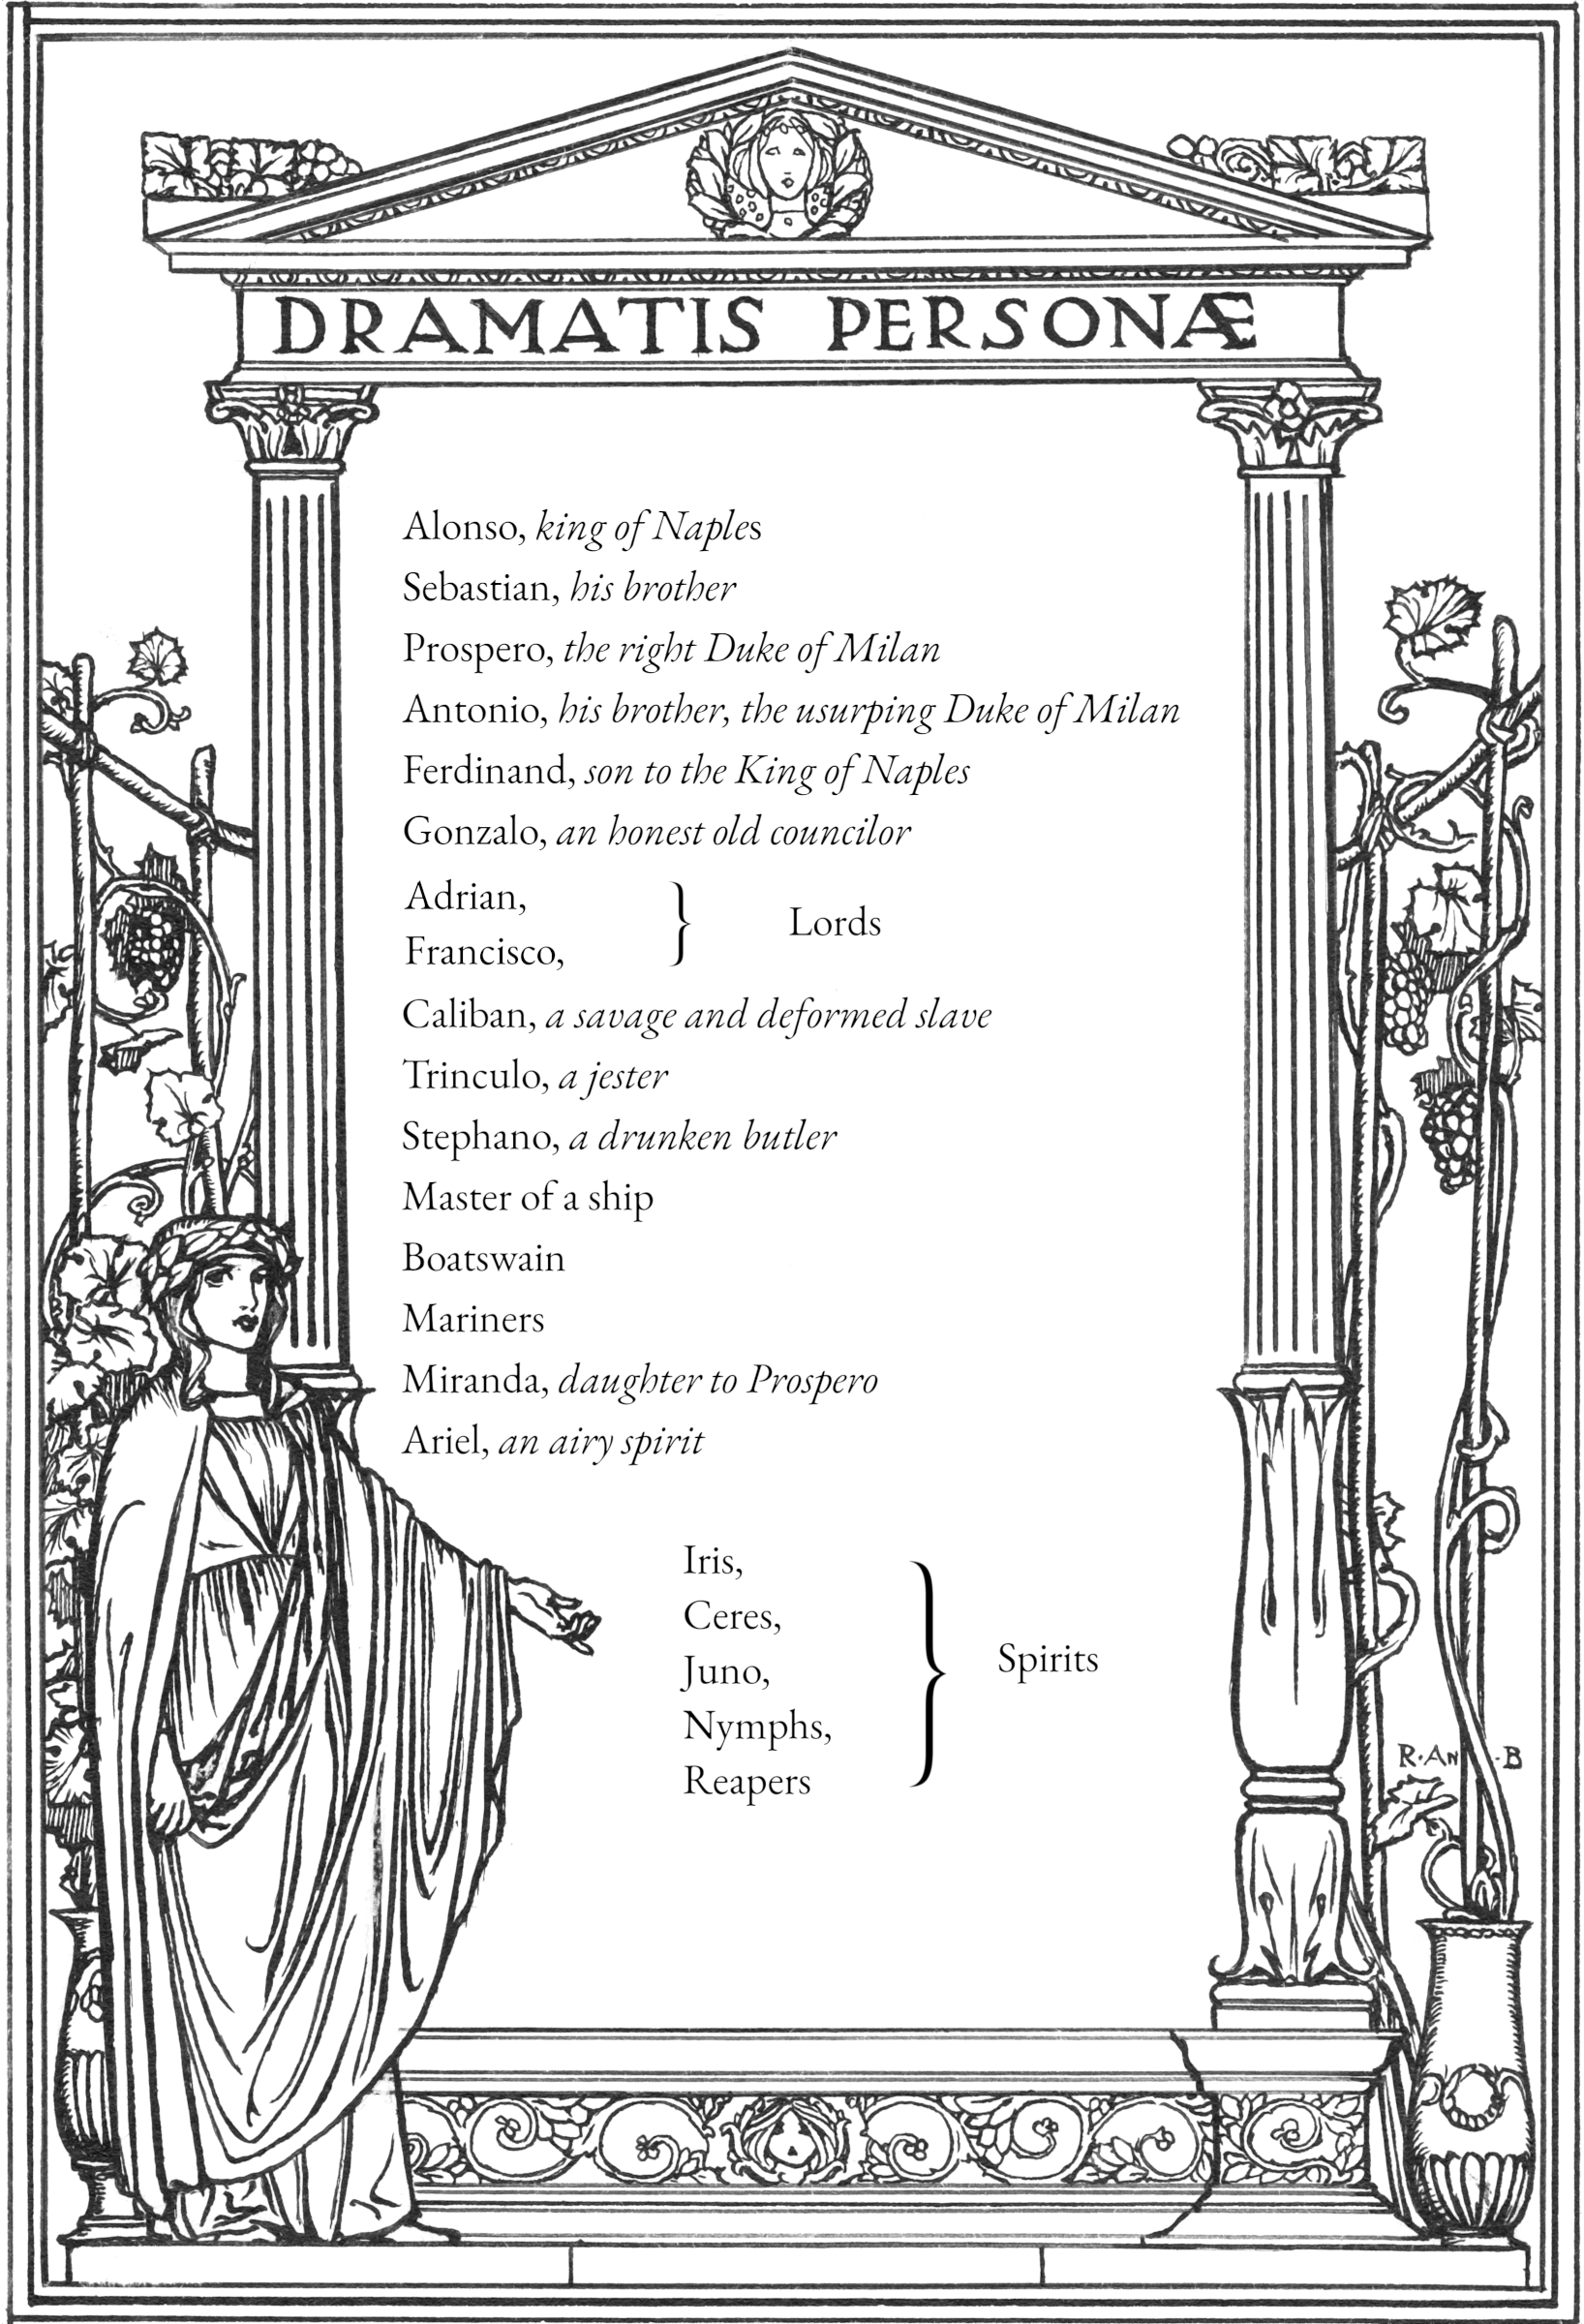
\includepdf[width=1.1\textwidth]{images/dramper.jpg}
	\end{letter}
	\begin{a4}
		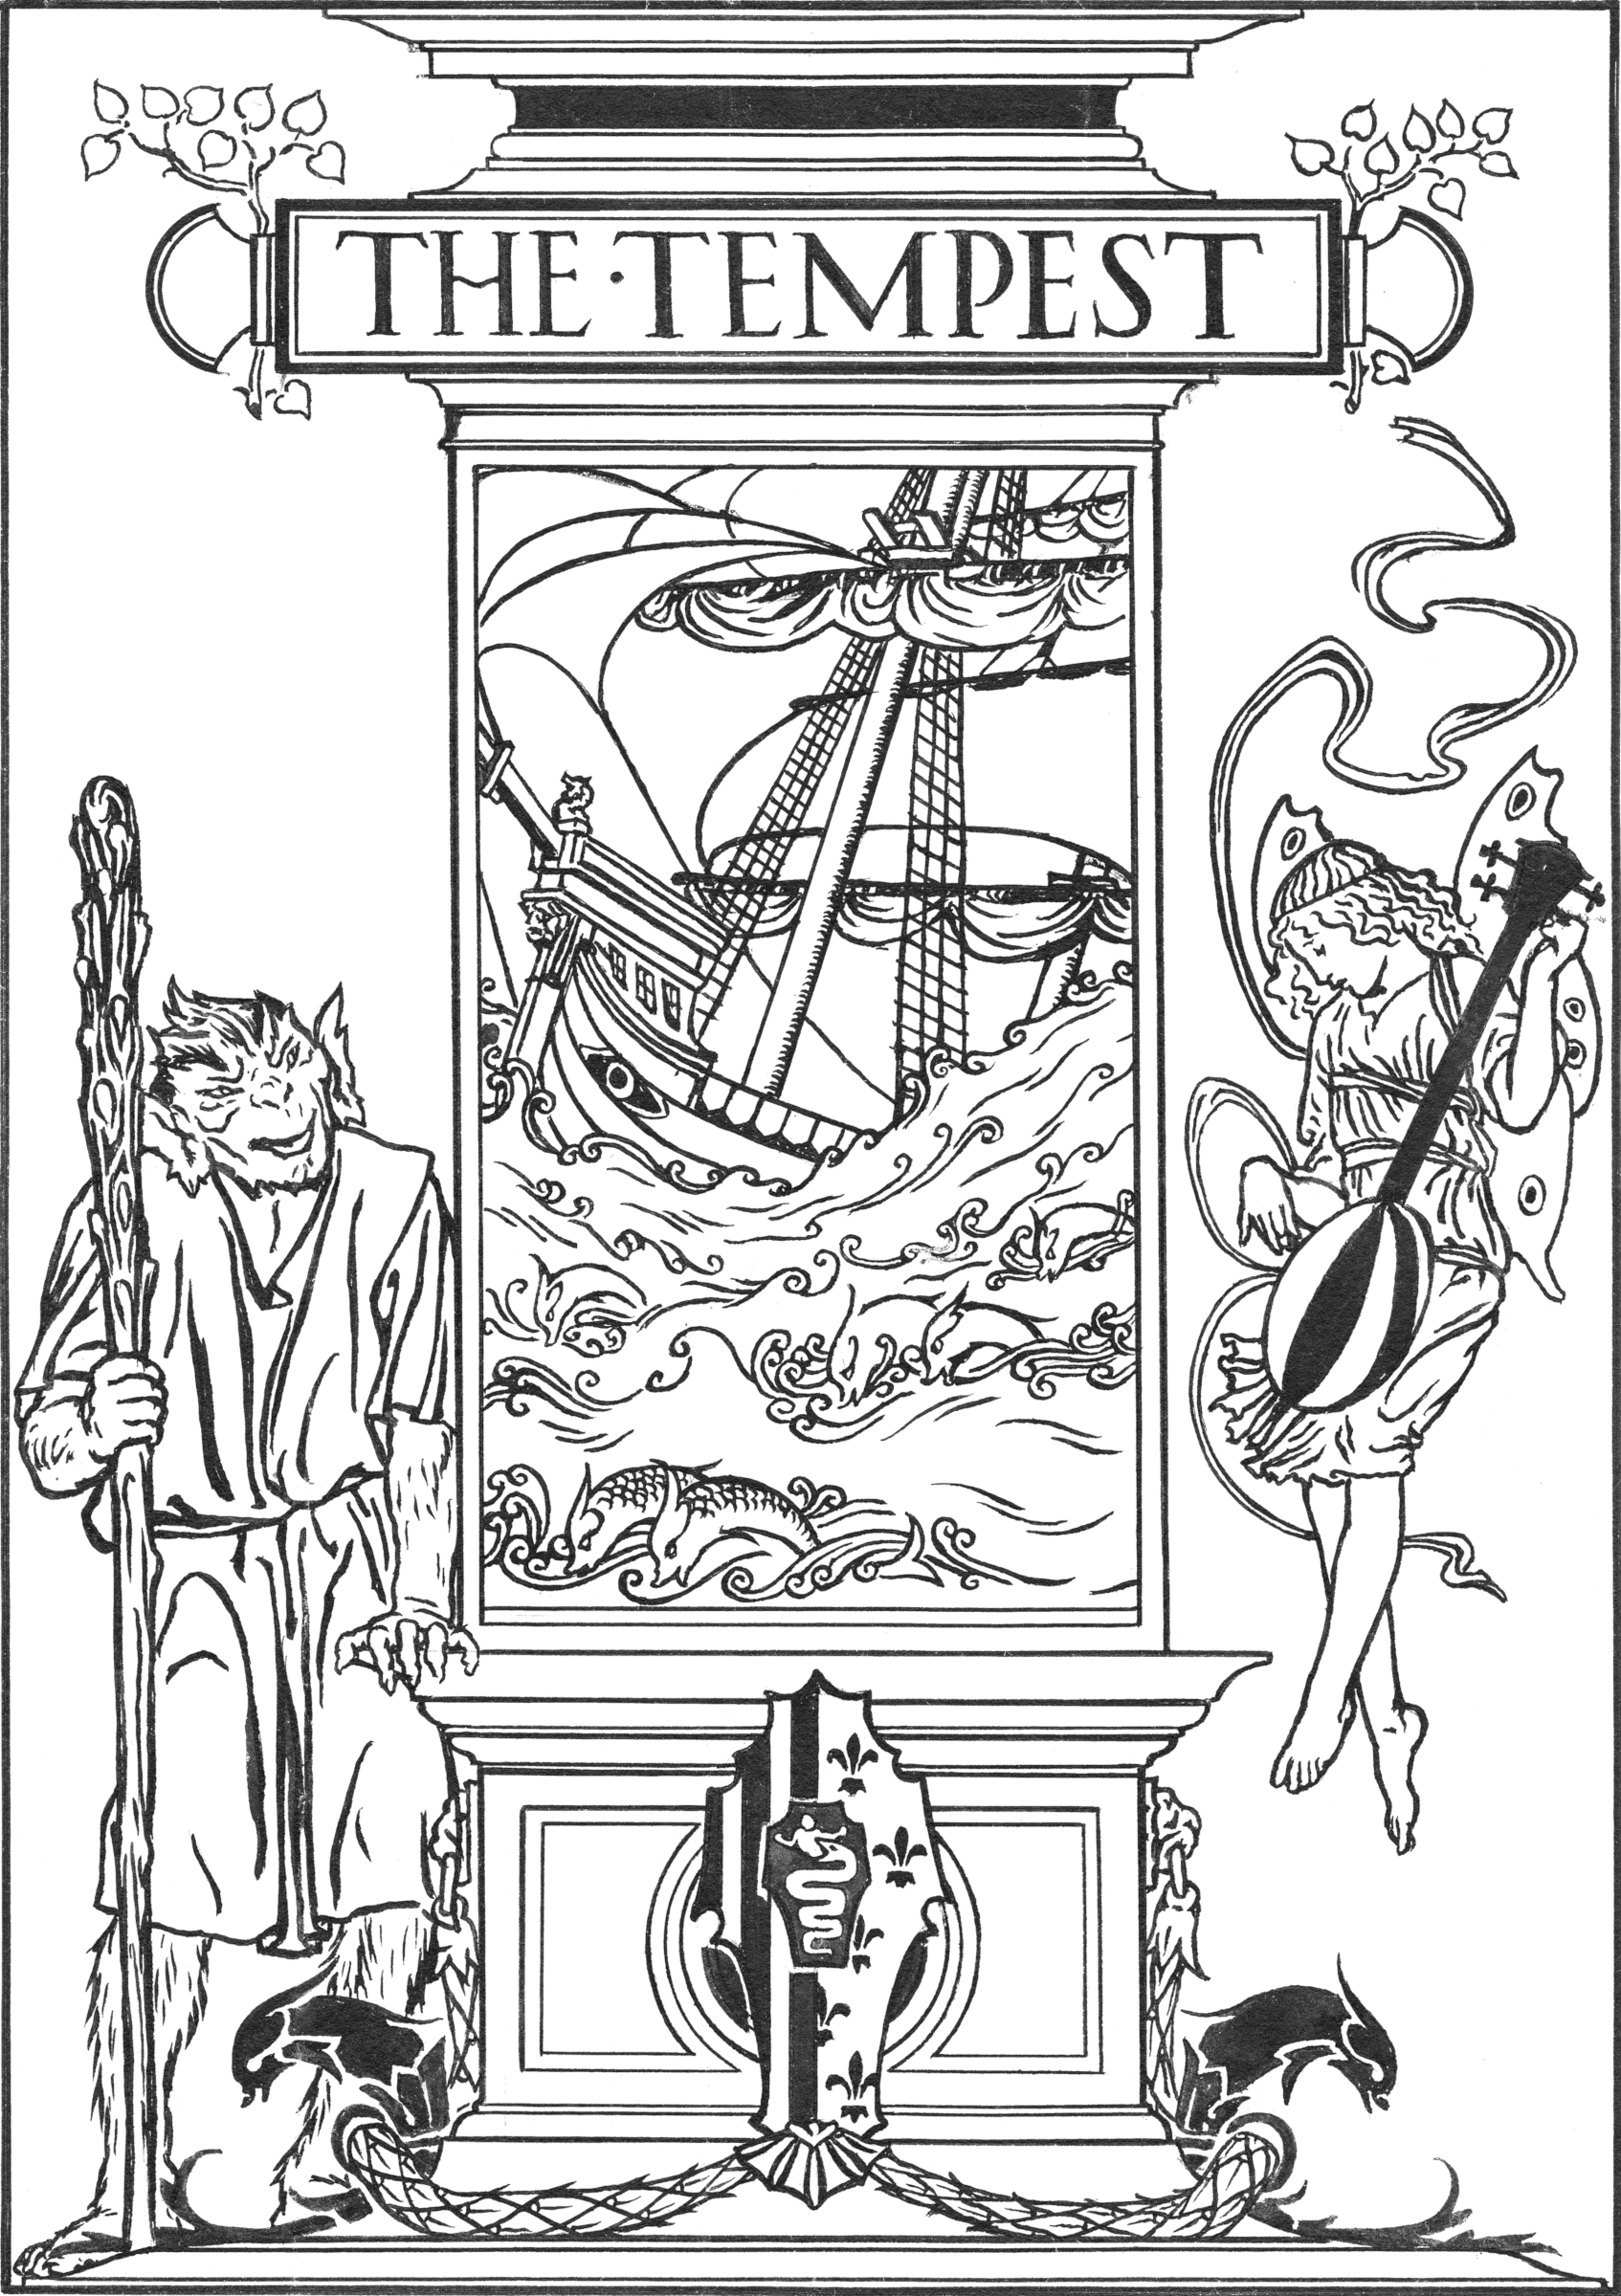
\includepdf[width=\textwidth]{images/cover.jpg}
		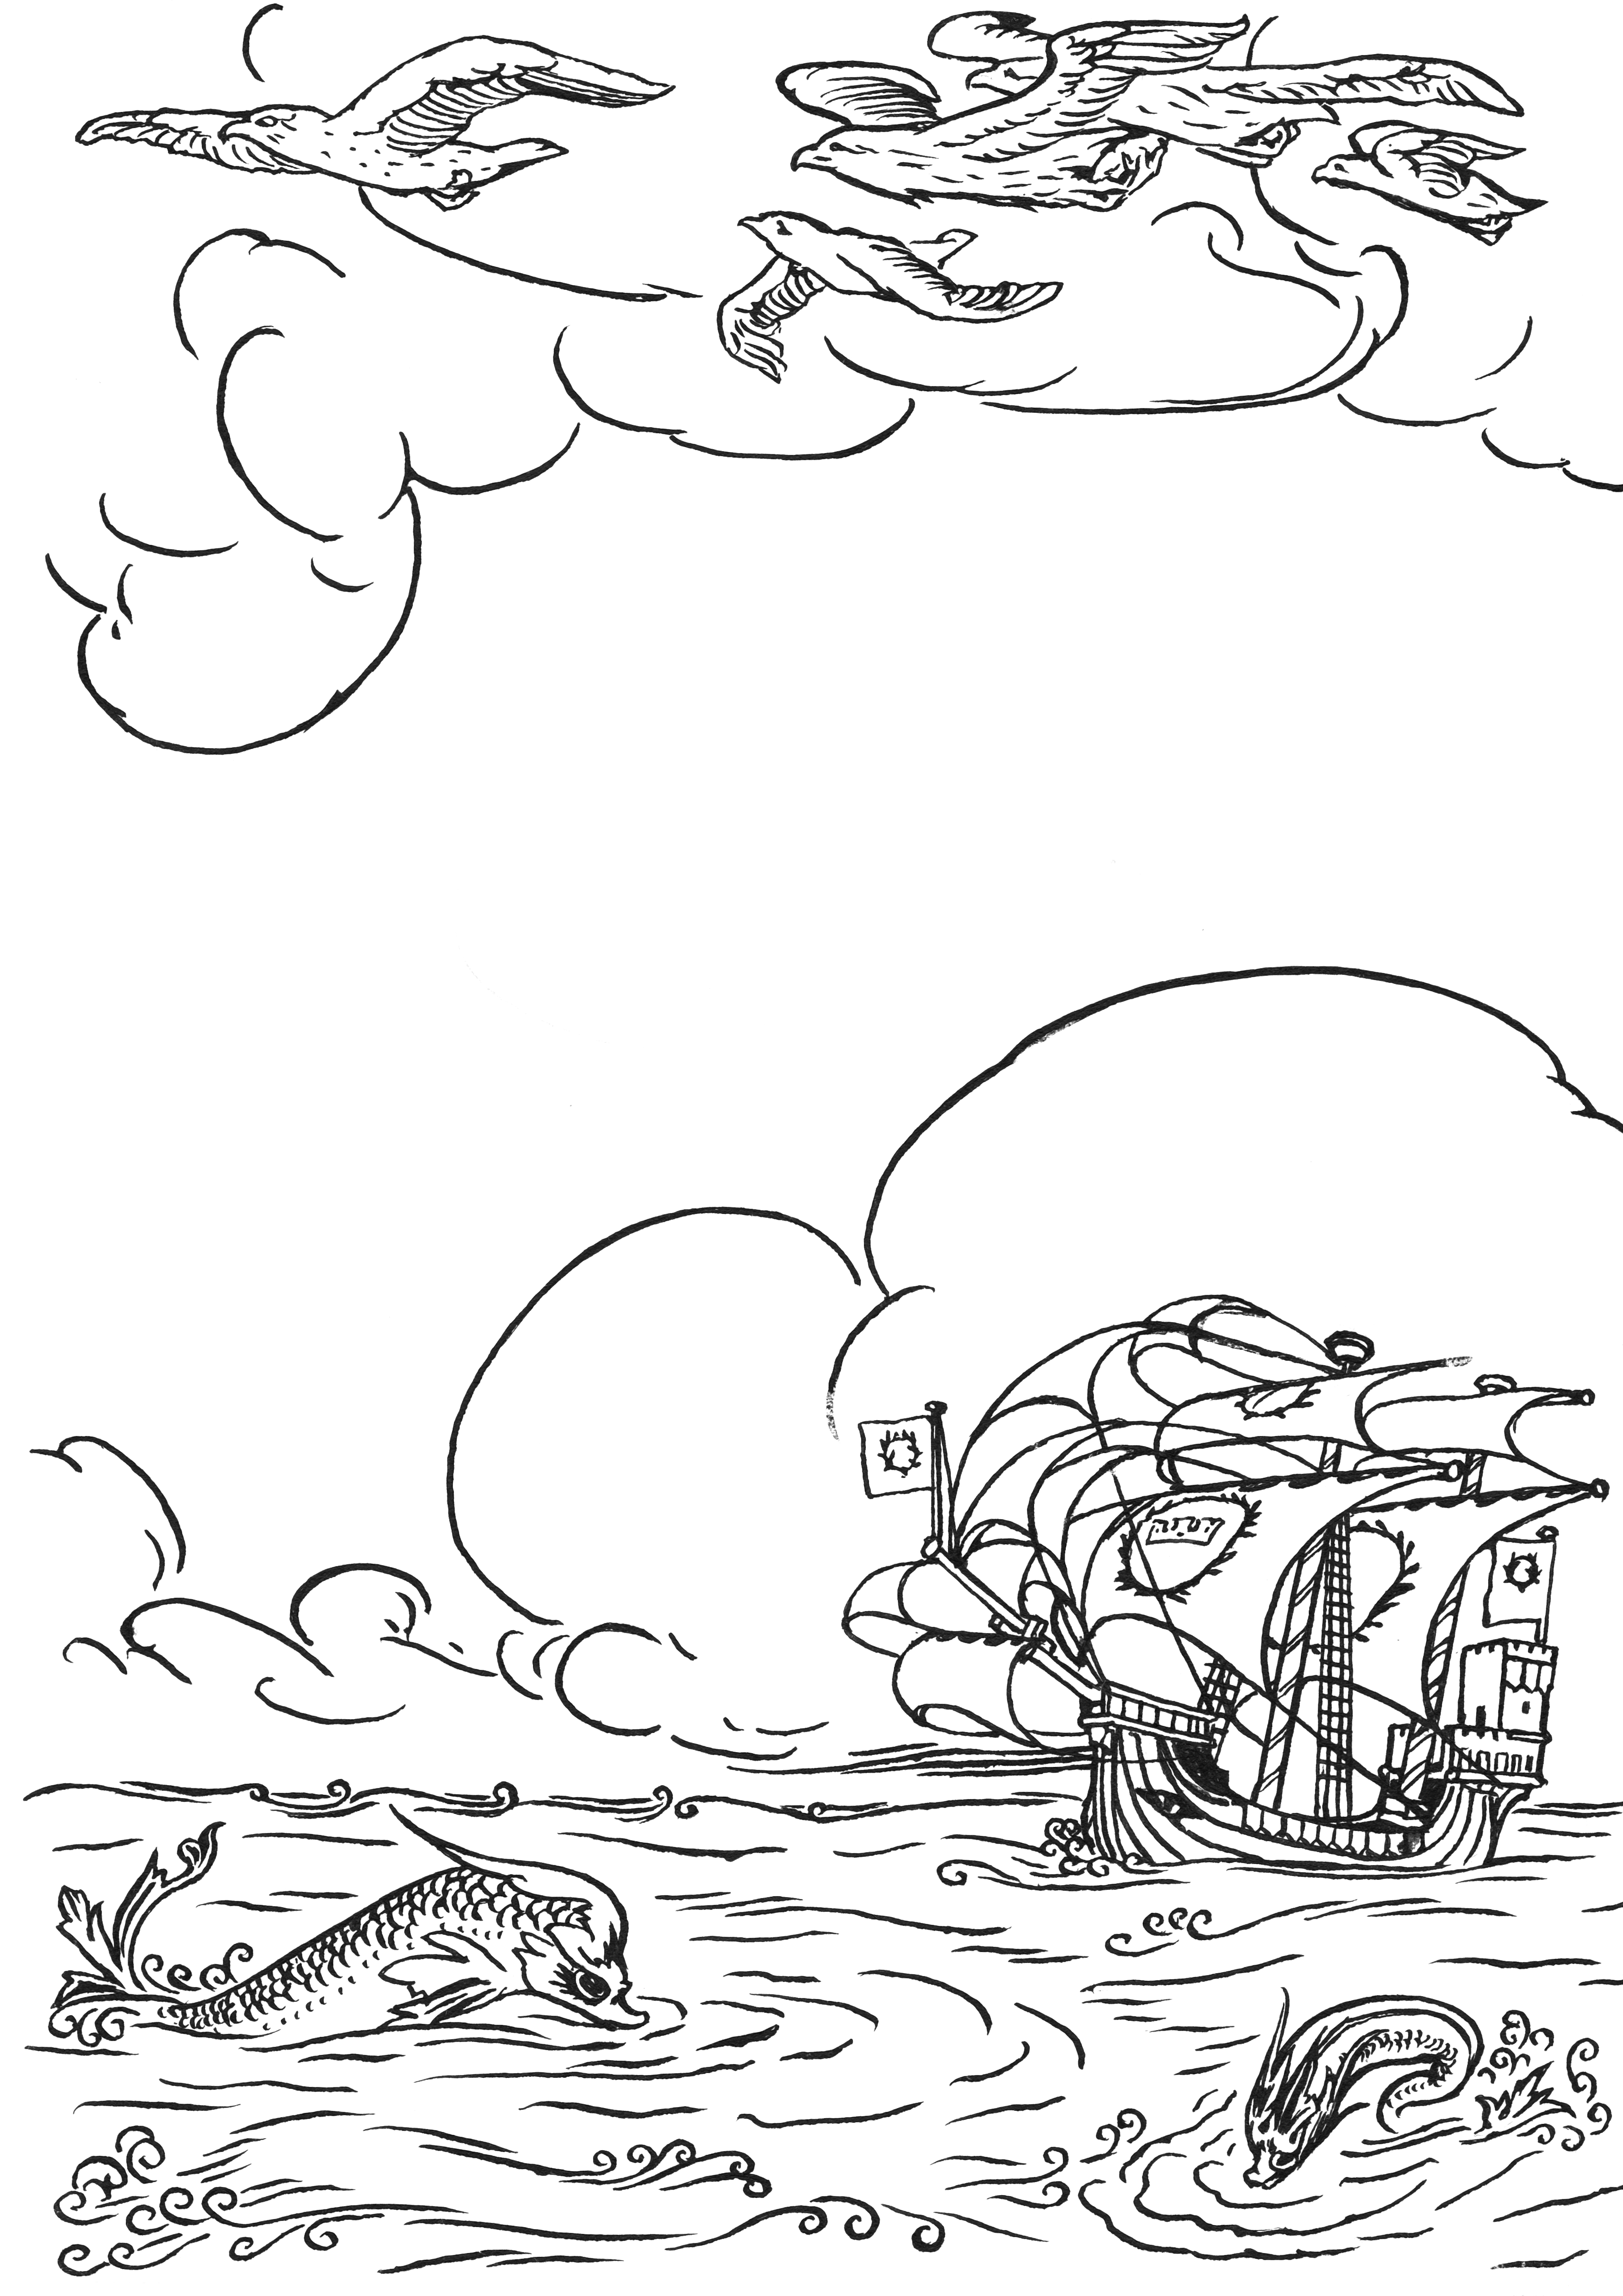
\includepdf[width=1.1\textwidth]{images/endpaper2.jpg}
		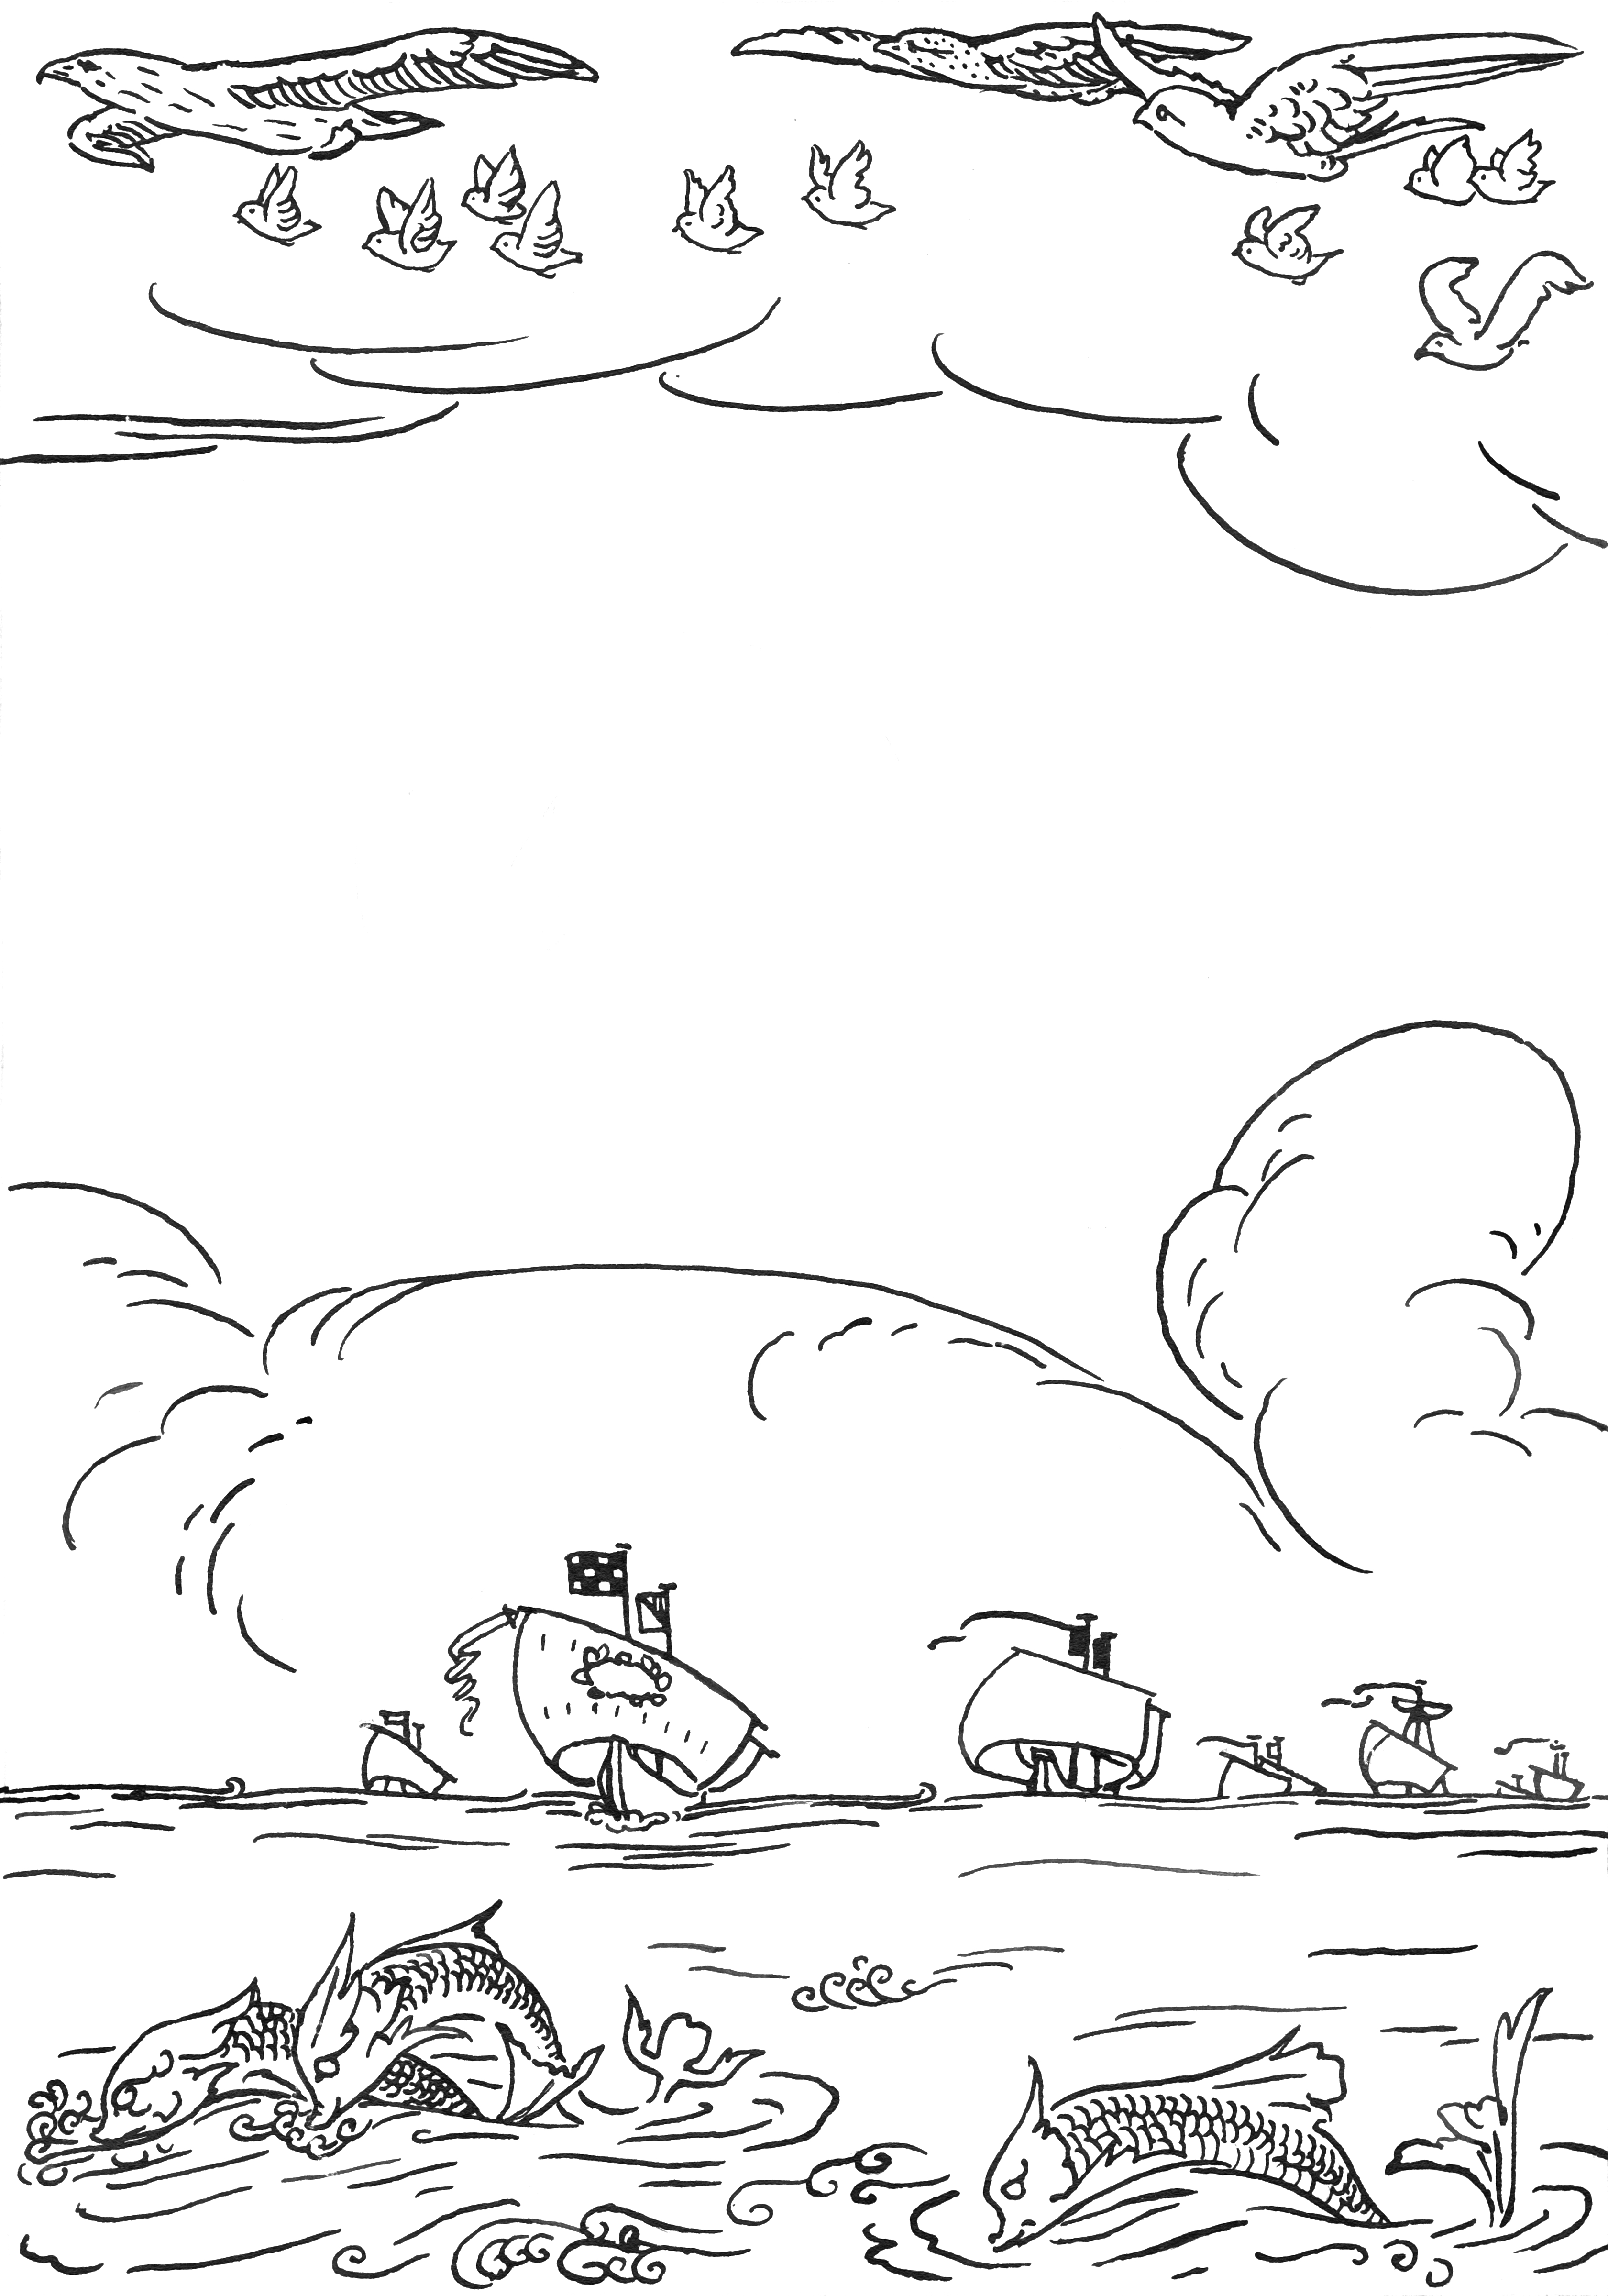
\includepdf[width=1.1\textwidth]{images/endpaper1.jpg}
		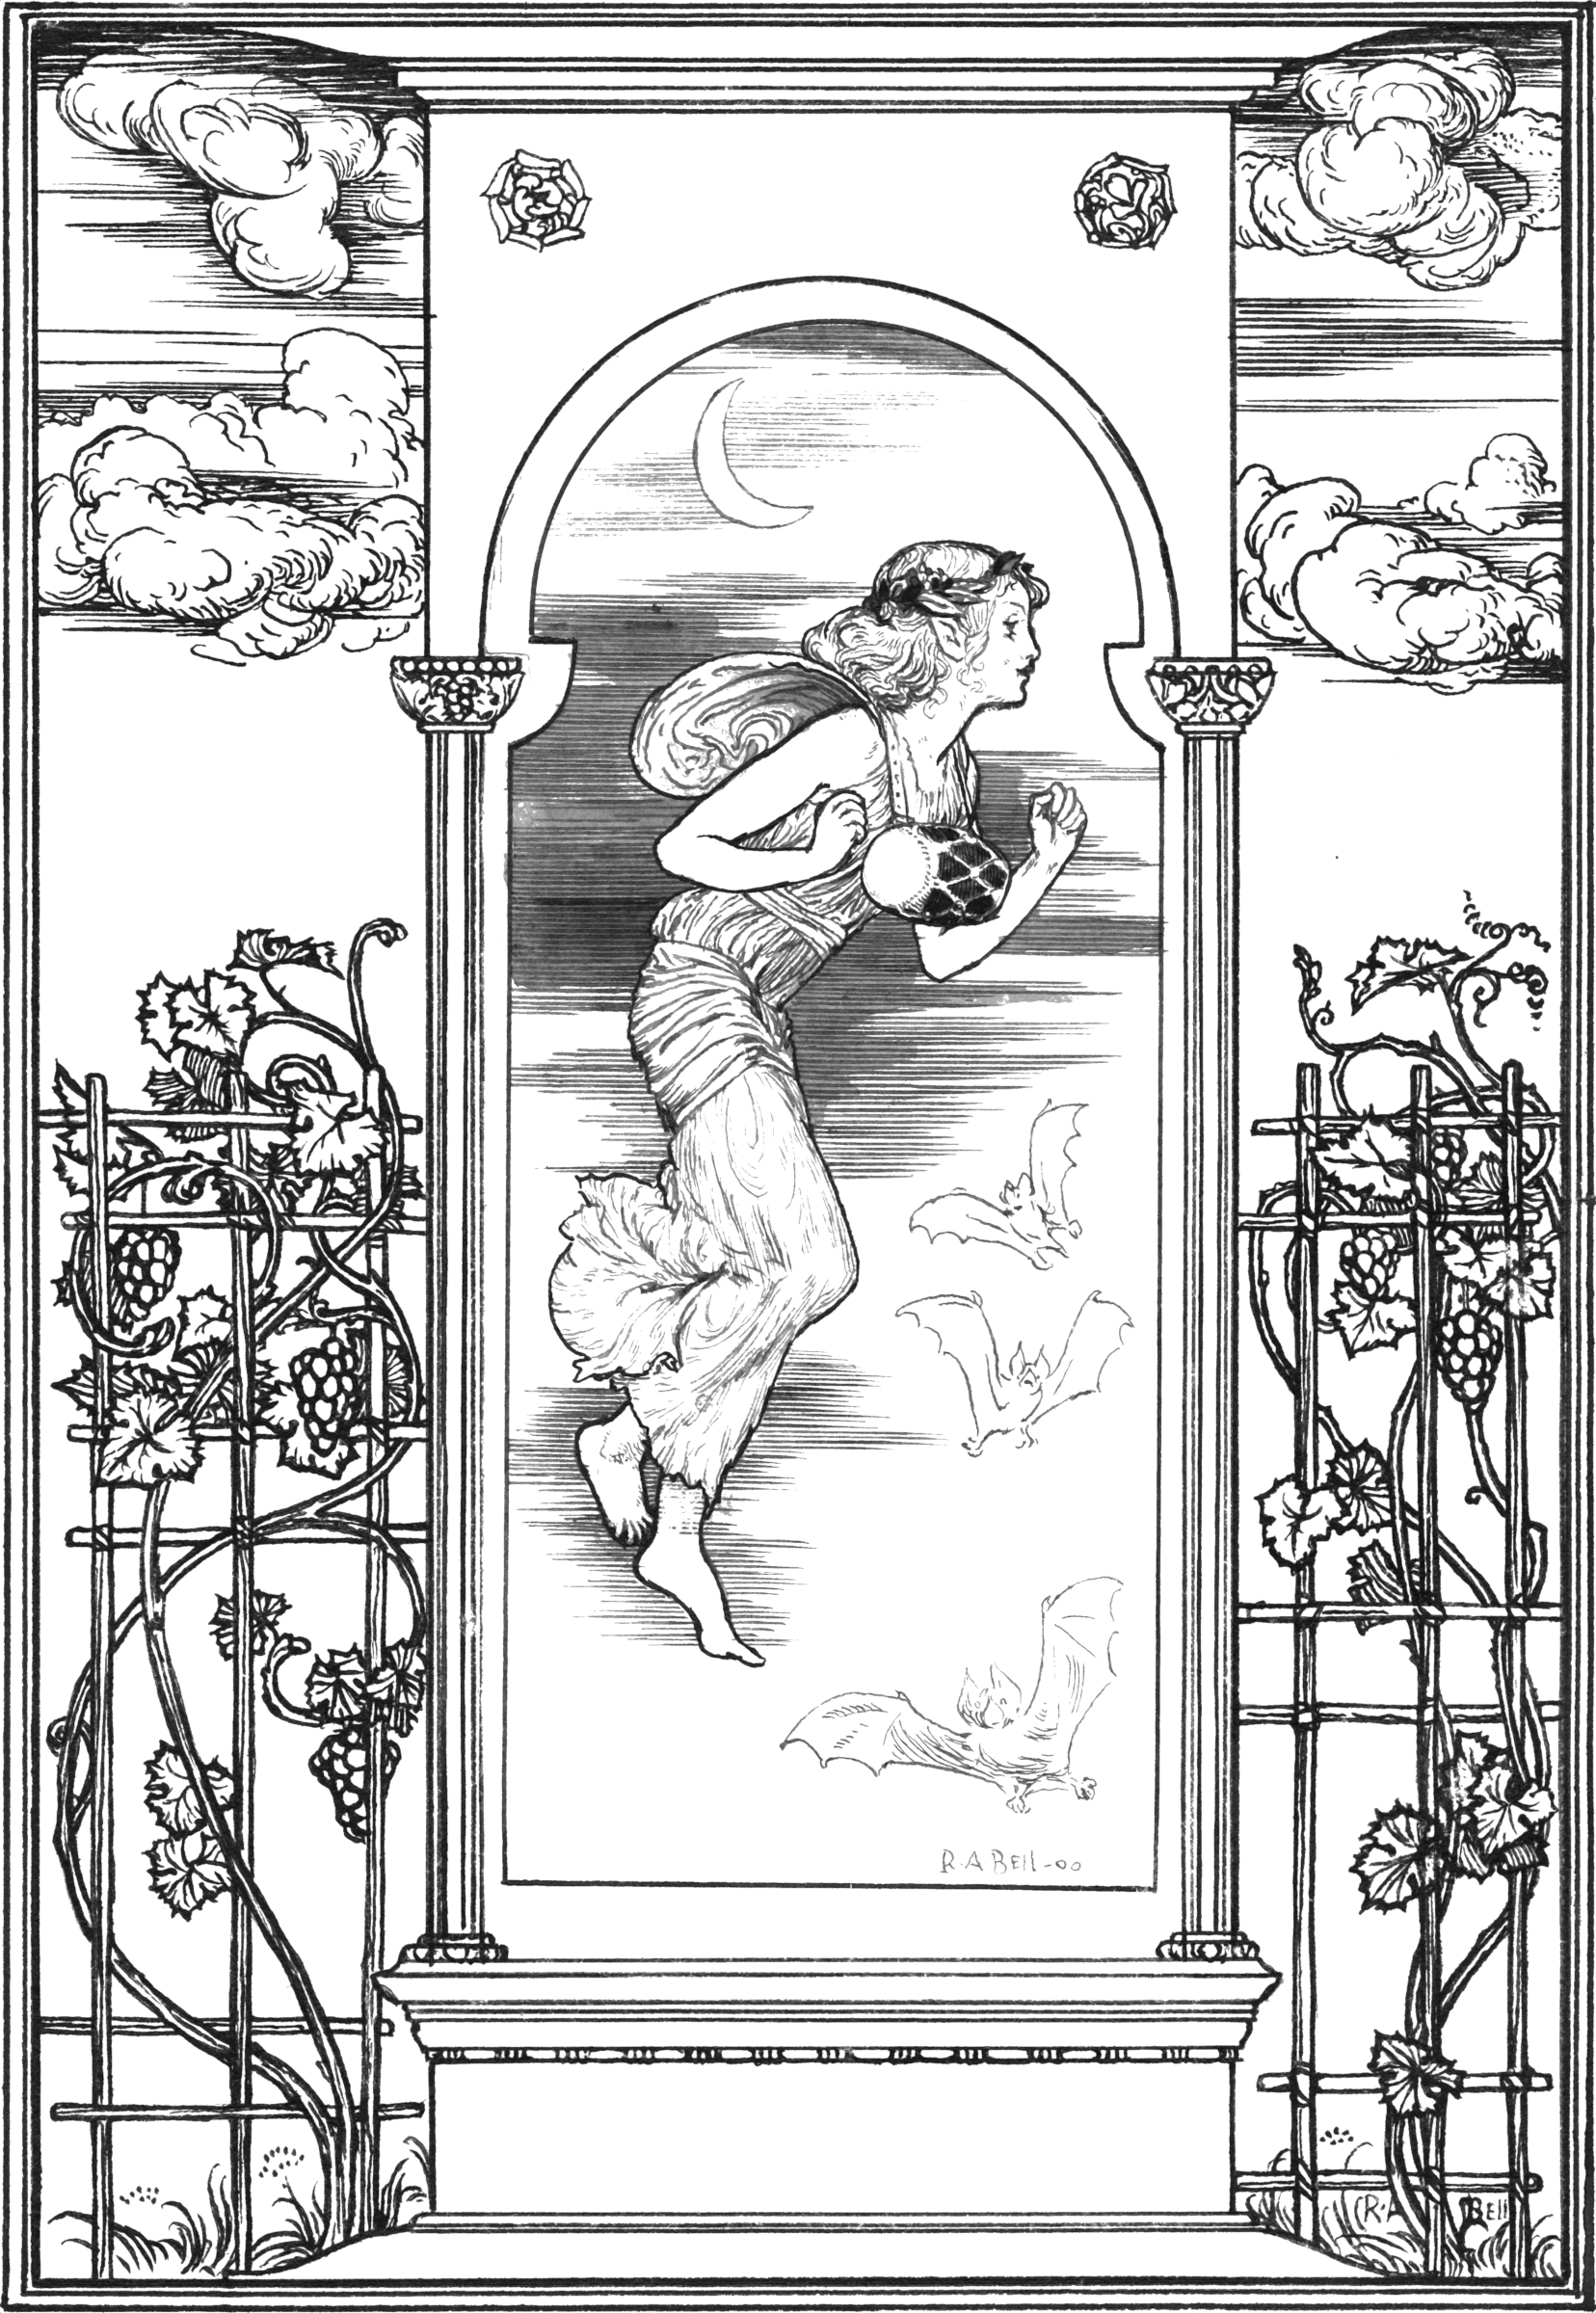
\includepdf[width=\textwidth]{images/arielbat.jpg}
		
\includepdf[width=\textwidth]{images/archpage.jpg}
		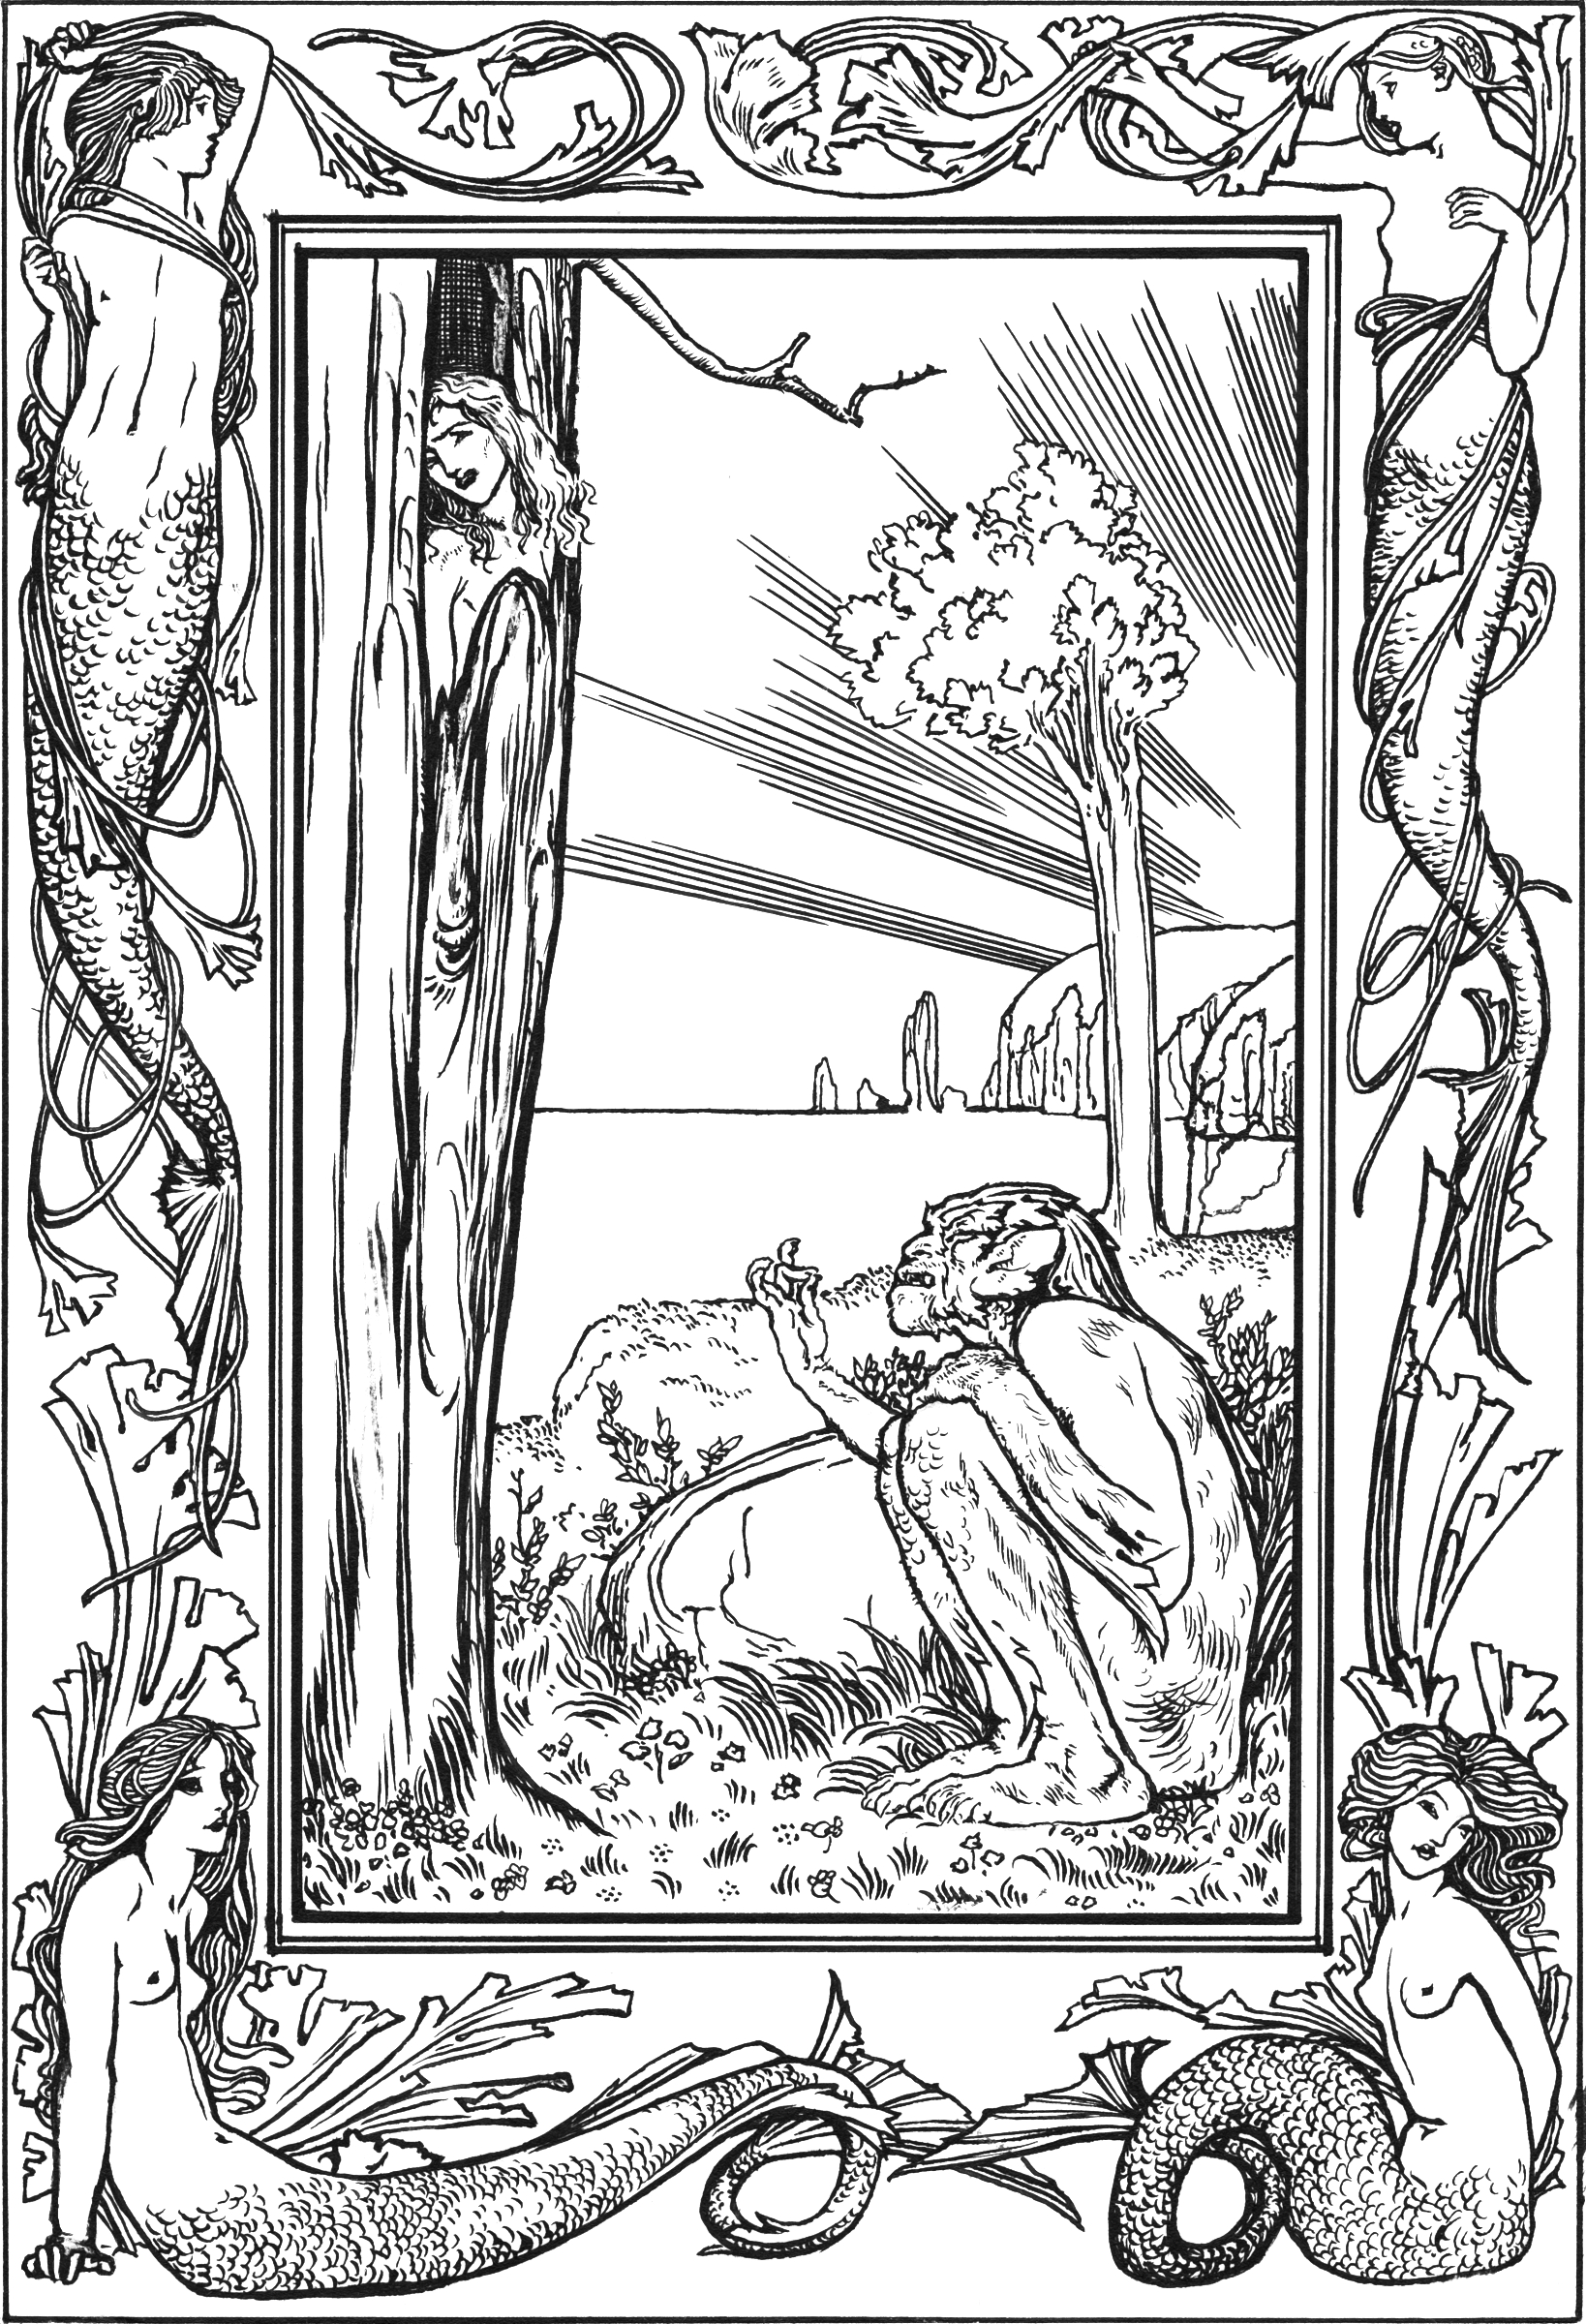
\includepdf[width=\textwidth]{images/clovenpine.jpg}
		\tableofcontents
		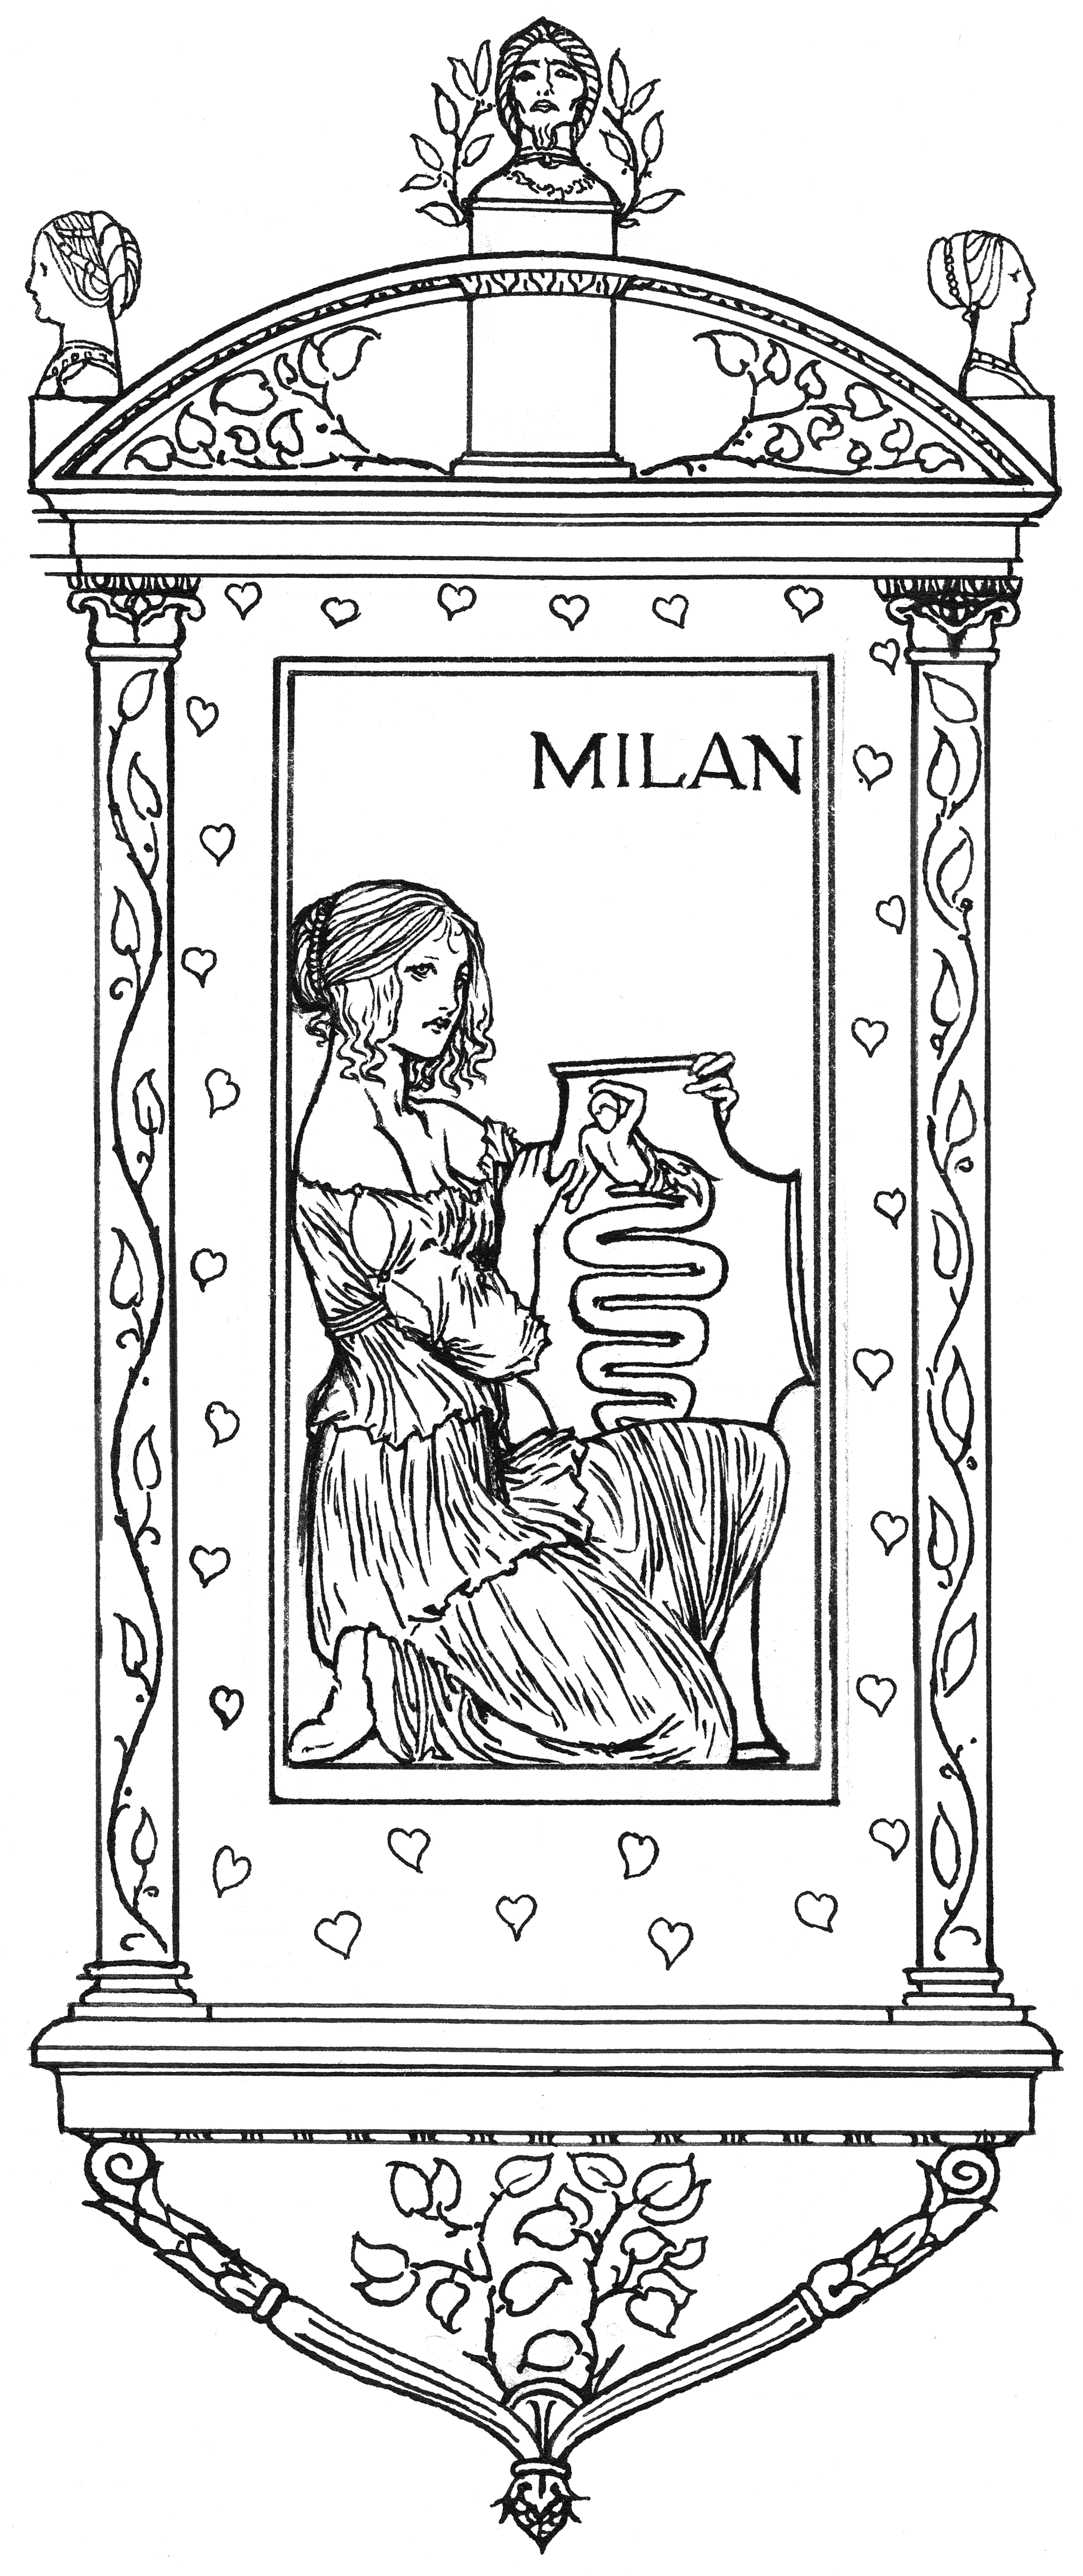
\includepdf[width=.65\textwidth]{images/milan.jpg}
		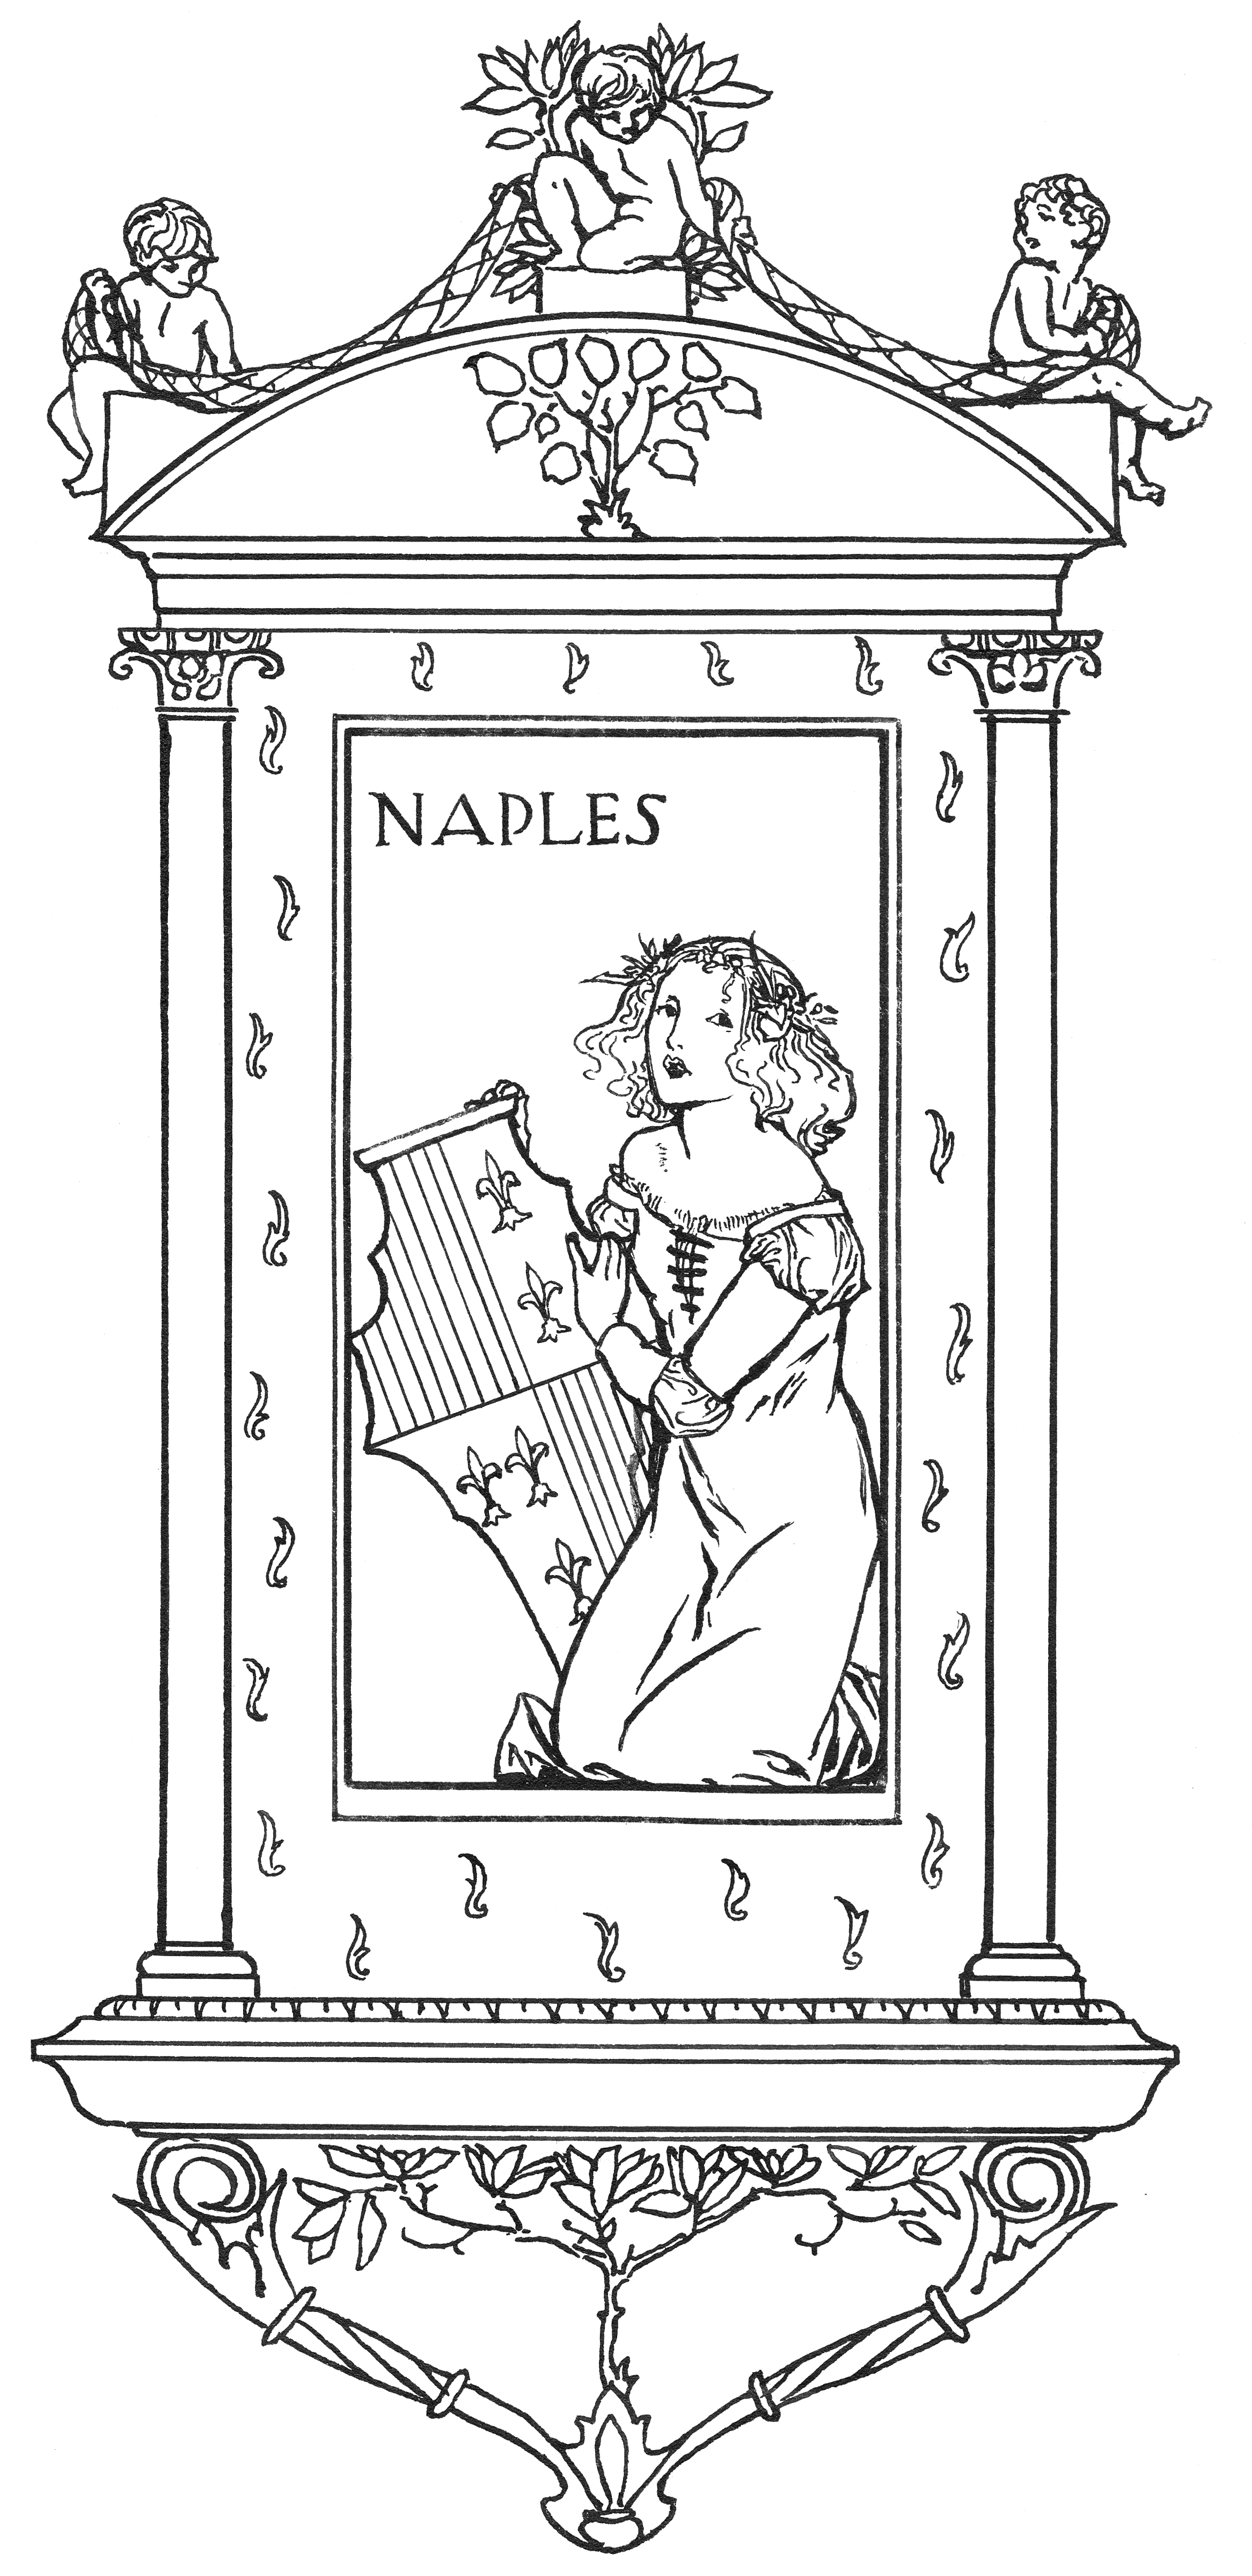
\includepdf[width=.75\textwidth]{images/naples.jpg}
		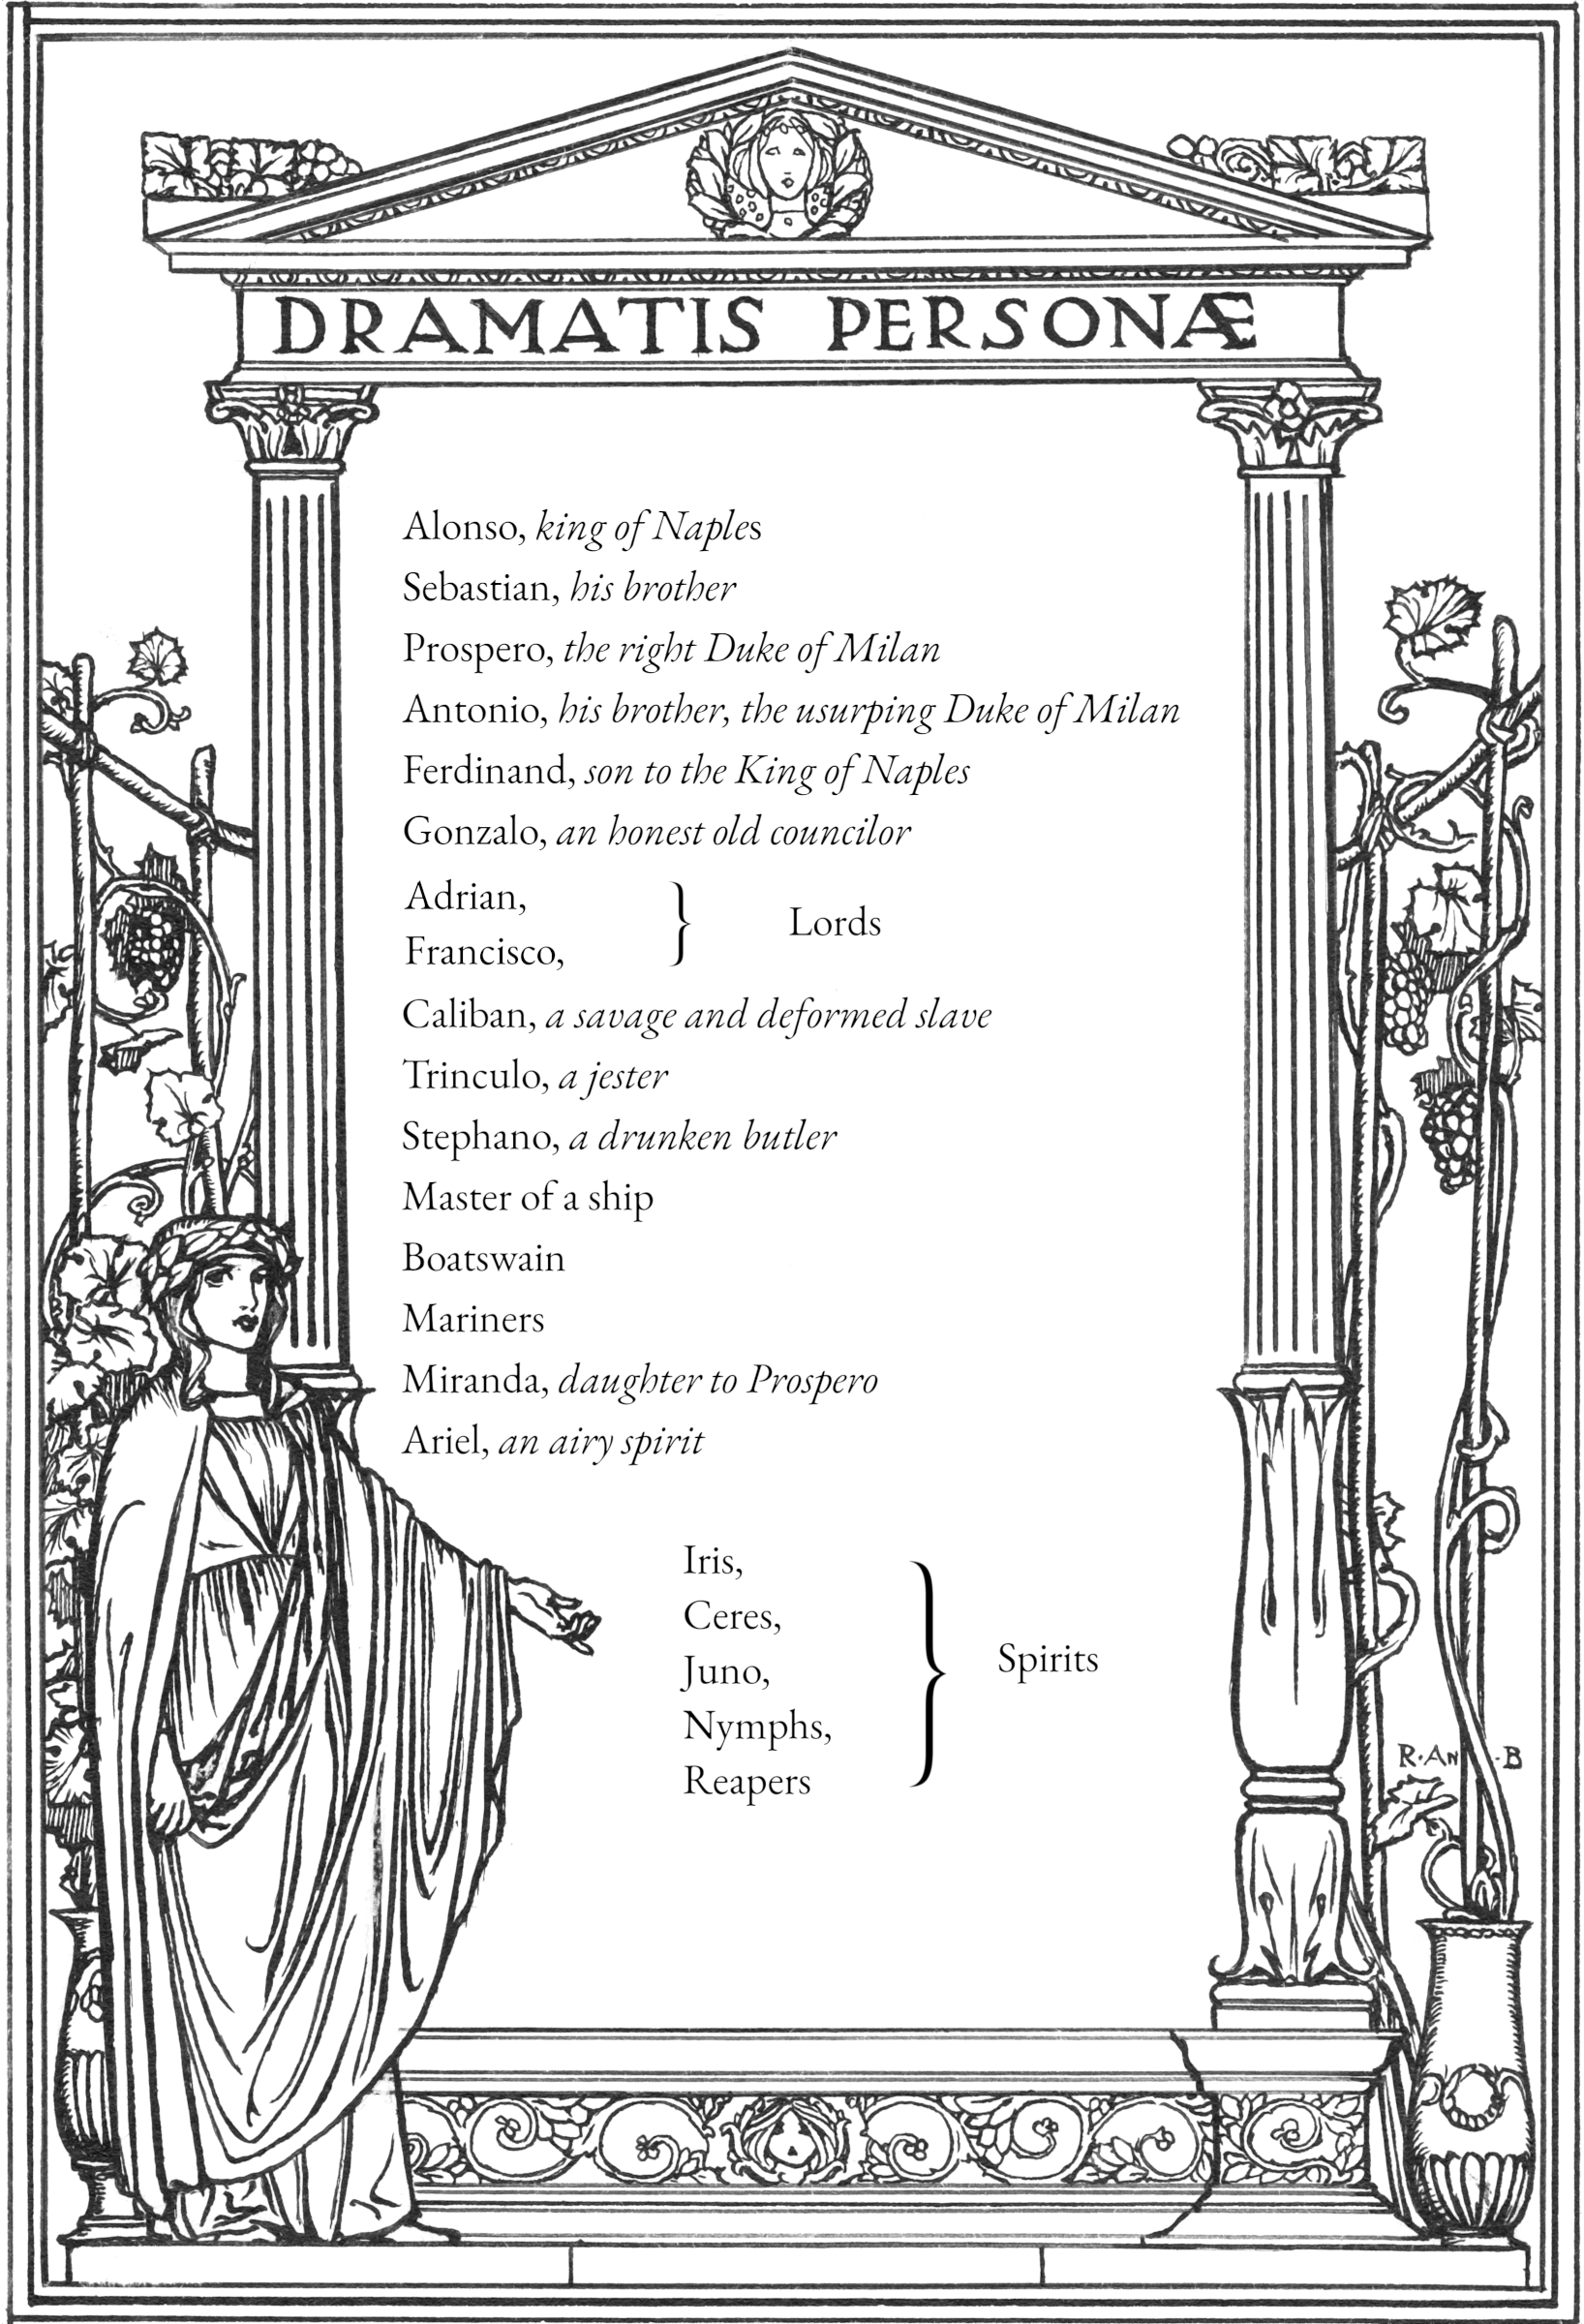
\includepdf[width=\textwidth]{images/dramper.jpg}
	\end{a4}
\end{pictures}

\begin{placeholder}
\cleardoubleoddpage
\end{placeholder}




\mainmatter
\KOMAoptions{headings=openright}

%!TeX root=../tempestrackham.tex

\Act*{1}
\Scene*{1}[On a ship at sea: a tempestuous noise of thunder and lightning heard.]

\begin{figure}[t]
	\centering
	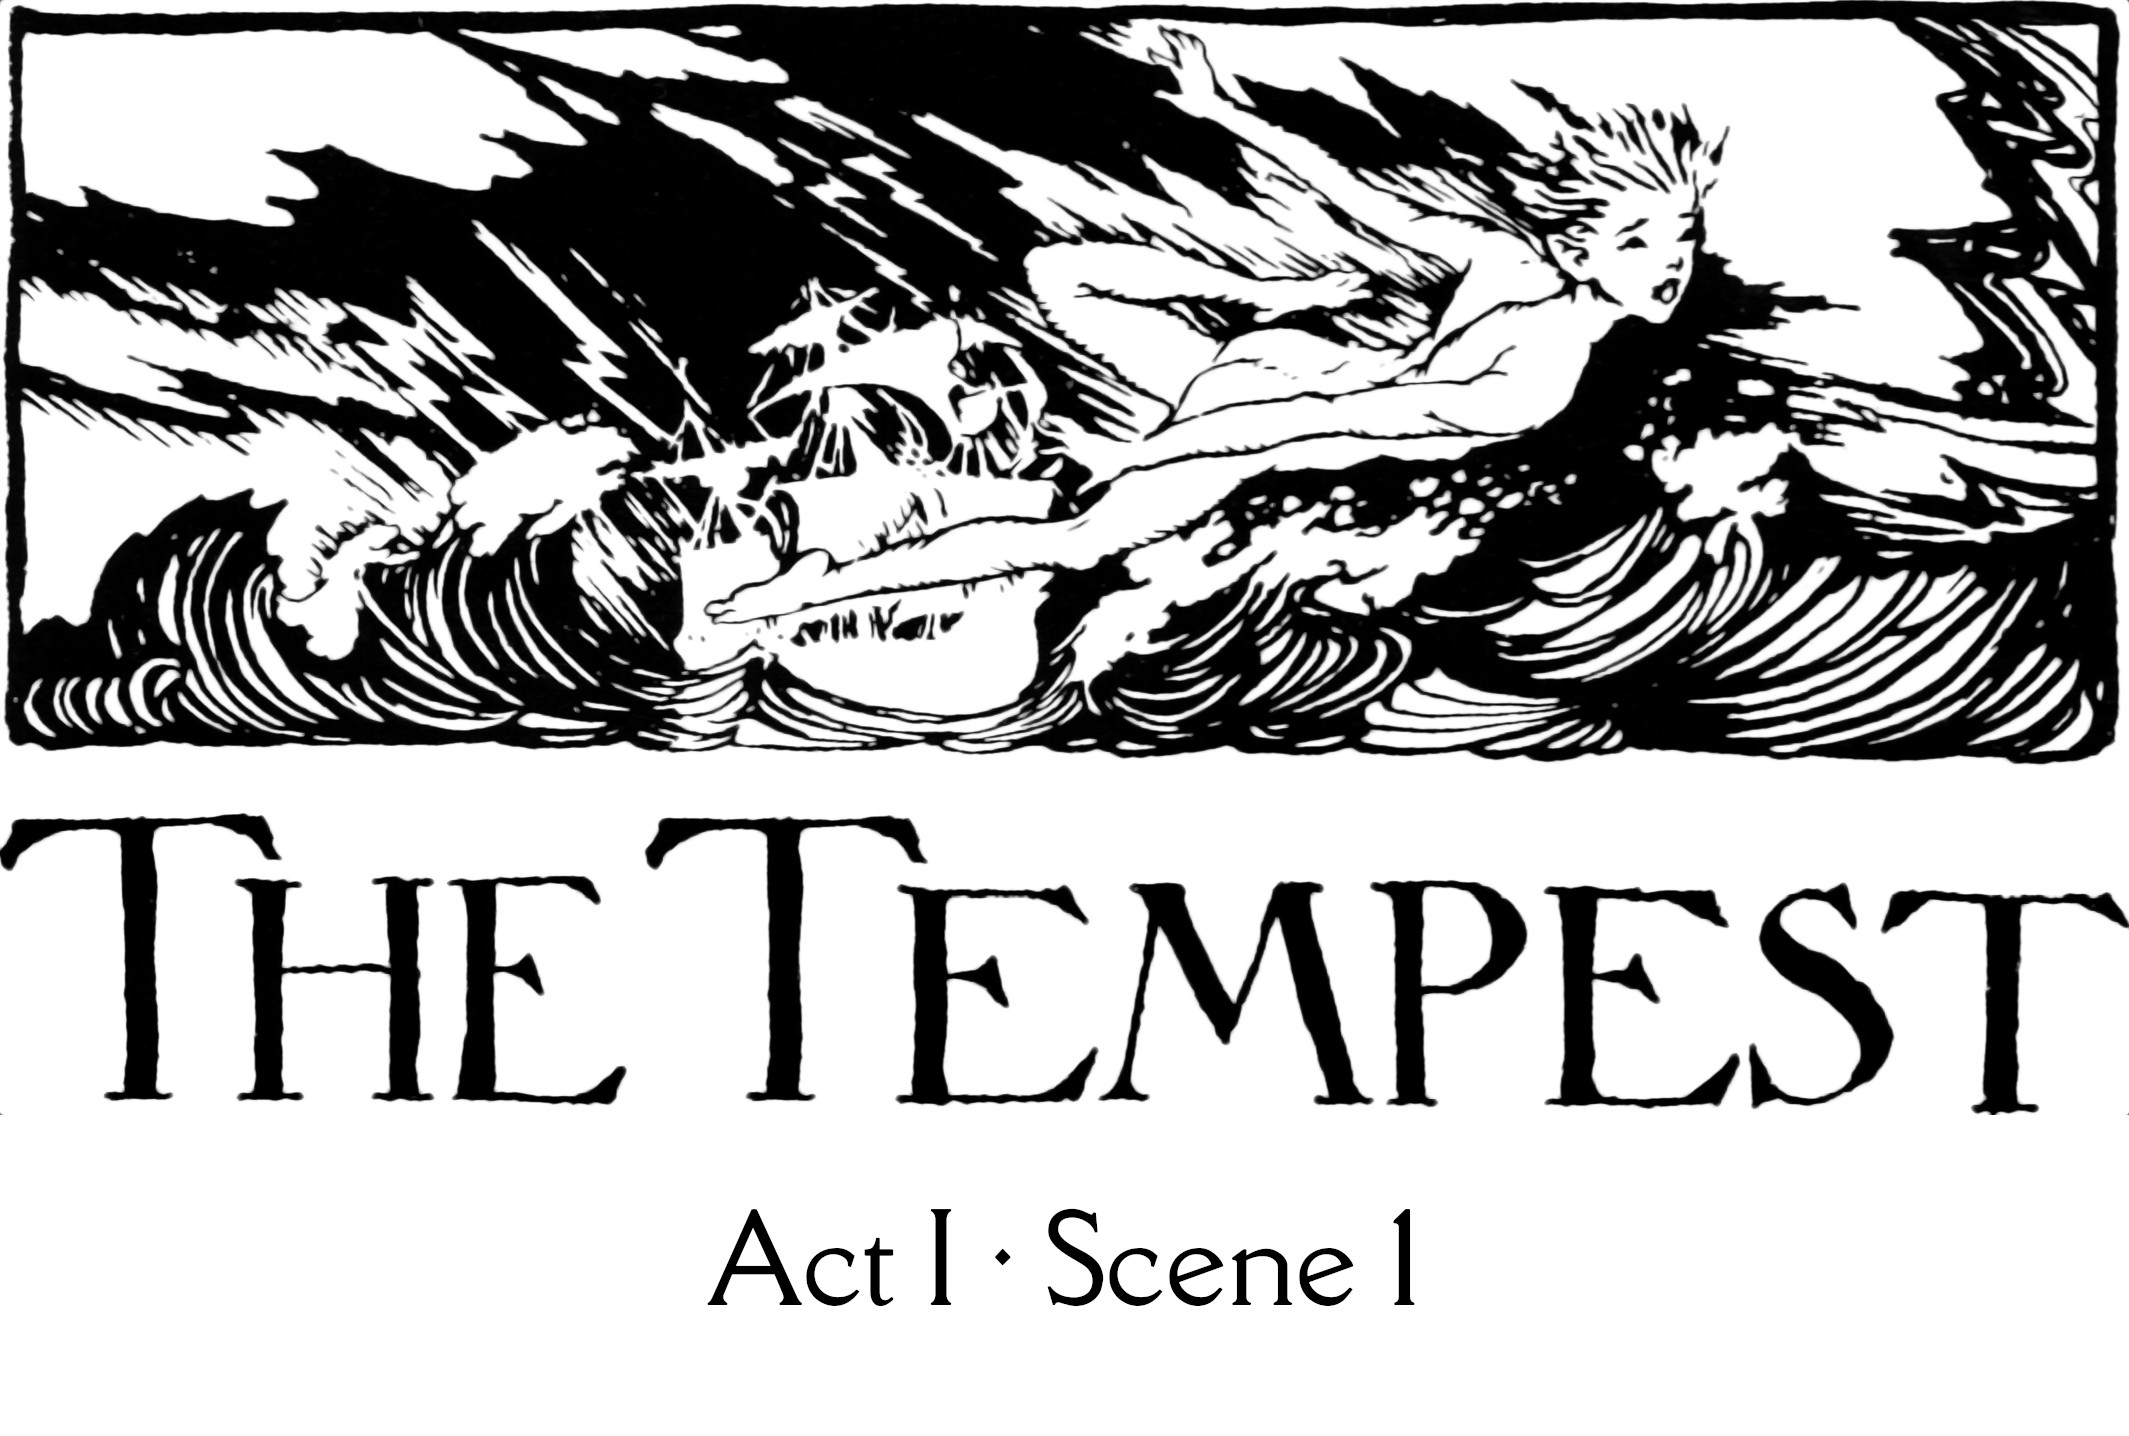
\includegraphics[width=\textwidth]{1ihead}
\end{figure}

\begin{letter}

\end{letter}

\vspace{\textsink}

\textit{(On a ship at sea: a tempestuous noise of thunder and lightning heard.)}\centering
\enter{a \textsc{Master} and a \textsc{Boatswain}}

\verseline[Master]{Boatswain!}
\verseline[Boatswain]{Here, master: what cheer?}
\verseline[Master]{Good, speak to the mariners: fall to't, yarely, or we run ourselves aground: bestir, bestir.}

\begin{prose_speech}[Boatswain] Heigh, my hearts! cheerly, cheerly, my hearts! yare, yare! Take in the topsail. Tend to the master's whistle. Blow, till thou burst thy wind, if room enough!
\end{prose_speech}

\enter{\textsc{Alonso}, \textsc{Sebastian}, \textsc{Antonio}, \textsc{Ferdinand}, \textsc{Gonzalo}, and others}

\begin{prose_speech}[Alonso] Good boatswain, have care. Where's the master? Play the men.
\end{prose_speech}


\begin{prose_speech}[Boatswain] I pray now, keep below.\end{prose_speech}

\begin{prose_speech}[Antonio] Where is the master, boatswain?\end{prose_speech}

\begin{prose_speech}[Boatswain] Do you not hear him? You mar our labour: keep your cabins: you do assist the storm.
\end{prose_speech}

\begin{prose_speech}[Gonzalo] Nay, good, be patient.\end{prose_speech}

\begin{prose_speech}[Boatswain] When the sea is. Hence! What cares these roarers for the name of king? To cabin: silence! trouble us not.\end{prose_speech}

\begin{prose_speech}[Gonzalo] Good, yet remember whom thou hast aboard.\end{prose_speech}

\begin{letter}
	\enlargethispage{\baselineskip}
\end{letter}
\begin{prose_speech}[Boatswain] None that I more love than myself. You are a counsellor; if you can command these elements to silence, and work the peace of the present, we will not hand a rope more; use your authority: if you cannot, give thanks you have lived so long, and make yourself ready in your cabin for the mischance of the hour, if it so hap. Cheerly, good hearts! Out of our way, I say.
\end{prose_speech}

\exit{\textsc{Boatswain}}

\begin{prose_speech}[Gonzalo] I have great comfort from this fellow: methinks he hath no drowning mark upon him; his complexion is perfect gallows. Stand fast, good Fate, to his hanging: make the rope of his destiny our cable, for our own doth little advantage. If he be not born to be hanged, our case is miserable.
\end{prose_speech}

\exit{\textsc{Gonzalo}, with \textsc{Alonso}, \textsc{Sebastian}, and the other courtiers.}


\enter{\textsc{Boatswain}}

\begin{prose_speech}[Boatswain] Down with the topmast! yare! lower, lower! Bring her to try with main-course.
\stage{A cry within}
A plague upon this howling! they are louder than the weather or our office.
\stage{Re-enter \textsc{Sebastian}, \textsc{Antonio}, and \textsc{Gonzalo}}
Yet again! what do you here? Shall we give o'er and drown? Have you a mind to sink?
\end{prose_speech}

\begin{prose_speech}[Sebastian] A pox o' your throat, you bawling, blasphemous, incharitable dog!
\end{prose_speech}

\begin{prose_speech}[Boatswain] Work you then.
	\end{prose_speech}

\begin{prose_speech}[Antonio] Hang, cur! hang, you whoreson, insolent noisemaker! We are less afraid to be drowned than thou art.
\end{prose_speech}

\begin{prose_speech}[Gonzalo] I'll warrant him for drowning; though the ship were no stronger than a nutshell and as leaky as an unstanched wench.
\end{prose_speech}

\begin{prose_speech}[Boatswain] Lay her a-hold, a-hold! set her two courses off to sea again; lay her off.
\end{prose_speech}

\enter{\textsc{Mariners} wet}

\begin{prose_speech}[Mariners] All lost! to prayers, to prayers! all lost!
	\end{prose_speech}

\exit{\textsc{Mariners}}

\begin{prose_speech}[Boatswain] What, must our mouths be cold?
	\end{prose_speech}

\begin{verse_speech}[Gonzalo] The king and prince at prayers! let's assist them,\\ For our case is as theirs.
\end{verse_speech}

\begin{verse_speech}[Sebastian] \hspace{\widthof{For our case is as theirs.}}I'm out of patience.\end{verse_speech}

\begin{verse_speech}[Antonio] We are merely cheated of our lives by drunkards:\\
This wide-chapp'd rascal—would thou mightst lie drowning\\
The washing of ten tides!\end{verse_speech}

\exit{\textsc{Boatswain}}

\begin{verse_speech}[Gonzalo] \hspace{\widthof{The washing of ten tides!}}He'll be hang'd yet,\\
Though every drop of water swear against it\\
And gape at widest to glut him.
\end{verse_speech}

\stage{A confused noise within: <Mercy on us!>—<We split, we split!>—<Farewell, my wife and children!>—<Farewell, brother!>—<We split, we split, we split!>}


\begin{verse_speech}[Antonio] Let's all sink with the king.\end{verse_speech}

\begin{verse_speech}[Sebastian] Let's take leave of him.\end{verse_speech}

\exit{\textsc{Antonio} and \textsc{Sebastian}}

\begin{prose_speech}[Gonzalo] Now would I give a thousand furlongs of sea for an acre of barren ground, long heath, brown furze, any  thing. The wills above be done! but I would fain die a dry death.
\end{prose_speech}

\exeunt{}

\begin{figure}[b]
	\centering
	
\includegraphics[width=\textwidth]{fish}
\end{figure}



\Scene{2}[The island. Before \textsc{Prospero's} cell.]


	\begin{figure}[t]
		\centering
		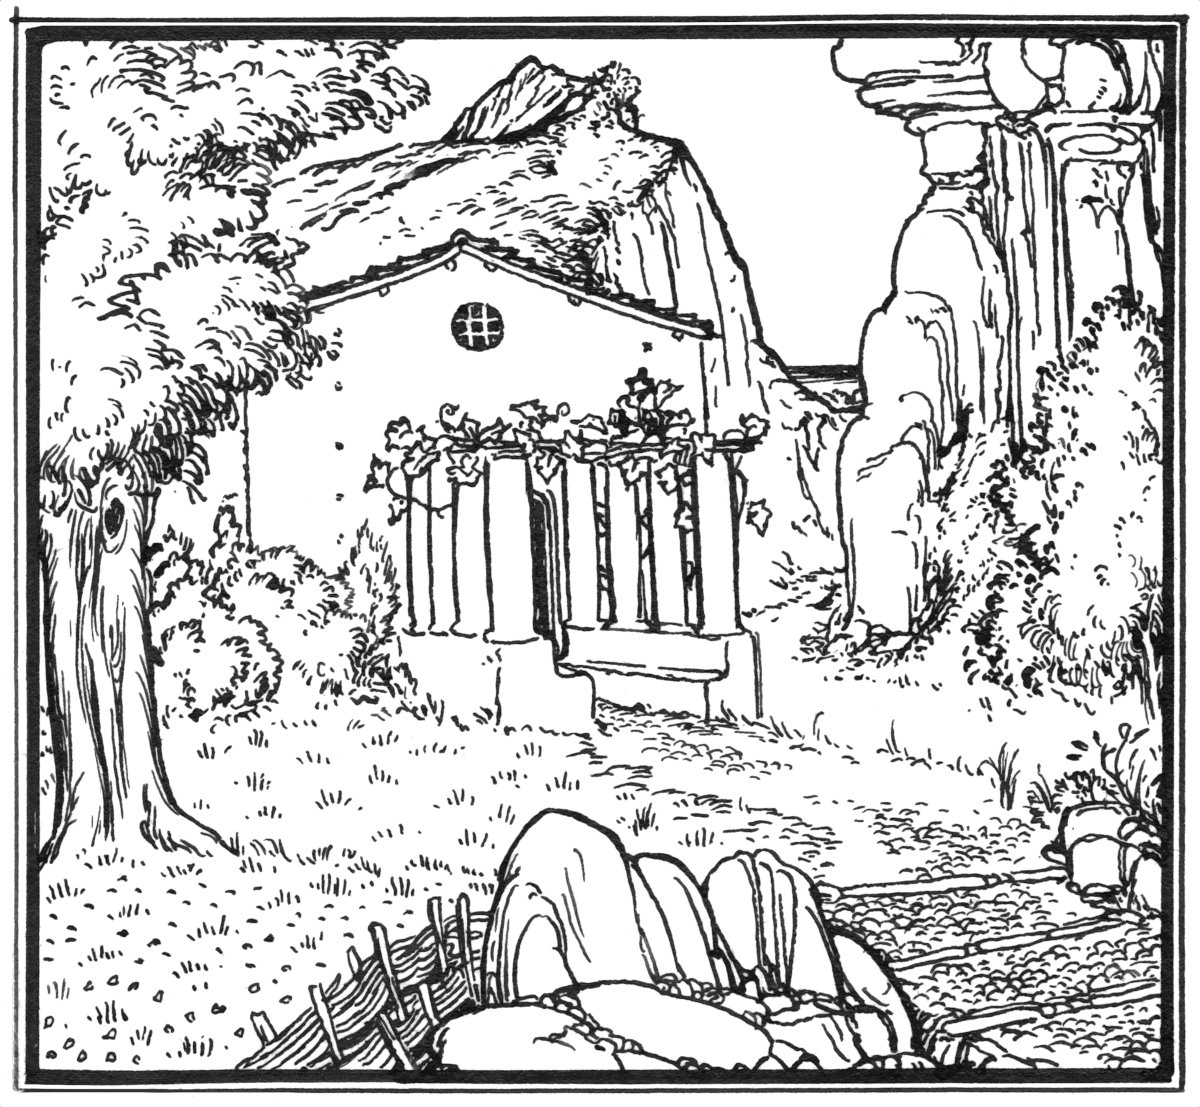
\includegraphics[width=\headerwidth]{1iiheadpiece}
	\end{figure}

	\enter{\textsc{Prospero} and \textsc{Miranda}}
	
\begin{letter}
	\begin{tikzpicture}[remember picture, overlay]
		\node (dropcap) at ($(current page.west)+(2.25cm,-6.5cm)$) {
\includegraphics[width=0.125\linewidth]{1iidropcapI}};
	\end{tikzpicture}

	\begin{verse_speech}[Miranda] 
	\hspace{0.5em}f by your art, my dearest father, you have\\
	\hspace{1em}Put the wild waters in this roar, allay them.\\
	\hspace{1em}The sky, it seems, would pour down stinking pitch,\\
	But that the sea, mounting to the welkin's cheek,\\
	Dashes the fire out. O, I have suffered\\
	With those that I saw suffer: a brave vessel,\\
	Who had, no doubt, some noble creature in her,\\
	Dash'd all to pieces. O, the cry did knock\\
	Against my very heart. Poor souls, they perish'd.\\
	Had I been any god of power, I would\\
	Have sunk the sea within the earth or ere\\
	It should the good ship so have swallow'd and\\
	The fraughting souls within her.\\
	\end{verse_speech}
\end{letter}

\begin{a4}
	\begin{tikzpicture}[remember picture, overlay]
		\node (dropcap) at ($(current page.west)+(2.45cm,-5.4cm)$) {
\includegraphics[width=0.115\linewidth]{1iidropcapI}};
	\end{tikzpicture}

	\begin{verse_speech}[Miranda] 
	\hspace{1em}f by your art, my dearest father, you have\\
	\hspace{1em}Put the wild waters in this roar, allay them.\\
	\hspace{1em}The sky, it seems, would pour down stinking pitch,\\
	But that the sea, mounting to the welkin's cheek,\\
	Dashes the fire out. O, I have suffered\\
	With those that I saw suffer: a brave vessel,\\
	Who had, no doubt, some noble creature in her,\\
	Dash'd all to pieces. O, the cry did knock\\
	Against my very heart. Poor souls, they perish'd.\\
	Had I been any god of power, I would\\
	Have sunk the sea within the earth or ere\\
	It should the good ship so have swallow'd and\\
	The fraughting souls within her.\\
	\end{verse_speech}
\end{a4}

%these can go anywhere
\begin{figure}[b]
\centering
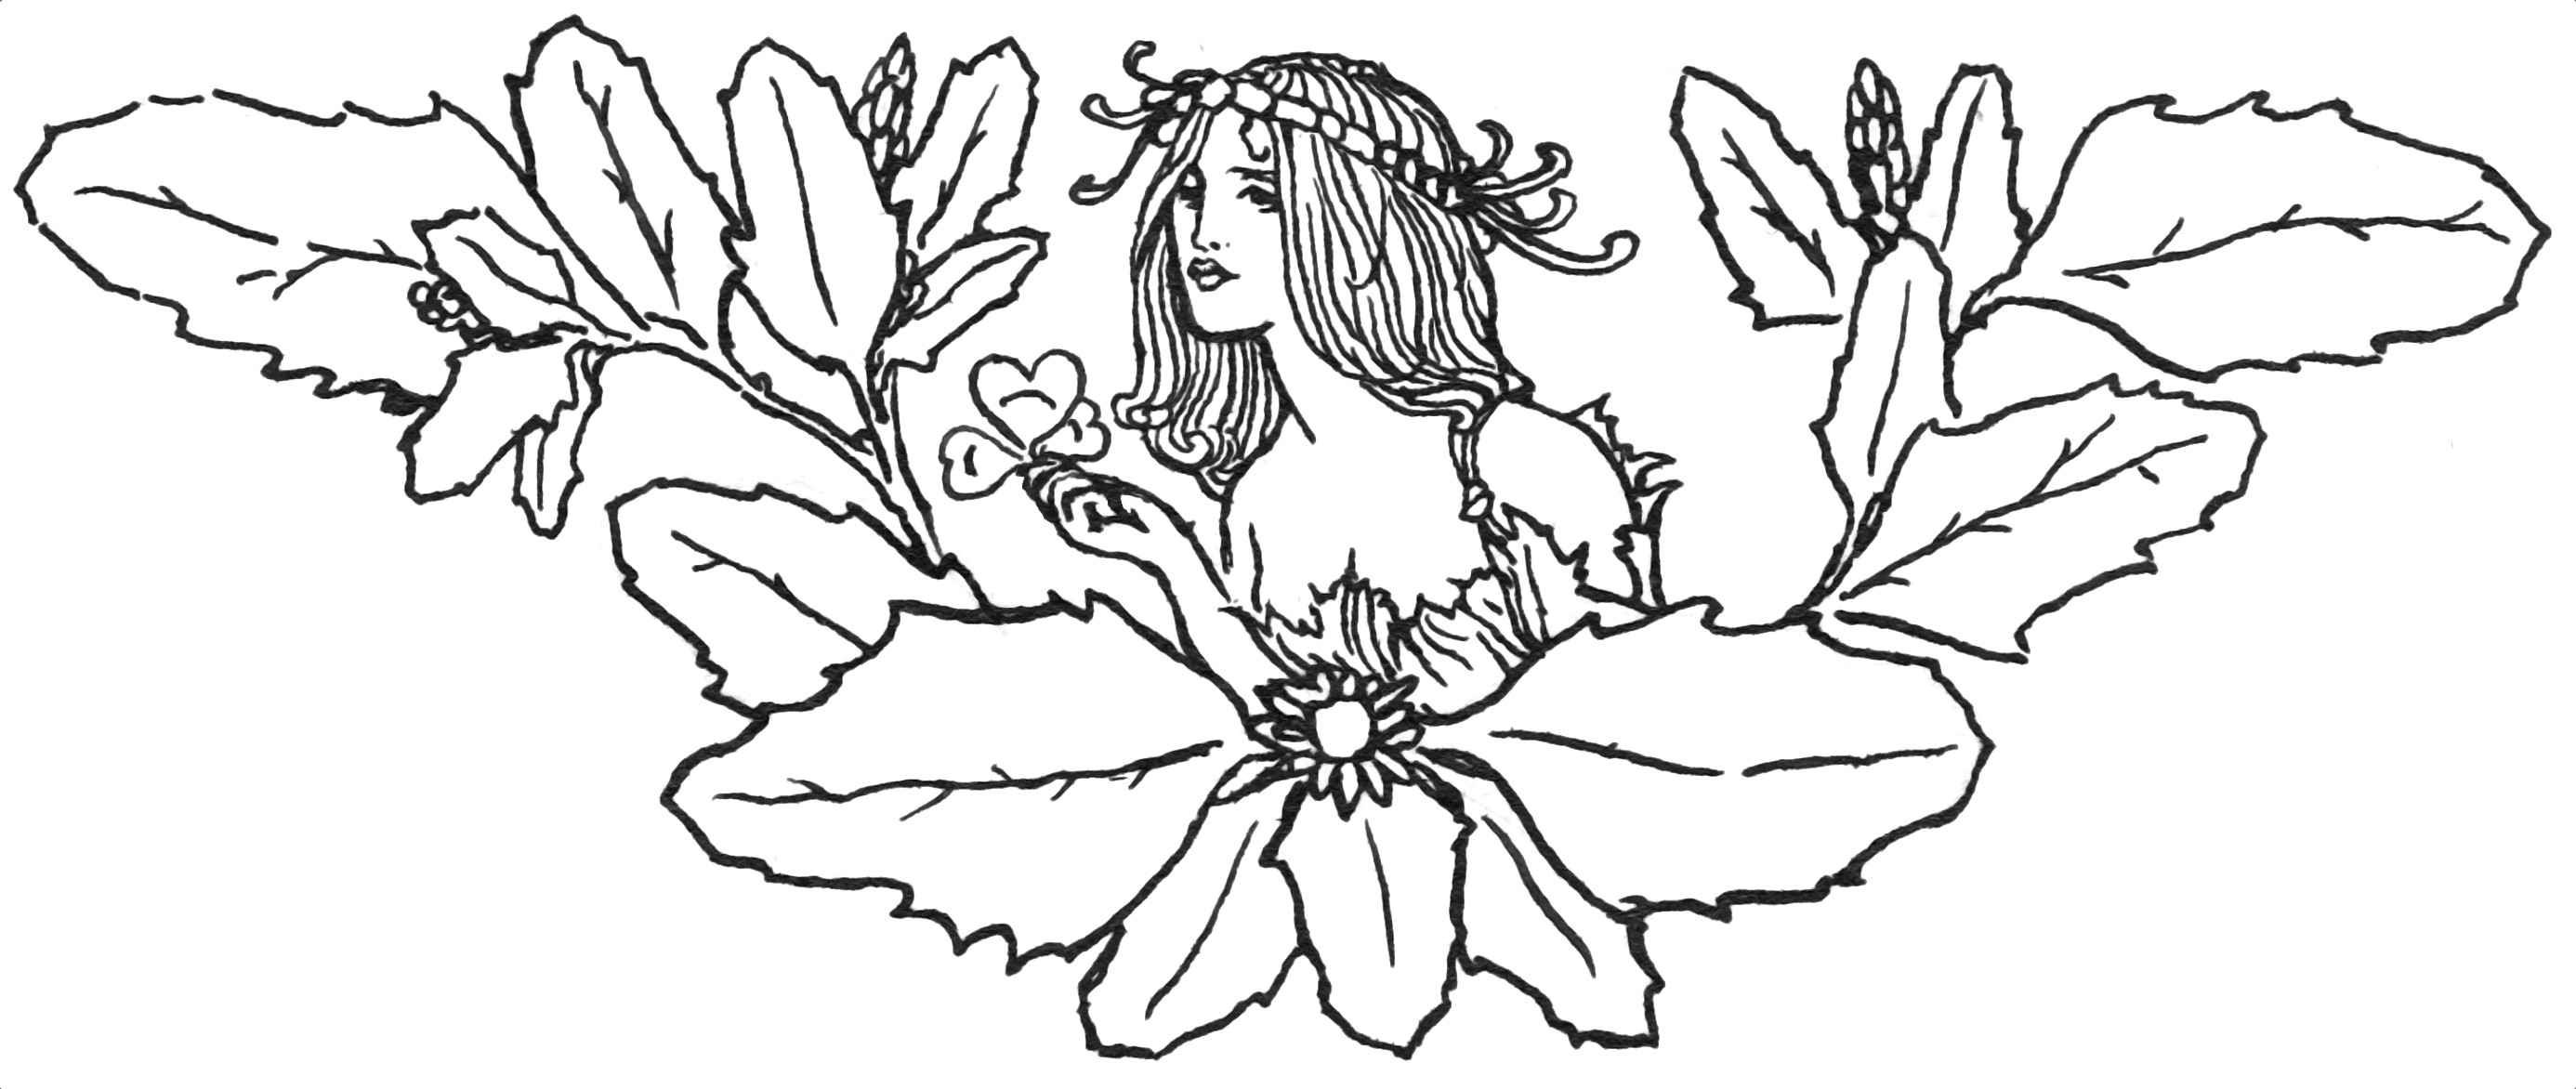
\includegraphics[width=\headerwidth]{1iiflowertail2}
\end{figure}


%end random decorations

\begin{verse_speech}[Prospero] 
\hspace{\widthof{The fraughting souls within her.}}Be collected:\\
No more amazement: tell your piteous heart\\
There's no harm done.\\
\end{verse_speech}

\verseline[Miranda]{\hspace{\widthof{There's no harm done.}}O, woe the day!}
	
\begin{verse_speech}[Prospero] 
\hspace{\widthof{There's no harm done. O, woe the day!}}No harm.\\
I have done nothing but in care of thee,\\
Of thee, my dear one, thee, my daughter, who\\
Art ignorant of what thou art, nought knowing\\
Of whence I am, nor that I am more better\\
Than Prospero, master of a full poor cell,\\
And thy no greater father.
\end{verse_speech}

\begin{pictures} % Miranda full-page portrait 1iimirandaportrait
	\begin{bwbigpic}
		[\picwidth]
		{1iimirandaportrait}
		{}
	\end{bwbigpic}
\end{pictures}

\begin{verse_speech}[Miranda] 
\hspace{\widthof{And thy no greater father.}}More to know\\
Did never meddle with my thoughts.
\end{verse_speech}

\begin{verse_speech}[Prospero] 
\hspace{\widthof{Did never meddle with my thoughts.}}'Tis time\\
I should inform thee farther. Lend thy hand,\\
And pluck my magic garment from me. So:\\
\stage{Lays down his mantle}
Lie there, my art. Wipe thou thine eyes; have comfort.\\
The direful spectacle of the wreck, which touch'd\\
The very virtue of compassion in thee,\\
I have with such provision in mine art\\
So safely ordered that there is no soul—\\
No, not so much perdition as an hair\\
Betid to any creature in the vessel\\
Which thou heard'st cry, which thou saw'st sink. Sit down;\\
For thou must now know farther.
\end{verse_speech}

\stage{They sit.}

\begin{figure}[b]
\centering

\includegraphics[width=\smallwidth]{1iilookright}
\end{figure}

\begin{verse_speech}[Miranda] 
\hspace{\widthof{For thou must now know farther.}}You have often\\
Begun to tell me what I am, but stopp'd\\
And left me to a bootless inquisition,\\
Concluding <Stay: not yet.>
\end{verse_speech}

\begin{verse_speech}[Prospero] 
\hspace{\widthof{Concluding <Stay: not yet.>}}The hour's now come;\\
The very minute bids thee ope thine ear;\\
Obey and be attentive. Canst thou remember\\
A time before we came unto this cell?\\
I do not think thou canst, for then thou wast not\\
Out three years old.
\end{verse_speech}

\verseline[Miranda]{\hspace{\widthof{Out three years old.}}Certainly, sir, I can.}
	
\begin{verse_speech}[Prospero] 
	By what? by any other house or person?\\
Of any thing the image tell me that\\
Hath kept with thy remembrance.
\end{verse_speech}

\begin{verse_speech}[Miranda] 
\hspace{\widthof{Hath kept with thy remembrance.}}'Tis far off\\
And rather like a dream than an assurance\\
That my remembrance warrants. Had I not\\
Four or five women once that tended me?
\end{verse_speech}

\begin{verse_speech}[Prospero] 
Thou hadst, and more, Miranda. But how is it\\
That this lives in thy mind? What seest thou else\\
In the dark backward and abysm of time?\\
If thou remember'st aught ere thou camest here,\\
How thou camest here thou mayst.
\end{verse_speech}

\verseline[Miranda]{\hspace{\widthof{How thou camest here thou mayst.}}But that I do not.}


\begin{pictures} %Miranda as a baby
	
\begin{bwbigpic}
	[\picwidth]
	{1iimirandababy}
	{}
\end{bwbigpic}
\end{pictures}


\begin{verse_speech}[Prospero] 
	Twelve year since, Miranda, twelve year since,\\
Thy father was the Duke of Milan and\\
A prince of power.
\end{verse_speech}

\verseline[Miranda]{\hspace{\widthof{A prince of power.}}Sir, are not you my father?}
	
\begin{verse_speech}[Prospero] 
Thy mother was a piece of virtue, and\\
She said thou wast my daughter; and thy father\\
Was Duke of Milan; and thou his only heir\\
And princess no worse issued.
\end{verse_speech}

\begin{verse_speech}[Miranda] 
\hspace{\widthof{And princess no worse issued.}}O the heavens!\\
What foul play had we, that we came from thence?\\
Or blessèd was't we did?
\end{verse_speech}

\begin{verse_speech}[Prospero] 
\hspace{\widthof{Or blessèd was't we did?}}Both, both, my girl:\\
By foul play, as thou say'st, were we heaved thence,\\
But blessedly holp hither.
\end{verse_speech}

\begin{verse_speech}[Miranda] 
\hspace{\widthof{But blessedly holp hither.}}O, my heart bleeds\\
To think o' the teen that I have turn'd you to,\\
Which is from my remembrance! Please you, farther.
\end{verse_speech}

\begin{verse_speech}[Prospero] 
My brother and thy uncle, call'd Antonio—\\
I pray thee, mark me—that a brother should\\
Be so perfidious!—he whom next thyself\\
Of all the world I loved and to him put\\
The manage of my state; as at that time\\
Through all the signories it was the first\\
And Prospero the prime duke, being so reputed\\
In dignity, and for the liberal arts\\
Without a parallel; those being all my study,\\
The government I cast upon my brother\\
And to my state grew stranger, being transported\\
And rapt in secret studies. Thy false uncle—\\
Dost thou attend me?
\end{verse_speech}

\verseline[Miranda]{\hspace{\widthof{Dost thou attend me?}}Sir, most heedfully.}
	
\begin{verse_speech}[Prospero] 
Being once perfected how to grant suits,\\
How to deny them, who to advance and who\\
To trash for over-topping, new created\\
The creatures that were mine, I say, or changed 'em,\\
Or else new form'd 'em; having both the key\\
Of officer and office, set all hearts i' the state\\
To what tune pleased his ear; that now he was\\
The ivy which had hid my princely trunk,\\
And suck'd my verdure out on't. Thou attend'st not.
\end{verse_speech}

\verseline[Miranda]{O, good sir, I do.}
	
\begin{verse_speech}[Prospero] 
\hspace{\widthof{O, good sir, I do.}}I pray thee, mark me.\\
I, thus neglecting worldly ends, all dedicated\\
To closeness and the bettering of my mind\\
With that which, but by being so retired,\\
O'er-prized all popular rate, in my false brother\\
Awaked an evil nature; and my trust,\\
Like a good parent, did beget of him\\
A falsehood in its contrary as great\\
As my trust was; which had indeed no limit,\\
A confidence sans bound. He being thus lorded,\\
Not only with what my revenue yielded,\\
But what my power might else exact, like one\\
Who having into truth, by telling of it,\\
Made such a sinner of his memory,\\
To credit his own lie, he did believe\\
He was indeed the duke; out o' the substitution\\
And executing the outward face of royalty,\\
With all prerogative: hence his ambition growing—\\
Dost thou hear?
\end{verse_speech}

\verseline[Miranda]{Your tale, sir, would cure deafness.}
	
\begin{verse_speech}[Prospero] 
To have no screen between this part he play'd\\
And him he play'd it for, he needs will be\\
Absolute Milan. Me, poor man, my library\\
Was dukedom large enough: of temporal royalties\\
He thinks me now incapable; confederates—\\
So dry he was for sway—wi' the King of Naples\\
To give him annual tribute, do him homage,\\
Subject his coronet to his crown and bend\\
The dukedom yet unbow'd—alas, poor Milan!—\\
To most ignoble stooping.
\end{verse_speech}

\verseline[Miranda]{\hspace{\widthof{To most ignoble stooping.}}O the heavens!}
	
\begin{verse_speech}[Prospero] 
Mark his condition and the event; then tell me\\
If this might be a brother.
\end{verse_speech}

\begin{verse_speech}[Miranda] 
\hspace{\widthof{If this might be a brother.}}I should sin\\
To think but nobly of my grandmother:\\
Good wombs have borne bad sons.
\end{verse_speech}

\begin{verse_speech}[Prospero] 
\hspace{\widthof{Good wombs have borne bad sons.}}Now the condition.\\
The King of Naples, being an enemy\\
To me inveterate, hearkens my brother's suit;\\
Which was, that he, in lieu o' the premises\\
Of homage and I know not how much tribute,\\
Should presently extirpate me and mine\\
Out of the dukedom and confer fair Milan\\
With all the honours on my brother: whereon,\\
A treacherous army levied, one midnight\\
Fated to the purpose did Antonio open\\
The gates of Milan, and, i' the dead of darkness,\\
The ministers for the purpose hurried thence\\
Me and thy crying self.
\end{verse_speech}

\begin{verse_speech}[Miranda] 
\hspace{\widthof{Me and thy crying self.}}Alack, for pity!\\
I, not remembering how I cried out then,\\
Will cry it o'er again: it is a hint\\
That wrings mine eyes to't.
\end{verse_speech}

\begin{verse_speech}[Prospero] 
\hspace{\widthof{That wrings mine eyes to't.}}Hear a little further\\
And then I'll bring thee to the present business\\
Which now's upon's; without the which this story\\
Were most impertinent.
\end{verse_speech}

\begin{verse_speech}[Miranda] 
\hspace{\widthof{Were most impertinent.}}Wherefore did they not\\
That hour destroy us?
\end{verse_speech}

\begin{verse_speech}[Prospero] 
\hspace{\widthof{That hour destroy us?}}Well demanded, wench:\\
My tale provokes that question. Dear, they durst not,\\
So dear the love my people bore me, nor set\\
A mark so bloody on the business, but\\
With colours fairer painted their foul ends.\\
In few, they hurried us aboard a bark,\\
Bore us some leagues to sea; where they prepared\\
A rotten carcass of a boat, not rigg'd,\\
Nor tackle, sail, nor mast; the very rats\\
Instinctively had quit it: there they hoist us,\\
To cry to the sea that roar'd to us, to sigh\\
To the winds whose pity, sighing back again,\\
Did us but loving wrong.
\end{verse_speech}

\begin{verse_speech}[Miranda] 
\hspace{\widthof{That hour destroy us?}}Alack, what trouble\\
Was I then to you!
\end{verse_speech}

\begin{verse_speech}[Prospero] 
\hspace{\widthof{Was I then to you!}}O, a cherubim\\
Thou wast that did preserve me. Thou didst smile.\\
Infusèd with a fortitude from heaven,\\
When I have deck'd the sea with drops full salt,\\
Under my burthen groan'd; which raised in me\\
An undergoing stomach, to bear up\\
Against what should ensue.
\end{verse_speech}

\verseline[Miranda]{How came we ashore?}
	
\begin{verse_speech}[Prospero] 
By Providence divine.\\
Some food we had and some fresh water that\\
A noble Neapolitan, Gonzalo,\\
Out of his charity, being then appointed\\
Master of this design, did give us, with\\
Rich garments, linens, stuffs and necessaries,\\
Which since have steaded much; so, of his gentleness,\\
Knowing I loved my books, he furnish'd me\\
From mine own library with volumes that\\
I prize above my dukedom.
\end{verse_speech}

\begin{verse_speech}[Miranda] 
\hspace{\widthof{I prize above my dukedom.}}Would I might\\
But ever see that man!
\end{verse_speech}

\begin{verse_speech}[Prospero] 
\hspace{\widthof{But ever see that man!}}Now I arise:\\
\stage{Stands and resumes his mantle}
Sit still, and hear the last of our sea-sorrow.\\
Here in this island we arrived; and here\\
Have I, thy schoolmaster, made thee more profit\\
Than other princesses can that have more time\\
For vainer hours and tutors not so careful.
\end{verse_speech}

\begin{verse_speech}[Miranda] 
Heavens thank you for't! And now, I pray you, sir,\\
For still 'tis beating in my mind, your reason\\
For raising this sea-storm?
\end{verse_speech}

\begin{verse_speech}[Prospero] 
\hspace{\widthof{For raising this sea-storm?}}Know thus far forth.\\
By accident most strange, bountiful Fortune,\\
Now my dear lady, hath mine enemies\\
Brought to this shore; and by my prescience\\
I find my zenith doth depend upon\\
A most auspicious star, whose influence\\
If now I court not but omit, my fortunes\\
Will ever after droop. Here cease more questions:\\
Thou art inclined to sleep; 'tis a good dullness,\\
And give it way: I know thou canst not choose.\\
\stage{\textsc{Miranda} sleeps}
Come away, servant, come. I am ready now.\\
Approach, my Ariel, come.\\
\end{verse_speech}
\enter{\textsc{Ariel}}

\begin{verse_speech}[Ariel] 
All hail, great master! grave sir, hail! I come\\
To answer thy best pleasure; be't to fly,\\
To swim, to dive into the fire, to ride\\
On the curl'd clouds, to thy strong bidding task\\
Ariel and all his quality.
\end{verse_speech}

\begin{figure}[tbh]
\centering
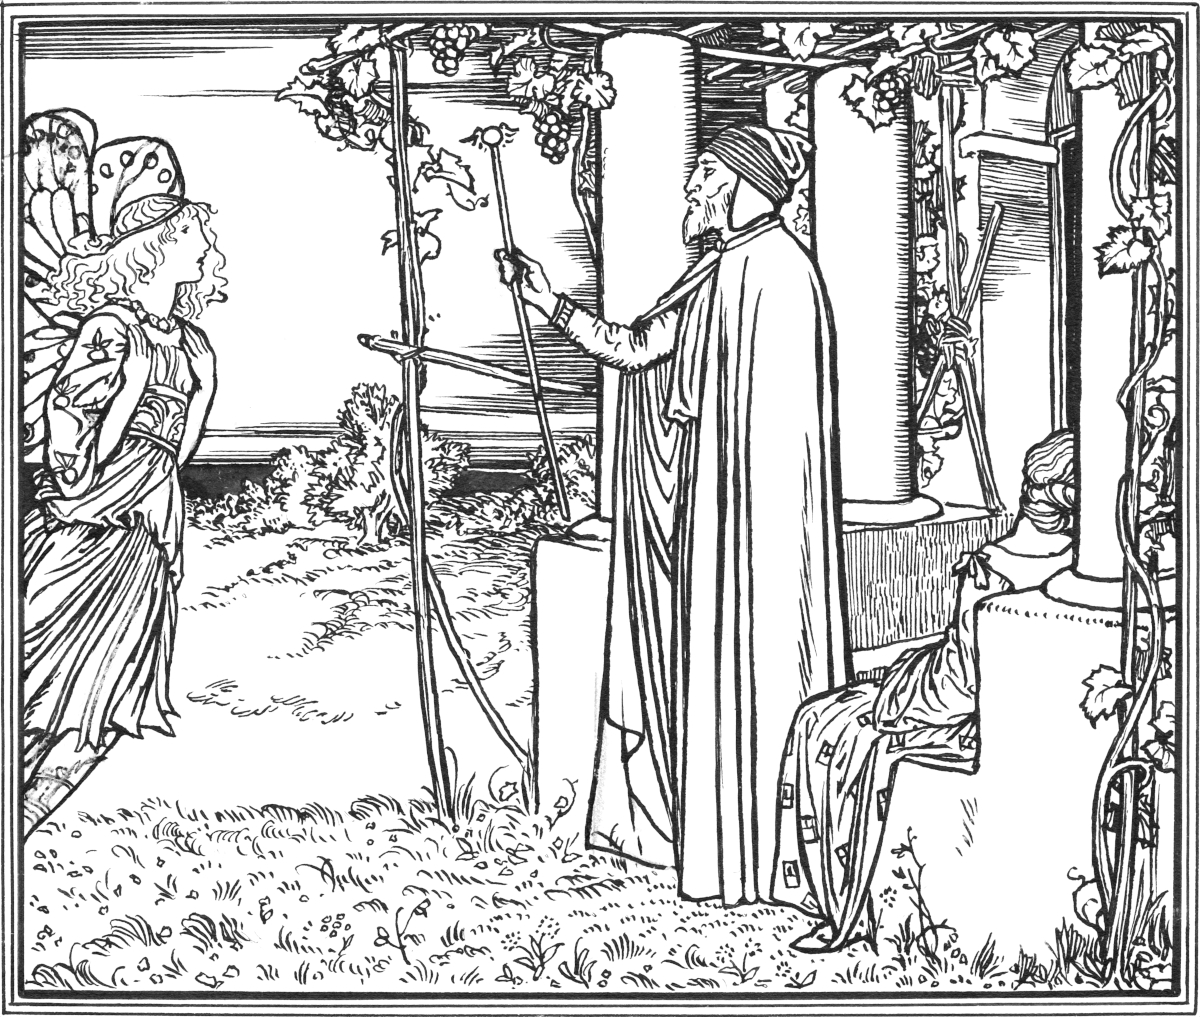
\includegraphics[width=\headerwidth]{1iiprosperoariel}
\end{figure}

\begin{verse_speech}[Prospero] 
\hspace{\widthof{Ariel and all his quality.}}Hast thou, spirit,\\
Perform'd to point the tempest that I bade thee?
\end{verse_speech}

\begin{verse_speech}[Ariel] 
To every article.\\
I boarded the king's ship; now on the beak,\\
Now in the waist, the deck, in every cabin,\\
I flamed amazement: sometime I'ld divide,\\
And burn in many places; on the topmast,\\
The yards and bowsprit, would I flame distinctly,\\
Then meet and join. Jove's lightnings, the precursors\\
O' the dreadful thunder-claps, more momentary\\
And sight-outrunning were not; the fire and cracks\\
Of sulphurous roaring the most mighty Neptune\\
Seem to besiege and make his bold waves tremble,\\
Yea, his dread trident shake.
\end{verse_speech}

\begin{verse_speech}[Prospero] 
\hspace{\widthof{Yea, his dread trident shake.}}My brave spirit!\\
Who was so firm, so constant, that this coil\\
Would not infect his reason?
\end{verse_speech}

\begin{verse_speech}[Ariel] 
\hspace{\widthof{Would not infect his reason?}}Not a soul\\
But felt a fever of the mad and play'd\\
Some tricks of desperation. All but mariners\\
Plunged in the foaming brine and quit the vessel,\\
Then all afire with me: the king's son, Ferdinand,\\
With hair up-staring,—then like reeds, not hair,—\\
Was the first man that leap'd; cried, <Hell is empty\\
And all the devils are here.>
\end{verse_speech}

\begin{verse_speech}[Prospero] 
\hspace{\widthof{And all the devils are here.}}Why that's my spirit!\\
But was not this nigh shore?
\end{verse_speech}

\verseline[Ariel]{\hspace{\widthof{But was not this nigh shore?}}Close by, my master.}
	
\verseline[Prospero]{But are they, Ariel, safe?}
	
\begin{verse_speech}[Ariel] 
\hspace{\widthof{But are they, Ariel, safe?}}Not a hair perish'd;\\
On their sustaining garments not a blemish,\\
But fresher than before: and, as thou badest me,\\
In troops I have dispersed them 'bout the isle.\\
The king's son have I landed by himself;\\
Whom I left cooling of the air with sighs\\
In an odd angle of the isle and sitting,\\
His arms in this sad knot.
\end{verse_speech}
\stage{He folds his arms.}

\begin{verse_speech}[Prospero] 
\hspace{\widthof{His arms in this sad knot.}}Of the king's ship\\
The mariners say how thou hast disposed\\
And all the rest o' the fleet.
\end{verse_speech}

\begin{verse_speech}[Ariel] 
\hspace{\widthof{And all the rest o' the fleet.}}Safely in harbour\\
Is the king's ship; in the deep nook, where once\\
Thou call'dst me up at midnight to fetch dew\\
From the still-vex'd Bermoothes, there she's hid:\\
The mariners all under hatches stow'd;\\
Who, with a charm join'd to their suffer'd labour,\\
I have left asleep; and for the rest o' the fleet\\
Which I dispersed, they all have met again\\
And are upon the Mediterranean flote,\\
Bound sadly home for Naples,\\
Supposing that they saw the king's ship wreck'd\\
And his great person perish.
\end{verse_speech}

\begin{verse_speech}[Prospero] 
\hspace{\widthof{And his great person perish.}}Ariel, thy charge\\
Exactly is perform'd: but there's more work.\\
What is the time o' the day?
\end{verse_speech}

\verseline[Ariel]{\hspace{\widthof{What is the time o' the day?}}Past the mid season.}


\begin{figure}[tbh]
\centering
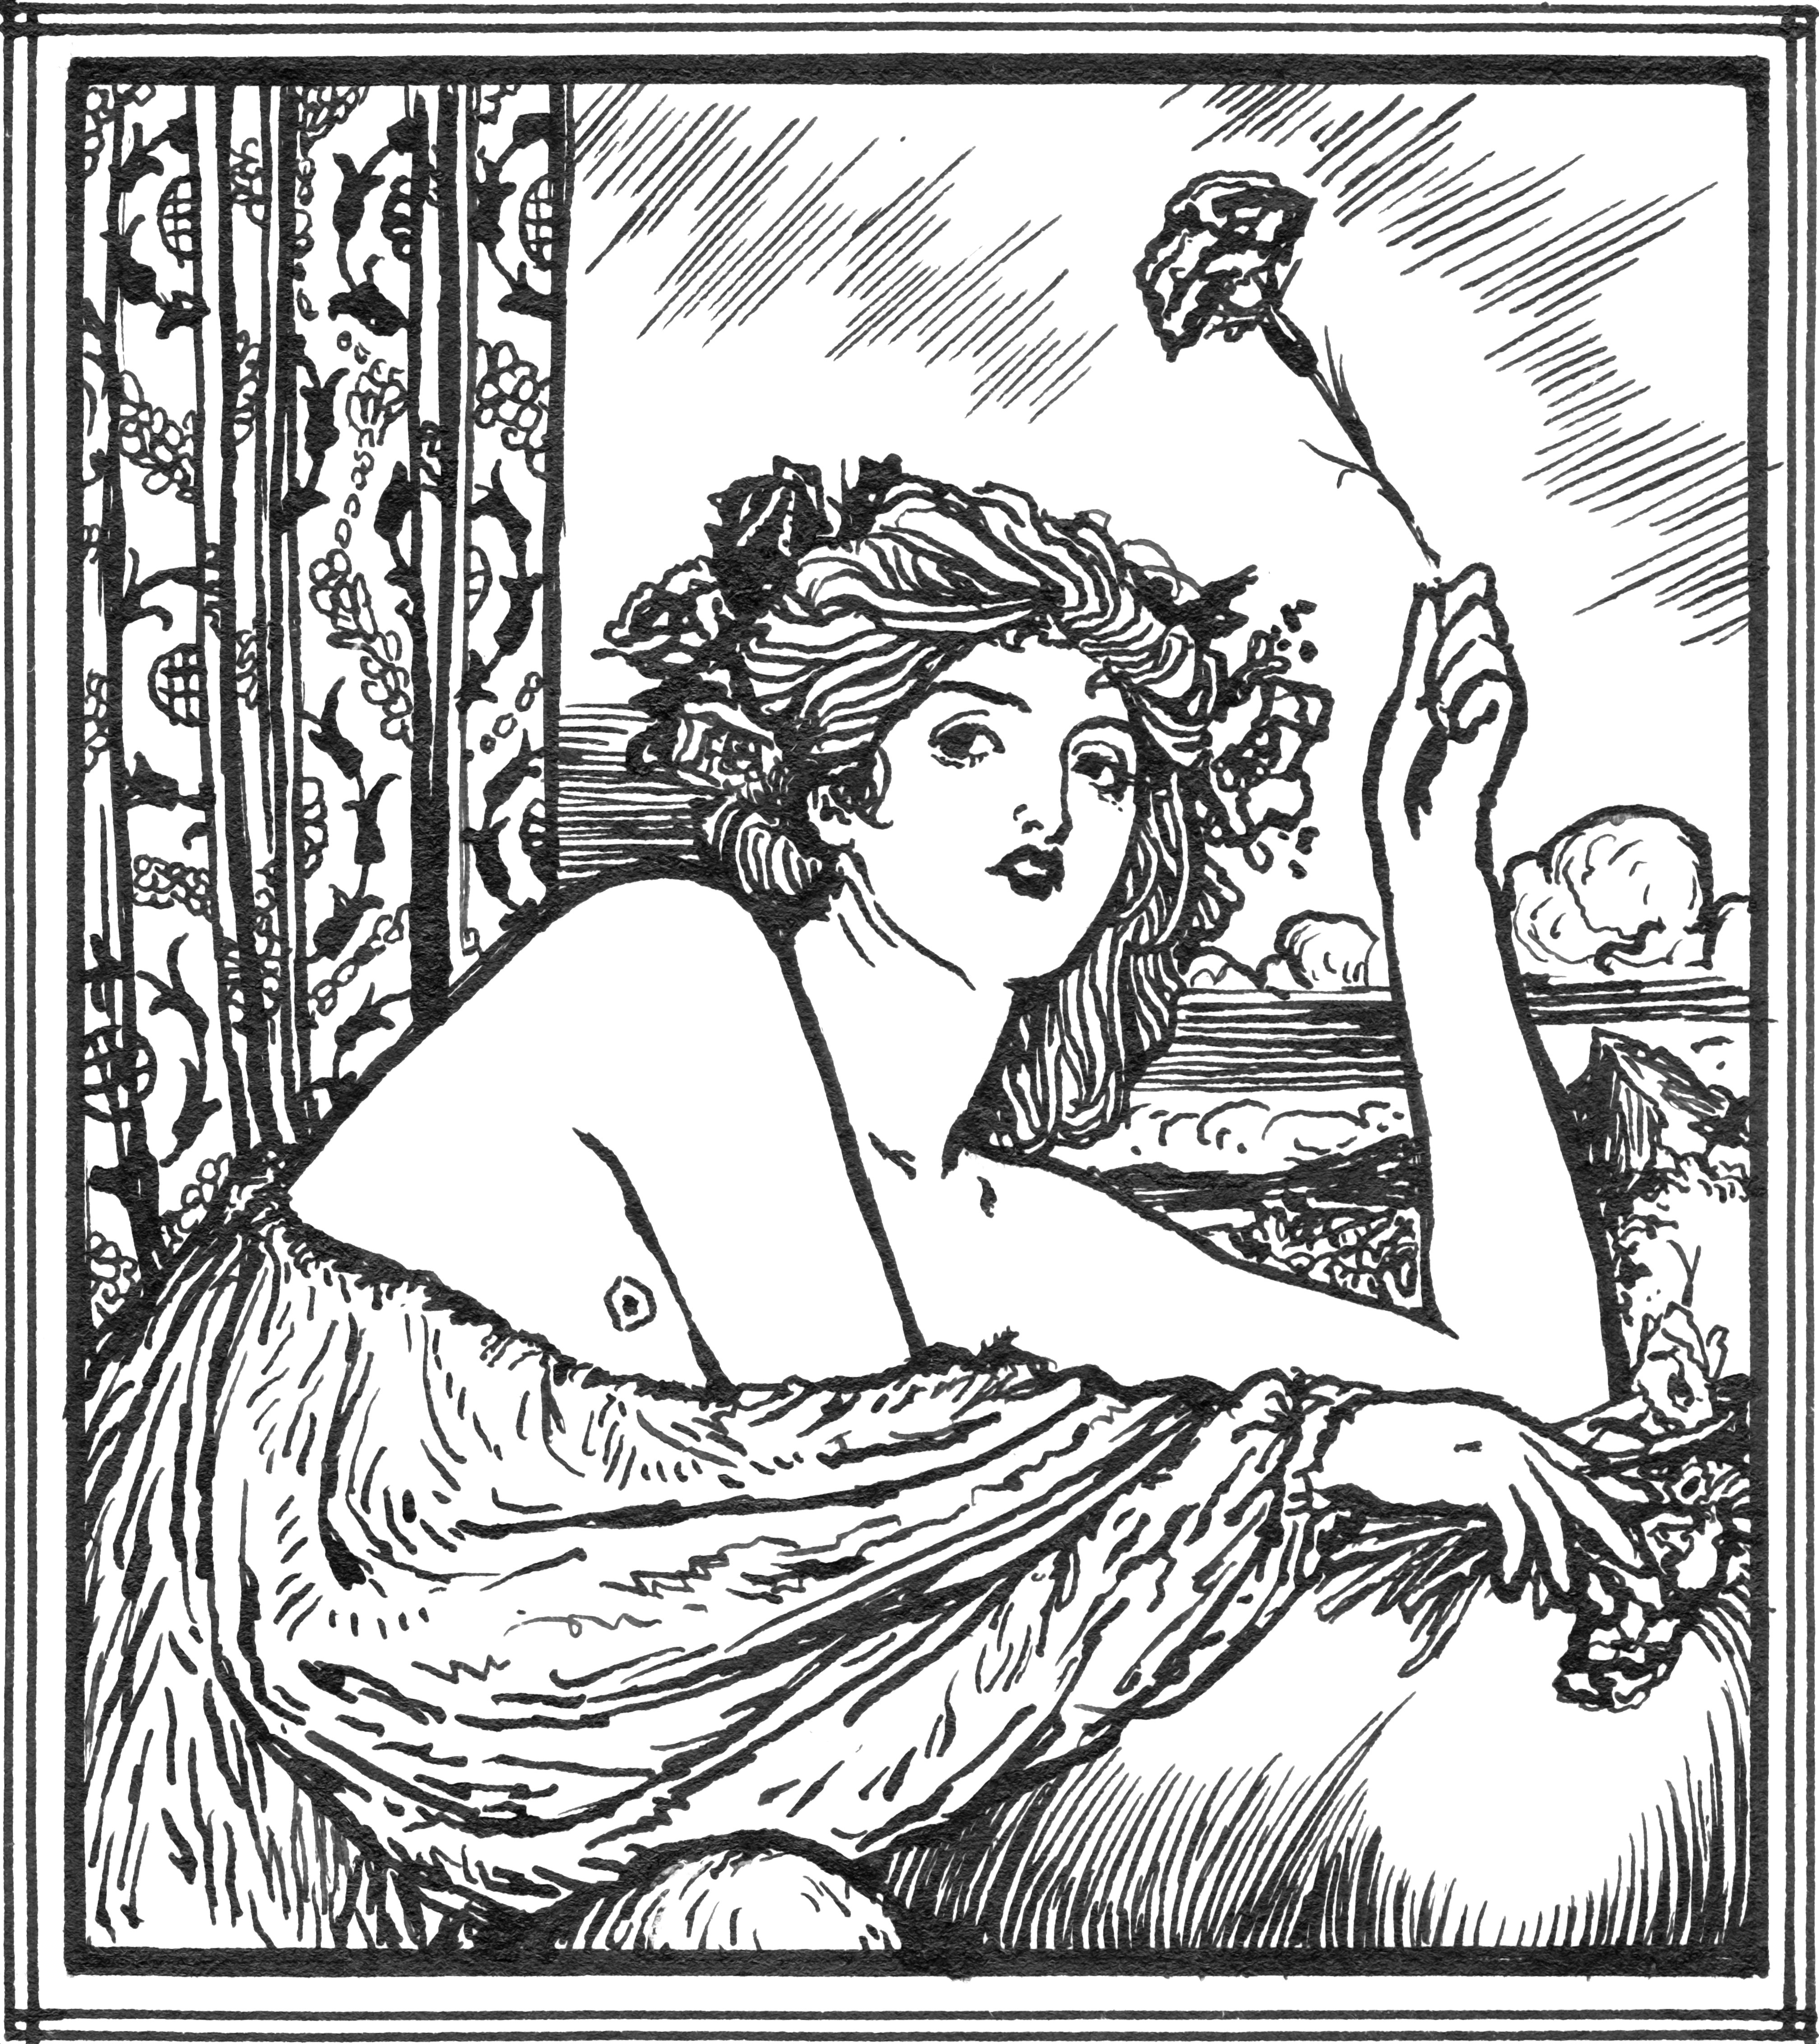
\includegraphics[width=.6\textwidth]{1iiflowerlady}
\end{figure}

\begin{verse_speech}[Prospero] 
At least two glasses. The time 'twixt six and now\\
Must by us both be spent most preciously.
\end{verse_speech}

\begin{verse_speech}[Ariel] 
Is there more toil? Since thou dost give me pains,\\
Let me remember thee what thou hast promised,
Which is not yet perform'd me.
\end{verse_speech}

\begin{verse_speech}[Prospero] 
\hspace{\widthof{Which is not yet perform'd me.}}How now? moody?\\
What is't thou canst demand?
\end{verse_speech}

\verseline[Ariel]{\hspace{\widthof{What is't thou canst demand?}}My liberty.}
	
\verseline[Prospero]{Before the time be out? no more!}
	
\begin{verse_speech}[Ariel] 
\hspace{\widthof{Before the time be out? no more!}}I prithee,\\
Remember I have done thee worthy service;\\
Told thee no lies, made thee no mistakings, served\\
Without or grudge or grumblings: thou didst promise\\
To bate me a full year.
\end{verse_speech}

\begin{verse_speech}[Prospero] 
\hspace{\widthof{To bate me a full year.}}Dost thou forget\\
From what a torment I did free thee?
\end{verse_speech}

\verseline[Ariel]{\hspace{\widthof{From what a torment I did free thee?}}No.}
	

\begin{pictures} %Ariel leans on a tree and looks moody
\begin{bwbigpic}
	[\picwidth]
	{1iiarieltree}
	{}
\end{bwbigpic}

\end{pictures}



\begin{verse_speech}[Prospero] 
Thou dost, and think'st it much to tread the ooze\\
Of the salt deep,\\
To run upon the sharp wind of the north,\\
To do me business in the veins o' the earth\\
When it is baked with frost.
\end{verse_speech}

\verseline[Ariel]{\hspace{\widthof{When it is baked with frost.}}I do not, sir.}

\begin{verse_speech}[Prospero] 
Thou liest, malignant thing! Hast thou forgot\\
The foul witch Sycorax, who with age and envy\\
Was grown into a hoop? hast thou forgot her?
\end{verse_speech}

\verseline[Ariel]{No, sir.}
	
\verseline[Prospero]{Thou hast. Where was she born? speak; tell me.}
	
\verseline[Ariel]{Sir, in Argier.}
	
\begin{verse_speech}[Prospero] 
\hspace{\widthof{Sir, in Argier.}}O, was she so? I must\\
Once in a month recount what thou hast been,\\
Which thou forget'st. This damn'd witch Sycorax,\\
For mischiefs manifold and sorceries terrible\\
To enter human hearing, from Argier,\\
Thou know'st, was banish'd: for one thing she did\\
They would not take her life. Is not this true?
\end{verse_speech}

\verseline[Ariel]{Ay, sir.}
	
\begin{verse_speech}[Prospero] 
This blue-eyed hag was hither brought with child\\
And here was left by the sailors. Thou, my slave,\\
As thou report'st thyself, wast then her servant;\\
And, for thou wast a spirit too delicate\\
To act her earthy and abhorr'd commands,\\
Refusing her grand hests, she did confine thee,\\
By help of her more potent ministers\\
And in her most unmitigable rage,\\
Into a cloven pine; within which rift\\
Imprison'd thou didst painfully remain\\
A dozen years; within which space she died\\
And left thee there; where thou didst vent thy groans\\
As fast as mill-wheels strike. Then was this island—\\
Save for the son that she did litter here,\\
A freckled whelp hag-born—not honour'd with\\
A human shape.
\end{verse_speech}

\verseline[Ariel]{\hspace{\widthof{A human shape.}}Yes, Caliban her son.}
	
\begin{verse_speech}[Prospero] 
Dull thing, I say so; he, that Caliban\\
Whom now I keep in service. Thou best know'st\\
What torment I did find thee in; thy groans\\
Did make wolves howl and penetrate the breasts\\
Of ever angry bears: it was a torment\\
To lay upon the damn'd, which Sycorax\\
Could not again undo: it was mine art,\\
When I arrived and heard thee, that made gape\\
The pine and let thee out.
\end{verse_speech}

\verseline[Ariel]{\hspace{\widthof{The pine and let thee out.}}I thank thee, master.}
	
\begin{verse_speech}[Prospero] 
If thou more murmur'st, I will rend an oak\\
And peg thee in his knotty entrails till\\
Thou hast howl'd away twelve winters.
\end{verse_speech}

\begin{verse_speech}[Ariel] 
\hspace{\widthof{Thou hast howl'd away twelve winters.}}Pardon, master;\\
I will be correspondent to command\\
And do my spiriting gently.
\end{verse_speech}

\begin{figure}[tbh]
\centering
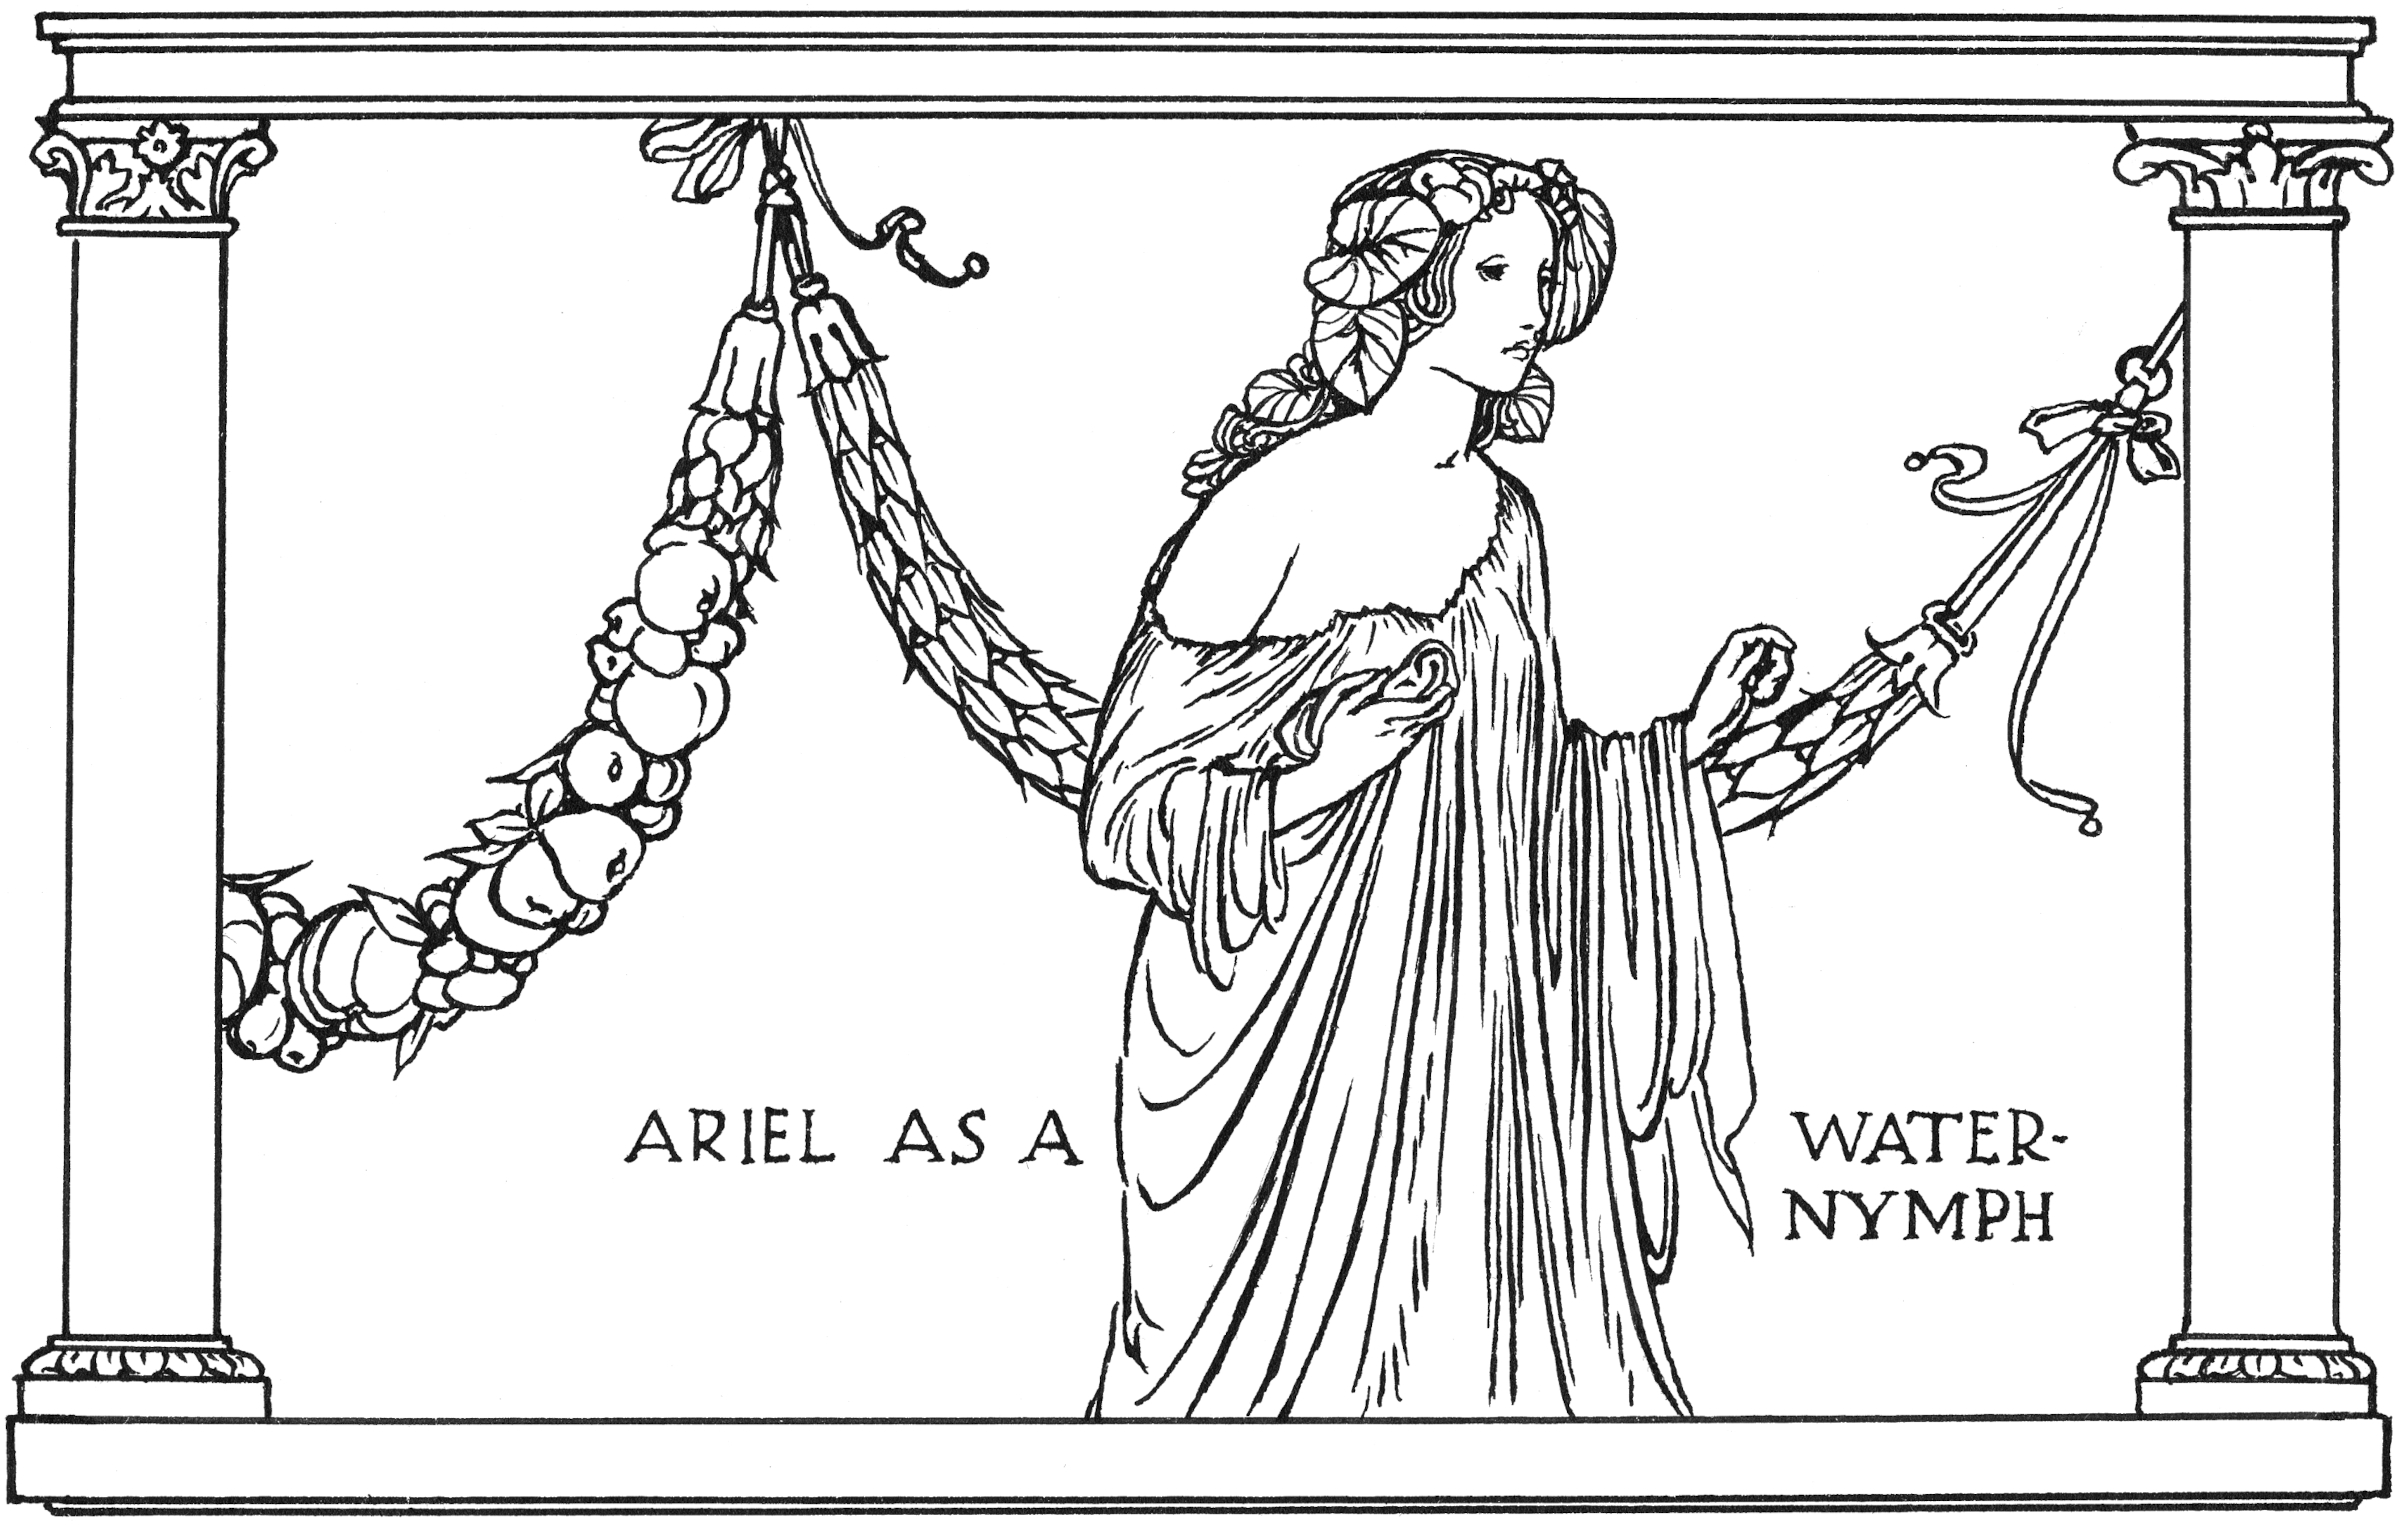
\includegraphics[width=\headerwidth]{1iiarielwaternymph}
\end{figure}

\begin{verse_speech}[Prospero] 
\hspace{\widthof{And do my spiriting gently.}}Do so, and after two days\\
I will discharge thee.
\end{verse_speech}

\begin{verse_speech}[Ariel] 
\hspace{\widthof{I will discharge thee.}}That's my noble master!\\
What shall I do? say what; what shall I do?
\end{verse_speech}

\begin{verse_speech}[Prospero] 
Go make thyself like a nymph o' the sea: be subject\\
To no sight but thine and mine, invisible\\
To every eyeball else. Go take this shape\\
And hither come in't: go, hence with diligence!\\
\exit{\textsc{Ariel}}
Awake, dear heart, awake! thou hast slept well; \\
Awake!
\end{verse_speech}

\begin{verse_speech}[Miranda] 
\hspace{\widthof{Awake!}}The strangeness of your story put\\
Heaviness in me.
\end{verse_speech}

\begin{verse_speech}[Prospero] 
\hspace{\widthof{Heaviness in me.}}Shake it off. Come on;\\
We'll visit Caliban my slave, who never\\
Yields us kind answer.
\end{verse_speech}

\begin{verse_speech}[Miranda] 
\hspace{\widthof{Yields us kind answer.}}'Tis a villain, sir,\\
I do not love to look on.
\end{verse_speech}

\begin{verse_speech}[Prospero] 
\hspace{\widthof{I do not love to look on.}}But, as 'tis,\\
We cannot miss him: he does make our fire,\\
Fetch in our wood and serves in offices\\
That profit us. What, ho! slave! Caliban!\\
Thou earth, thou! speak.
\end{verse_speech}

\verseline[Caliban]{\textit{[Within]} \hspace{\widthof{Thou earth, thou! speak.}}There's wood enough within.}

\begin{verse_speech}[Prospero] 
Come forth, I say! there's other business for thee:\\
Come, thou tortoise! when?\\
\stage{Re-enter \textsc{Ariel} like a water-nymph}
Fine apparition! My quaint Ariel,\\
Hark in thine ear.
\end{verse_speech}

\stage{He whispers to \textsc{Ariel}.}

\verseline[Ariel]{\hspace{\widthof{Hark in thine ear.}}My lord, it shall be done.}
\exit{}

\begin{verse_speech}[Prospero] 
Thou poisonous slave, got by the devil himself\\
Upon thy wicked dam, come forth!
\end{verse_speech}
\enter{\textsc{Caliban}}

\begin{figure}[tbh]
\centering
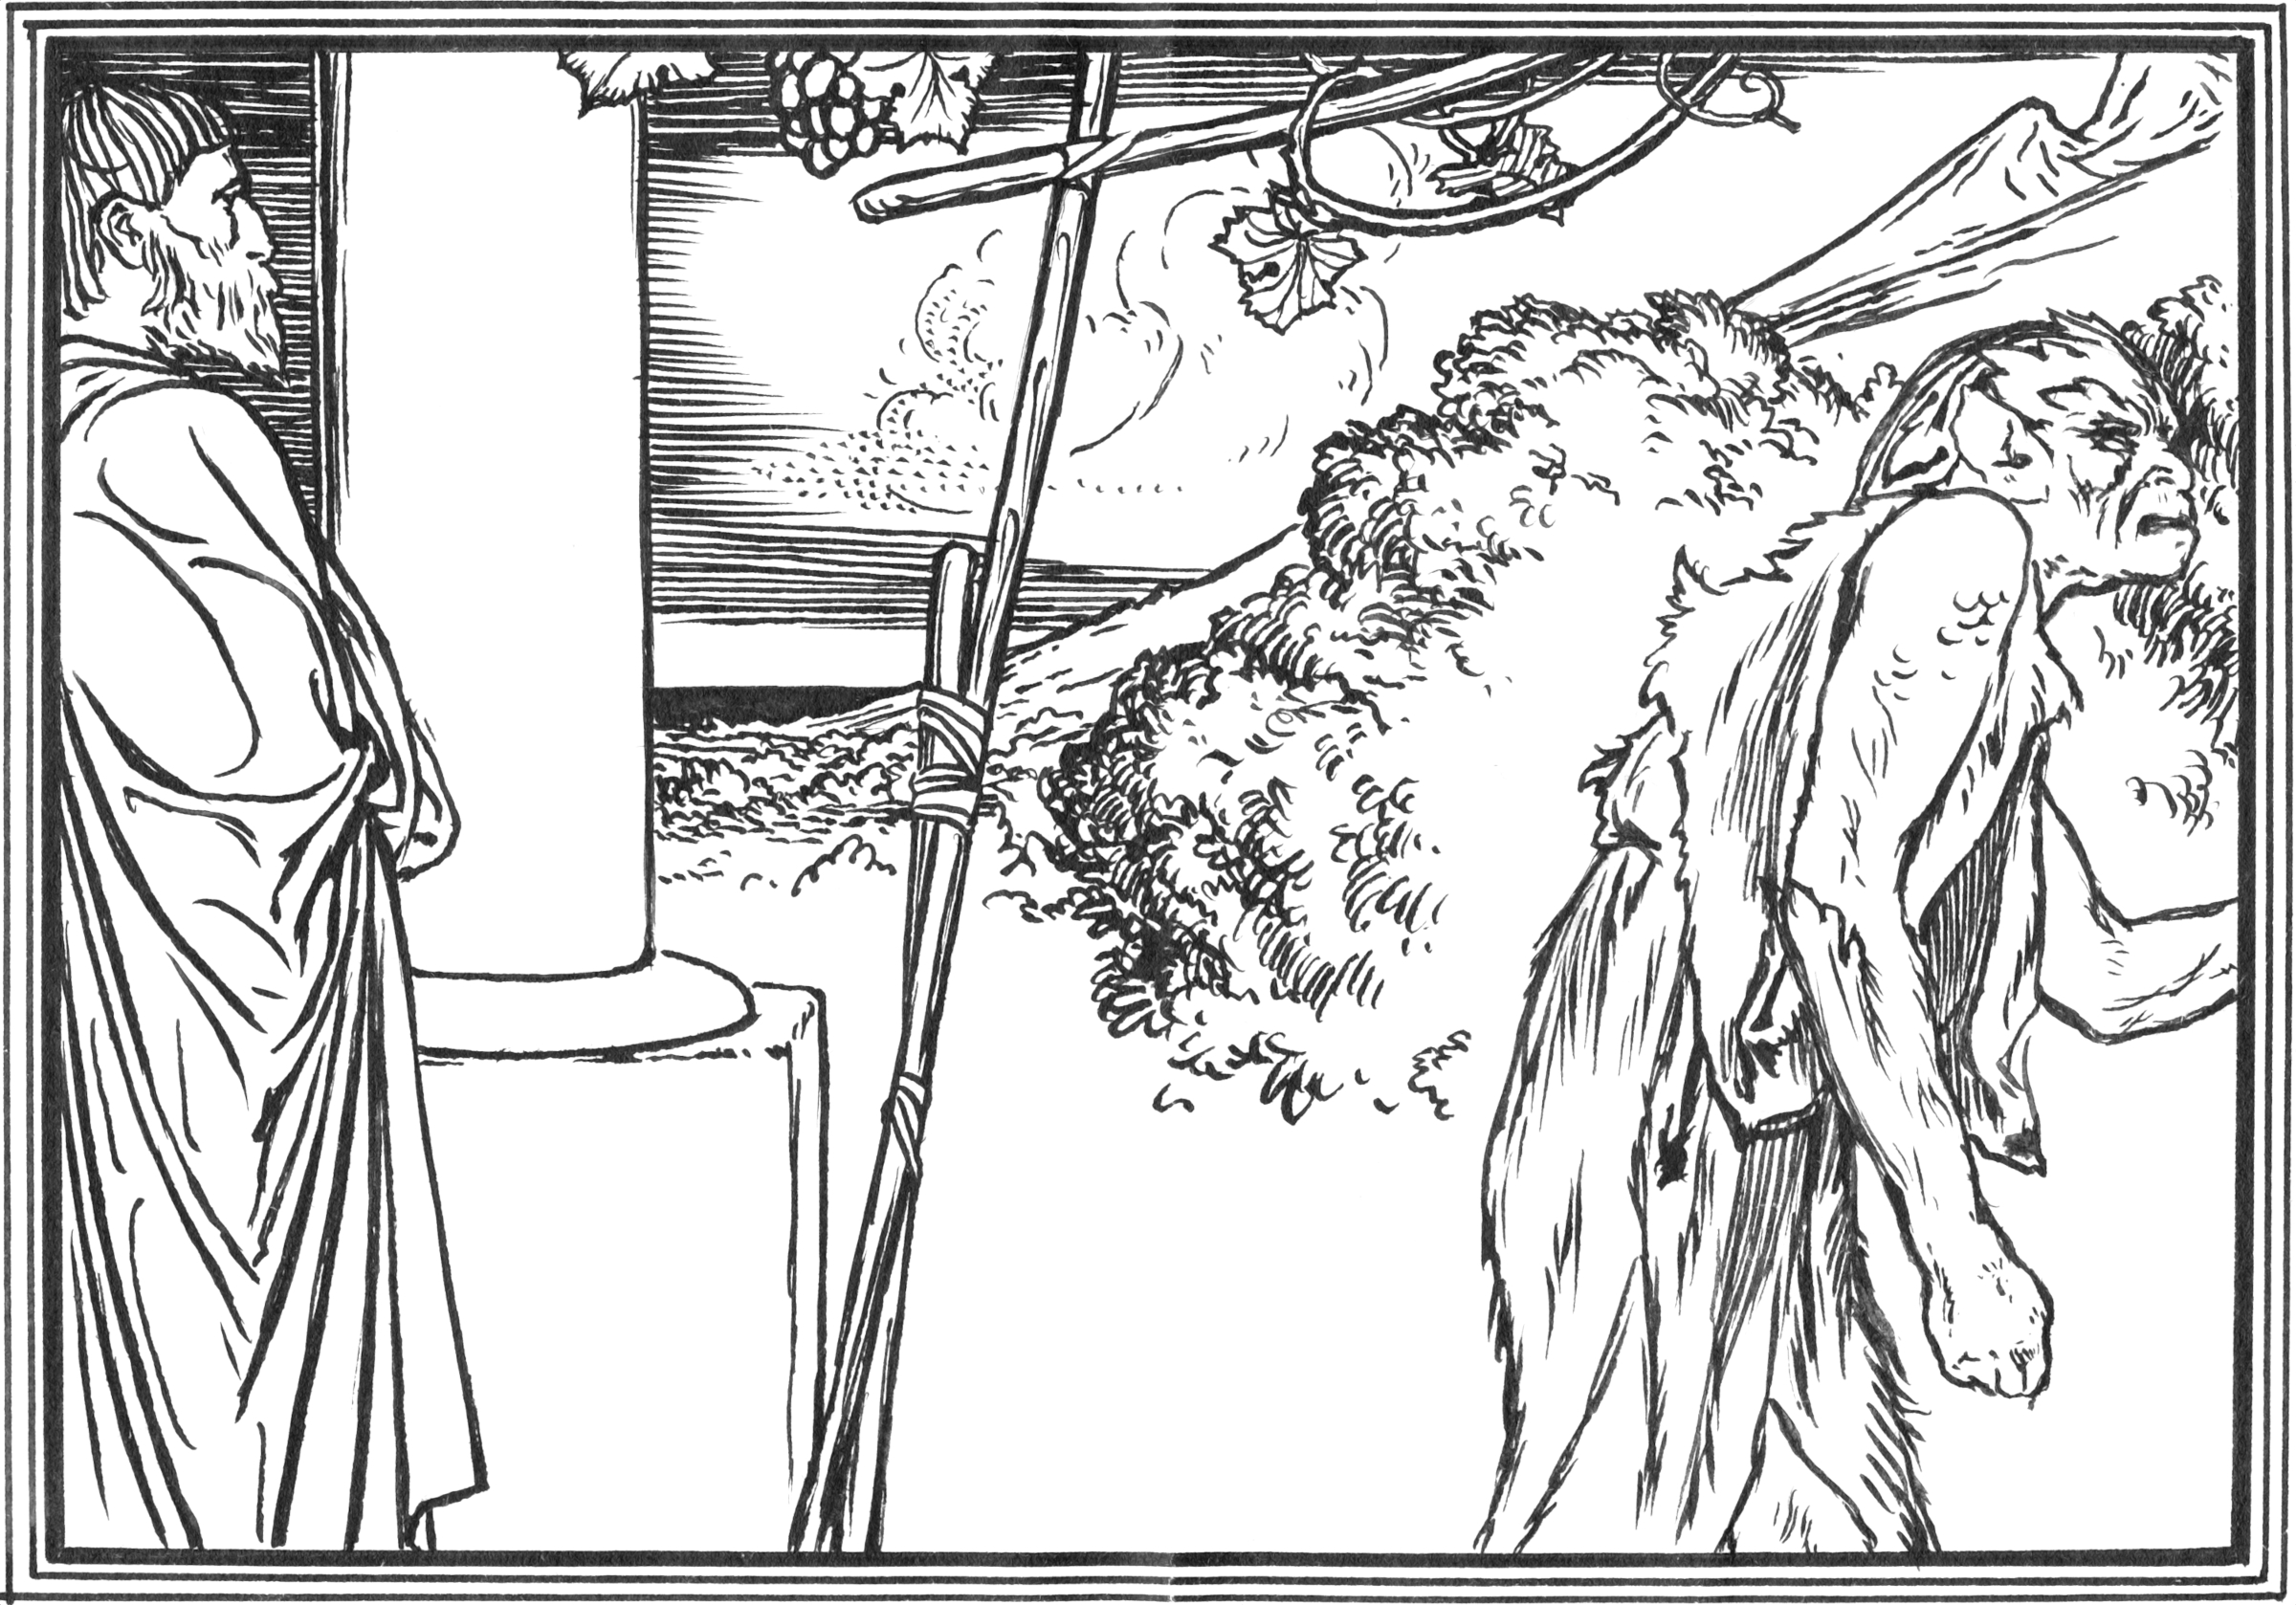
\includegraphics[width=\smallwidth]{1iicalibanprospero}
\end{figure}

\begin{figure}[tbh]
\centering
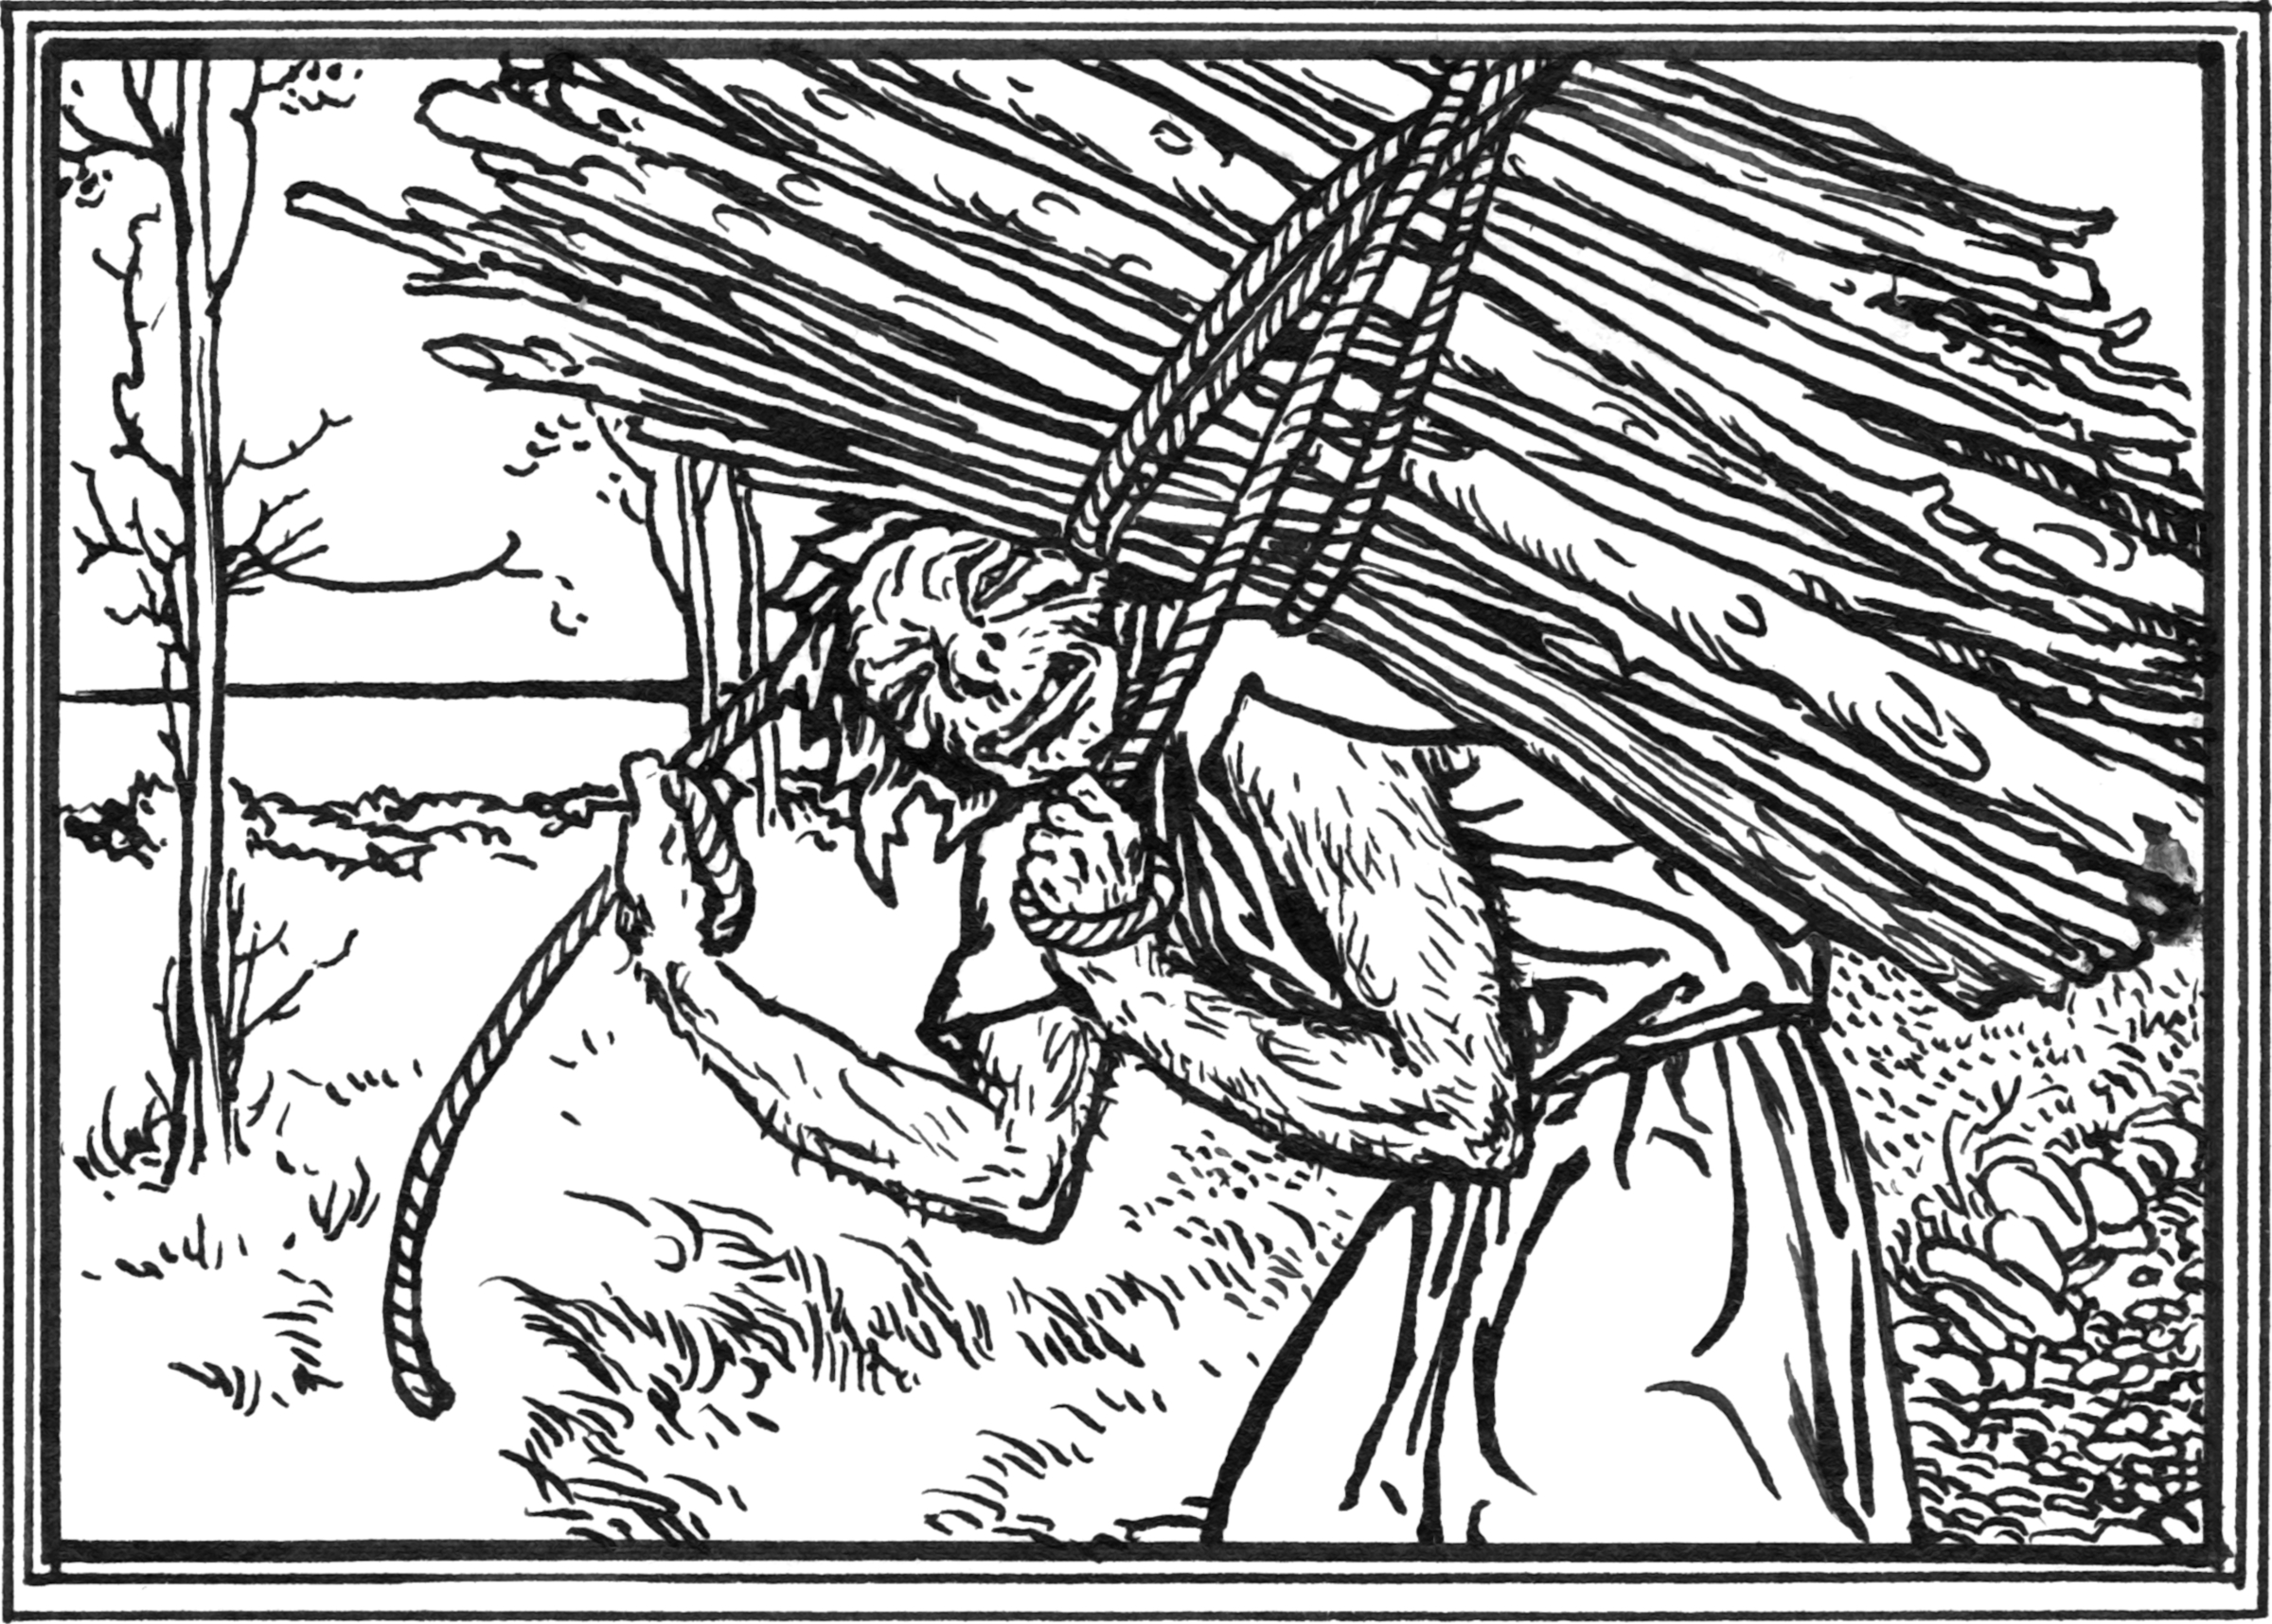
\includegraphics[width=\smallwidth]{1iicalibansticks}
\end{figure}

\begin{verse_speech}[Caliban] 
As wicked dew as e'er my mother brush'd\\
With raven's feather from unwholesome fen\\
Drop on you both! a south-west blow on ye\\
And blister you all o'er!
\end{verse_speech}

\begin{verse_speech}[Prospero] 
For this, be sure, to-night thou shalt have cramps,\\
Side-stitches that shall pen thy breath up; urchins\\
Shall, for that vast of night that they may work,\\
All exercise on thee; thou shalt be pinch'd\\
As thick as honeycomb, each pinch more stinging\\
Than bees that made 'em.
\end{verse_speech}

\begin{verse_speech}[Caliban] 
\hspace{\widthof{Than bees that made 'em.}}I must eat my dinner.\\
This island's mine, by Sycorax my mother,\\
Which thou takest from me. When thou camest first,\\
Thou strokedst me and madest much of me, wouldst give me\\
Water with berries in't, and teach me how\\
To name the bigger light, and how the less,\\
That burn by day and night: and then I loved thee\\
And show'd thee all the qualities o' the isle,\\
The fresh springs, brine-pits, barren place and fertile:\\
Cursed be I that did so! All the charms\\
Of Sycorax, toads, beetles, bats, light on you!\\
For I am all the subjects that you have,\\
Which first was mine own king: and here you sty me\\
In this hard rock, whiles you do keep from me\\
The rest o' the island.
\end{verse_speech}

\begin{figure}[tbh]
	\centering
	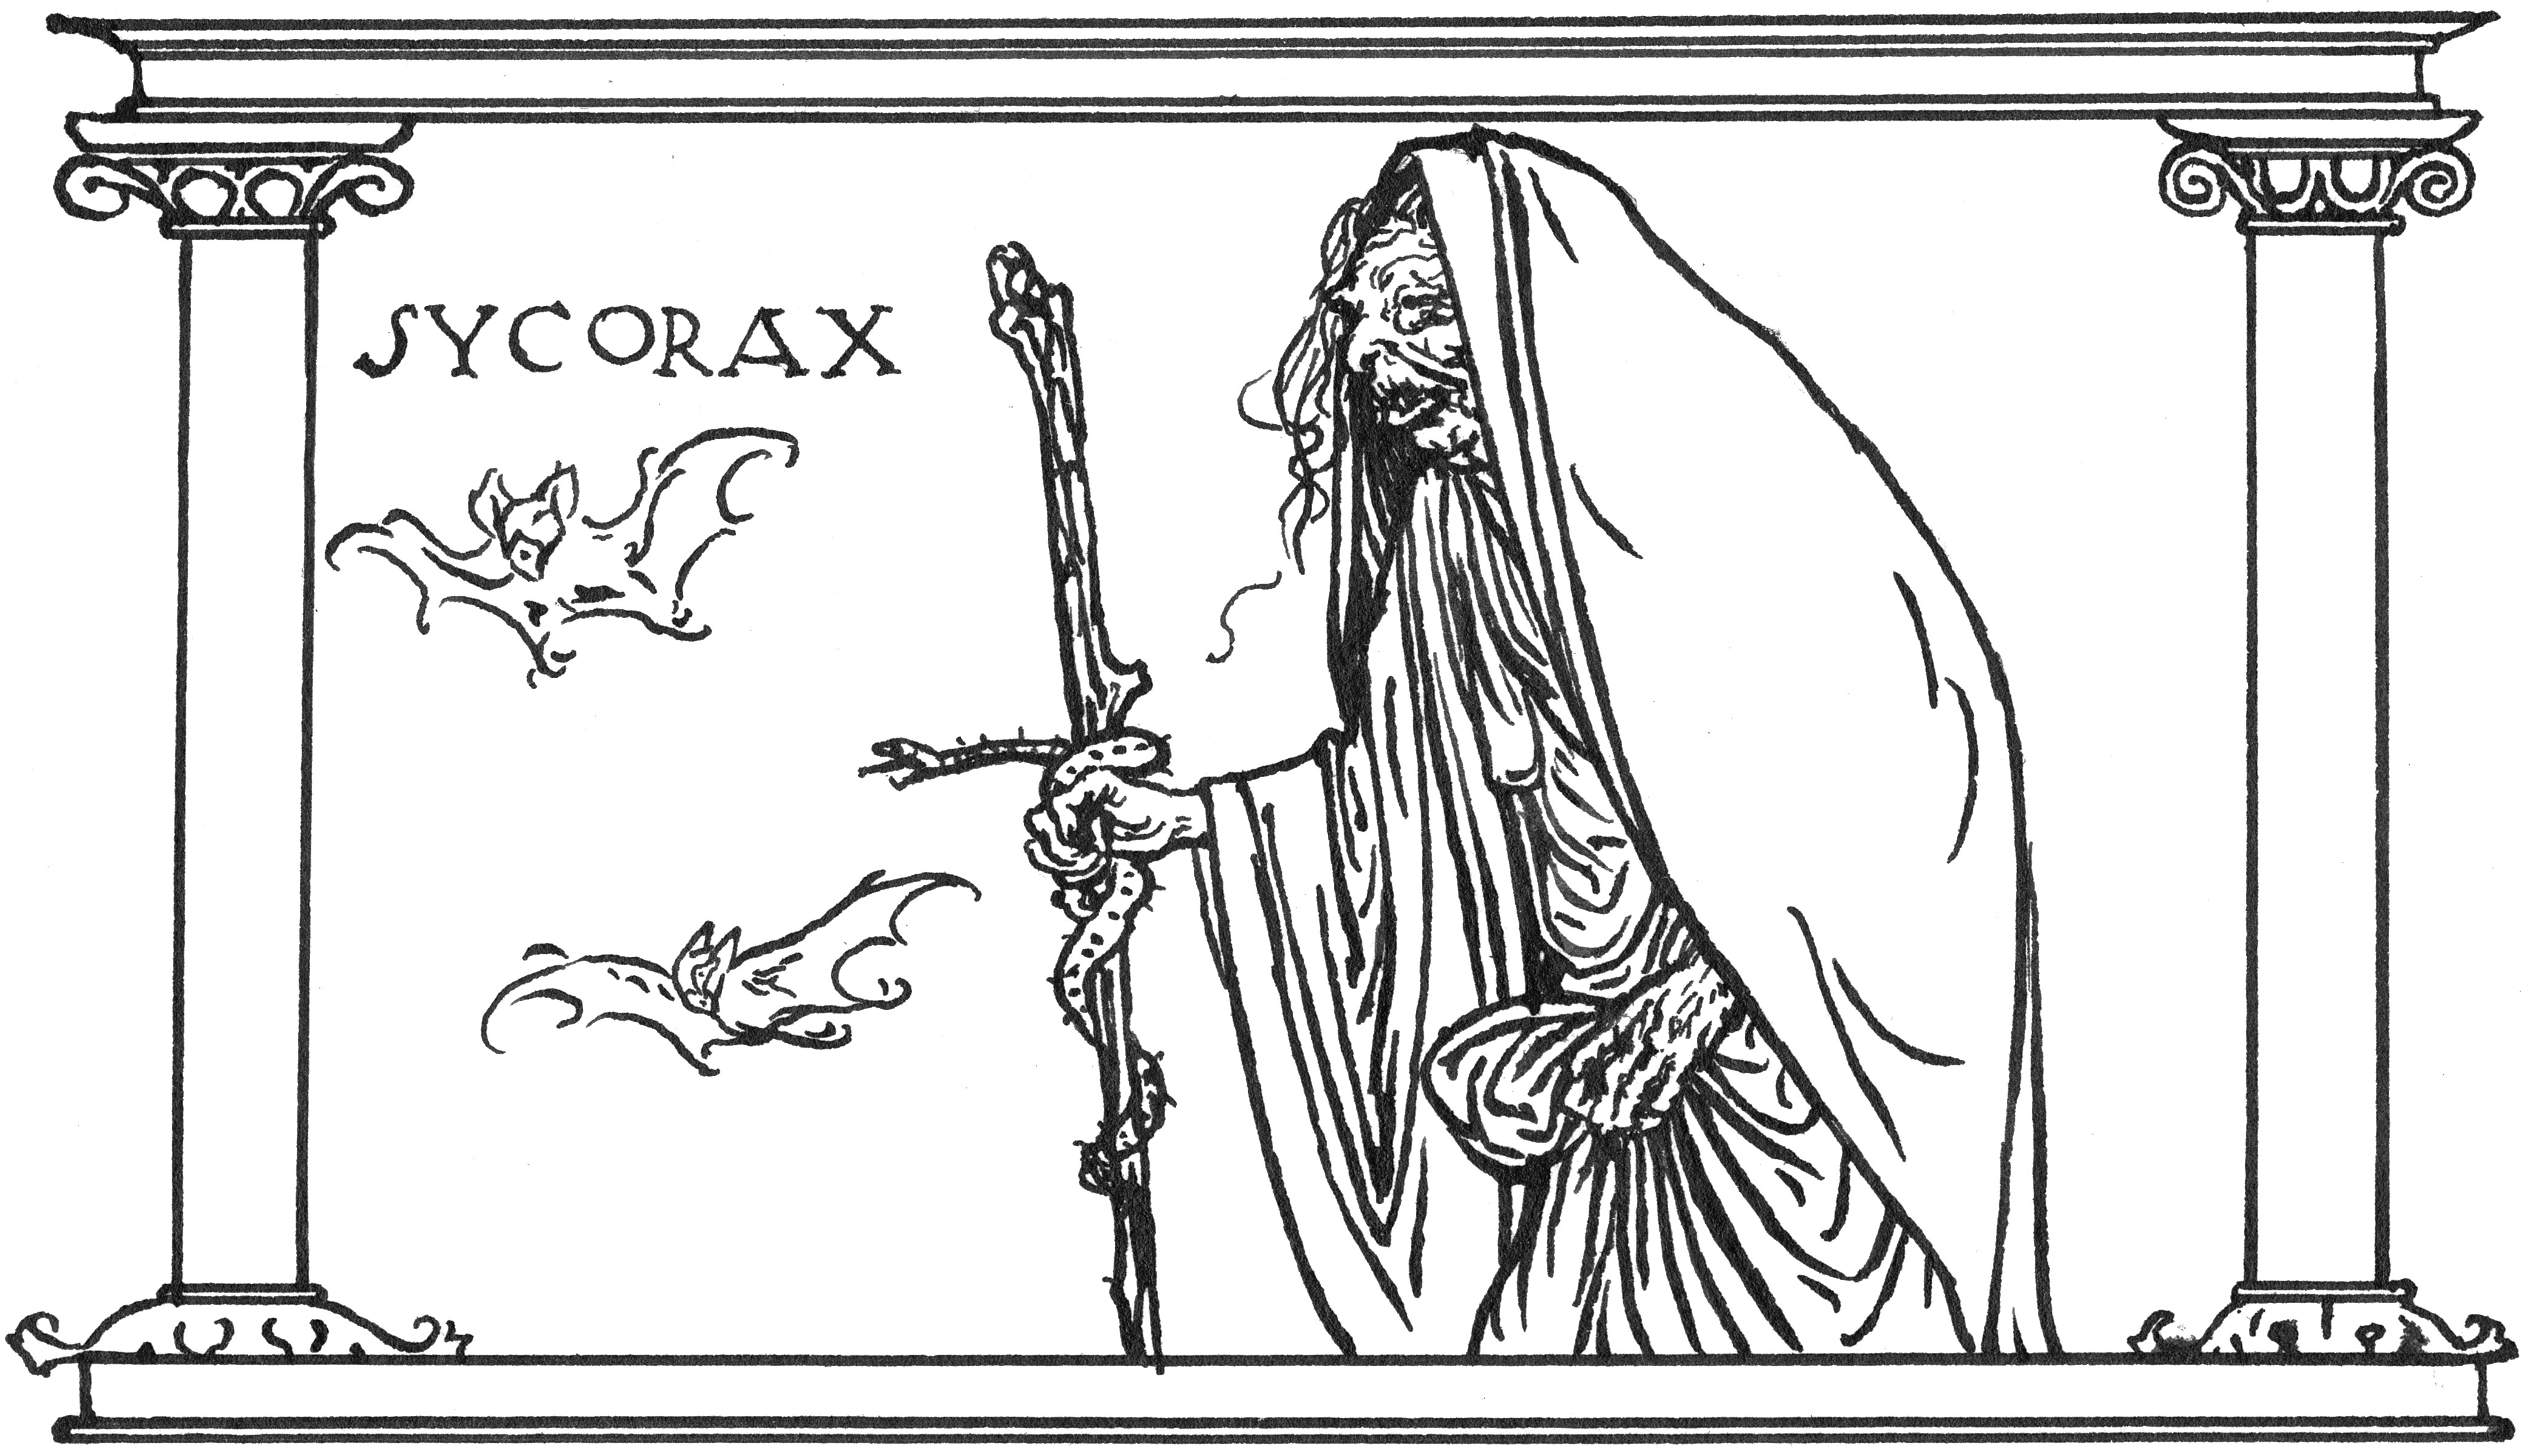
\includegraphics[width=0.8\textwidth]{1iisycorax}
\end{figure}

\begin{verse_speech}[Prospero] 
\hspace{\widthof{The rest o' the island.}}Thou most lying slave,\\
Whom stripes may move, not kindness! I have used thee,\\
Filth as thou art, with human care, and lodged thee\\
In mine own cell, till thou didst seek to violate\\
The honour of my child.
\end{verse_speech}

\begin{verse_speech}[Caliban]
O ho, O ho! would't had been done!\\
Thou didst prevent me; I had peopled else\\
This isle with Calibans.
\end{verse_speech}

\begin{verse_speech}[Miranda] 
\hspace{\widthof{This isle with Calibans.}}Abhorrèd slave,\\
Which any print of goodness wilt not take,\\
Being capable of all ill! I pitied thee,\\
Took pains to make thee speak, taught thee each hour\\
One thing or other: when thou didst not, savage,\\
Know thine own meaning, but wouldst gabble like\\
A thing most brutish, I endow'd thy purposes\\
With words that made them known. But thy vile race,\\
Though thou didst learn, had that in't which good natures\\
Could not abide to be with; therefore wast thou\\
Deservedly confined into this rock,\\
Who hadst deserved more than a prison.
\end{verse_speech}

\begin{verse_speech}[Caliban] 
You taught me language; and my profit on't\\
Is, I know how to curse. The red plague rid you\\
For learning me your language!
\end{verse_speech}

\begin{verse_speech}[Prospero] 
\hspace{\widthof{For learning me your language!}}Hag-seed, hence!\\
Fetch us in fuel; and be quick, thou'rt best,\\
To answer other business. Shrug'st thou, malice?\\
If thou neglect'st or dost unwillingly\\
What I command, I'll rack thee with old cramps,\\
Fill all thy bones with aches, make thee roar\\
That beasts shall tremble at thy din.
\end{verse_speech}

\begin{verse_speech}[Caliban] 
\hspace{\widthof{That beasts shall tremble at thy din.}}No, pray thee.\\
\aside{I must obey: his art is of such power,\\
It would control my dam's god, Setebos,\\
And make a vassal of him.}
\end{verse_speech}

\begin{verse_speech}[Prospero] 
\hspace{\widthof{And make a vassal of him.}}So, slave; hence!
\end{verse_speech}

\exit{\textsc{Caliban}}

\stage{Re-enter \textsc{Ariel}, invisible, playing and singing; \textsc{Ferdinand} following}

\begin{letter}
\begin{figure}[tbh]
	\centering
	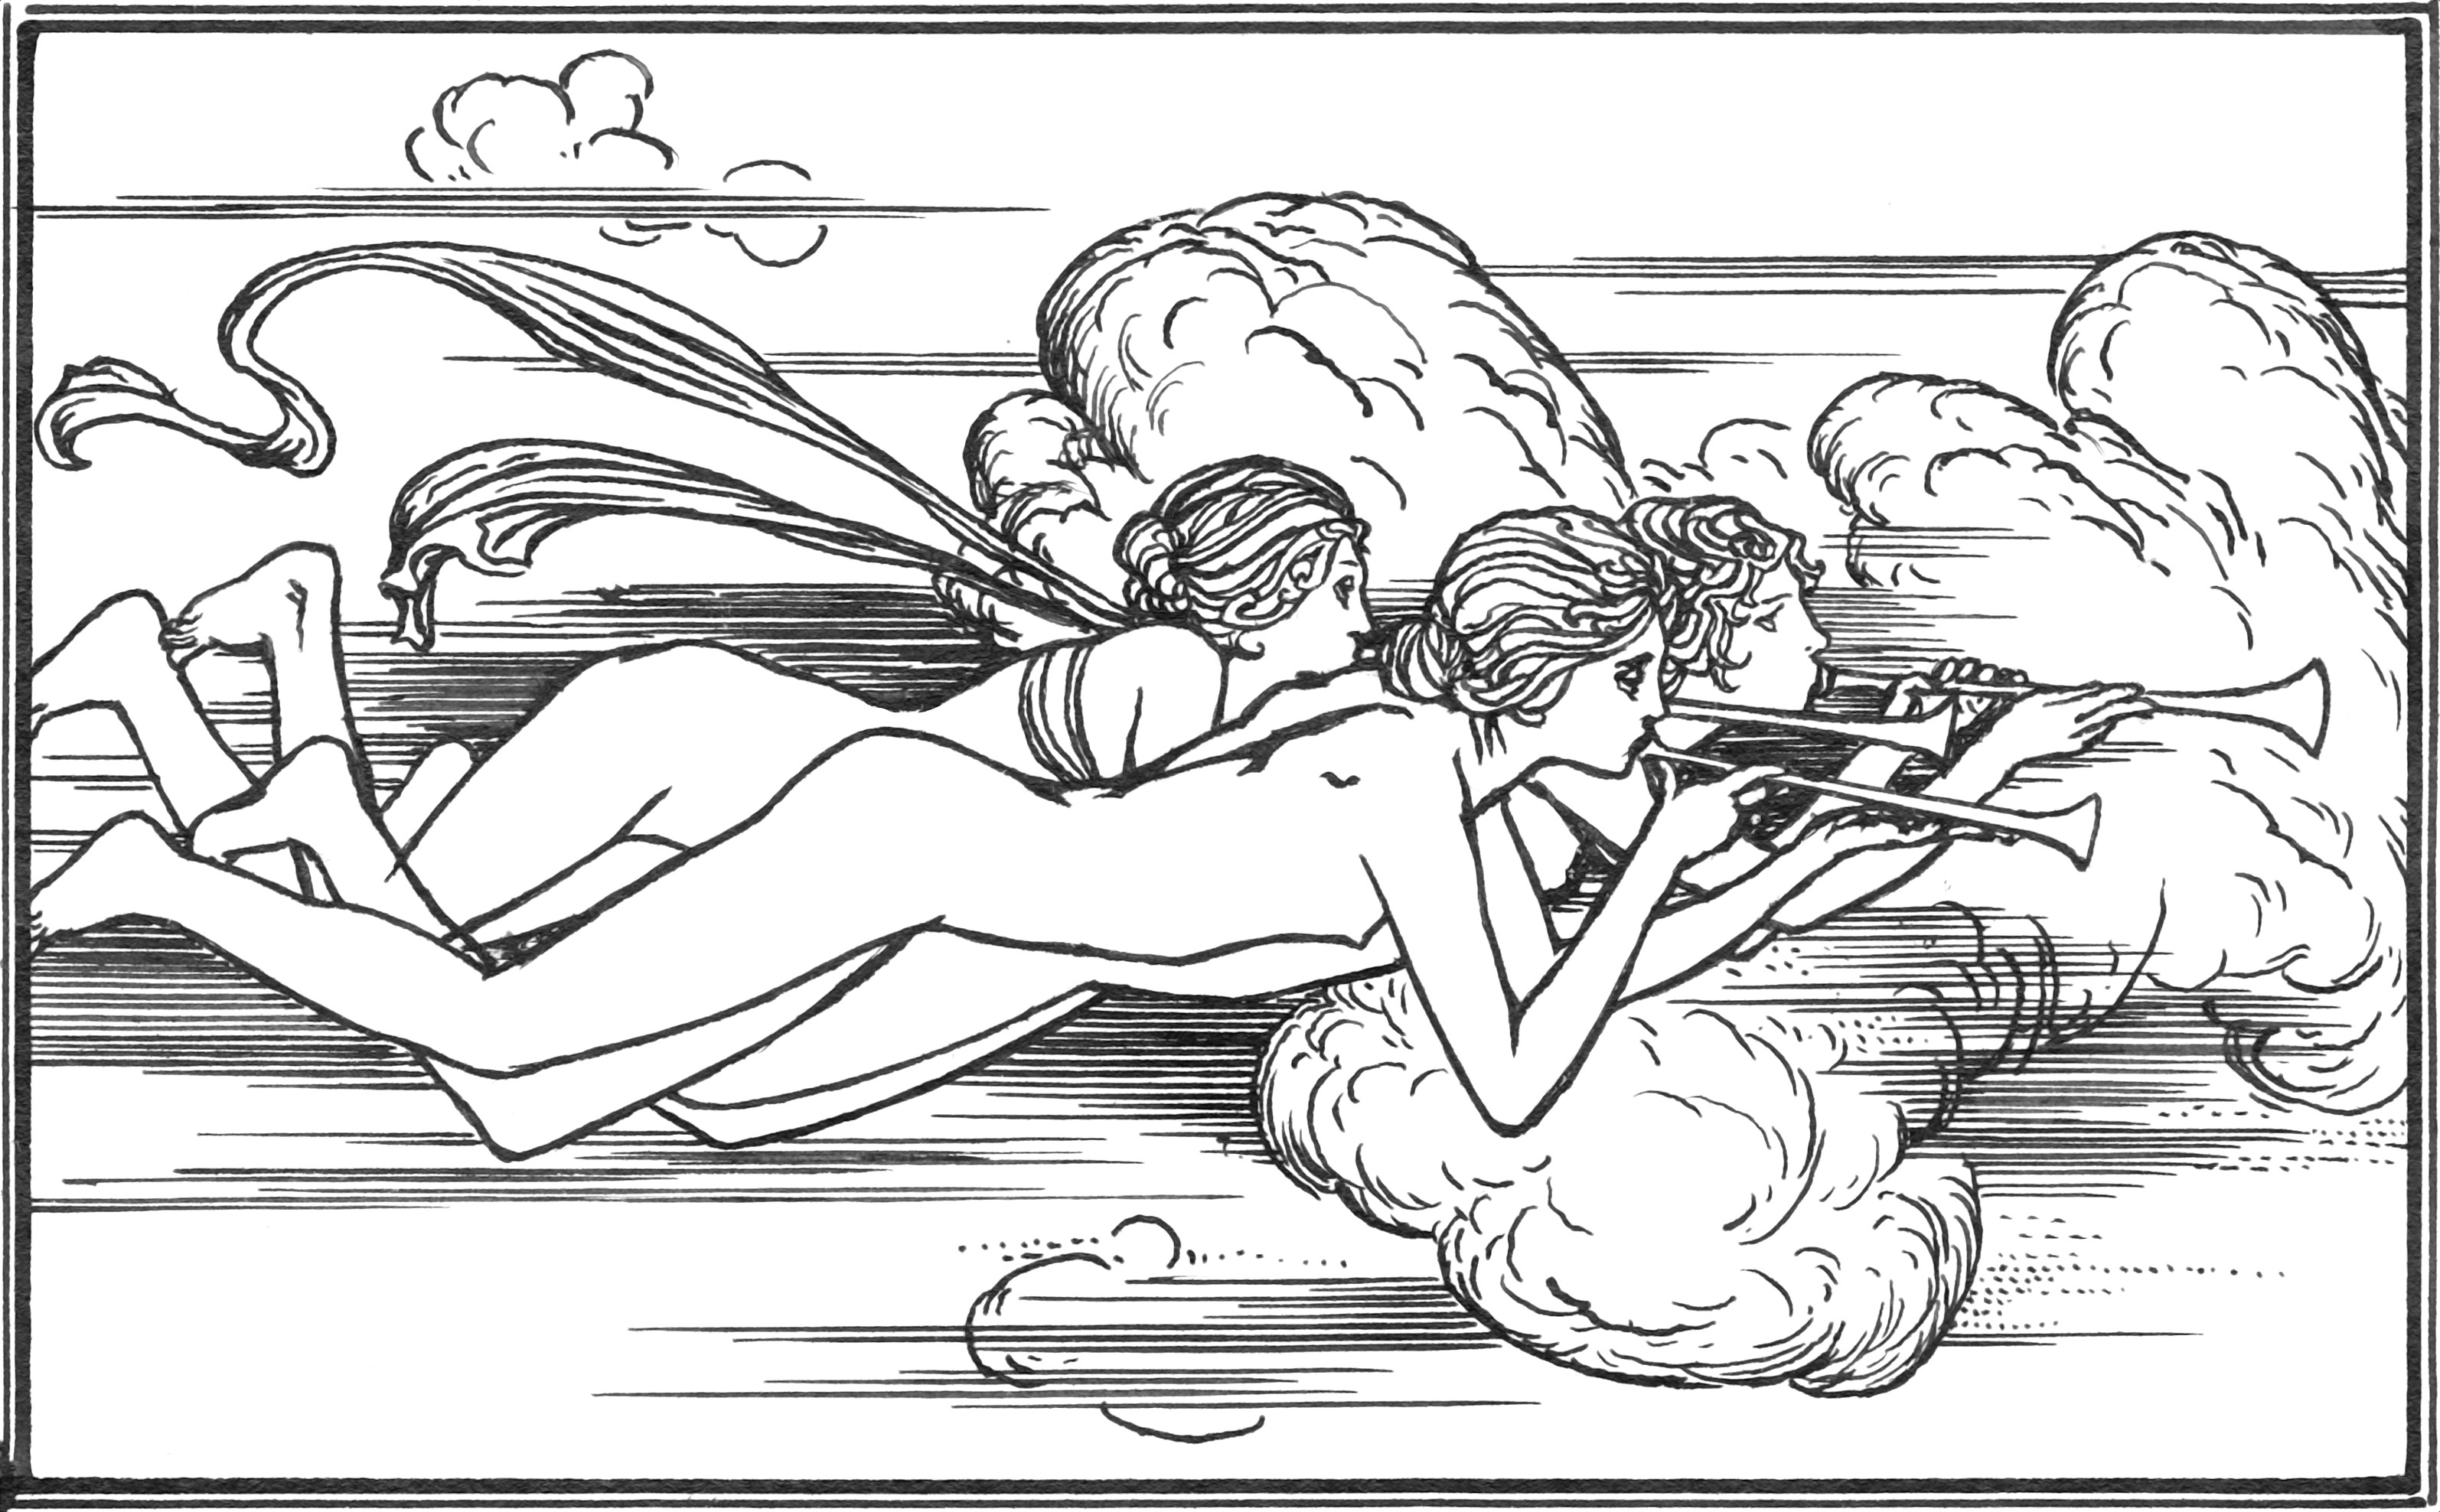
\includegraphics[width=0.8\textwidth]{1iitrumpets}
\end{figure}
\end{letter}

\begin{a4}
\vfill

\centerline{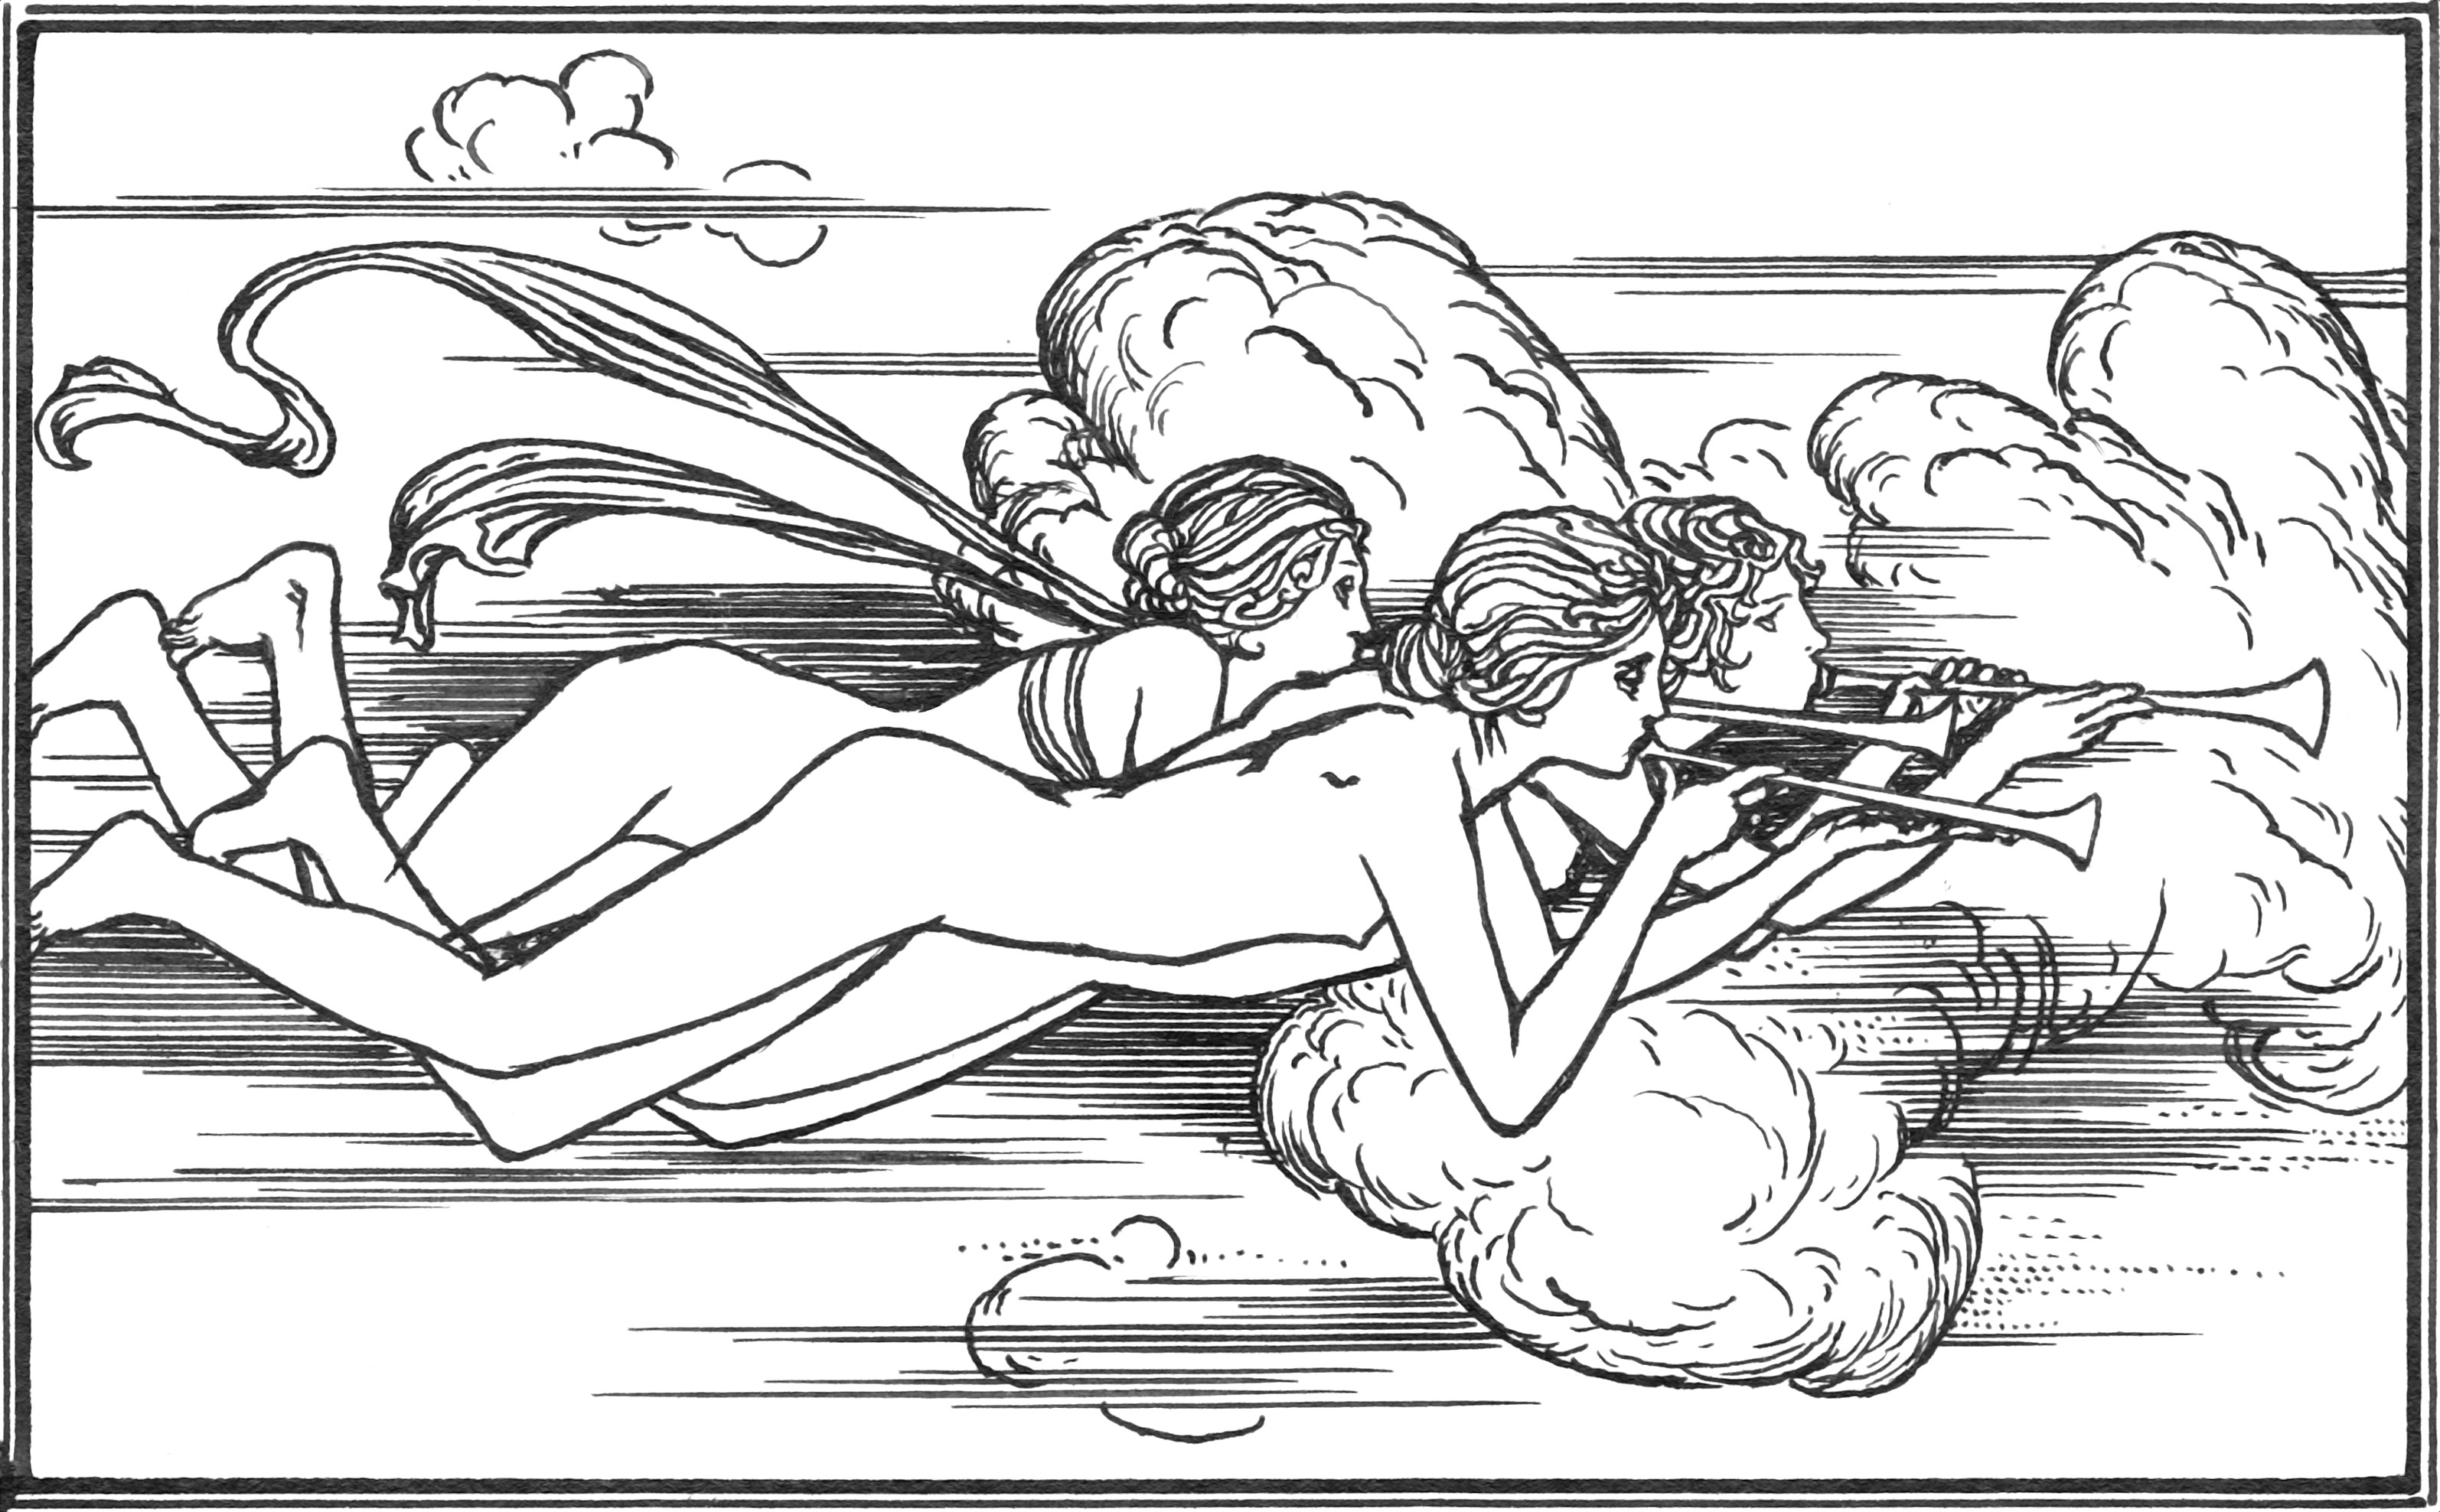
\includegraphics[width=\headerwidth]{1iitrumpets}}
\end{a4}

\begin{placeholder} %Ariel's song
	\clearpage
	\begin{song}[\textsc{Ariel's} song.]
		\songline{Come unto these yellow sands,}
		\songline{And then take hands:}
		\songline{Courtsied when you have and kiss'd}
		\songline{The wild waves whist,}
		\songline{Foot it featly here and there;}
		\songline{And, sweet sprites, the burthen bear.}
		\songline{Hark, hark!}
		\refrain{Bow-wow}
		\songline{The watch-dogs bark!}
		\refrain{Bow-wow}
		\songline{Hark, hark! I hear}
		\songline{The strain of strutting chanticleer}
		\songline{Cry, Cock-a-diddle-dow.}
	\end{song}
	\clearpage
\end{placeholder}

\begin{pictures} %Ariel's song
	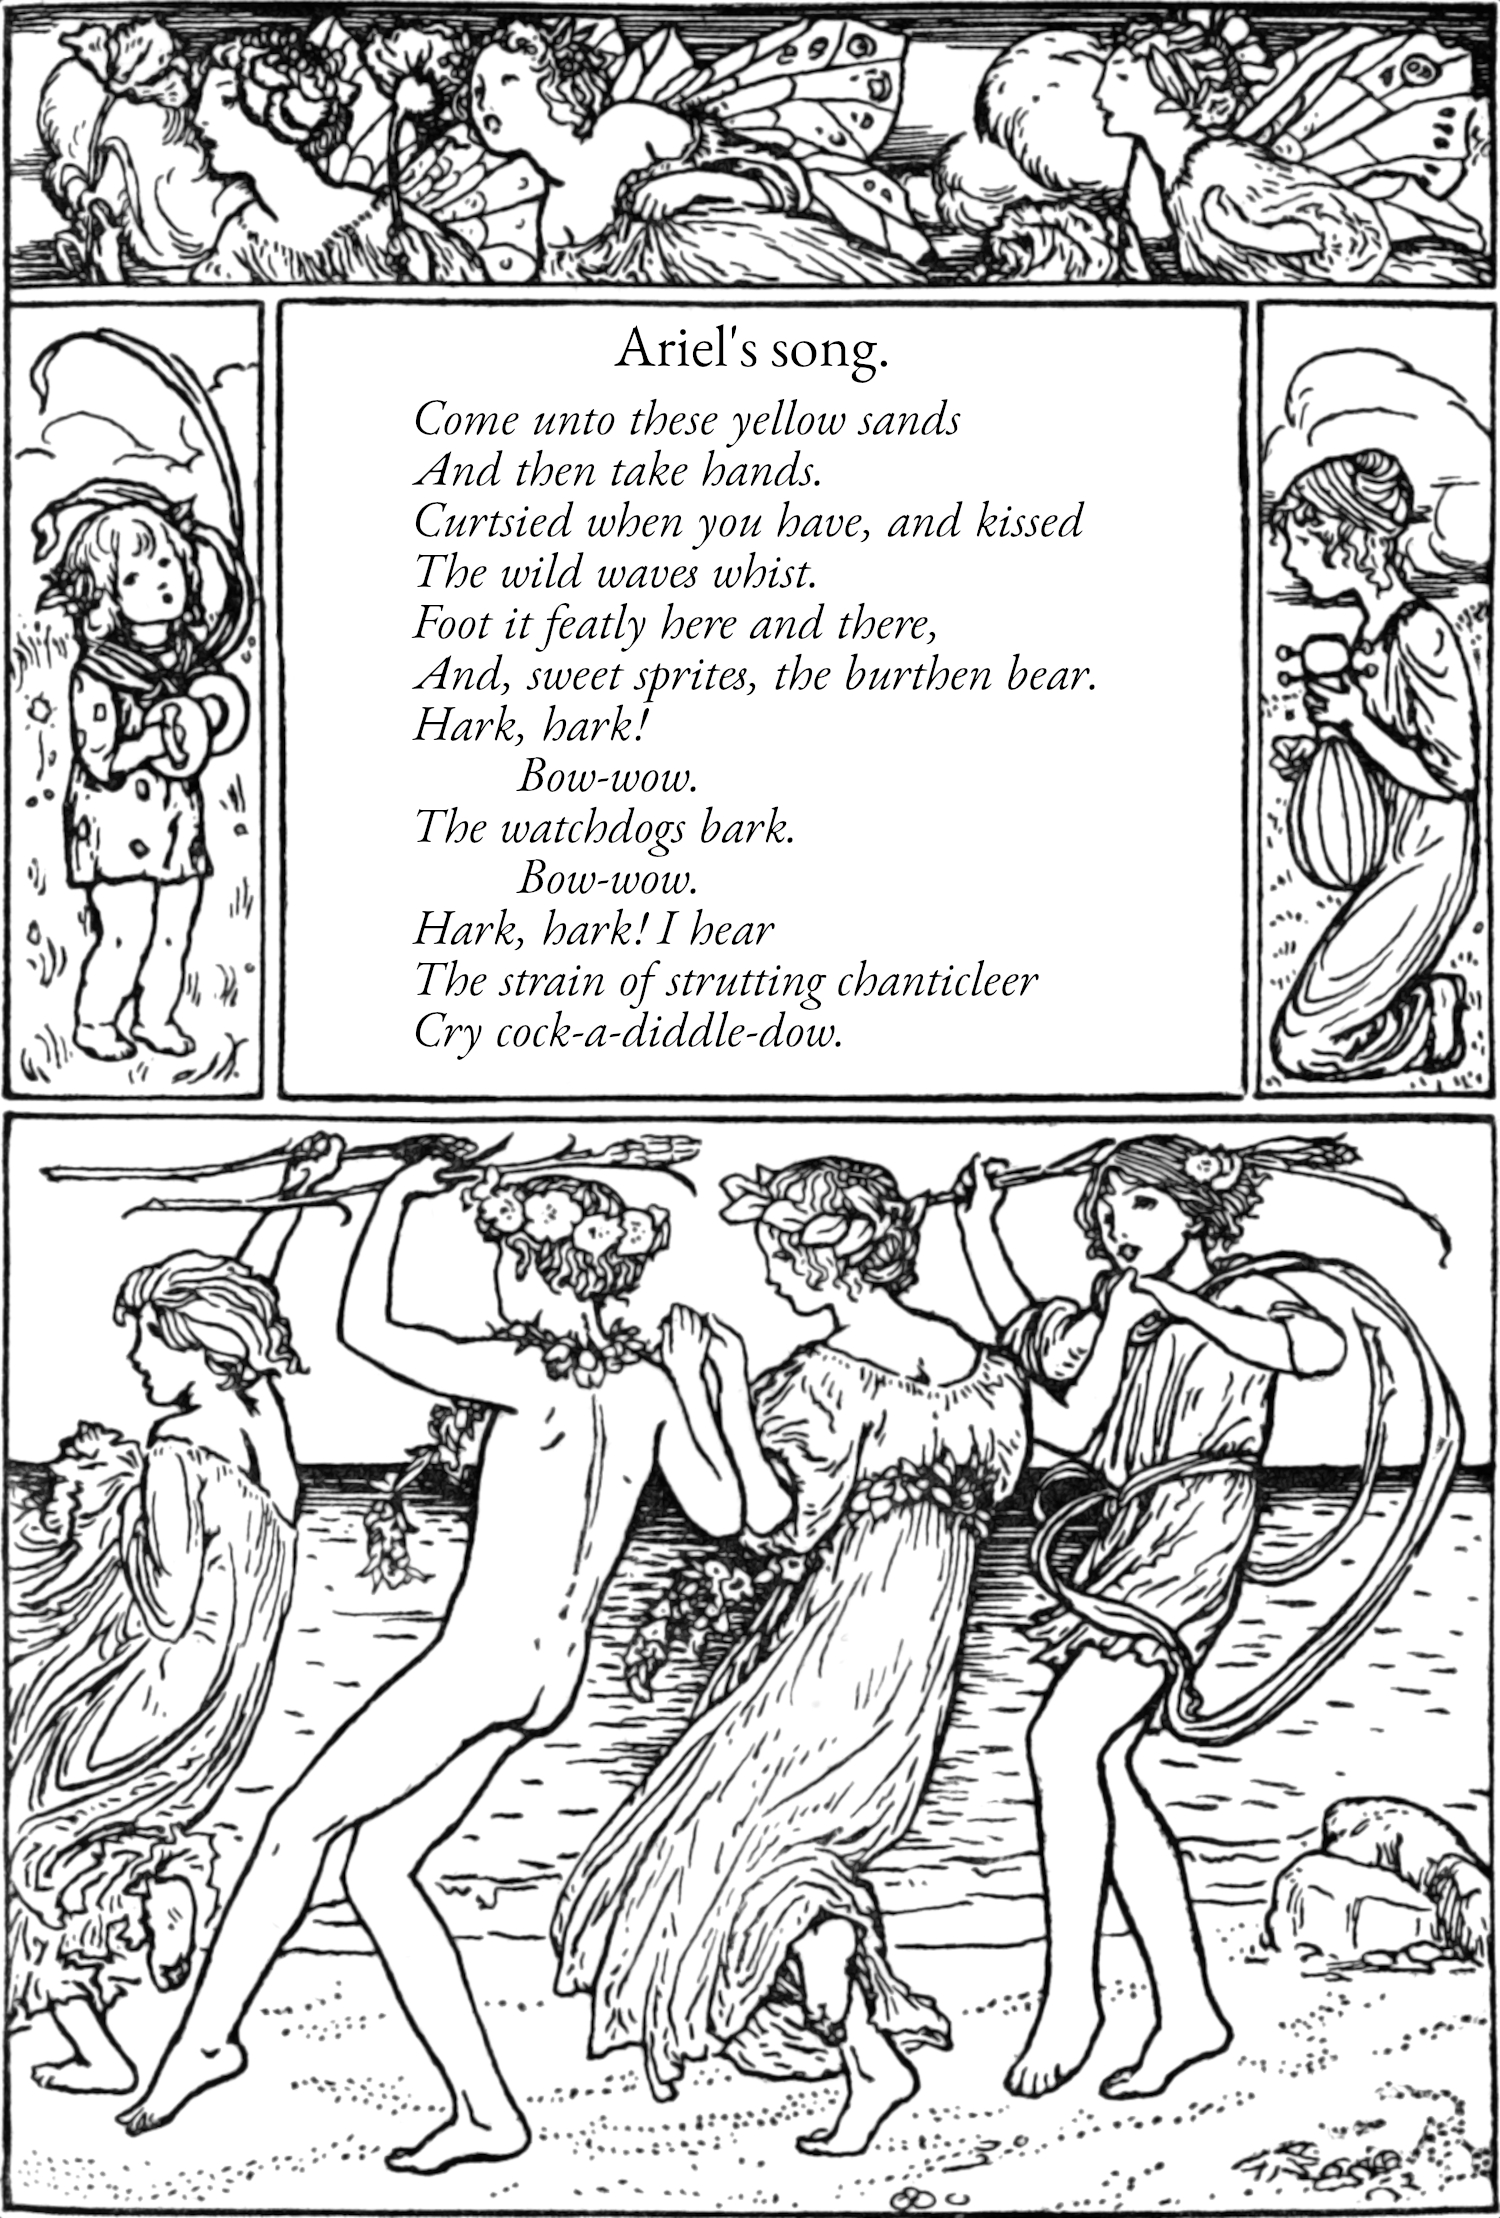
\includepdf[width=1.1\textwidth]{images/1iiarielsong.jpg}
\end{pictures}

%these can go anywhere between here and the float barrier


\begin{figure}[tbh]
\centering
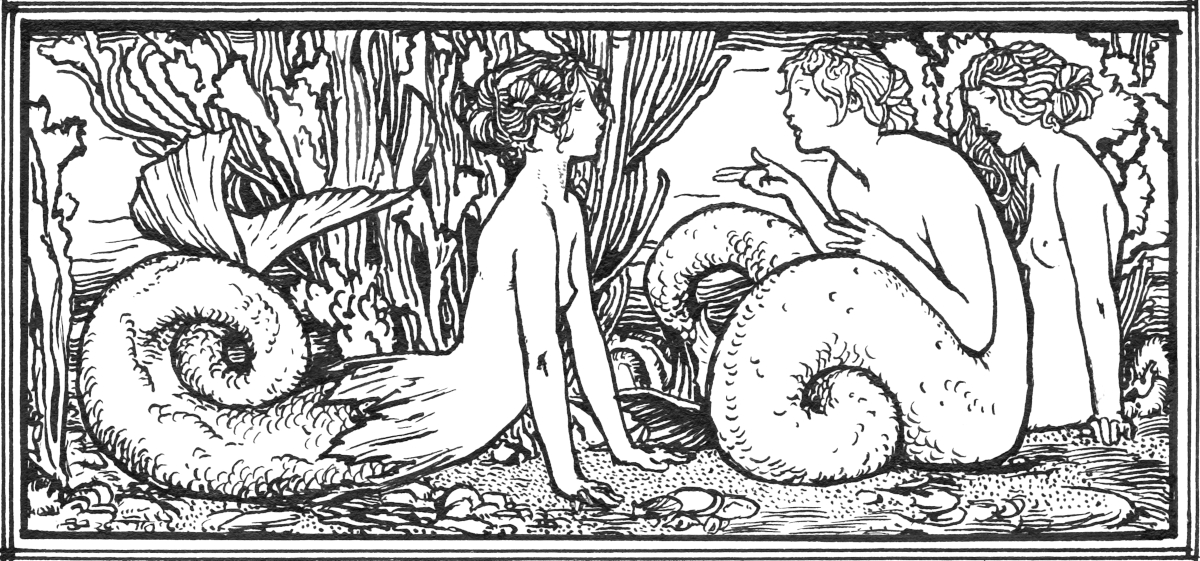
\includegraphics[width=\headerwidth]{1iimerconference}
\end{figure}

%end random decorations


\begin{pictures} %Full Fathom Five full page - a4
	\begin{a4}
		\begin{bwbigpic}
		[\picwidth]
		{1iifullfathomfive}
		{}
		\end{bwbigpic}
	\end{a4}
\end{pictures}

\begin{verse_speech}[Ferdinand] 
Where should this music be? i' the air or the earth?\\
It sounds no more: and sure, it waits upon\\
Some god o' the island. Sitting on a bank,\\
Weeping again the king my father's wreck,\\
This music crept by me upon the waters,\\
Allaying both their fury and my passion\\
With its sweet air: thence I have follow'd it,\\
Or it hath drawn me rather. But 'tis gone.\\
No, it begins again.
\stage{\textsc{Ariel} sings}
\begin{song}
\songline{Full fathom five thy father lies;}
\songline{Of his bones are coral made;}
\songline{Those are pearls that were his eyes:}
\songline{Nothing of him that doth fade}
\songline{But doth suffer a sea-change}
\songline{Into something rich and strange.}
\songline{Sea-nymphs hourly ring his knell}
\refrain{Ding-dong}
\songline{Hark! now I hear them,—}
\refrain{Ding-dong, bell.}
\end{song}
\end{verse_speech}




\begin{pictures} %Full Fathom Five full page - letter
	\begin{letter}
		\begin{bwbigpic}
		[\picwidth]
		{1iifullfathomfive}
		{}
		\end{bwbigpic}
	\end{letter}
\end{pictures}



\begin{verse_speech}[Ferdinand] 
The ditty does remember my drown'd father.\\
This is no mortal business, nor no sound\\
That the earth owes. I hear it now above me.\\
\end{verse_speech}



\begin{verse_speech}[Prospero] 
The fringèd curtains of thine eye advance\\
And say what thou seest yond.
\end{verse_speech}

\begin{verse_speech}[Miranda] 
\hspace{\widthof{And say what thou seest yond.}}What is't? a spirit?\\
Lord, how it looks about! Believe me, sir,\\
It carries a brave form. But 'tis a spirit.
\end{verse_speech}



\begin{verse_speech}[Prospero] 
No, wench; it eats and sleeps and hath such senses\\
As we have, such. This gallant which thou seest\\
Was in the wreck; and, but he's something stain'd\\
With grief that's beauty's canker, thou mightst call him\\
A goodly person: he hath lost his fellows\\
And strays about to find 'em.
\end{verse_speech}

\begin{verse_speech}[Miranda] 
\hspace{\widthof{And strays about to find 'em.}}I might call him\\
A thing divine, for nothing natural\\
I ever saw so noble.
\end{verse_speech}

\begin{verse_speech}[Prospero]\aside{\hspace{\widthof{I ever saw so noble.}-\widthof{[Aside]}}It goes on, I see,\\
As my soul prompts it. Spirit, fine spirit! I'll free thee\\
Within two days for this.}
\end{verse_speech}


\begin{pictures} %Ariel leads Ferdinand
	\begin{bwbigpic}
		[\picwidth]
		{1iiarielferdinand}
		{}
	\end{bwbigpic}
\end{pictures}



\begin{verse_speech}[Ferdinand] 
\hspace{\widthof{Within two days for this.}}Most sure, the goddess\\
On whom these airs attend! Vouchsafe my prayer\\
May know if you remain upon this island;\\
And that you will some good instruction give\\
How I may bear me here: my prime request,\\
Which I do last pronounce, is, O you wonder!\\
If you be maid or no?
\end{verse_speech}

\begin{verse_speech}[Miranda] 
\hspace{\widthof{If you be maid or no?}}No wonder, sir;\\
But certainly a maid.
\end{verse_speech}

\begin{verse_speech}[Ferdinand] 
\hspace{\widthof{But certainly a maid.}}My language! heavens!\\
I am the best of them that speak this speech,\\
Were I but where 'tis spoken.
\end{verse_speech}

\begin{verse_speech}[Prospero] 
\hspace{\widthof{Were I but where 'tis spoken.}}How? the best?\\
What wert thou, if the King of Naples heard thee?
\end{verse_speech}

\begin{verse_speech}[Ferdinand] 
A single thing, as I am now, that wonders\\
To hear thee speak of Naples. He does hear me;\\
And that he does I weep: myself am Naples,\\
Who with mine eyes, never since at ebb, beheld\\
The king my father wreck'd.
\end{verse_speech}

\verseline[Miranda]{\hspace{\widthof{The king my father wreck'd.}}Alack, for mercy!}
	
\begin{verse_speech}[Ferdinand] 
Yes, faith, and all his lords; the Duke of Milan\\
And his brave son being twain.
\end{verse_speech}


\begin{pictures} %Ferdinand meets Miranda
	\begin{bwbigpic}
		[\picwidth]
		{1iiferdmiranda}
		{}
	\end{bwbigpic}
\end{pictures}



\begin{verse_speech}[Prospero] \aside{\hspace{\widthof{And his brave son being twain.}-\widthof{[Aside]}}The Duke of Milan\\
And his more braver daughter could control thee,\\
If now 'twere fit to do't. At the first sight\\
They have changed eyes. Delicate Ariel,\\
I'll set thee free for this.}
\stage{To \textsc{Ferdinand}}
\hspace{\widthof{I'll set thee free for this.}}A word, good sir;\\
I fear you have done yourself some wrong: a word.
\end{verse_speech}

\begin{verse_speech}[Miranda] 
Why speaks my father so ungently? This\\
Is the third man that e'er I saw, the first\\
That e'er I sigh'd for: pity move my father\\
To be inclined my way!
\end{verse_speech}

\begin{verse_speech}[Ferdinand] 
\hspace{\widthof{To be inclined my way!}}O, if a virgin,\\
And your affection not gone forth, I'll make you\\
The queen of Naples.
\end{verse_speech}

\begin{figure}[tb]
\centering
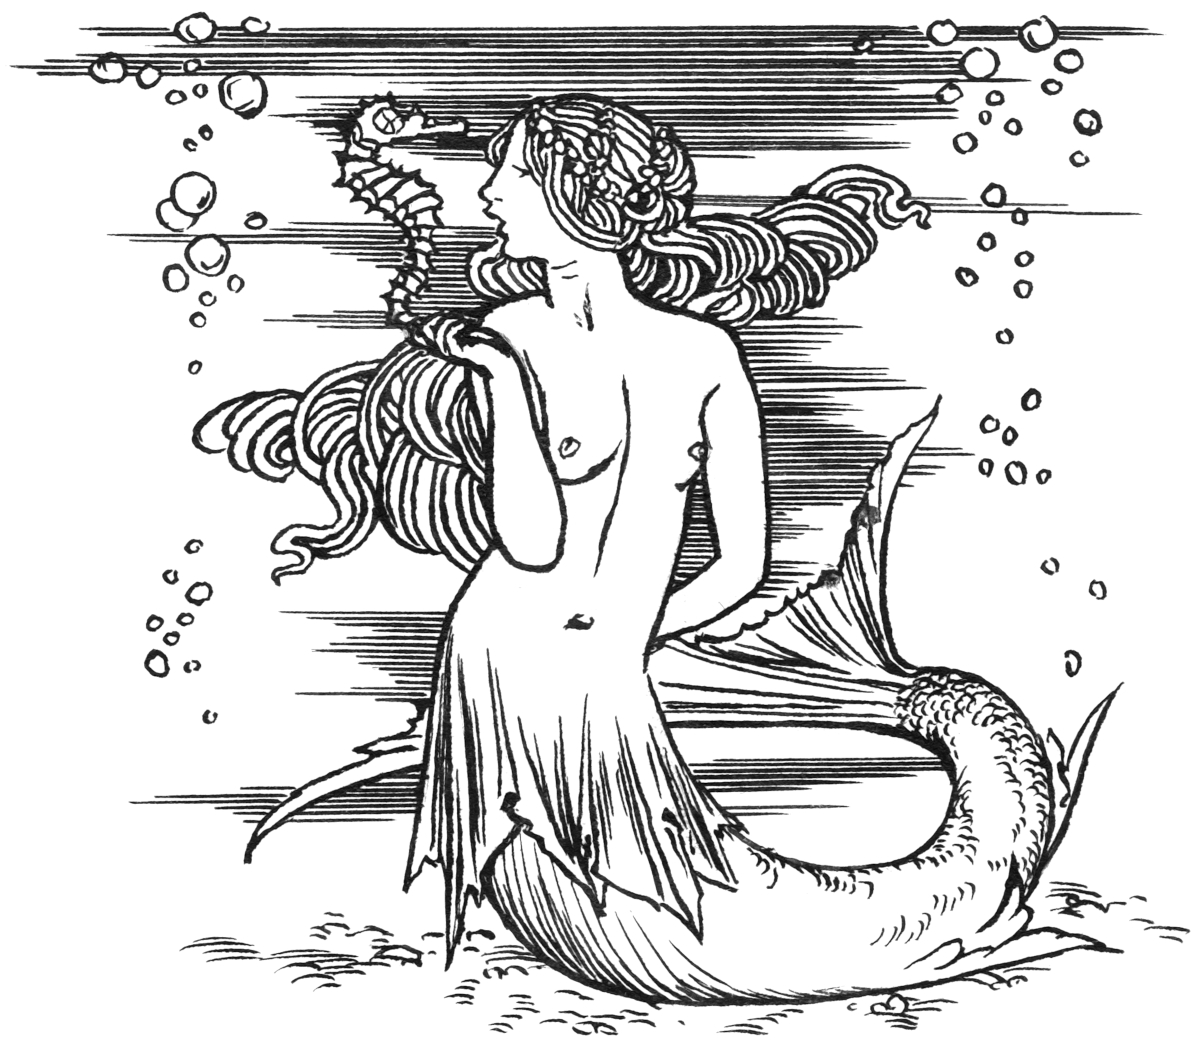
\includegraphics[width=\smallwidth]{1iimerseahorse}
\end{figure}

\begin{verse_speech}[Prospero] 
\hspace{\widthof{The queen of Naples.}}Soft, sir! one word more.\\
\aside{They are both in either's powers; but this swift business\\
I must uneasy make, lest too light winning\\
Make the prize light.}
\stage{To \textsc{Ferdinand}}
\hspace{\widthof{Make the prize light.}}One word more; I charge thee\\
That thou attend me: thou dost here usurp\\
The name thou owest not; and hast put thyself\\
Upon this island as a spy, to win it\\
From me, the lord on't.
\end{verse_speech}

\verseline[Ferdinand]{\hspace{\widthof{From me, the lord on't.}}No, as I am a man.}
	
\begin{verse_speech}[Miranda] 
There's nothing ill can dwell in such a temple:\\
If the ill spirit have so fair a house,\\
Good things will strive to dwell with't.
\end{verse_speech}

\begin{verse_speech}[Prospero] 
\stage{To \textsc{Ferdinand}}
\hspace{\widthof{Good things will strive to dwell with't.}}Follow me.\\
\stage{To \textsc{Miranda}}

Speak not you for him; he's a traitor. \\
\stage{To \textsc{Ferdinand}}

\begin{figure}[tb]
\centering
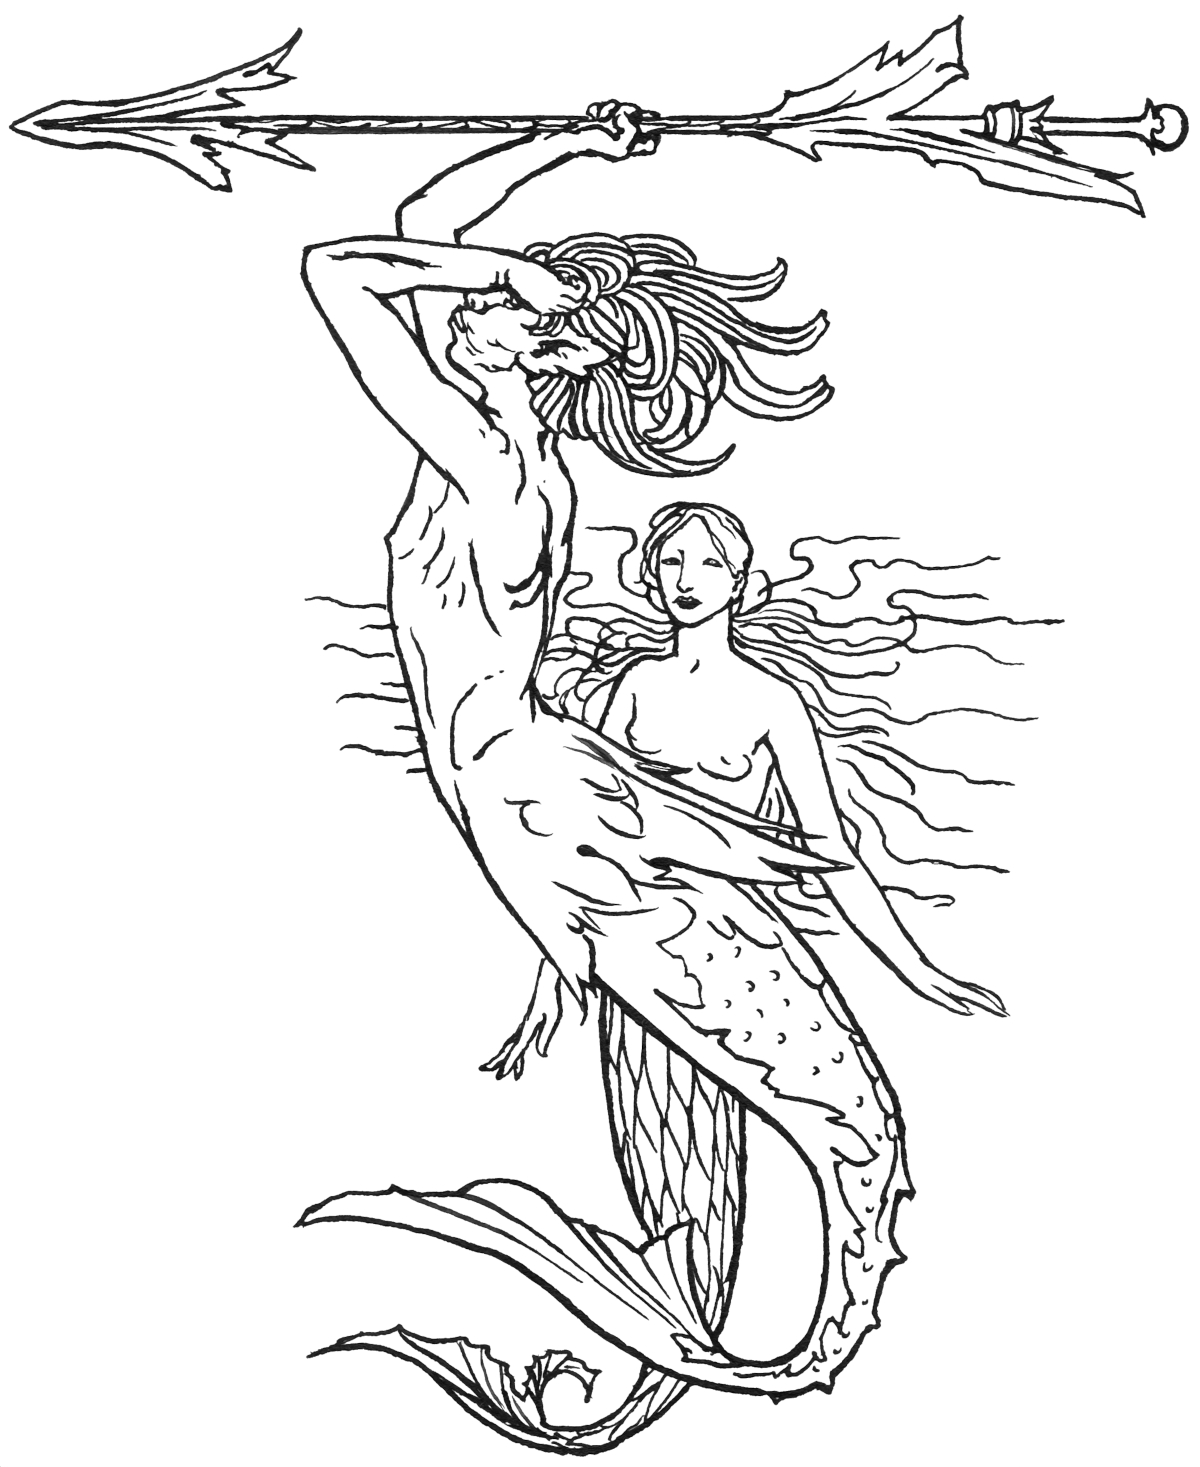
\includegraphics[width=.6\textwidth]{1iimerharpoon}
\end{figure}

\hspace{\widthof{Speak not you for him; he's a traitor.}}Come;\\
I'll manacle thy neck and feet together:\\
Sea-water shalt thou drink; thy food shall be\\
The fresh-brook muscles, wither'd roots and husks\\
Wherein the acorn cradled. Follow.\\
\end{verse_speech}

\begin{verse_speech}[Ferdinand] 
\hspace{\widthof{Wherein the acorn cradled. Follow.}}No;\\
I will resist such entertainment till\\
Mine enemy has more power.
\end{verse_speech}

\stage{He draws, and is charmed from moving}

\begin{verse_speech}[Miranda] 
\hspace{\widthof{Mine enemy has more power.}}O dear father,\\
Make not too rash a trial of him, for\\
He's gentle and not fearful.
\end{verse_speech}

\begin{verse_speech}[Prospero] 
\hspace{\widthof{He's gentle and not fearful.}}What? I say,\\
My foot my tutor? Put thy sword up, traitor;\\
Who makest a show but darest not strike, thy conscience\\
Is so possess'd with guilt: come from thy ward,\\
For I can here disarm thee with this stick\\
And make thy weapon drop.
\end{verse_speech}

\verseline[Miranda]{\hspace{\widthof{And make thy weapon drop.}}Beseech you, father.}
	
\verseline[Prospero]{Hence! hang not on my garments.}
	
\begin{verse_speech}[Miranda] 
\hspace{\widthof{Hence! hang not on my garments.}}Sir, have pity;\\
I'll be his surety.
\end{verse_speech}

\begin{verse_speech}[Prospero] 
\hspace{\widthof{I'll be his surety.}}Silence! one word more\\
Shall make me chide thee, if not hate thee. What!\\
An advocate for an imposter! hush!\\
Thou think'st there is no more such shapes as he,\\
Having seen but him and Caliban: foolish wench!\\
To the most of men this is a Caliban\\
And they to him are angels.
\end{verse_speech}

\begin{verse_speech}[Miranda] 
\hspace{\widthof{And they to him are angels.}}My affections\\
Are then most humble; I have no ambition\\
To see a goodlier man.
\end{verse_speech}

\begin{verse_speech}[Prospero] 
	\stage{To \textsc{Ferdinand}}
\hspace{\widthof{To see a goodlier man.}}Come on; obey:\\
Thy nerves are in their infancy again\\
And have no vigour in them.
\end{verse_speech}

\begin{verse_speech}[Ferdinand] 
\hspace{\widthof{And have no vigour in them.}}So they are;\\
My spirits, as in a dream, are all bound up.\\
My father's loss, the weakness which I feel,\\
The wreck of all my friends, nor this man's threats,\\
To whom I am subdued, are but light to me,\\
Might I but through my prison once a day\\
Behold this maid: all corners else o' the earth\\
Let liberty make use of; space enough\\
Have I in such a prison.
\end{verse_speech}

\begin{verse_speech}[Prospero] \aside{\hspace{\widthof{Have I in such a prison.}-\widthof{[Aside]}}It works.}
\stage{To \textsc{Ferdinand}}
\hspace{\widthof{Have I in such a prison. It works.}-\widthof{[Aside]}}Come on.\\
Thou hast done well, fine Ariel!
\stage{To \textsc{Ferdinand}}
Follow me.
\stage{To \textsc{Ariel}}
Hark what thou else shalt do me.
\end{verse_speech}

\begin{verse_speech}[Miranda] 
Be of comfort;\\
My father's of a better nature, sir,\\
Than he appears by speech: this is unwonted\\
Which now came from him.
\end{verse_speech}

\begin{verse_speech}[Prospero] 
Thou shalt be free\\
As mountain winds: but then exactly do\\
All points of my command.
\end{verse_speech}

\verseline[Ariel]{To the syllable.}

\verseline[Prospero]{Come, follow. Speak not for him.}
\exeunt{}


%tailpiece
\begin{letter}
	\vfill
	\centerline{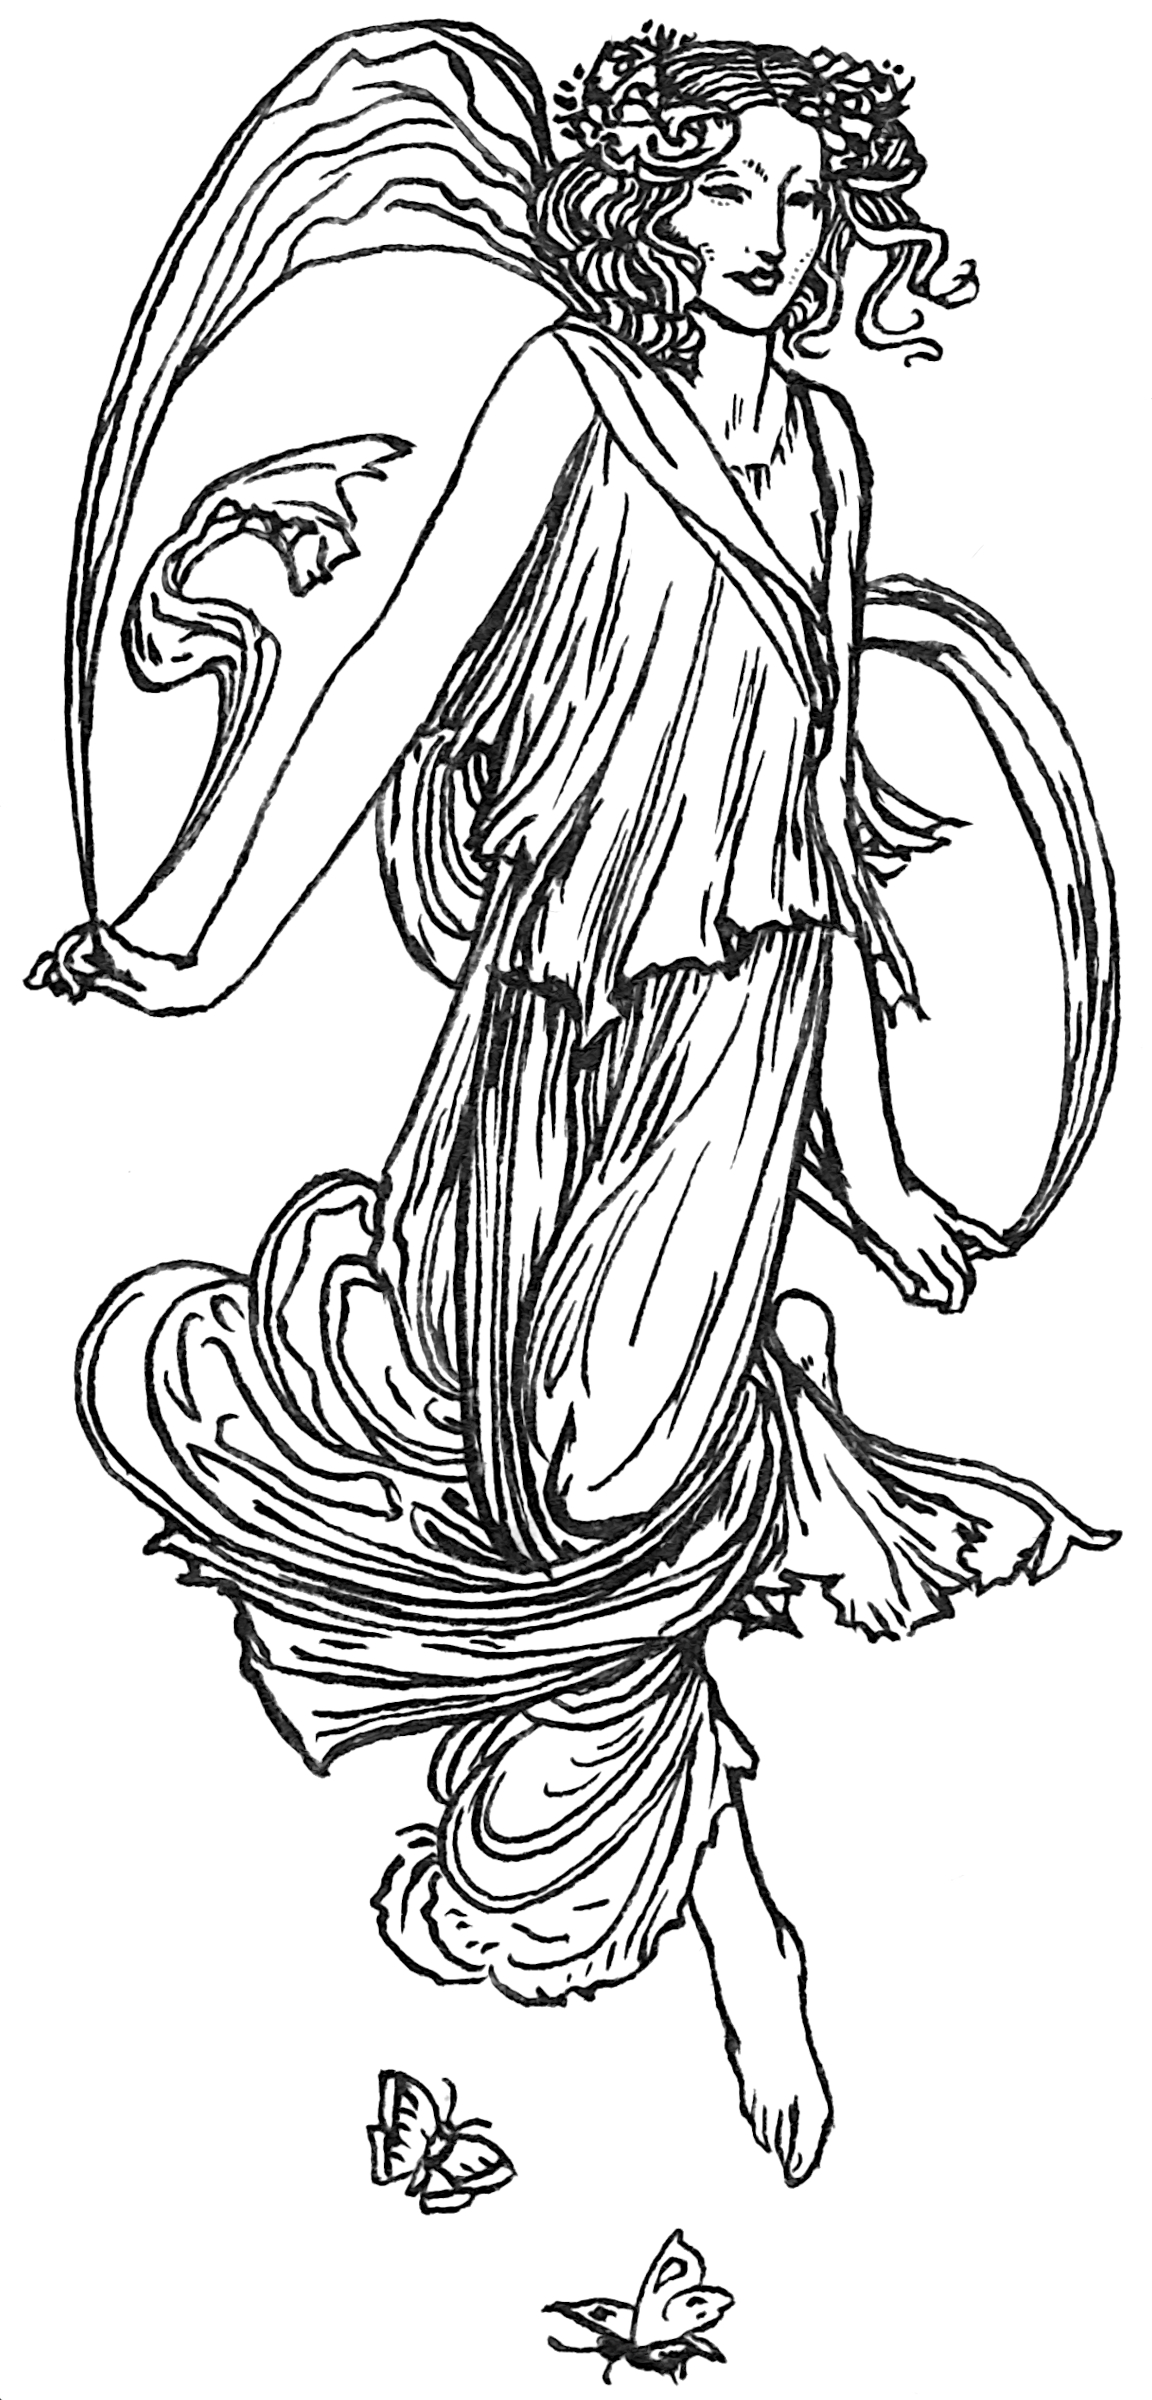
\includegraphics[width=.4\textwidth]{1iiarieltailpiece}}

\end{letter}
\begin{a4}
	\begin{tikzpicture}[remember picture, overlay]
		\node (dropcap) at ($(current page.south)+(0cm,6cm)$) {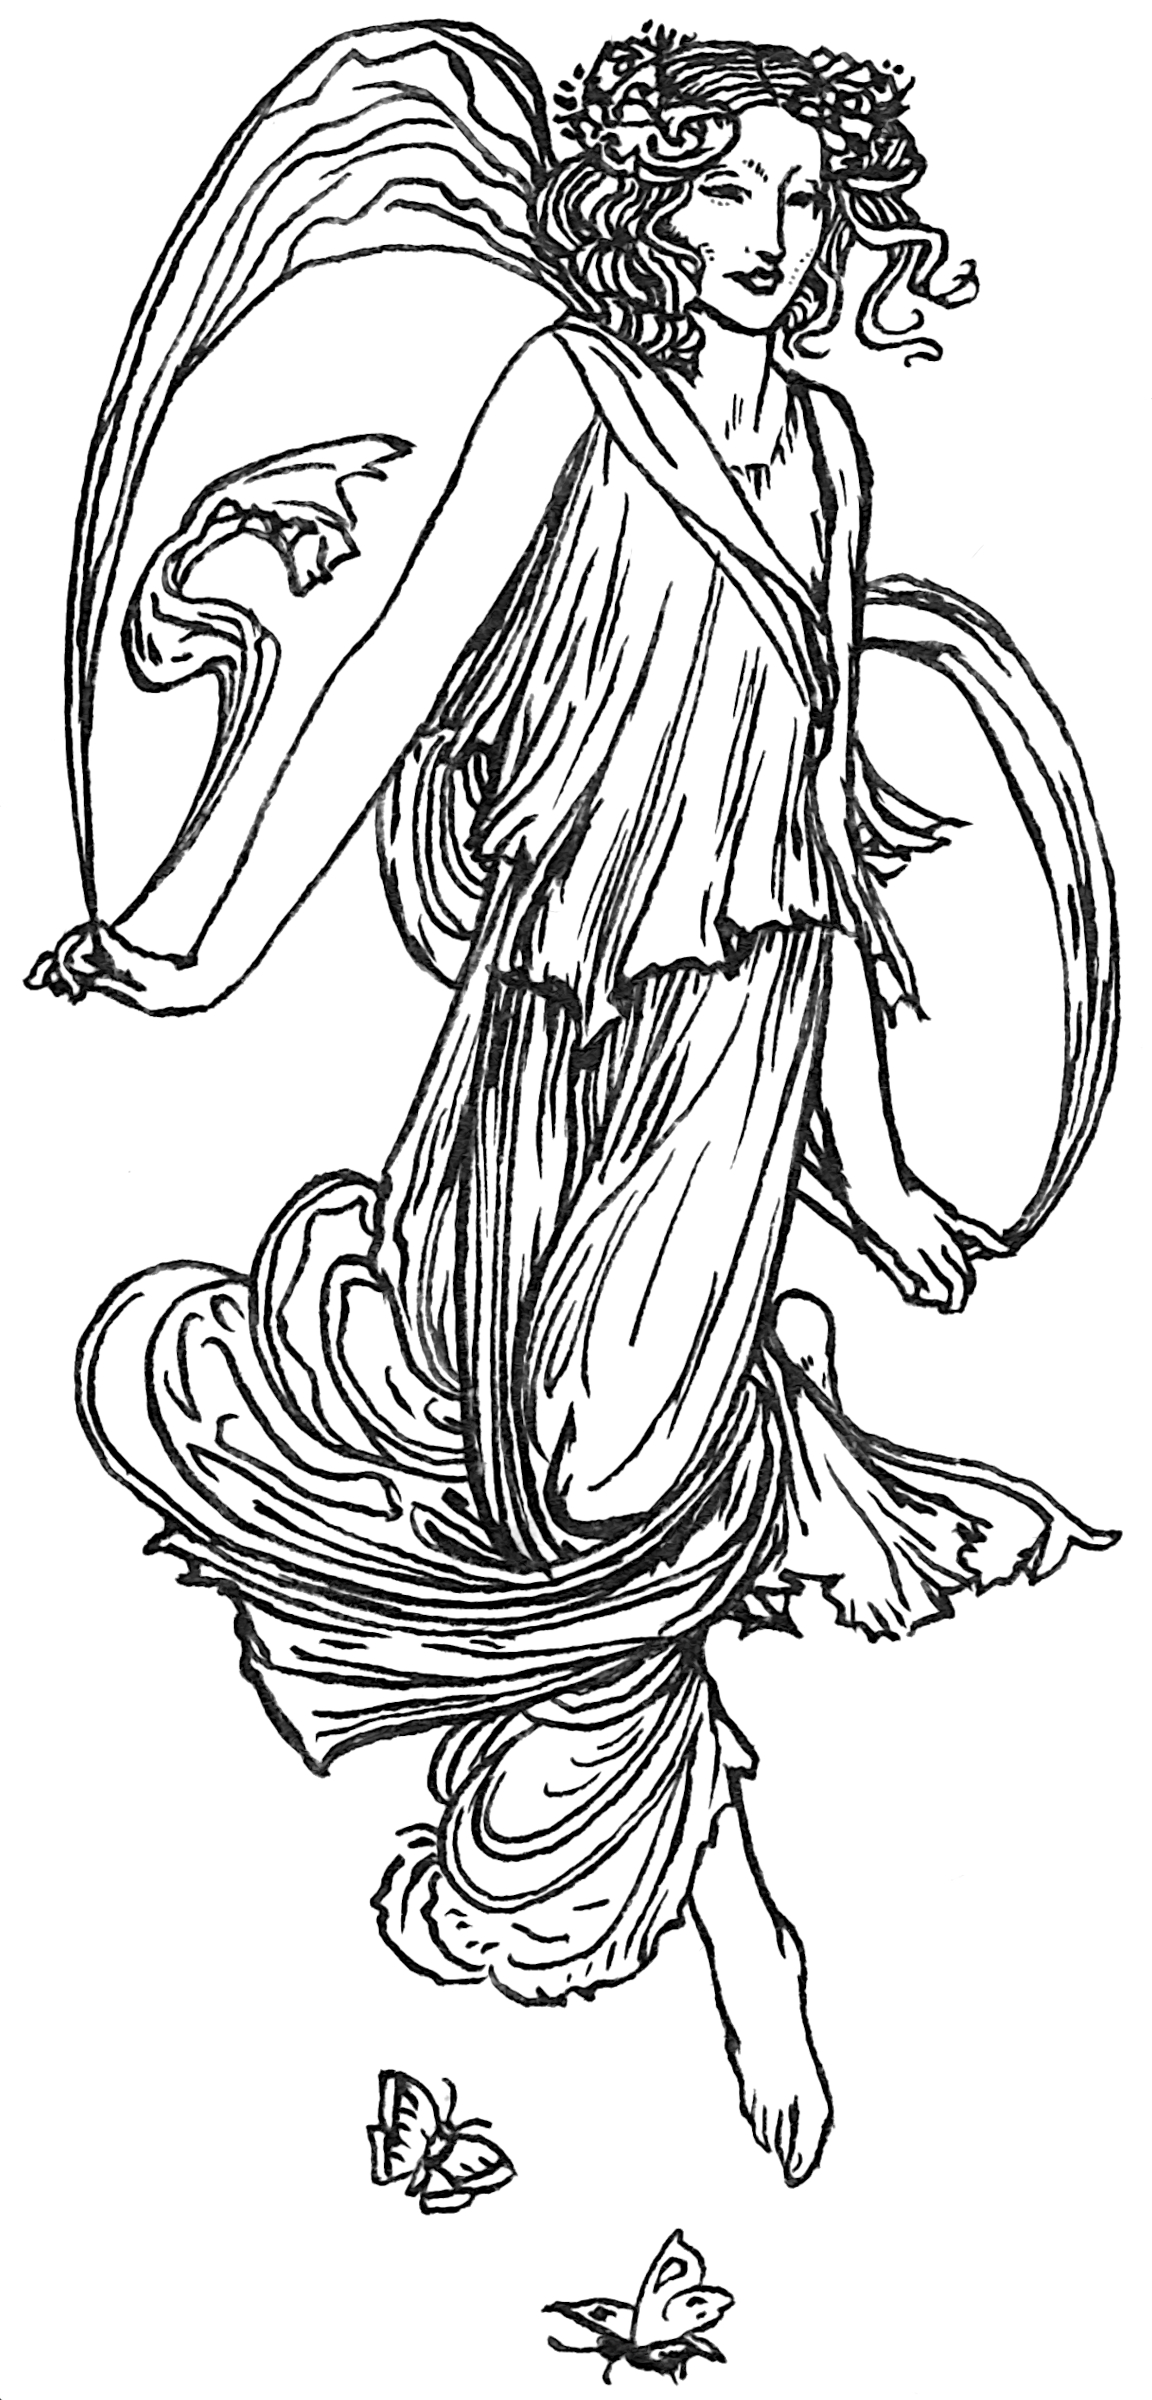
\includegraphics[width=.35\textwidth]{1iiarieltailpiece}};
	\end{tikzpicture}
\end{a4}

\begin{pictures}
	\cleardoubleevenpage
	\begin{letter}
		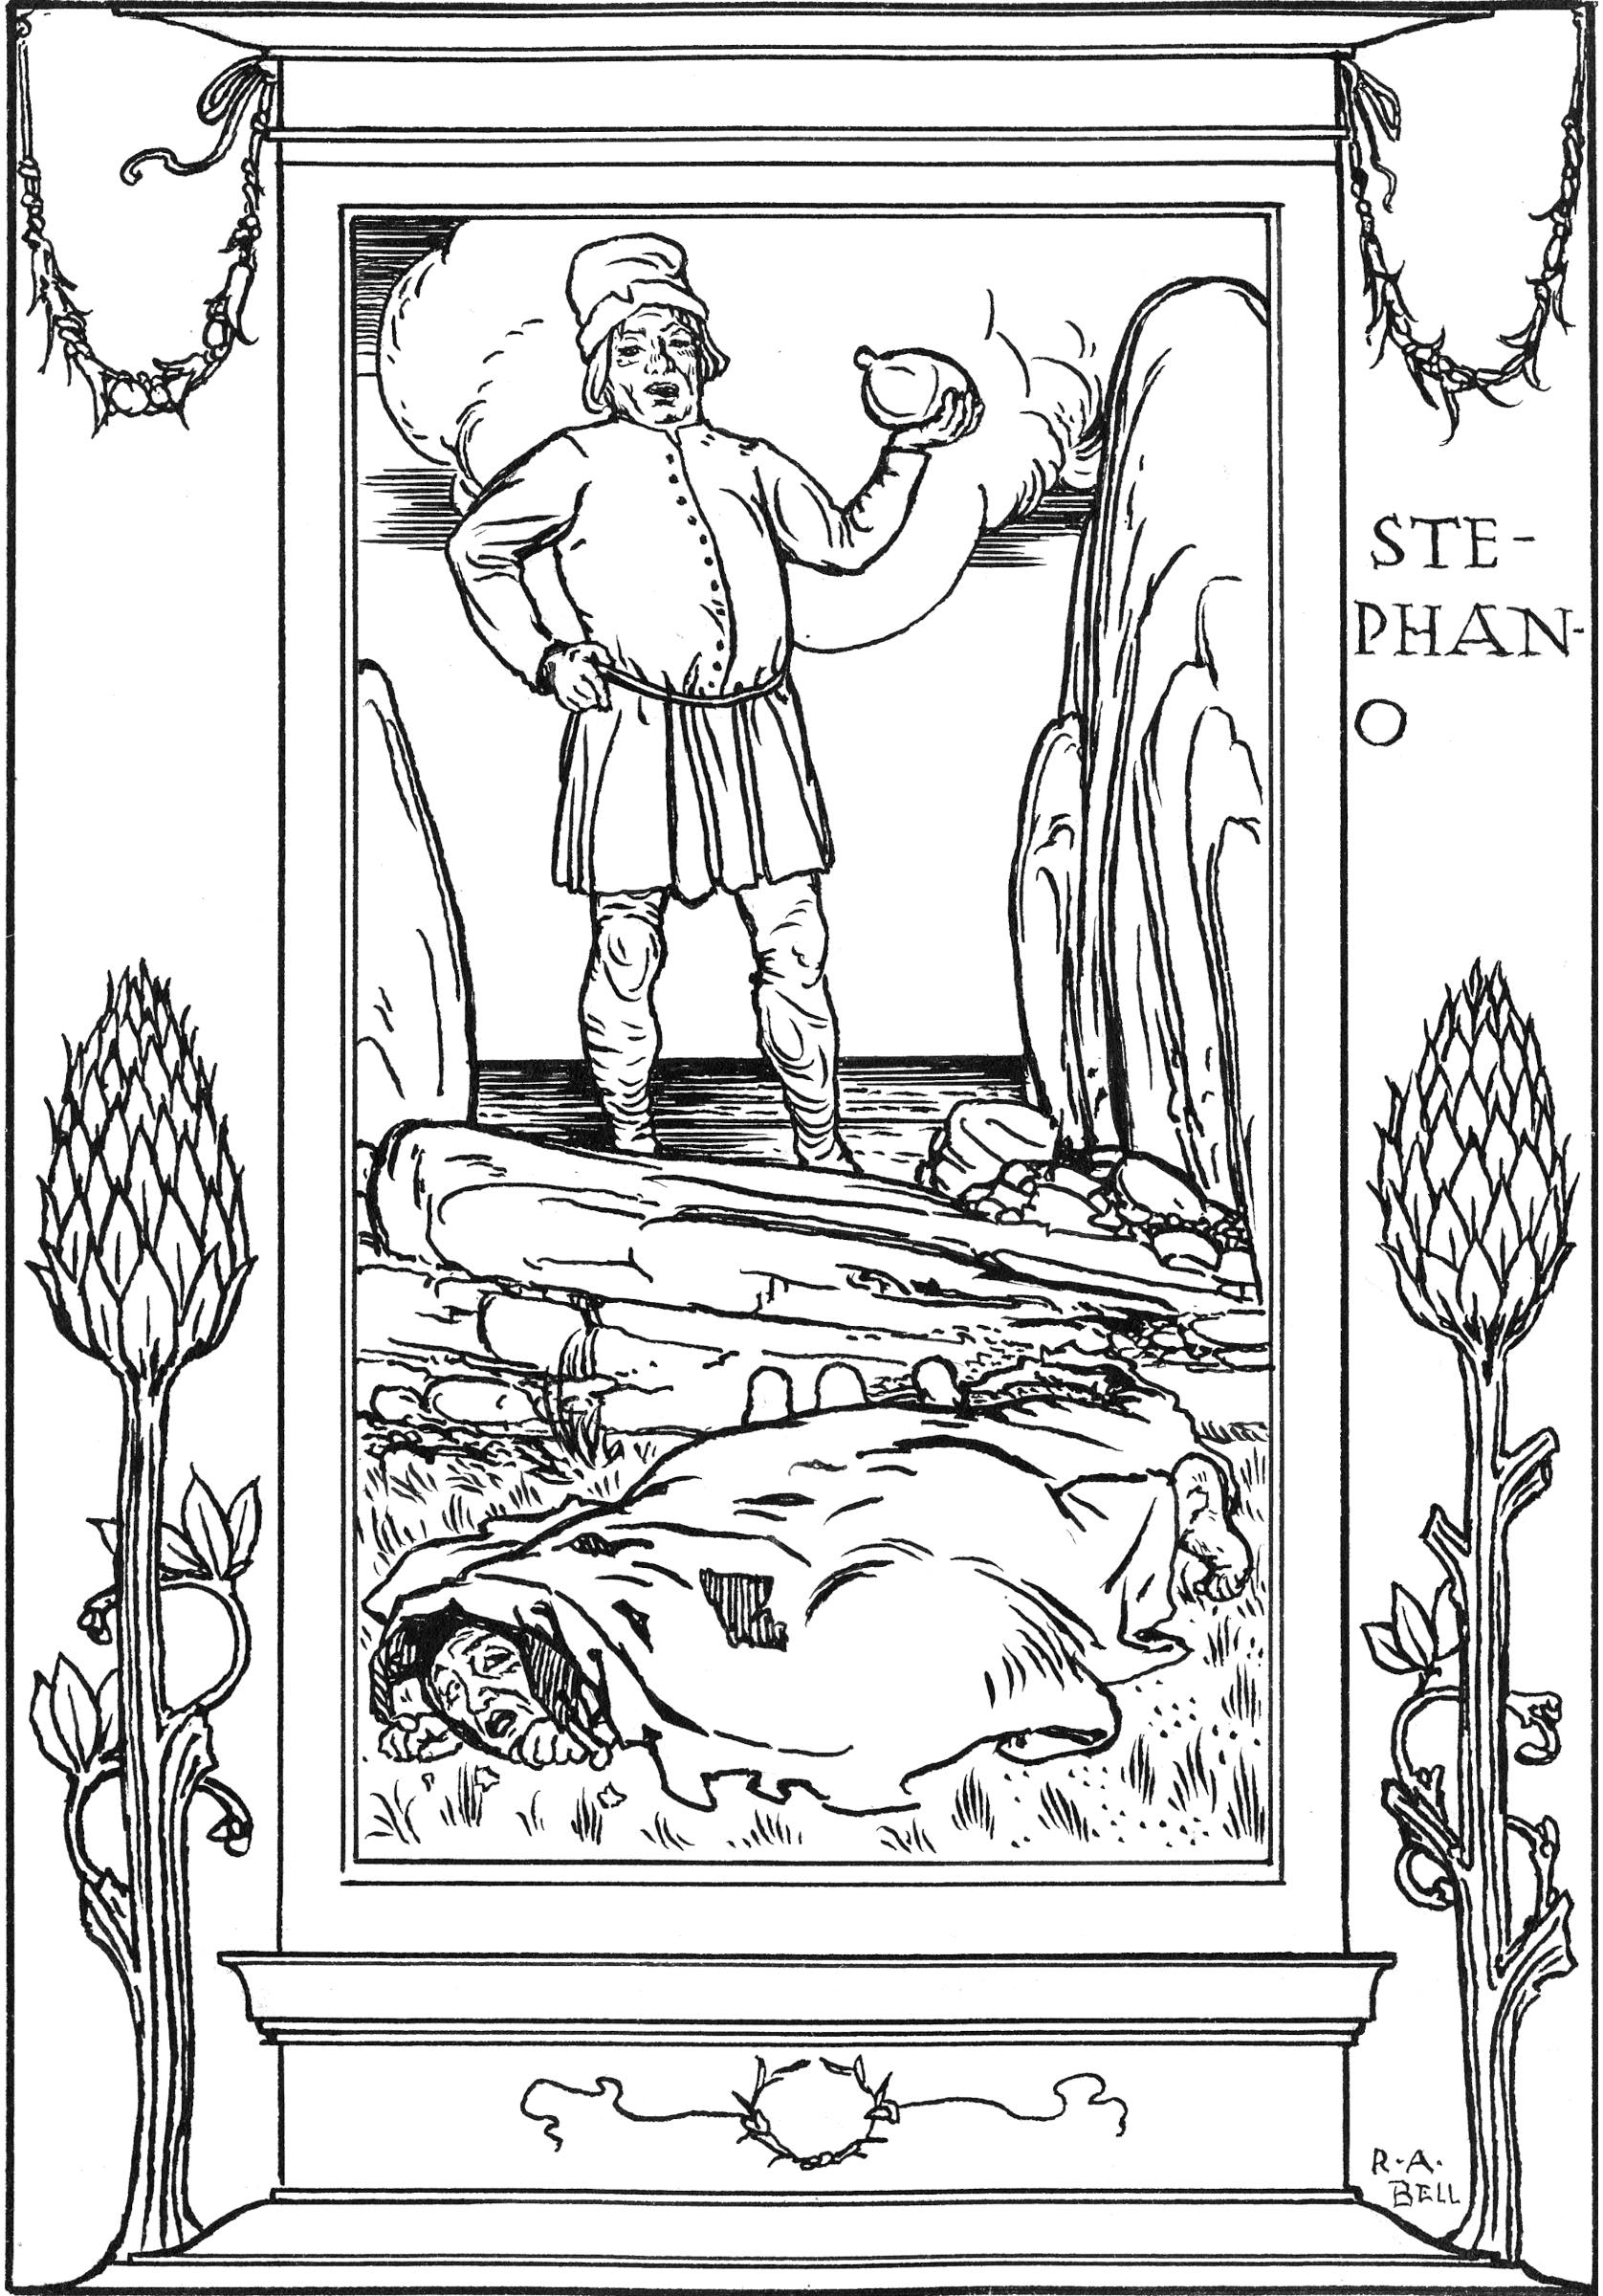
\includepdf[width=1.1\textwidth]{images/act2left.jpg}
		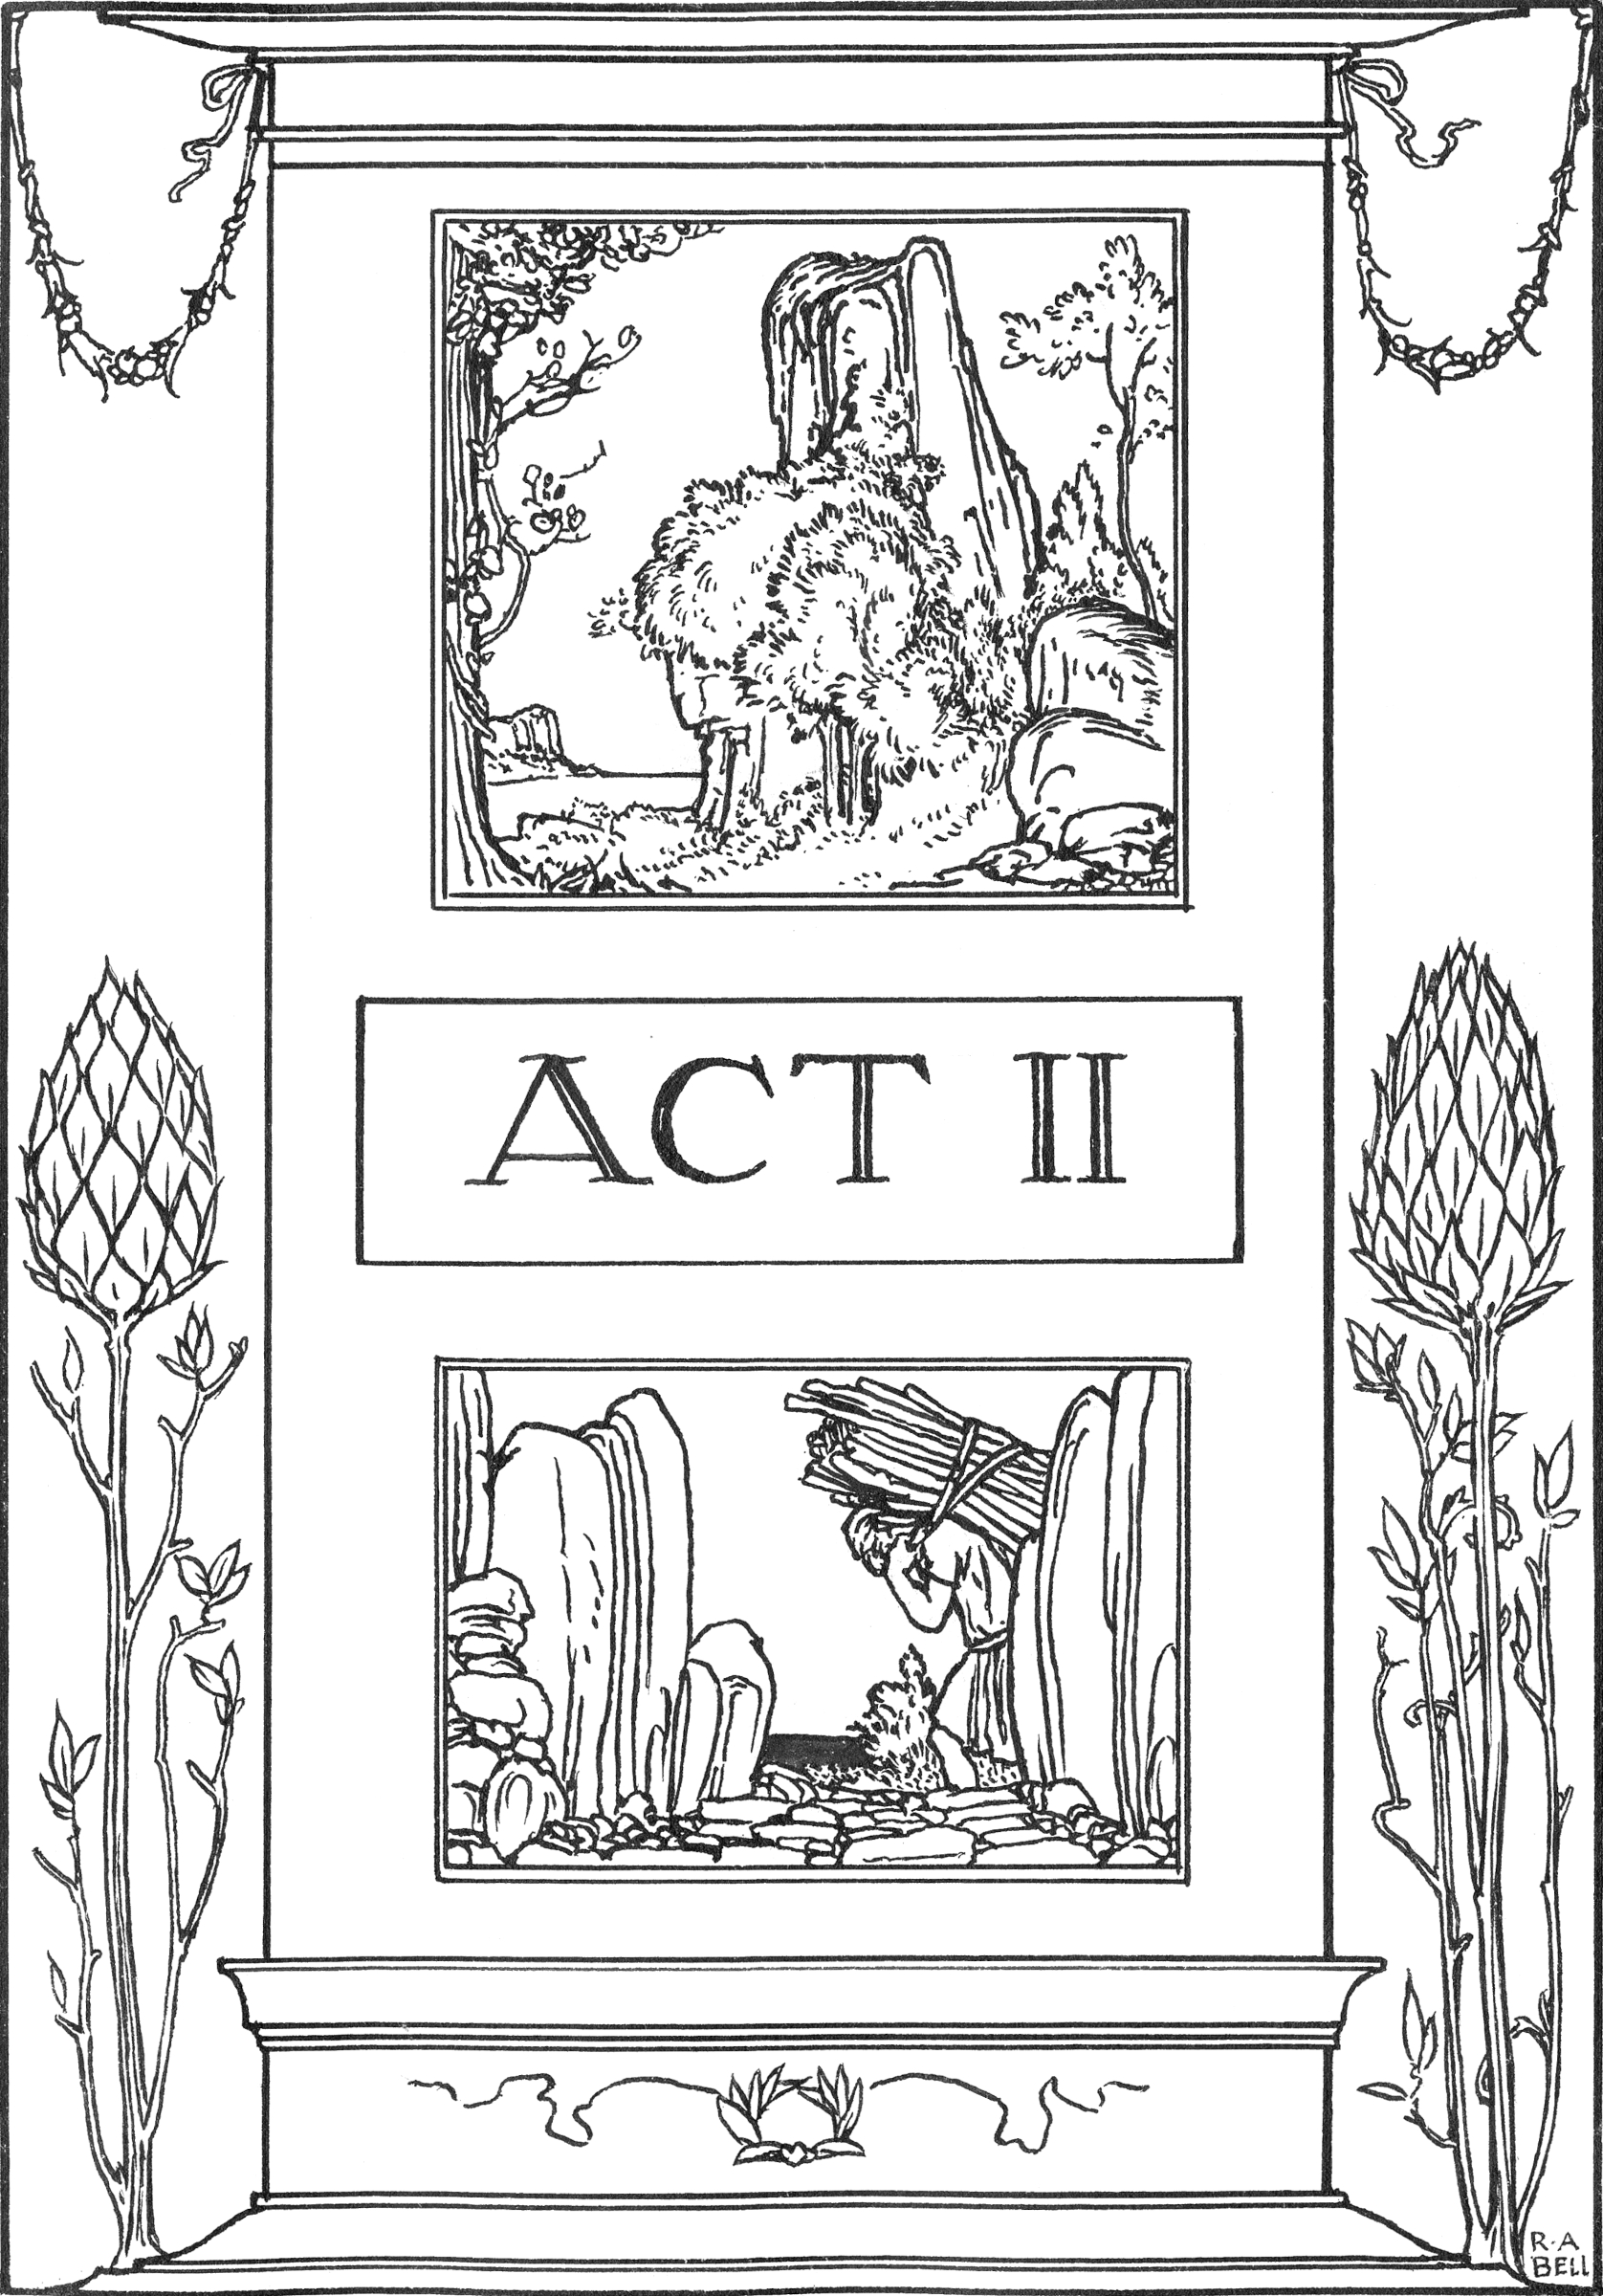
\includepdf[width=1.1\textwidth]{images/act2right.jpg}
	\end{letter}
	\begin{a4}
		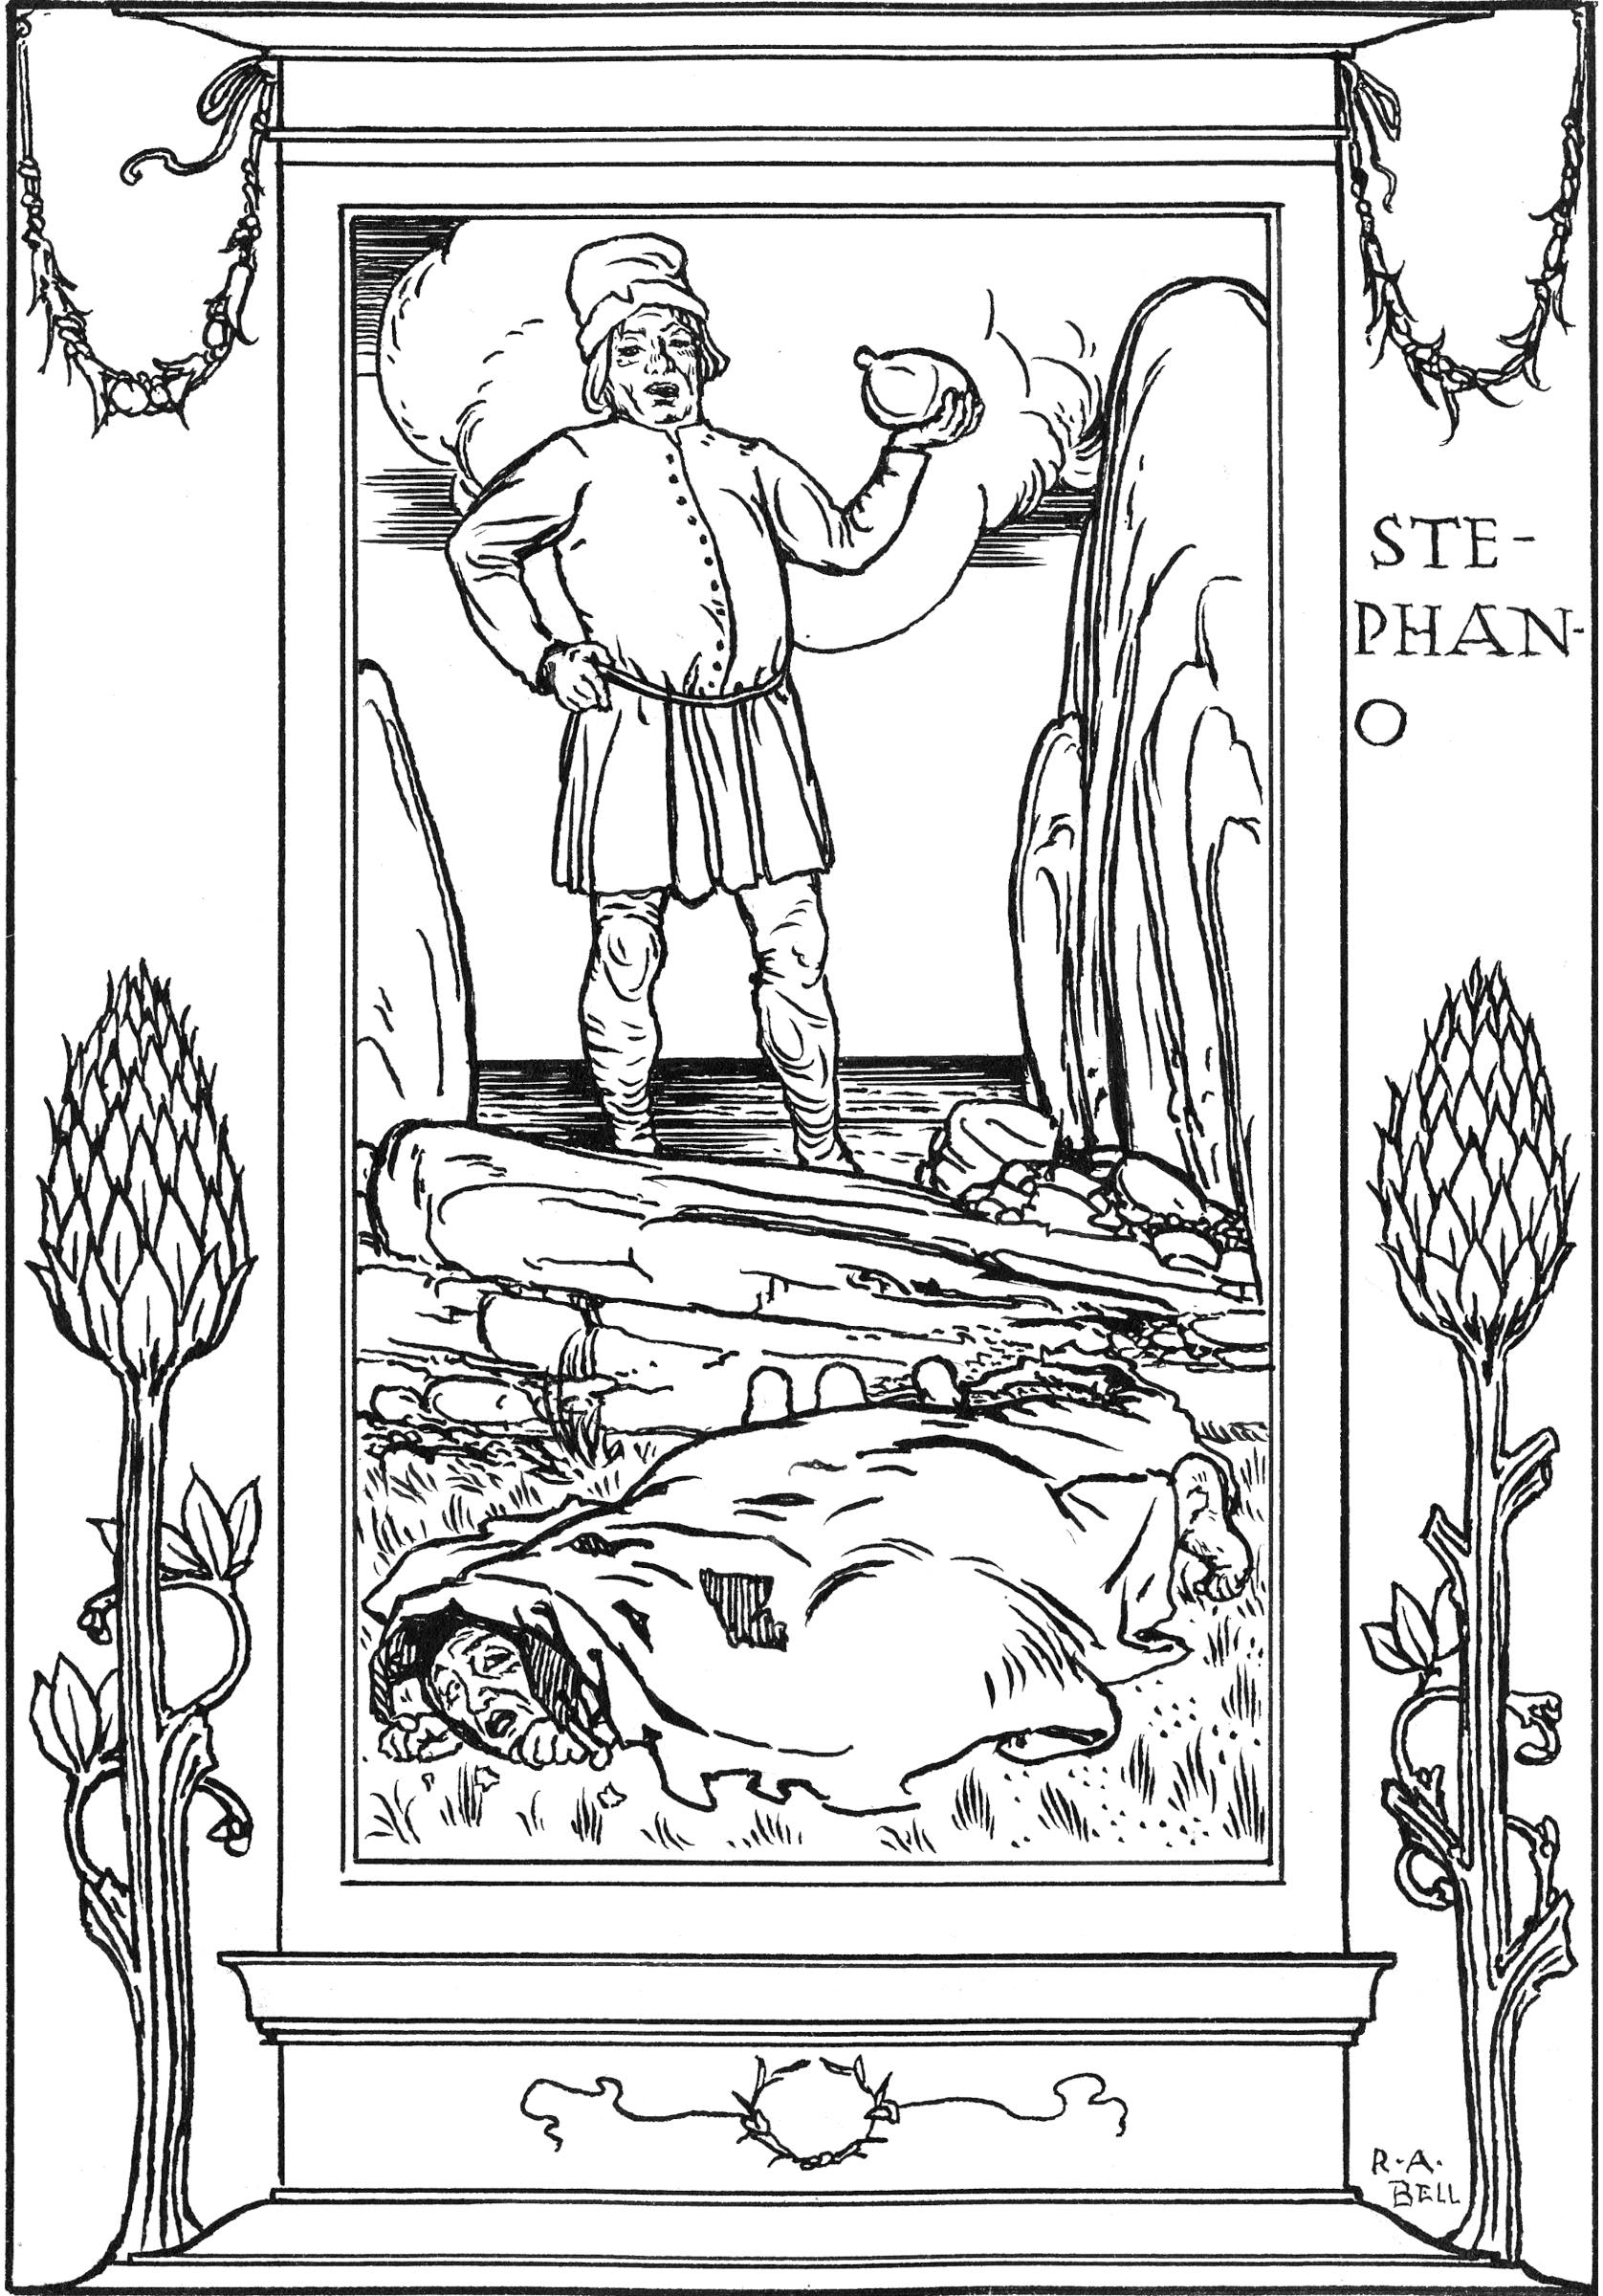
\includepdf[width=\textwidth]{images/act2left.jpg}
		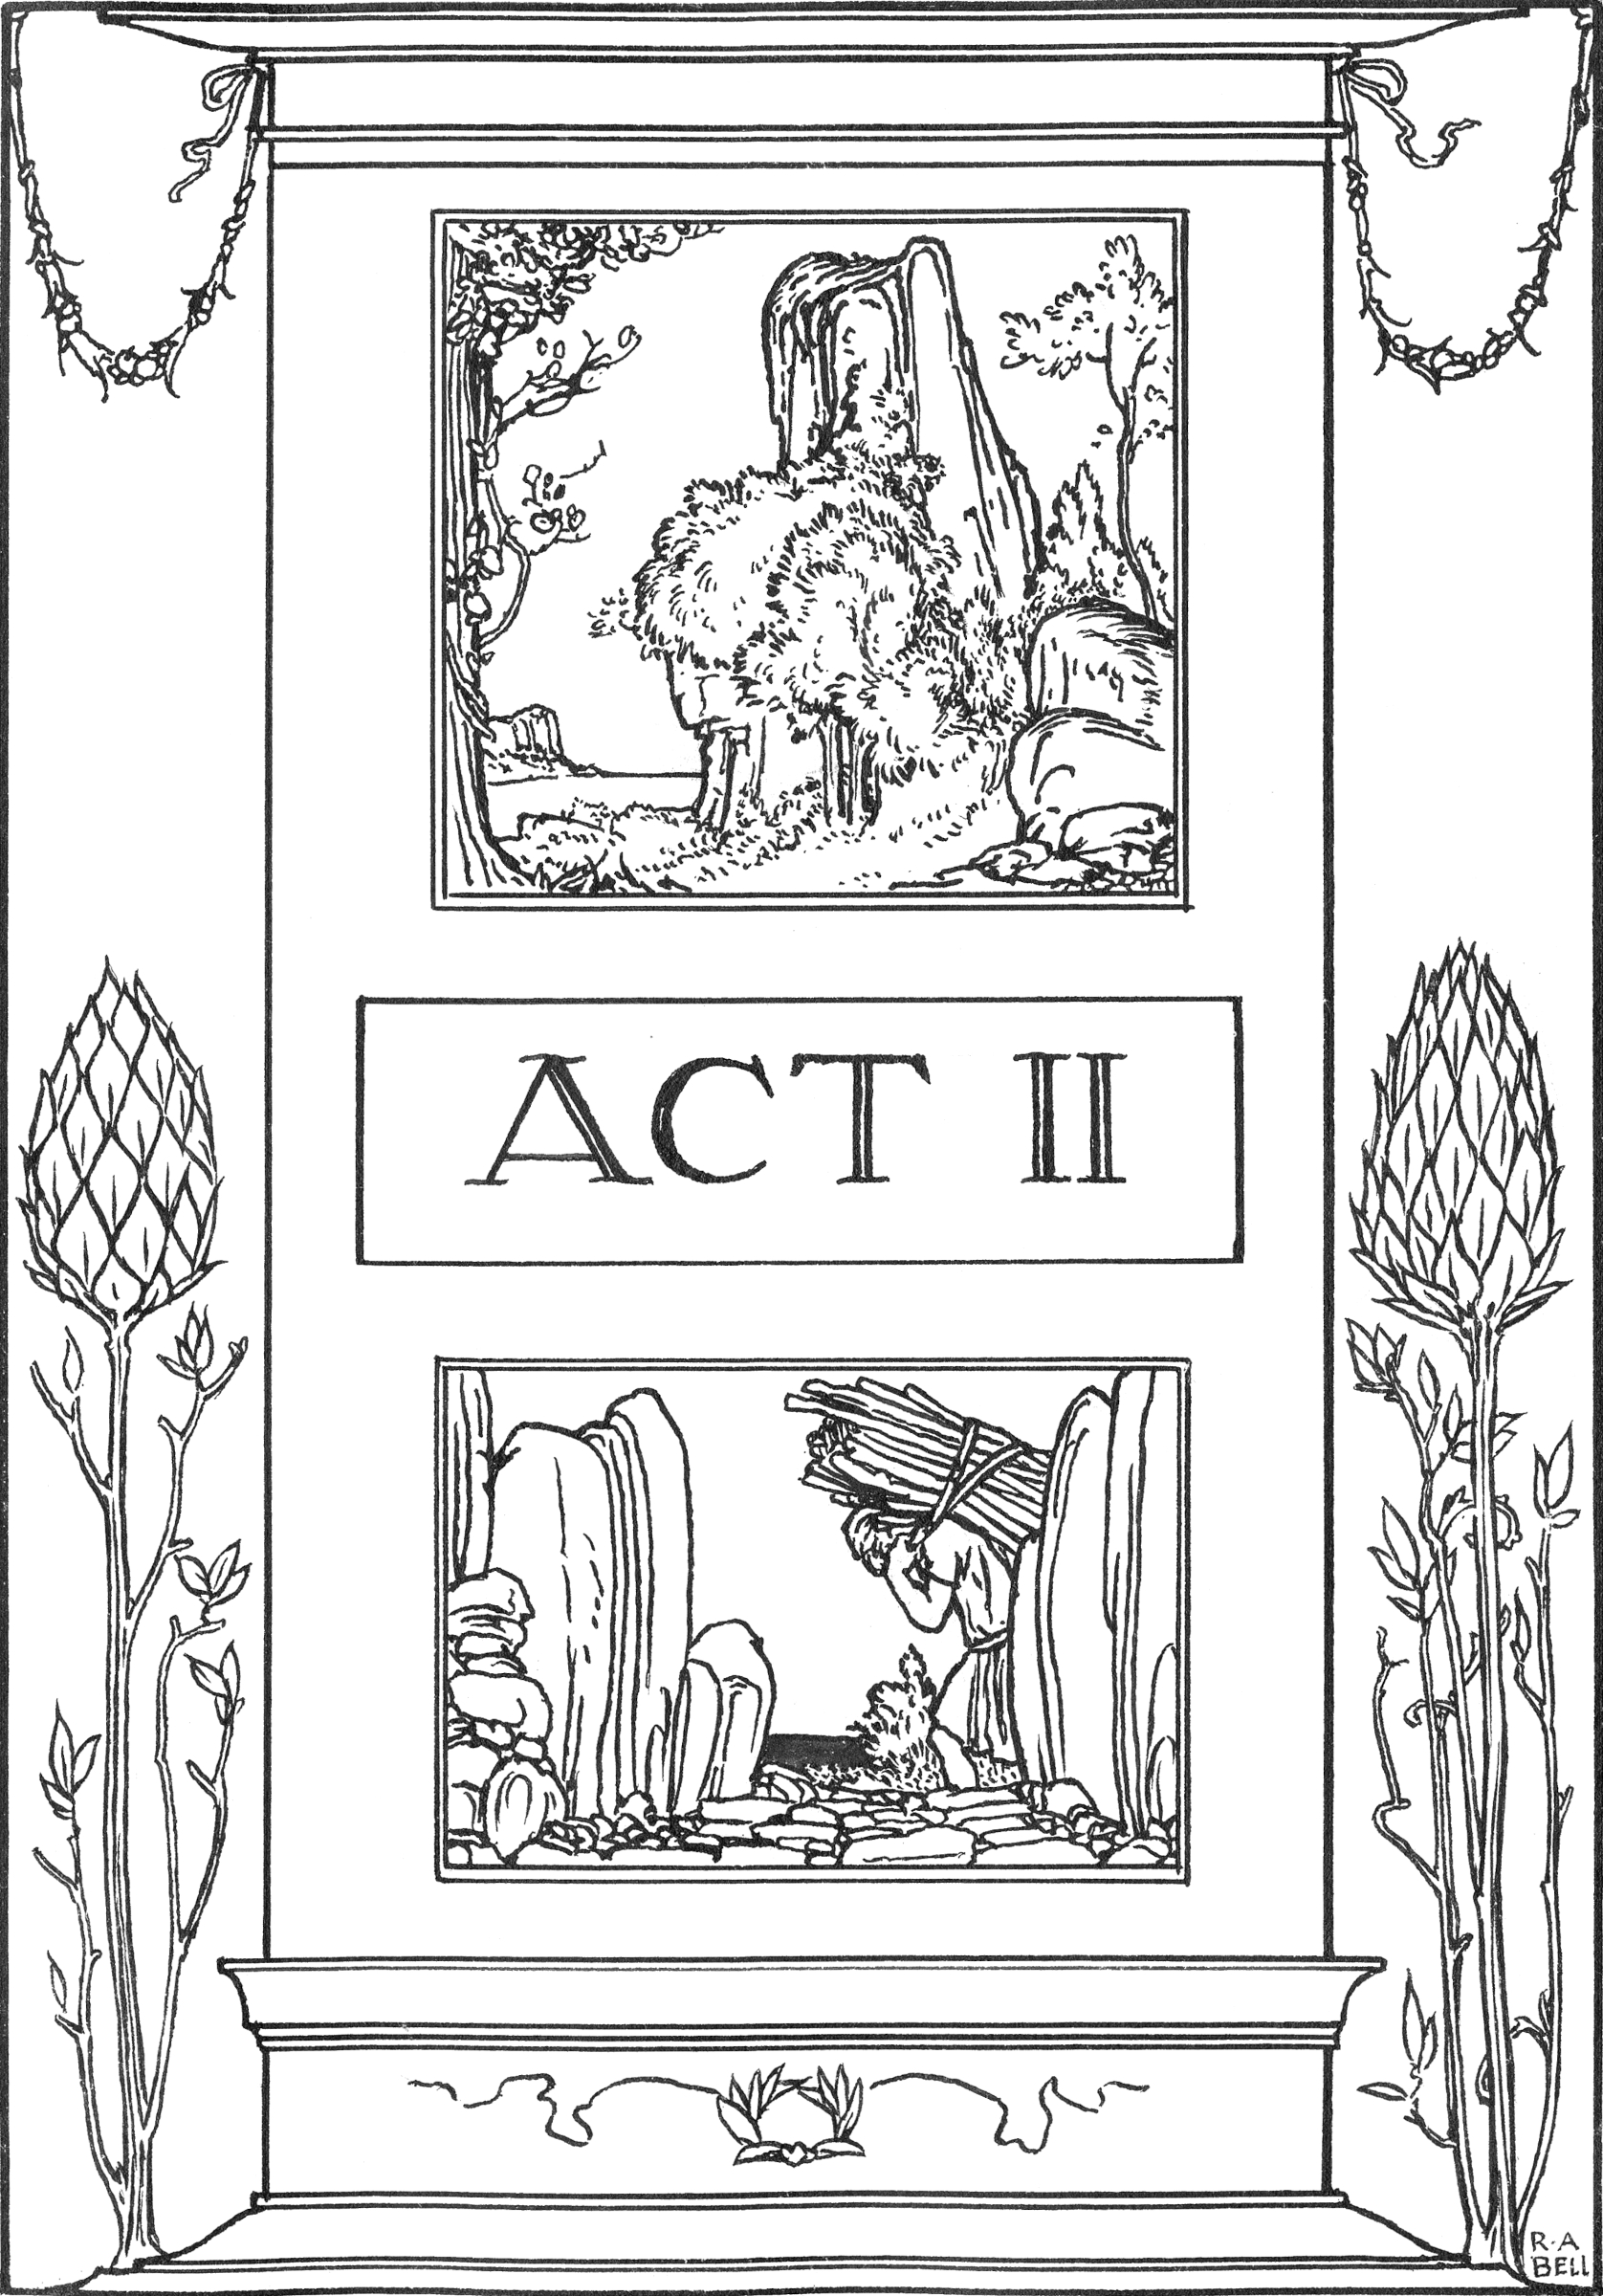
\includepdf[width=\textwidth]{images/act2right.jpg}
	\end{a4}
\end{pictures}
\begin{placeholder}
	\cleardoubleoddpage
\end{placeholder}



\cleardoubleoddpage
\Act*{2}
\Scene{1}[Another part of the island.]


\begin{letter}
	\begin{figure}[t!]
		\centering
		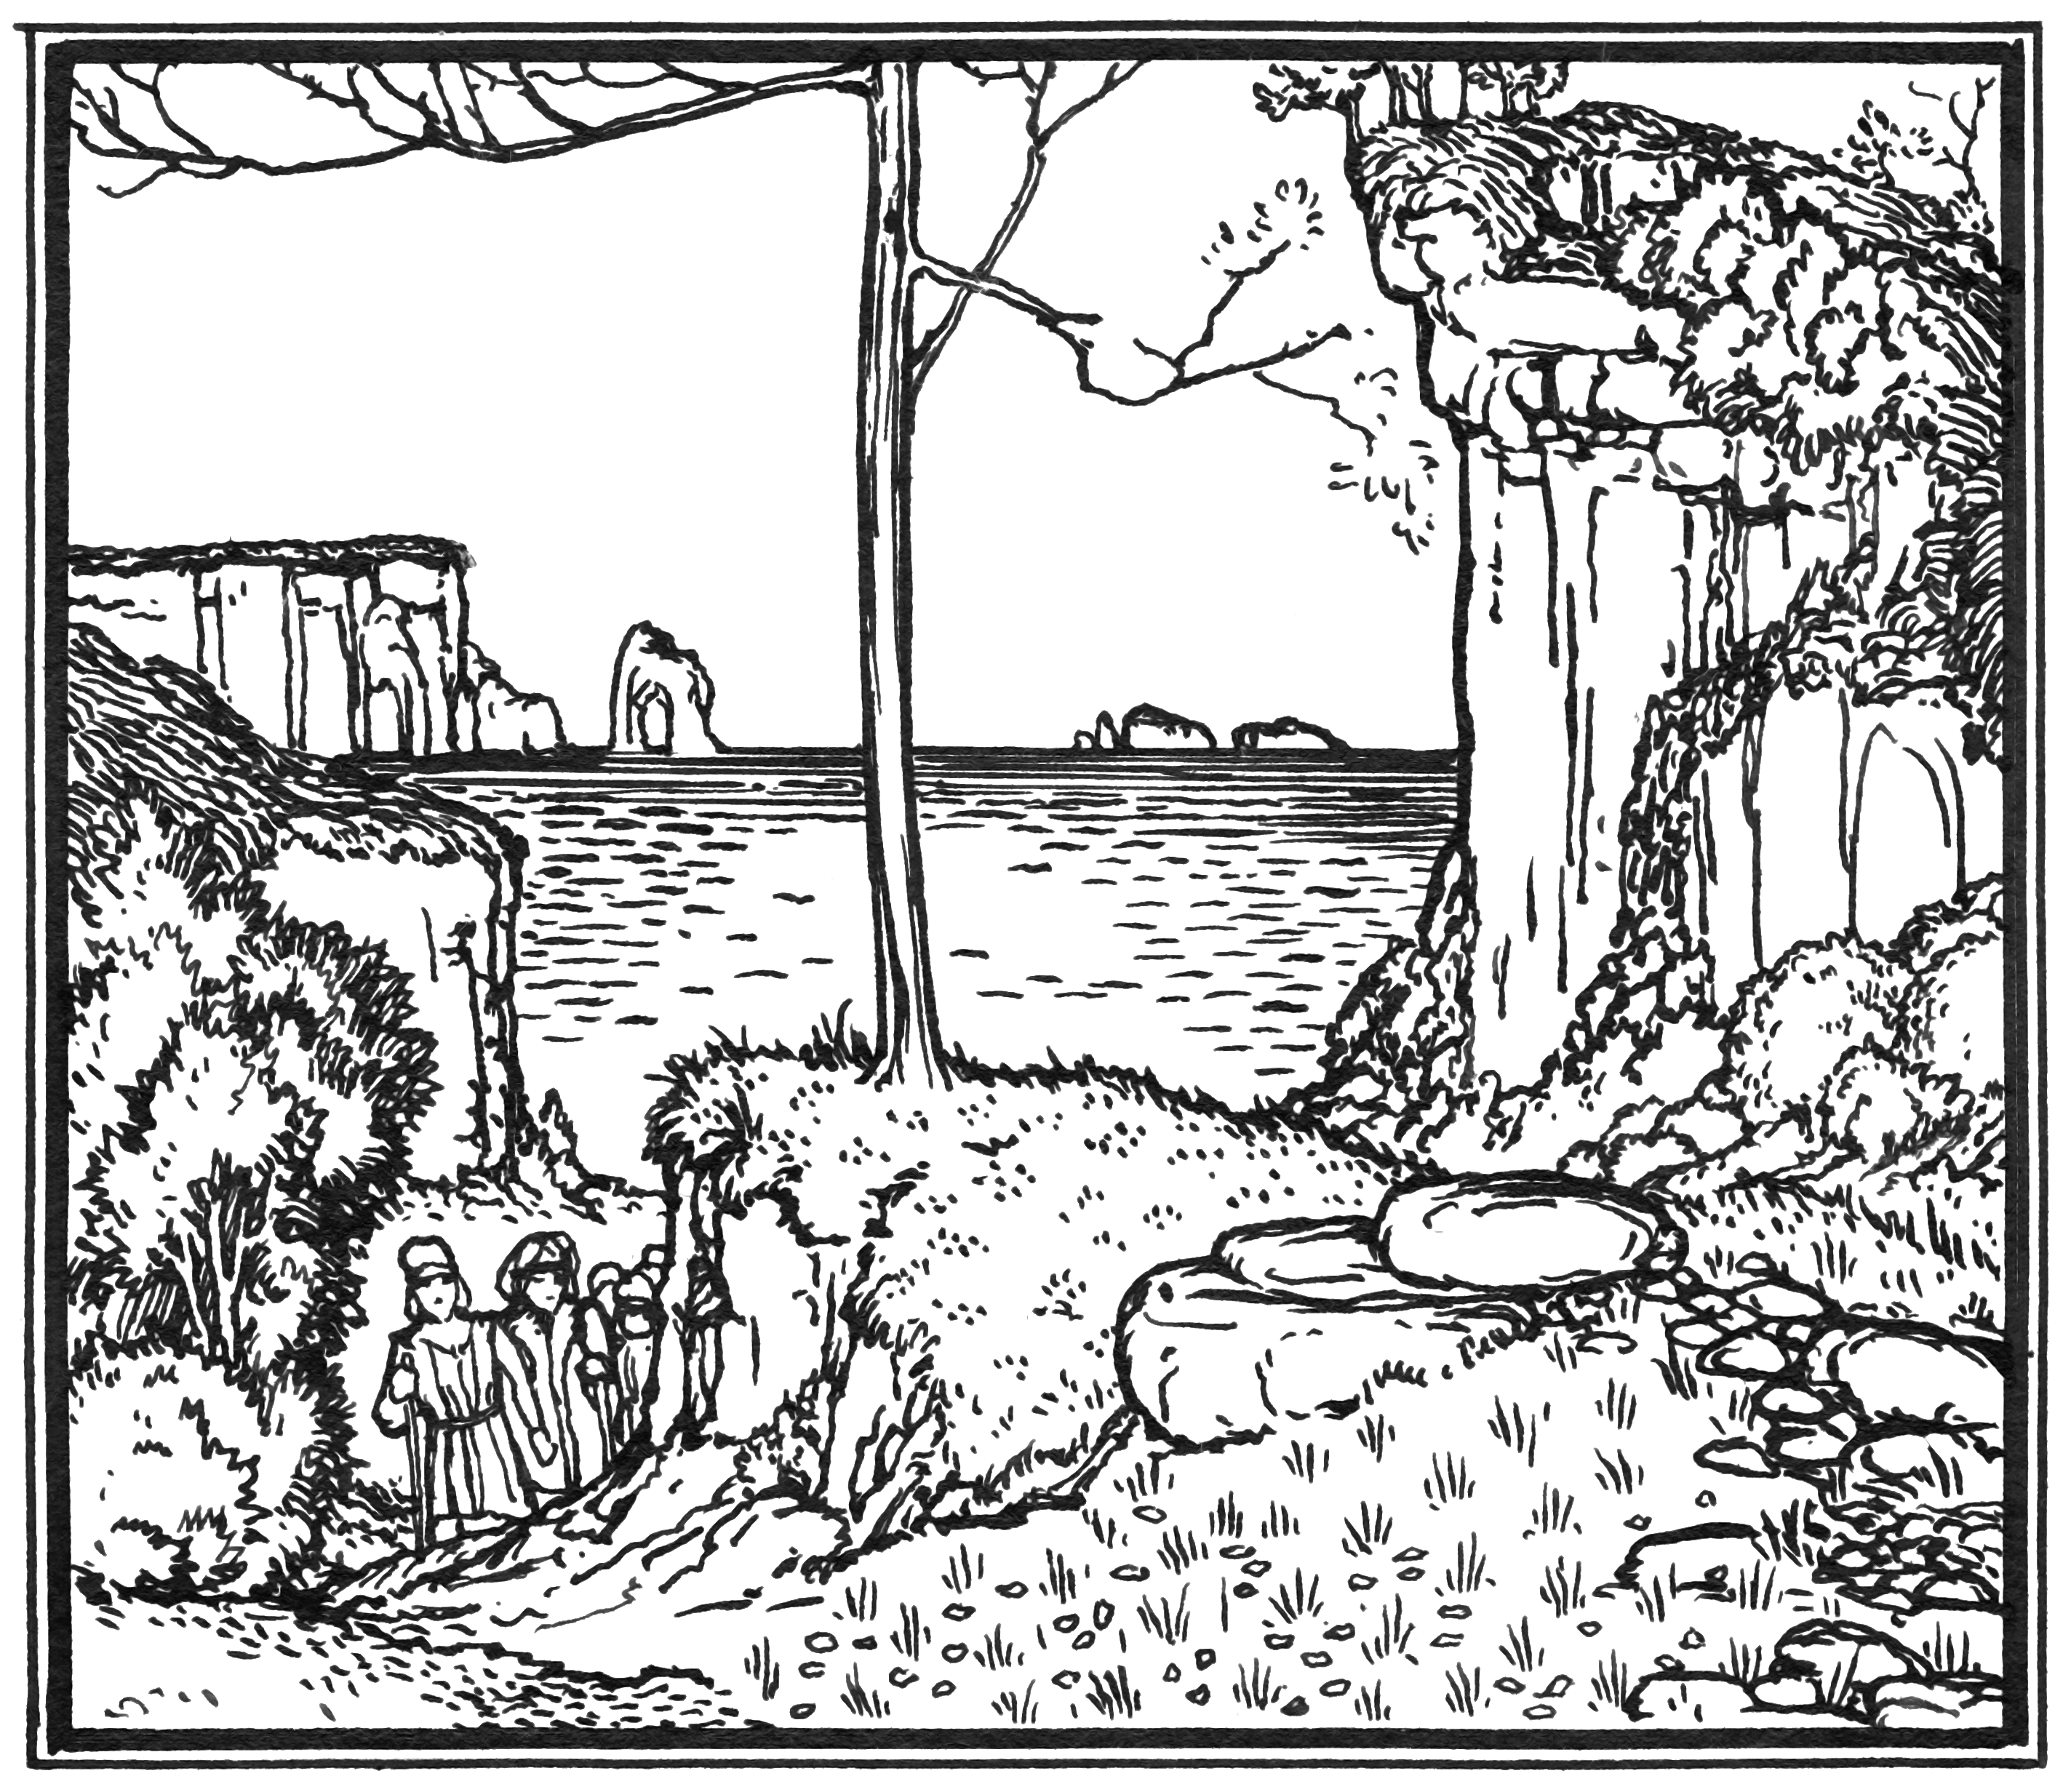
\includegraphics[width=0.9\textwidth]{2iheadpiece}
	\end{figure}
\end{letter}

\begin{a4}
	\begin{figure}[t!]
		\centering
		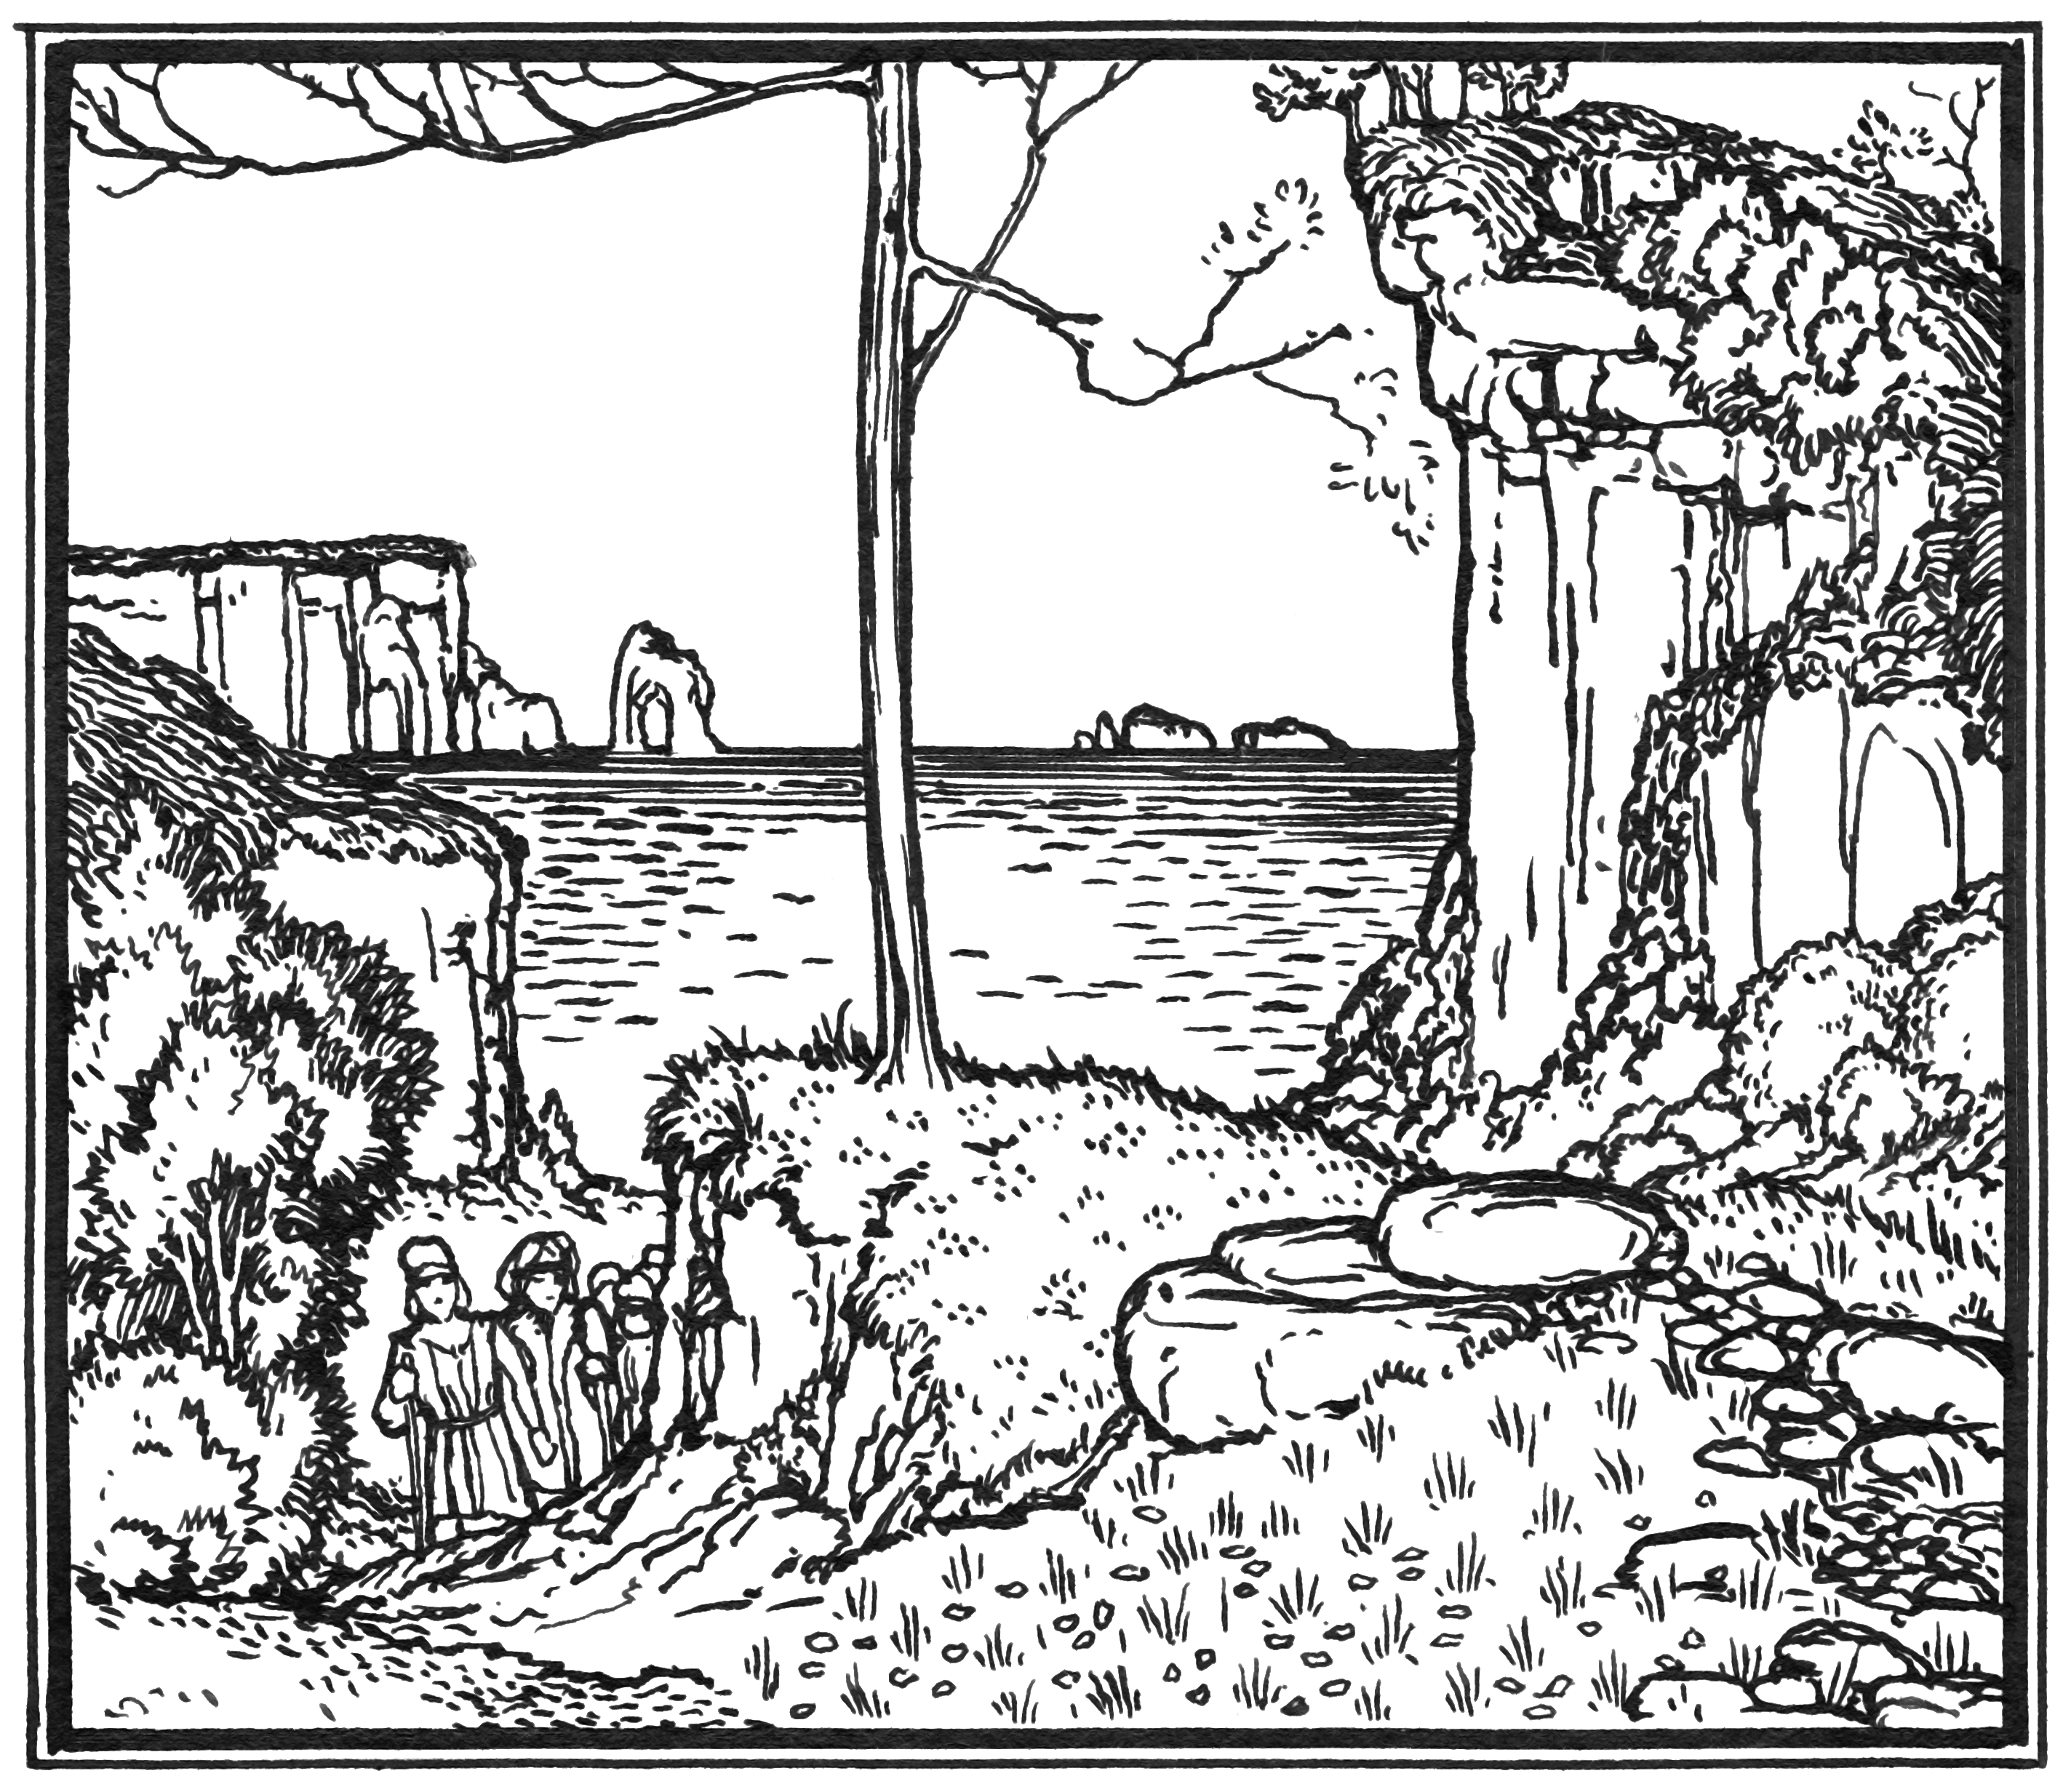
\includegraphics[width=0.8\textwidth]{2iheadpiece}
	\end{figure}
\end{a4}


\enter{\textsc{Alonso}, \textsc{Sebastian}, \textsc{Antonio}, \textsc{Gonzalo}, \textsc{Adrian}, \textsc{Francisco}, and others}

%dropcap
\begin{pictures}
\begin{letter}
	\begin{tikzpicture}[remember picture, overlay]
		\node (dropcap) at ($(current page.west)+(3cm,-4.75cm)$) {
\includegraphics[width=0.125\linewidth]{2idropcapB}};
	\end{tikzpicture}
		
	\begin{verse_speech}[Gonzalo] 
	\hspace{5em} \textit{(To \textsc{Alonso})}\\
	%\vspace*{3em}
	\hspace{2.5em} eseech you, sir, be merry; you have cause,\\
	\hspace{3em} So have we all, of joy; for our escape\\
	\hspace{3em} Is much beyond our loss. Our hint of woe\\
	Is common; every day some sailor's wife,\\
	The masters of some merchant and the merchant\\
	Have just our theme of woe; but for the miracle,\\
	I mean our preservation, few in millions\\
	Can speak like us: then wisely, good sir, weigh\\
	Our sorrow with our comfort.
	\end{verse_speech}
\end{letter}
\begin{a4}
	\begin{tikzpicture}[remember picture, overlay]
		\node (dropcap) at ($(current page.west)+(3.2cm,-5.8cm)$) {
\includegraphics[width=0.125\linewidth]{2idropcapB}};
	\end{tikzpicture}
		
	\begin{verse_speech}[Gonzalo] 
	\hspace{5em} \textit{(To \textsc{Alonso})}\\
	%\vspace*{3em}
	\hspace{3em} eseech you, sir, be merry; you have cause,\\
	\hspace{3em} So have we all, of joy; for our escape\\
	\hspace{3em} Is much beyond our loss. Our hint of woe\\
	Is common; every day some sailor's wife,\\
	The masters of some merchant and the merchant\\
	Have just our theme of woe; but for the miracle,\\
	I mean our preservation, few in millions\\
	Can speak like us: then wisely, good sir, weigh\\
	Our sorrow with our comfort.
	\end{verse_speech}
\end{a4}
\end{pictures}

\begin{placeholder}
	\begin{verse_speech}[Gonzalo] 
	\textit{(To \textsc{Alonso})}
	Beseech you, sir, be merry; you have cause,\\
	So have we all, of joy; for our escape\\
	Is much beyond our loss. Our hint of woe\\
	Is common; every day some sailor's wife,\\
	The masters of some merchant and the merchant\\
	Have just our theme of woe; but for the miracle,\\
	I mean our preservation, few in millions\\
	Can speak like us: then wisely, good sir, weigh\\
	Our sorrow with our comfort.
	\end{verse_speech}
\end{placeholder}

\verseline[Alonso]{Prithee, peace.} 
\verseline[Sebastian]{\asideto{Antonio}{He receives comfort like cold porridge.}}
\verseline[Antonio]{The visitor will not give him o'er so.} 
\begin{prose_speech}[Sebastian] Look he's winding up the watch of his wit; by and by it will strike.
\end{prose_speech}

\verseline[Gonzalo]{\textit{(To \textsc{Alonso})} 
Sir,—} 
\verseline[Sebastian]{One: tell.} 
\begin{verse_speech}[Gonzalo] When every grief is entertain'd that's offer'd,\\
Comes to the entertainer—
\end{verse_speech}

\verseline[Sebastian]{A dollar.} 
\begin{prose_speech}[Gonzalo] Dolour comes to him, indeed: you have spoken truer than you purposed.
\end{prose_speech}

\verseline[Sebastian]{You have taken it wiselier than I meant you should.} 
\verseline[Gonzalo]{\textit{(To \textsc{Alonso})} 
Therefore, my lord,—} 
\verseline[Antonio]{Fie, what a spendthrift is he of his tongue!} 
\verseline[Alonso]{\textit{(To \textsc{Gonzalo})} 
I prithee, spare.} 
\verseline[Gonzalo]{Well, I have done: but yet,—} 
\verseline[Sebastian]{\asideto{Antonio}{He will be talking.} }
\begin{prose_speech}[Antonio] 
\asideto{Sebastian}{Which, of he or Adrian, for a good wager, first begins to crow?}
\end{prose_speech}

\verseline[Sebastian]{The old cock.} 
\verseline[Antonio]{The cockerel.} 
\verseline[Sebastian]{Done. The wager?} 
\verseline[Antonio]{A laughter.} 
\verseline[Sebastian]{A match!} 
\verseline[Adrian]{Though this island seem to be desert,—} 
\verseline[Sebastian]{Ha, ha, ha! So, you're paid.} 
\verseline[Adrian]{Uninhabitable and almost inaccessible,—} 
\verseline[Sebastian]{Yet,—} 
\verseline[Adrian]{Yet,—} 
\verseline[Antonio]{He could not miss't.} 
\verseline[Adrian]{It must needs be of subtle, tender and delicate temperance.}
\verseline[Antonio]{Temperance was a delicate wench.} 
\verseline[Sebastian]{Ay, and a subtle; as he most learnedly delivered.} 
\verseline[Adrian]{The air breathes upon us here most sweetly.} 
\verseline[Sebastian]{As if it had lungs and rotten ones.} 
\verseline[Antonio]{Or as 'twere perfumed by a fen.} 
\verseline[Gonzalo]{Here is everything advantageous to life.} 
\verseline[Antonio]{True; save means to live.} 
\verseline[Sebastian]{Of that there's none, or little.} 
\verseline[Gonzalo]{How lush and lusty the grass looks! how green!} 
\verseline[Antonio]{The ground indeed is tawny.} 
\verseline[Sebastian]{With an eye of green in't.} 
\verseline[Antonio]{He misses not much.} 
\verseline[Sebastian]{No; he doth but mistake the truth totally.} 
\verseline[Gonzalo]{But the rarity of it is,—which is indeed almost} 
beyond credit,—
\verseline[Sebastian]{As many vouched rarities are.} 
\begin{prose_speech}[Gonzalo] That our garments, being, as they were, drenched in the sea, hold notwithstanding their freshness and glosses, being rather new-dyed than stained with salt water.
\end{prose_speech}

\verseline[Antonio]{If but one of his pockets could speak, would it not say he lies?}
\verseline[Sebastian]{Ay, or very falsely pocket up his report} 
\begin{prose_speech}[Gonzalo] Methinks our garments are now as fresh as when we put them on first in Afric, at the marriage of the king's fair daughter Claribel to the King of Tunis.
\end{prose_speech}

\begin{figure}[tb]
\centering
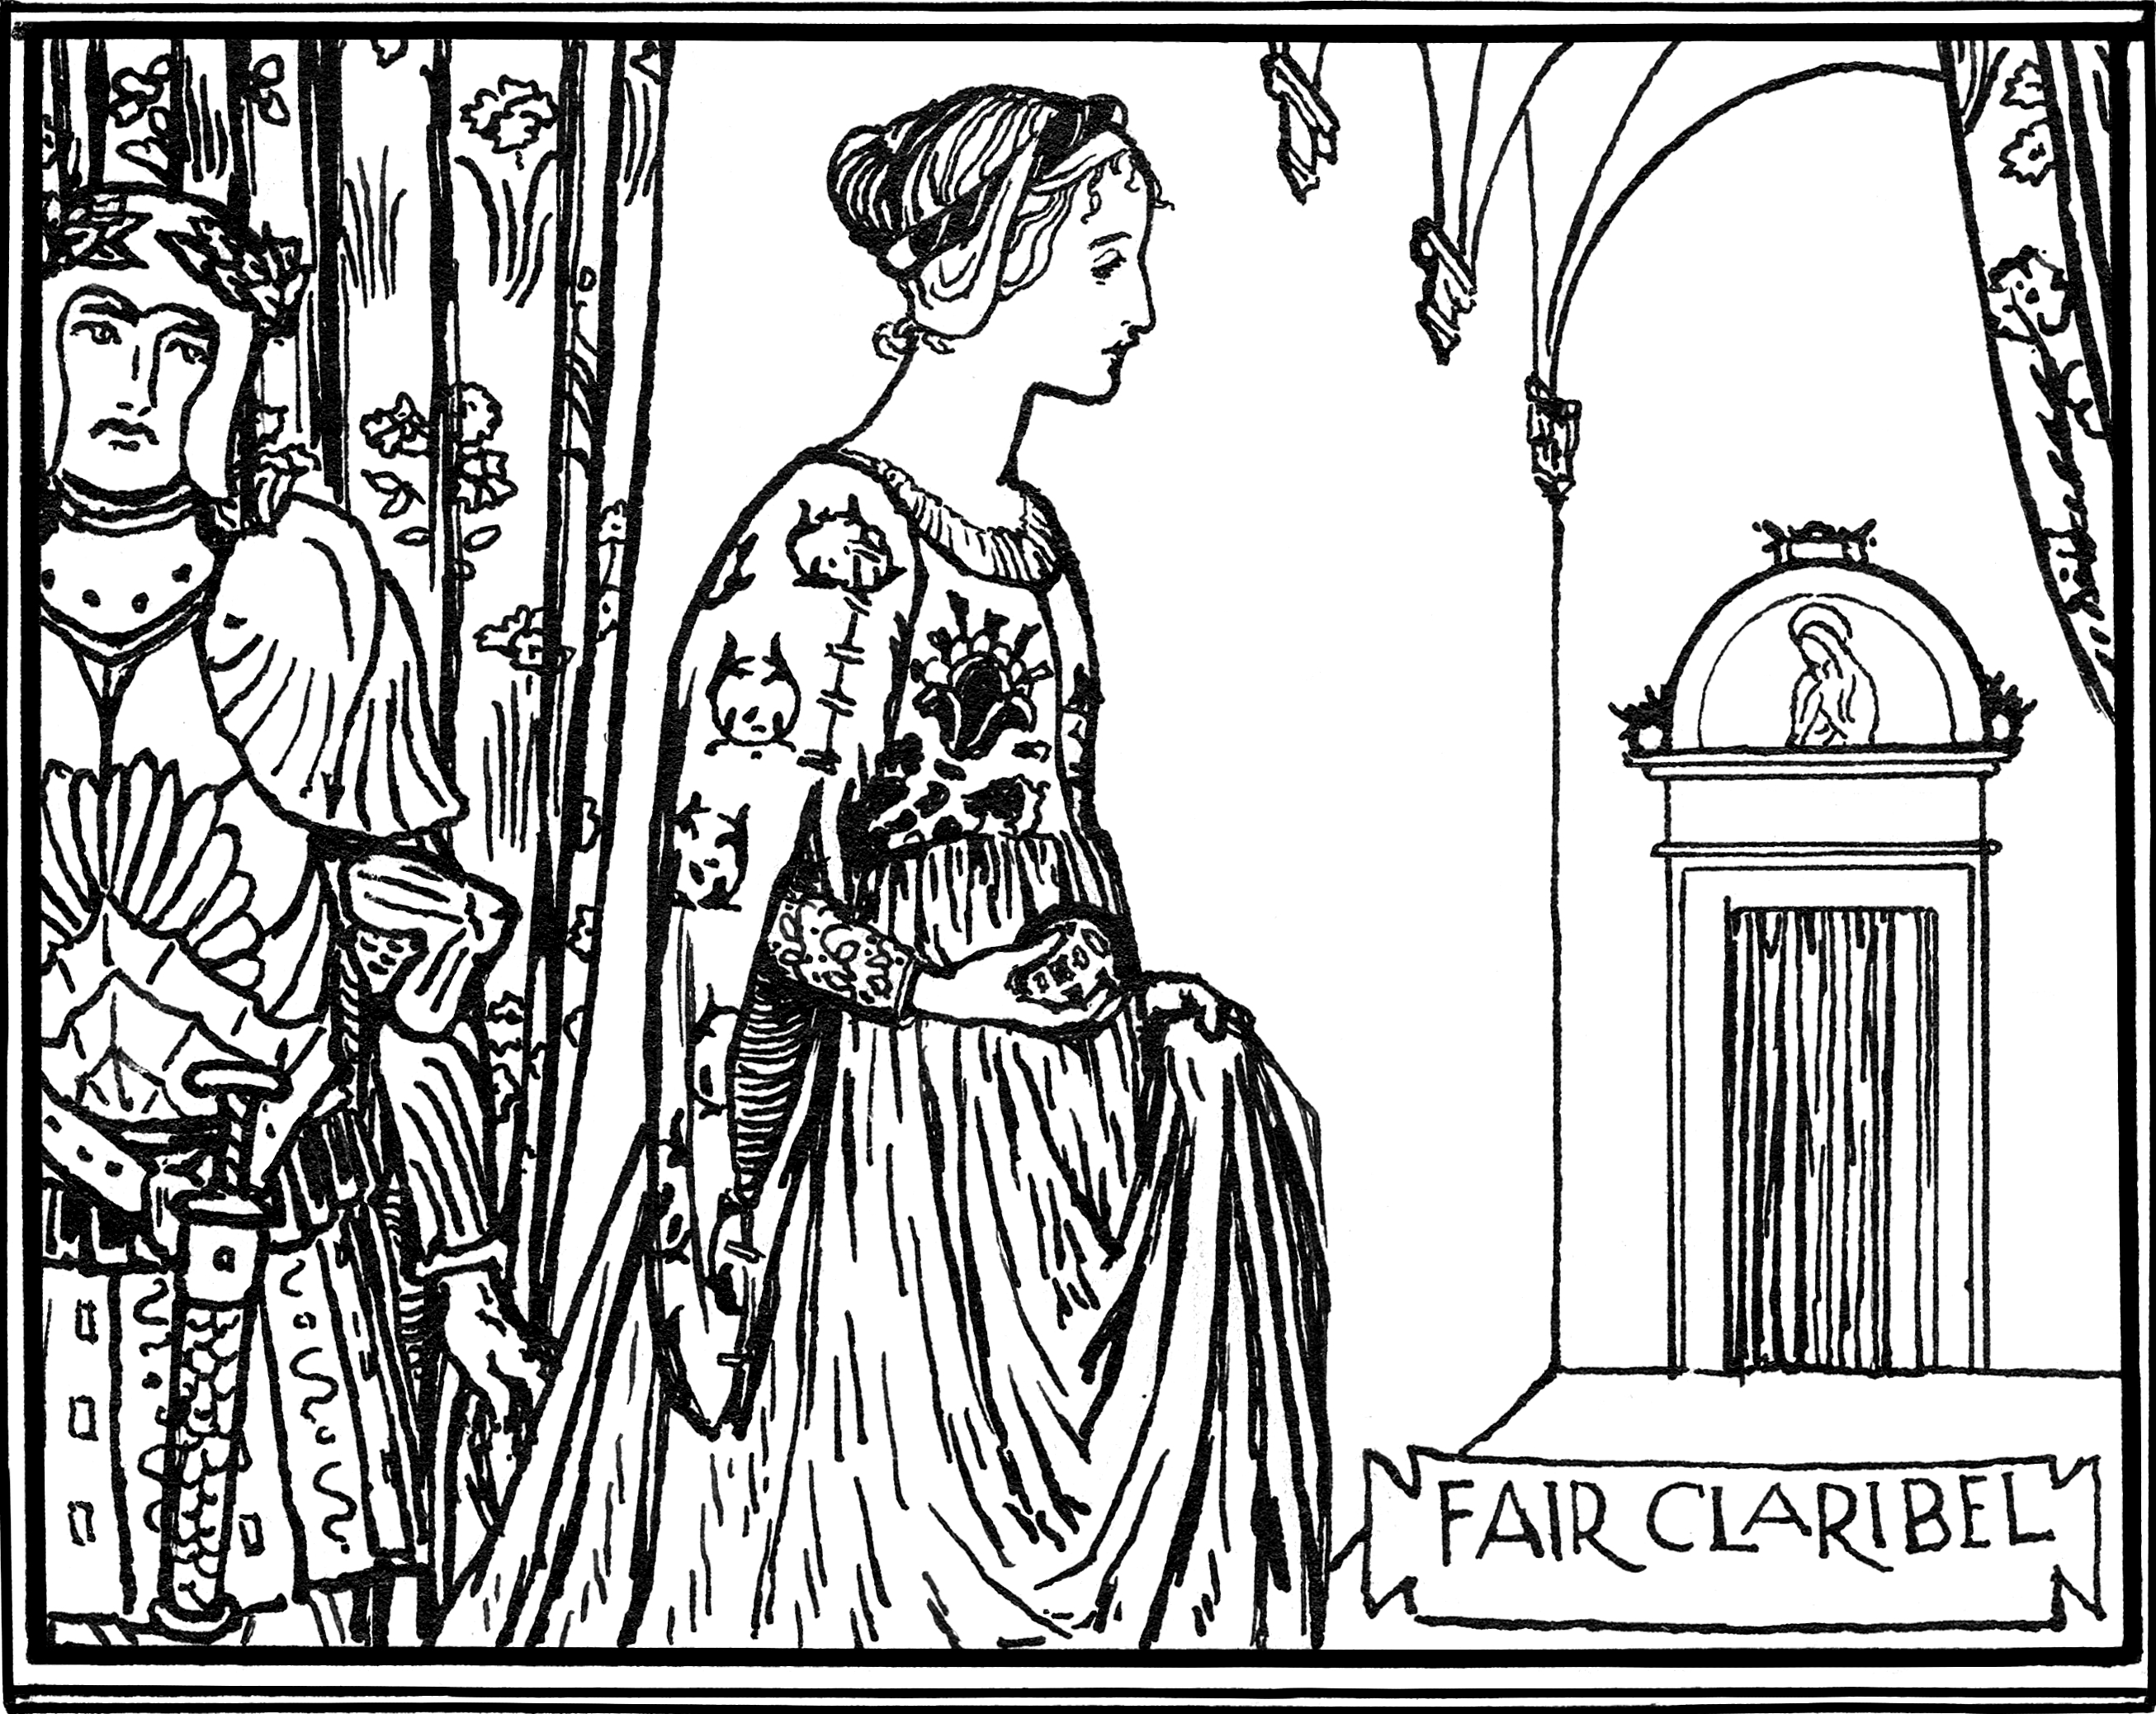
\includegraphics[width=0.8\textwidth]{2ifairclaribel}
\end{figure}

\begin{figure}[tb]
\centering
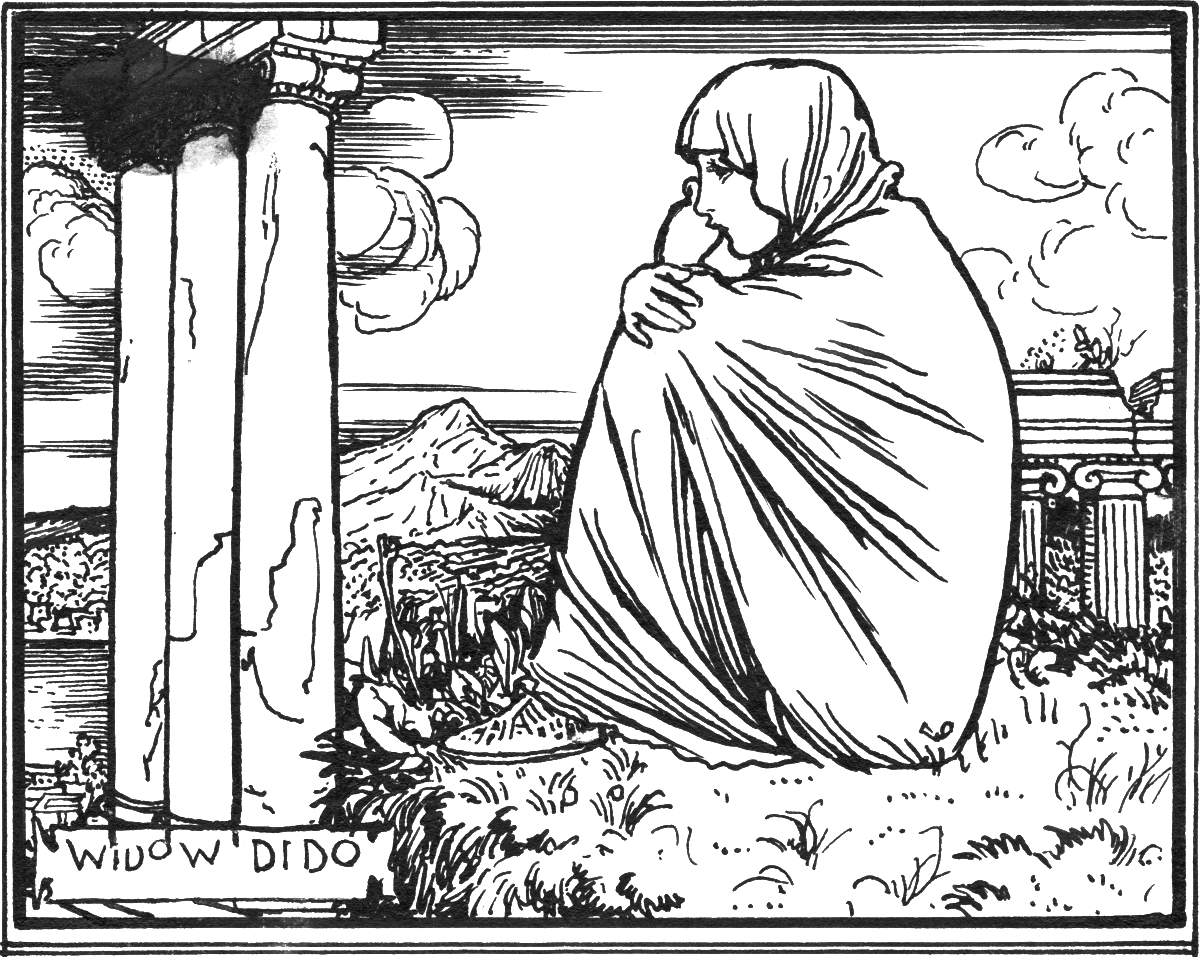
\includegraphics[width=0.8\textwidth]{2iwidow}
\end{figure}

\verseline[Sebastian]{'Twas a sweet marriage, and we prosper well in our return.} 
\verseline[Adrian]{Tunis was never graced before with such a paragon to} 
their queen.
\verseline[Gonzalo]{Not since widow Dido's time.} 
\verseline[Antonio]{Widow! a pox o' that! How came that widow in? widow Dido!}
\verseline[Sebastian]{What if he had said <widower Æneas> too? Good Lord,
how you take it!}
\verseline[Adrian]{\textit{(To \textsc{Gonzalo})} <Widow Dido> said you? you make me study of that: she was of Carthage, not of Tunis.}
\verseline[Gonzalo]{This Tunis, sir, was Carthage.} 
\verseline[Adrian]{Carthage?} 
\verseline[Gonzalo]{I assure you, Carthage.} 
\verseline[Sebastian]{His word is more than the miraculous harp; he hath} 
raised the wall and houses too.
\verseline[Antonio]{What impossible matter will he make easy next?} 
\verseline[Sebastian]{I think he will carry this island home in his pocket} 
and give it his son for an apple.
\verseline[Antonio]{And, sowing the kernels of it in the sea, bring} 
forth more islands.
\verseline[Gonzalo]{Ay.} 
\verseline[Antonio]{Why, in good time.} 
\verseline[Gonzalo]{\textit{(To \textsc{Alonso})} Sir, we were talking that our garments seem now} 
as fresh as when we were at Tunis at the marriage
of your daughter, who is now queen.
\verseline[Antonio]{And the rarest that e'er came there.} 
\verseline[Sebastian]{Bate, I beseech you, widow Dido.} 
\verseline[Antonio]{O, widow Dido! ay, widow Dido.} 
\verseline[Gonzalo]{\textit{(To \textsc{Alonso})} Is not, sir, my doublet as fresh as the first day I wore it? I mean, in a sort.}
\verseline[Antonio]{That sort was well fished for.} 
\verseline[Gonzalo]{\textit{(To \textsc{Alonso})} When I wore it at your daughter's marriage?} 
\begin{verse_speech}[Alonso] 
You cram these words into mine ears against\\
The stomach of my sense. Would I had never\\
Married my daughter there! for, coming thence,\\
My son is lost and, in my rate, she too,\\
Who is so far from Italy removed\\
I ne'er again shall see her. O thou mine heir\\
Of Naples and of Milan, what strange fish\\
Hath made his meal on thee?
\end{verse_speech}

\begin{verse_speech}[Francisco] 
Sir, he may live:\\
I saw him beat the surges under him,\\
And ride upon their backs; he trod the water,\\
Whose enmity he flung aside, and breasted\\
The surge most swoln that met him; his bold head\\
'Bove the contentious waves he kept, and oar'd\\
Himself with his good arms in lusty stroke\\
To the shore, that o'er his wave-worn basis bow'd,\\
As stooping to relieve him: I not doubt\\
He came alive to land.
\end{verse_speech}

\verseline[Alonso]{No, no, he's gone.} 
\begin{verse_speech}[Sebastian] 
Sir, you may thank yourself for this great loss,\\
That would not bless our Europe with your daughter,\\
But rather lose her to an African;\\
Where she at least is banish'd from your eye,\\
Who hath cause to wet the grief on't.
\end{verse_speech}

\verseline[Alonso]{Prithee, peace.} 
\begin{verse_speech}[Sebastian] 
You were kneel'd to and importuned otherwise\\
By all of us, and the fair soul herself\\
Weigh'd between loathness and obedience, at\\
Which end o' the beam should bow. We have lost your son,\\
I fear, for ever: Milan and Naples have\\
More widows in them of this business' making\\
Than we bring men to comfort them:\\
The fault's your own.
\end{verse_speech}

\verseline[Alonso]{So is the dear'st o' the loss.} 
\begin{verse_speech}[Gonzalo] My lord Sebastian,\\
The truth you speak doth lack some gentleness\\
And time to speak it in: you rub the sore,\\
When you should bring the plaster.
\end{verse_speech}

\verseline[Sebastian]{Very well.} 
\verseline[Antonio]{And most chirurgeonly.} 
\begin{verse_speech}[Gonzalo] 
\textit{(To \textsc{Alonso})} It is foul weather in us all, good sir, \\
When you are cloudy.
\end{verse_speech}

\verseline[Sebastian]{\hspace{\widthof{When you are cloudy.}}Foul weather?} 
\verseline[Antonio]{\hspace{\widthof{When you are cloudy. Foul weather?}}Very foul.} 
\verseline[Gonzalo]{Had I plantation of this isle, my lord,—} 
\verseline[Antonio]{He'ld sow't with nettle-seed.} 
\verseline[Sebastian]{Or docks, or mallows.} 
\verseline[Gonzalo]{And were the king on't, what would I do?} 
\verseline[Sebastian]{'Scape being drunk for want of wine.} 
\begin{verse_speech}[Gonzalo] 
I' the commonwealth I would by contraries\\
Execute all things; for no kind of traffic\\
Would I admit; no name of magistrate;\\
Letters should not be known; riches, poverty,\\
And use of service, none; contract, succession,\\
Bourn, bound of land, tilth, vineyard, none;\\
No use of metal, corn, or wine, or oil;\\
No occupation; all men idle, all;\\
And women too, but innocent and pure;\\
No sovereignty;—
\end{verse_speech}

\verseline[Sebastian]{Yet he would be king on't.} 
\verseline[Antonio]{The latter end of his commonwealth forgets the beginning.} 
\begin{verse_speech}[Gonzalo] 
All things in common nature should produce\\
Without sweat or endeavour: treason, felony,\\
Sword, pike, knife, gun, or need of any engine,\\
Would I not have; but nature should bring forth,\\
Of its own kind, all foison, all abundance,\\
To feed my innocent people.
\end{verse_speech}

\verseline[Sebastian]{No marrying 'mong his subjects?} 
\verseline[Antonio]{None, man; all idle: whores and knaves.} 
\begin{verse_speech}[Gonzalo] I would with such perfection govern, sir,\\
To excel the golden age.
\end{verse_speech}

\verseline[Sebastian]{God save his majesty!} 
\verseline[Antonio]{Long live Gonzalo!} 
\verseline[Gonzalo]{And,—do you mark me, sir?} 
\verseline[Alonso]{Prithee, no more: thou dost talk nothing to me.} 
\begin{prose_speech}[Gonzalo] 
I do well believe your highness; and did it to minister occasion to these gentlemen, who are of such sensible and nimble lungs that they always use to laugh at nothing.
\end{prose_speech}

\verseline[Antonio]{'Twas you we laughed at.} 
\begin{prose_speech}[Gonzalo] Who in this kind of merry fooling am nothing to you: so you may continue and laugh at nothing still.
\end{prose_speech}

\verseline[Antonio]{What a blow was there given!} 
\verseline[Sebastian]{An it had not fallen flat-long.} 
\verseline[Gonzalo]{You are gentlemen of brave metal; you would lift the moon out of her sphere, if she would continue in it five weeks without changing.}
\enter{\textsc{Ariel}, invisible, playing solemn music}

\verseline[Sebastian]{We would so, and then go a bat-fowling.} 
\verseline[Antonio]{\textit{(To \textsc{Gonzalo})} Nay, good my lord, be not angry.} 
\verseline[Gonzalo]{No, I warrant you; I will not adventure my discretion so weakly. Will you laugh me asleep, for I am very heavy?}
\verseline[Antonio]{Go sleep, and hear us.} 

\stage{All sleep except \textsc{Alonso}, \textsc{Sebastian}, and \textsc{Antonio}}

\begin{verse_speech}[Alonso] 
What, all so soon asleep! I wish mine eyes\\
Would, with themselves, shut up my thoughts: I find\\
They are inclined to do so.
\end{verse_speech}

\begin{verse_speech}[Sebastian] 
\hspace{\widthof{They are inclined to do so.}}Please you, sir,\\
Do not omit the heavy offer of it:\\
It seldom visits sorrow; when it doth,\\
It is a comforter.
\end{verse_speech}

\begin{verse_speech}[Antonio] 
\hspace{\widthof{It is a comforter.}}We two, my lord,\\
Will guard your person while you take your rest,\\
And watch your safety.
\end{verse_speech}

\verseline[Alonso]{\hspace{\widthof{And watch your safety.}}Thank you. Wondrous heavy.} 
\stage{\textsc{Alonso} sleeps. Exit \textsc{Ariel}.}

\verseline[Sebastian]{What a strange drowsiness possesses them!} 
\verseline[Antonio]{It is the quality o' the climate.} 
\begin{verse_speech}[Sebastian] 
\hspace{\widthof{It is the quality o' the climate.}}Why\\
Doth it not then our eyelids sink? I find not\\
Myself disposed to sleep.
\end{verse_speech}

\begin{verse_speech}[Antonio] 
Nor I; my spirits are nimble.\\
They fell together all, as by consent;\\
They dropp'd, as by a thunder-stroke. What might,\\
Worthy Sebastian? O, what might?—No more:—\\
And yet me thinks I see it in thy face,\\
What thou shouldst be: the occasion speaks thee, and\\
My strong imagination sees a crown\\
Dropping upon thy head.
\end{verse_speech}

\begin{figure}[tb]
\centering
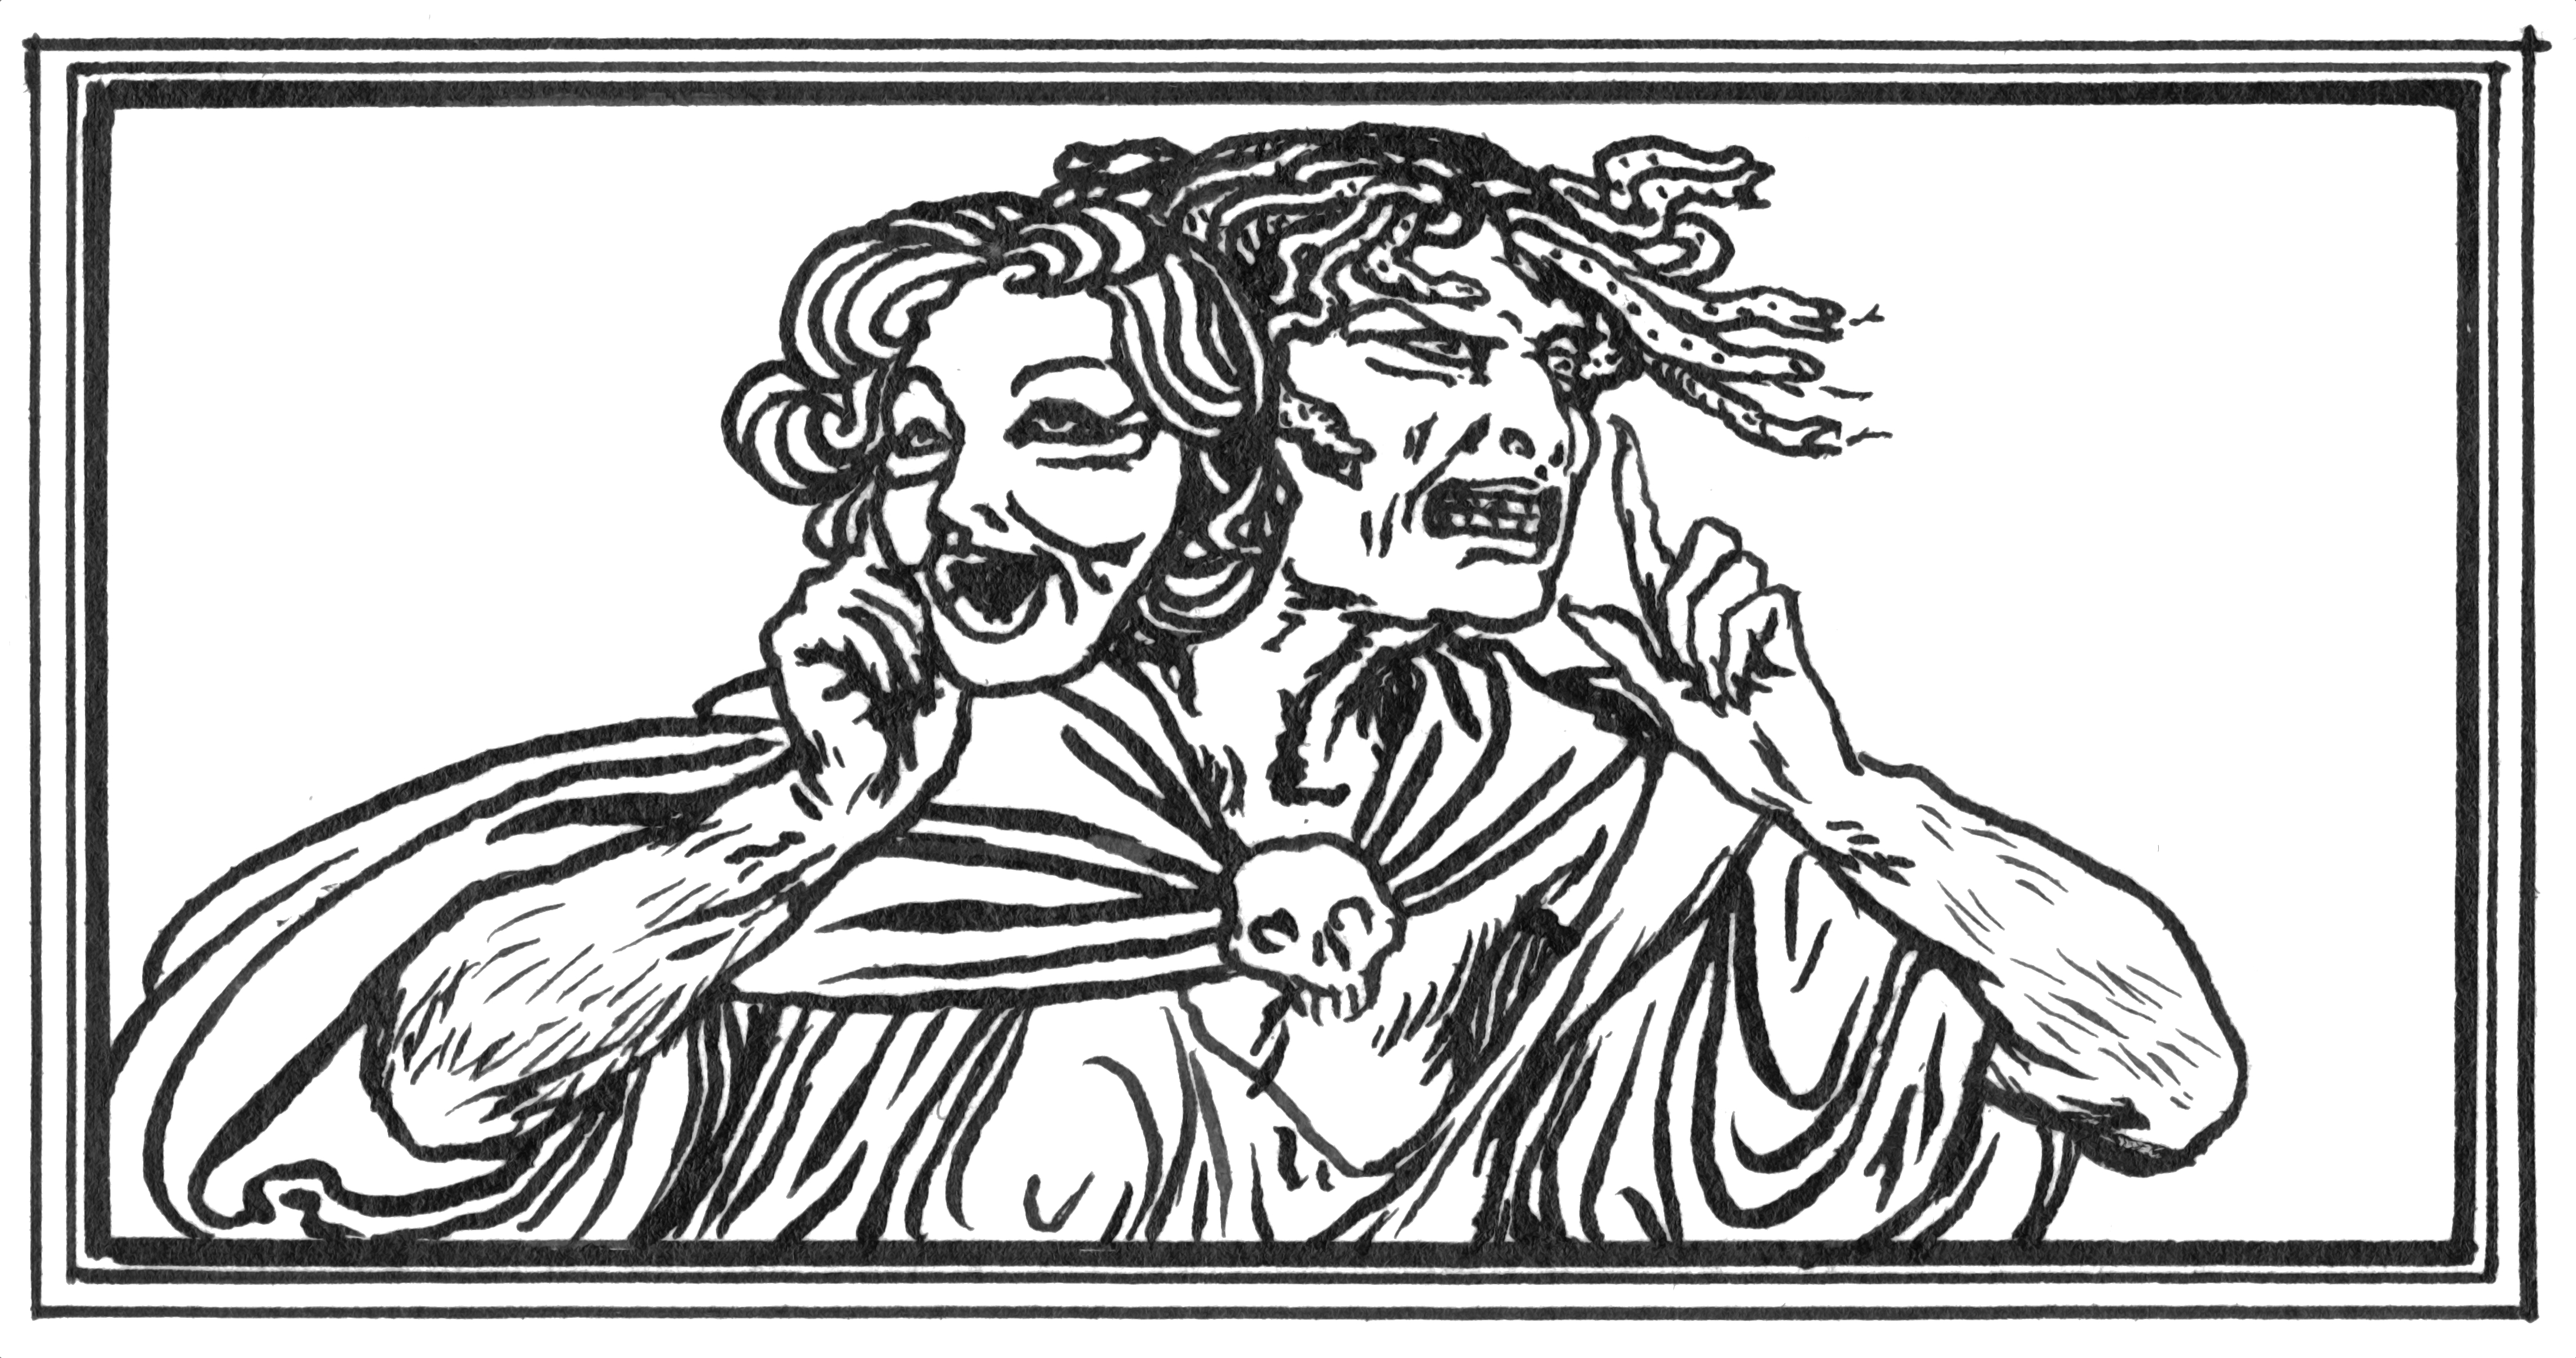
\includegraphics[width=\headerwidth]{2imasque}
\end{figure}

\verseline[Sebastian]{\hspace{\widthof{Dropping upon thy head.}}What, art thou waking?} 
\verseline[Antonio]{Do you not hear me speak?} 
\begin{verse_speech}[Sebastian] 
\hspace{\widthof{Do you not hear me speak?}}I do; and surely\\
It is a sleepy language and thou speak'st\\
Out of thy sleep. What is it thou didst say?\\
This is a strange repose, to be asleep\\
With eyes wide open; standing, speaking, moving,\\
And yet so fast asleep.
\end{verse_speech}

\begin{verse_speech}[Antonio] 
\hspace{\widthof{And yet so fast asleep.}}Noble Sebastian,\\
Thou let'st thy fortune sleep—die, rather; wink'st\\
Whiles thou art waking.
\end{verse_speech}

\begin{verse_speech}[Sebastian] 
\hspace{\widthof{Whiles thou art waking.}}Thou dost snore distinctly;\\
There's meaning in thy snores.
\end{verse_speech}

\begin{verse_speech}[Antonio] 
I am more serious than my custom: you\\
Must be so too, if heed me; which to do\\
Trebles thee o'er.
\end{verse_speech}

\verseline[Sebastian]{\hspace{\widthof{Trebles thee o'er.}}Well, I am standing water.} 
\verseline[Antonio]{I'll teach you how to flow.} 
\begin{verse_speech}[Sebastian] 
\hspace{\widthof{I'll teach you how to flow.}}Do so: to ebb\\
Hereditary sloth instructs me.
\end{verse_speech}

\begin{verse_speech}[Antonio] 
\hspace{\widthof{Hereditary sloth instructs me.}}O,\\
If you but knew how you the purpose cherish\\
Whiles thus you mock it! how, in stripping it,\\
You more invest it! Ebbing men, indeed,\\
Most often do so near the bottom run\\
By their own fear or sloth.
\end{verse_speech}

\begin{verse_speech}[Sebastian] 
\hspace{\widthof{Hereditary sloth instructs me.}}Prithee, say on:\\
The setting of thine eye and cheek proclaim\\
A matter from thee, and a birth indeed\\
Which throes thee much to yield.
\end{verse_speech}

\begin{verse_speech}[Antonio] 
\hspace{\widthof{Hereditary sloth instructs me.}}Thus, sir:\\
Although this lord of weak remembrance, this,\\
Who shall be of as little memory\\
When he is earth'd, hath here almost persuade,—\\
For he's a spirit of persuasion, only\\
Professes to persuade,—the king his son's alive,\\
'Tis as impossible that he's undrown'd\\
And he that sleeps here swims.
\end{verse_speech}

\begin{verse_speech}[Sebastian] 
\hspace{\widthof{And he that sleeps here swims.}}I have no hope\\
That he's undrown'd.
\end{verse_speech}

\begin{verse_speech}[Antonio] 
\hspace{\widthof{That he's undrown'd.}}O, out of that <no hope>\\
What great hope have you! no hope that way is\\
Another way so high a hope that even\\
Ambition cannot pierce a wink beyond,\\
But doubt discovery there. Will you grant with me\\
That Ferdinand is drown'd?
\end{verse_speech}

\verseline[Sebastian]{\hspace{\widthof{That Ferdinand is drown'd?}}He's gone.} 
\begin{verse_speech}[Antonio] 
\hspace{\widthof{That Ferdinand is drown'd? He's gone. }}Then, tell me,\\
Who's the next heir of Naples?
\end{verse_speech}

\verseline[Sebastian]{\hspace{\widthof{Who's the next heir of Naples?}}Claribel.} 

\begin{verse_speech}[Antonio] 
She that is queen of Tunis; she that dwells\\
Ten leagues beyond man's life; she that from Naples\\
Can have no note, unless the sun were post—\\
The man i' the moon's too slow—till new-born chins\\
Be rough and razorable; she that—from whom?\\
We all were sea-swallow'd, though some cast again,\\
And by that destiny to perform an act\\
Whereof what's past is prologue, what to come\\
In yours and my discharge.
\end{verse_speech}

\begin{verse_speech}[Sebastian] 
What stuff is this! how say you?\\
'Tis true, my brother's daughter's queen of Tunis;\\
So is she heir of Naples; 'twixt which regions\\
There is some space.
\end{verse_speech}

\begin{verse_speech}[Antonio] 
\hspace{\widthof{There is some space.}}A space whose every cubit\\
Seems to cry out, <How shall that Claribel\\
Measure us back to Naples? Keep in Tunis,\\
And let Sebastian wake.> Say, this were death\\
That now hath seized them; why, they were no worse\\
Than now they are. There be that can rule Naples\\
As well as he that sleeps; lords that can prate\\
As amply and unnecessarily\\
As this Gonzalo; I myself could make\\
A chough of as deep chat. O, that you bore\\
The mind that I do! what a sleep were this\\
For your advancement! Do you understand me?
\end{verse_speech}

\verseline[Sebastian]{Methinks I do.} 
\begin{verse_speech}[Antonio] 
\hspace{\widthof{Methinks I do.}}And how does your content\\
Tender your own good fortune?
\end{verse_speech}

\begin{verse_speech}[Sebastian] 
\hspace{\widthof{Tender your own good fortune?}}I remember\\
You did supplant your brother Prospero.
\end{verse_speech}

\begin{verse_speech}[Antonio] 
\hspace{\widthof{You did supplant your brother Prospero.}}True:\\
And look how well my garments sit upon me;\\
Much feater than before: my brother's servants\\
Were then my fellows; now they are my men.
\end{verse_speech}

\verseline[Sebastian]{But, for your conscience?} 
\begin{verse_speech}[Antonio] 
Ay, sir; where lies that? if 'twere a kibe,\\
'Twould put me to my slipper: but I feel not\\
This deity in my bosom: twenty consciences,\\
That stand 'twixt me and Milan, candied be they\\
And melt ere they molest! Here lies your brother,\\
No better than the earth he lies upon,\\
If he were that which now he's like, that's dead;\\
Whom I, with this obedient steel, three inches of it,\\
Can lay to bed for ever; whiles you, doing thus,\\
To the perpetual wink for aye might put\\
This ancient morsel, this Sir Prudence, who\\
Should not upbraid our course. For all the rest,\\
They'll take suggestion as a cat laps milk;\\
They'll tell the clock to any business that\\
We say befits the hour.
\end{verse_speech}

\begin{verse_speech}[Sebastian] 
\hspace{\widthof{We say befits the hour.}}Thy case, dear friend,\\
Shall be my precedent; as thou got'st Milan,\\
I'll come by Naples. Draw thy sword: one stroke\\
Shall free thee from the tribute which thou payest;\\
And I the king shall love thee.
\end{verse_speech}

\begin{verse_speech}[Antonio] 
\hspace{\widthof{And I the king shall love thee.}}Draw together;\\
And when I rear my hand, do you the like,\\
To fall it on Gonzalo.
\end{verse_speech}

\stage{They draw their swords}

\verseline[Sebastian]{\hspace{\widthof{To fall it on Gonzalo.}}O, but one word.}

\stage{They talk apart}

\stage{Re-enter \textsc{Ariel}, invisible}

\begin{verse_speech}[Ariel] 
My master through his art foresees the danger\\
That you, his friend, are in; and sends me forth—\\
For else his project dies—to keep them living.

\stage{Sings in \textsc{Gonzalo's} ear}

\begin{song}
	\songline{While you here do snoring lie,}
	\songline{Open-eyed conspiracy}
	\refrain{His time doth take.}
	\songline{If of life you keep a care,}
	\songline{Shake off slumber, and beware:}
	\refrain{Awake, awake!}
\end{song}


\end{verse_speech}

\verseline[Antonio]{(\textit{To \textsc{Sebastian}})Then let us both be sudden.} 

\begin{pictures} %Ariel wakes Alonso
	
\begin{bwbigpic}
	[\picwidth]
	{2iwake}
	{}
\end{bwbigpic}

\end{pictures}



\begin{verse_speech}[Gonzalo] 
\textit{(Waking)} Now, good angels\\
Preserve the king.\\
\end{verse_speech}

\stage{He wakes \textsc{Alonso}}

\begin{verse_speech}[Alonso] 
\textit{(To \textsc{Sebastian})} Why, how now? ho, awake! Why are you drawn?\\
Wherefore this ghastly looking?
\end{verse_speech}

\verseline[Gonzalo]{\hspace{\widthof{Wherefore this ghastly looking?}-\widthof{(To Sebastian)}}\textit{(To \textsc{Sebastian})} What's the matter?} 

\begin{verse_speech}[Sebastian] 
Whiles we stood here securing your repose,\\
Even now, we heard a hollow burst of bellowing\\
Like bulls, or rather lions: did't not wake you?\\
It struck mine ear most terribly.
\end{verse_speech}

\verseline[Alonso]{\hspace{\widthof{It struck mine ear most terribly.}}I heard nothing.} 

\begin{verse_speech}[Antonio] 
O, 'twas a din to fright a monster's ear,\\
To make an earthquake! sure, it was the roar\\
Of a whole herd of lions.
\end{verse_speech}

\verseline[Alonso]{Heard you this, Gonzalo?} 
\begin{verse_speech}[Gonzalo] 
Upon mine honour, sir, I heard a humming,\\
And that a strange one too, which did awake me:\\
I shaked you, sir, and cried: as mine eyes open'd,\\
I saw their weapons drawn: there was a noise,\\
That's verily. 'Tis best we stand upon our guard,\\
Or that we quit this place; let's draw our weapons.
\end{verse_speech}

\begin{verse_speech}[Alonso] 
Lead off this ground; and let's make further search\\
For my poor son.
\end{verse_speech}

\begin{verse_speech}[Gonzalo] 
\hspace{\widthof{For my poor son.}}Heavens keep him from these beasts!\\
For he is, sure, i' the island.
\end{verse_speech}

\verseline[Alonso]{\hspace{\widthof{For he is, sure, i' the island.}}Lead away.} 

\begin{verse_speech}[Ariel] 
Prospero my lord shall know what I have done:\\
So, king, go safely on to seek thy son.
\end{verse_speech}

\exeunt{}
\vfill
\begin{center}
\includegraphics[width=.9\textwidth]{2itailpiece}
\end{center}


\cleardoubleoddpage

\Scene{2}[Another part of the island.]

\begin{figure}[t!]
\centering
\includegraphics[width=\headerwidth]{2iiheadpiece}
\end{figure}

\enter{\textsc{Caliban} with a burden of wood. A noise of thunder heard.}

\begin{verse_speech}[Caliban] 
All the infections that the sun sucks up\\
From bogs, fens, flats, on Prosper fall and make him\\
By inch-meal a disease! His spirits hear me\\
And yet I needs must curse. But they'll nor pinch,\\
Fright me with urchin—shows, pitch me i' the mire,\\
Nor lead me, like a firebrand, in the dark\\
Out of my way, unless he bid 'em; but\\
For every trifle are they set upon me;\\
Sometime like apes that mow and chatter at me\\
And after bite me, then like hedgehogs which\\
Lie tumbling in my barefoot way and mount\\
Their pricks at my footfall; sometime am I\\
All wound with adders who with cloven tongues\\
Do hiss me into madness.

\enter{\textsc{Trinculo}}

Lo, now, lo!\\
Here comes a spirit of his, and to torment me\\
For bringing wood in slowly. I'll fall flat;\\
Perchance he will not mind me.
\end{verse_speech}

\begin{prose_speech}[Trinculo] 
Here's neither bush nor shrub, to bear off any weather at all, and another storm brewing; I hear it sing i' the wind: yond same black cloud, yond huge one, looks like a foul bombard that would shed his liquor. If it should thunder as it did before, I know not where to hide my head: yond same cloud cannot choose but fall by pailfuls. What have we here? a man or a fish? dead or alive? A fish: he smells like a fish; a very ancient and fish-like smell; a kind of not of the newest Poor-John. A strange fish! Were I in England now, as once I was, and had but this fish painted, not a holiday fool there but would give a piece of silver: there would this monster make a man; any strange beast there makes a man: when they will not give a doit to relieve a lame beggar, they will lazy out ten to see a dead Indian. Legged like a man and his fins like arms! Warm o' my troth! I do now let loose my opinion; hold it no longer: this is no fish, but an islander, that hath lately suffered by a thunderbolt.

\stage{Thunder.}

Alas, the storm is come again! my best way is to creep under his gaberdine; there is no other shelter hereabouts: misery acquaints a man with strange bed-fellows. I will here shroud till the dregs of the storm be past.
\end{prose_speech}

\begin{letter}
	\begin{figure}[tb]
		\centering
		\includegraphics[width=.5\textwidth]{2iimerfish}
	\end{figure}
\end{letter}
\begin{a4}
	\begin{figure}[tb]
		\centering
		\includegraphics[width=.4\textwidth]{2iimerfish}
	\end{figure}
\end{a4}

\enter{\textsc{Stephano}, singing: a bottle in his hand}

\begin{prose_speech}[Stephano] 
\begin{song}
	\songline{I shall no more to sea, to sea,}
	\songline{Here shall I die ashore—}
\end{song}
This is a very scurvy tune to sing at a man's funeral: well, here's my comfort. \stage{Drinks}

\stage{Sings}

\begin{song}
	\songline{The master, the swabber, the boatswain and I,}
	\songline{The gunner and his mate}
	\songline{Loved Mall, Meg and Marian and Margery,}
	\songline{But none of us cared for Kate;}
	\songline{For she had a tongue with a tang,}
	\songline{Would cry to a sailor, Go hang!}
	\songline{She loved not the savour of tar nor of pitch,}
	\songline{Yet a tailor might scratch her where'er she did itch:}
	\songline{Then to sea, boys, and let her go hang!}
\end{song}

This is a scurvy tune too: but here's my comfort.
\stage{Drinks}
\end{prose_speech}

\begin{letter}
	\begin{figure}[tb]
		\centering
		\includegraphics[width=\headerwidth]{2iifish}
	\end{figure}
\end{letter}

\begin{a4}
	\begin{figure}[tb]
		\centering
		\includegraphics[width=.7\textwidth]{2iifish}
	\end{figure}
\end{a4}

\verseline[Caliban]{Do not torment me: Oh!} 
	
\begin{prose_speech}[Stephano] What's the matter? Have we devils here? Do you put tricks upon's with savages and men of Ind, ha? I have not scaped drowning to be afeard now of your four legs; for it hath been said, As proper a man as ever went on four legs cannot make him give ground; and it shall be said so again while Stephano breathes at's nostrils.
\end{prose_speech}


\verseline[Caliban]{The spirit torments me; Oh!} 

\begin{prose_speech}[Stephano] 
This is some monster of the isle with four legs, who hath got, as I take it, an ague. Where the devil should he learn our language? I will give him some relief, if it be but for that. if I can recover him and keep him tame and get to Naples with him, he's a present for any emperor that ever trod on neat's leather.
\end{prose_speech}


\verseline[Caliban]{Do not torment me, prithee; I'll bring my wood home faster.} 

\begin{prose_speech}[Stephano] 
He's in his fit now and does not talk after the wisest. He shall taste of my bottle: if he have never drunk wine afore will go near to remove his fit. If I can recover him and keep him tame, I will not take too much for him; he shall pay for him that hath him, and that soundly.
\end{prose_speech}

\begin{prose_speech}[Caliban] 
Thou dost me yet but little hurt; thou wilt anon, I know it by thy trembling: now Prosper works upon thee.
\end{prose_speech}

\begin{prose_speech}[Stephano] 
Come on your ways; open your mouth; here is that which will give language to you, cat: open your mouth; this will shake your shaking, I can tell you, and that soundly: you cannot tell who's your friend: open your chaps again.
\end{prose_speech}

\begin{prose_speech}[Trinculo] 
I should know that voice: it should be—but he is drowned; and these are devils: O defend me!
\end{prose_speech}

\begin{prose_speech}[Stephano] 
Four legs and two voices: a most delicate monster! His forward voice now is to speak well of his friend; his backward voice is to utter foul speeches and to detract. If all the wine in my bottle will recover him, I will help his ague. Come. Amen! I will pour some in thy other mouth.
\end{prose_speech}

\verseline[Trinculo]{Stephano!}
	
\begin{prose_speech}[Stephano] 
Doth thy other mouth call me? Mercy, mercy! This is a devil, and no monster: I will leave him; I have no long spoon.
\end{prose_speech}

\begin{prose_speech}[Trinculo] 
Stephano! If thou beest Stephano, touch me and speak to me: for I am Trinculo—be not afeard—thy good friend Trinculo.
\end{prose_speech}

\begin{prose_speech}[Stephano] 
If thou beest Trinculo, come forth: I'll pull thee by the lesser legs: if any be Trinculo's legs, these are they. Thou art very Trinculo indeed! How camest thou to be the siege of this moon-calf? can he vent Trinculos?
\end{prose_speech}

\begin{prose_speech}[Trinculo] 
I took him to be killed with a thunder-stroke. But art thou not drowned, Stephano? I hope now thou art not drowned. Is the storm overblown? I hid me under the dead moon-calf's gaberdine for fear of the storm. And art thou living, Stephano? O Stephano, two Neapolitans 'scaped!
\end{prose_speech}

\verseline[Stephano]{Prithee, do not turn me about; my stomach is not constant.} 

\begin{prose_speech}[Caliban] \aside{These be fine things, an if they be not sprites. That's a brave god and bears celestial liquor. I will kneel to him.}
\end{prose_speech}

\begin{prose_speech}[Stephano] 
How didst thou 'scape? How camest thou hither? swear by this bottle how thou camest hither. I escaped upon a butt of sack which the sailors heaved o'erboard, by this bottle; which I made of the bark of a tree with mine own hands since I was cast ashore.
\end{prose_speech}

\begin{pictures} %Stephano escapes the shipwreck
	
\begin{bwbigpic}
	[\picwidth]
	{2iibarrel}
	{}
\end{bwbigpic}

\end{pictures}

\verseline[Caliban]{I'll swear upon that bottle to be thy true subject; for the liquor is not earthly.} 

\verseline[Stephano]{Here; swear then how thou escapedst.} 

\verseline[Trinculo]{Swum ashore. man, like a duck: I can swim like a duck, I'll be sworn.} 

\verseline[Stephano]{Here, kiss the book. Though thou canst swim like a duck, thou art made like a goose.} 

\verseline[Trinculo]{O Stephano. hast any more of this?} 

\verseline[Stephano]{The whole butt, man: my cellar is in a rock by the sea-side where my wine is hid. How now, moon-calf! how does thine ague?} 

\verseline[Caliban]{Hast thou not dropp'd from heaven?} 

\verseline[Stephano]{Out o' the moon, I do assure thee: I was the man i' the moon when time was.} 

\verseline[Caliban]{I have seen thee in her and I do adore thee: my mistress show'd me thee and thy dog and thy bush.} 

\verseline[Stephano]{Come, swear to that; kiss the book: I will furnish it anon with new contents swear.} 

\begin{prose_speech}[Trinculo] 
By this good light, this is a very shallow monster! I afeard of him! A very weak monster! The man i' the moon! A most poor credulous monster! Well drawn, monster, in good sooth!
\end{prose_speech}

\verseline[Caliban]{I'll show thee every fertile inch o' th' island; and I will kiss thy foot: I prithee, be my god.} 

\verseline[Trinculo]{By this light, a most perfidious and drunken monster! when 's god's asleep, he'll rob his bottle.} 

\verseline[Caliban]{I'll kiss thy foot; I'll swear myself thy subject.} 

\verseline[Stephano]{Come on then; down, and swear.} 

\verseline[Trinculo]{I shall laugh myself to death at this puppy-headed monster. A most scurvy monster! I could find in my heart to beat him,—} 

\verseline[Stephano]{Come, kiss.} 

\verseline[Trinculo]{But that the poor monster's in drink: an abominable monster!} 


\begin{pictures} %Caliban celebrates - a4
	\begin{a4}
		\begin{bwbigpic}
			[\picwidth]
			{2iinewmaster}
			{}
		\end{bwbigpic}
	\end{a4}
\end{pictures}

\begin{verse_speech}[Caliban] 
I'll show thee the best springs; I'll pluck thee berries;\\
I'll fish for thee and get thee wood enough.\\
A plague upon the tyrant that I serve!\\
I'll bear him no more sticks, but follow thee,\\
Thou wondrous man.
\end{verse_speech}

\begin{verse_speech}[Trinculo]
A most ridiculous monster, to make a wonder of a\\
Poor drunkard!
\end{verse_speech}

\begin{verse_speech}[Caliban] 
I prithee, let me bring thee where crabs grow;\\
And I with my long nails will dig thee pignuts;\\
Show thee a jay's nest and instruct thee how\\
To snare the nimble marmoset; I'll bring thee\\
To clustering filberts and sometimes I'll get thee\\
Young scamels from the rock. Wilt thou go with me?
\end{verse_speech}

\begin{prose_speech}[Stephano] 
I prithee now, lead the way without any more talking. Trinculo, the king and all our company else being drowned, we will inherit here: here; bear my bottle: fellow Trinculo, we'll fill him by and by again.
\end{prose_speech}

\begin{prose_speech}[Caliban] 
\stage{Sings drunkenly}
Farewell master; farewell, farewell!
\end{prose_speech}

\begin{pictures} %Caliban celebrates - letter
	\begin{letter}
		\begin{bwbigpic}
			[\picwidth]
			{2iinewmaster}
			{}
		\end{bwbigpic}
	\end{letter}
\end{pictures}

\verseline[Trinculo]{A howling monster: a drunken monster!} 

\begin{verse_speech}[Caliban] 
No more dams I'll make for fish\\
Nor fetch in firing\\
At requiring;\\
Nor scrape trencher, nor wash dish\\
'Ban, 'Ban, Cacaliban\\
Has a new master: get a new man.\\
Freedom, hey-day! hey-day, freedom! freedom,\\
hey-day, freedom!
\end{verse_speech}

\verseline[Stephano]{O brave monster! Lead the way.} 

\exeunt{}

\begin{letter}
	\vfill

	\begin{center}
		\includegraphics[width=.4\textwidth]{2iitailpiece}
	\end{center}
\end{letter}


\begin{a4}
	\begin{tikzpicture}[remember picture, overlay]
		\node (dropcap) at ($(current page.south)+(0cm,6cm)$) {\includegraphics[width=.3\textwidth]{2iitailpiece}};
	\end{tikzpicture}
\end{a4}






\begin{pictures}
	\cleardoubleevenpage
	\begin{letter}
	\includepdf[width=1.1\textwidth]{images/act3left.jpg}
	\includepdf[width=1.1\textwidth]{images/act3right.jpg}
	\end{letter}
	\begin{a4}
		\includepdf[width=\textwidth]{images/act3left.jpg}
		\includepdf[width=\textwidth]{images/act3right.jpg}
	\end{a4}
\end{pictures}
\begin{placeholder}
	\cleardoubleoddpage
\end{placeholder}


\Act*{3}
\Scene{1}[Before \textsc{Prospero's} Cell.]

\begin{figure}[t!]
\centering
\includegraphics[width=\headerwidth]{3iheadpiece}
\end{figure}

\enter{\textsc{Ferdinand}, bearing a log}

\begin{letter} %dropcap
	\begin{tikzpicture}[remember picture, overlay]
		\node (dropcap) at ($(current page.west)+(2.5cm,-3cm)$) {\includegraphics[width=0.125\linewidth]{3idropcapT}};
	\end{tikzpicture}
\end{letter}

\begin{a4} %dropcap
	\begin{tikzpicture}[remember picture, overlay]
		\node (dropcap) at ($(current page.west)+(2.5cm,-2.3cm)$) {\includegraphics[width=0.12\linewidth]{3idropcapT}};
	\end{tikzpicture}
\end{a4}
	
\begin{verse_speech}[Ferdinand] 
\hspace{1em}here be some sports are painful, and their labour\\
\hspace{1em}Delight in them sets off: some kinds of baseness\\
Are nobly undergone and most poor matters\\
Point to rich ends. This my mean task\\
Would be as heavy to me as odious, but\\
The mistress which I serve quickens what's dead\\
And makes my labours pleasures: O, she is\\
Ten times more gentle than her father's crabbed,\\
And he's composed of harshness. I must remove\\
Some thousands of these logs and pile them up,\\
Upon a sore injunction: my sweet mistress\\
Weeps when she sees me work, and says, such baseness\\
Had never like executor. I forget:\\
But these sweet thoughts do even refresh my labours,\\
Most busy lest, when I do it.
\end{verse_speech}

\begin{figure}[tb]
\centering
\includegraphics[width=\smallwidth]{3itail1}
\end{figure}



\enter{\textsc{Miranda}; and \textsc{Prospero} at a distance, unseen}

\begin{verse_speech}[Miranda] 
\hspace{\widthof{Most busy lest, when I do it.}}Alas, now, pray you,\\
Work not so hard: I would the lightning had\\
Burnt up those logs that you are enjoin'd to pile!\\
Pray, set it down and rest you: when this burns,\\
'Twill weep for having wearied you. My father\\
Is hard at study; pray now, rest yourself;\\
He's safe for these three hours.
\end{verse_speech}

\begin{verse_speech}[Ferdinand] 
\hspace{\widthof{He's safe for these three hours.}}O most dear mistress,\\
The sun will set before I shall discharge\\
What I must strive to do.
\end{verse_speech}

\begin{verse_speech}[Miranda] 
\hspace{\widthof{What I must strive to do.}}If you'll sit down,\\
I'll bear your logs the while: pray, give me that;\\
I'll carry it to the pile.
\end{verse_speech}

\begin{verse_speech}[Ferdinand] 
\hspace{\widthof{I'll carry it to the pile.}}No, precious creature;\\
I had rather crack my sinews, break my back,\\
Than you should such dishonour undergo,\\
While I sit lazy by.
\end{verse_speech}

\begin{verse_speech}[Miranda] 
\hspace{\widthof{While I sit lazy by.}}It would become me\\
As well as it does you: and I should do it\\
With much more ease; for my good will is to it,\\
And yours it is against.
\end{verse_speech}

\begin{verse_speech}[Prospero] 
\hspace{\widthof{And yours it is against.}}Poor worm, thou art infected!\\
This visitation shows it.
\end{verse_speech}

\verseline[Miranda]{\hspace{\widthof{This visitation shows it.}}You look wearily.}

\begin{verse_speech}[Ferdinand] 
No, noble mistress; 'tis fresh morning with me\\
When you are by at night. I do beseech you—\\
Chiefly that I might set it in my prayers—\\
What is your name?
\end{verse_speech}

\begin{verse_speech}[Miranda] 
\hspace{\widthof{What is your name?}}Miranda.—O my father,\\
I have broke your hest to say so!
\end{verse_speech}

\begin{verse_speech}[Ferdinand] 
\hspace{\widthof{I have broke your hest to say so!}}Admired Miranda!\\
Indeed the top of admiration! worth\\
What's dearest to the world! Full many a lady\\
I have eyed with best regard and many a time\\
The harmony of their tongues hath into bondage\\
Brought my too diligent ear: for several virtues\\
Have I liked several women; never any\\
With so fun soul, but some defect in her\\
Did quarrel with the noblest grace she owed\\
And put it to the foil: but you, O you,\\
So perfect and so peerless, are created\\
Of every creature's best!
\end{verse_speech}

\begin{figure}[tb]
\centering
\includegraphics[width=\smallwidth]{cupid}
\end{figure}

\begin{verse_speech}[Miranda] 
\hspace{\widthof{Of every creature's best!}}I do not know\\
One of my sex; no woman's face remember,\\
Save, from my glass, mine own; nor have I seen\\
More that I may call men than you, good friend,\\
And my dear father: how features are abroad,\\
I am skilless of; but, by my modesty,\\
The jewel in my dower, I would not wish\\
Any companion in the world but you,\\
Nor can imagination form a shape,\\
Besides yourself, to like of. But I prattle\\
Something too wildly and my father's precepts\\
I therein do forget.
\end{verse_speech}

\begin{verse_speech}[Ferdinand] 
I am in my condition\\
A prince, Miranda; I do think, a king;\\
I would, not so!—and would no more endure\\
This wooden slavery than to suffer\\
The flesh-fly blow my mouth. Hear my soul speak:\\
The very instant that I saw you, did\\
My heart fly to your service; there resides,\\
To make me slave to it; and for your sake\\
Am I this patient log-man.
\end{verse_speech}

\verseline[Miranda]{Do you love me?}

\begin{verse_speech}[Ferdinand] 
O heaven, O earth, bear witness to this sound\\
And crown what I profess with kind event\\
If I speak true! if hollowly, invert\\
What best is boded me to mischief! I\\
Beyond all limit of what else i' the world\\
Do love, prize, honour you.
\end{verse_speech}

\begin{verse_speech}[Miranda] 
I am a fool\\
To weep at what I am glad of.
\end{verse_speech}

\begin{verse_speech}[Prospero] 
Fair encounter\\
Of two most rare affections! Heavens rain grace\\
On that which breeds between 'em!
\end{verse_speech}

\verseline[Ferdinand]{Wherefore weep you?}

\begin{verse_speech}[Miranda] 
At mine unworthiness that dare not offer\\
What I desire to give, and much less take\\
What I shall die to want. But this is trifling;\\
And all the more it seeks to hide itself,\\
The bigger bulk it shows. Hence, bashful cunning!\\
And prompt me, plain and holy innocence!\\
I am your wife, it you will marry me;\\
If not, I'll die your maid: to be your fellow\\
You may deny me; but I'll be your servant,\\
Whether you will or no.
\end{verse_speech}

\begin{verse_speech}[Ferdinand] 
My mistress, dearest;\\
And I thus humble ever.
\end{verse_speech}

\verseline[Miranda]{My husband, then?}

\begin{verse_speech}[Ferdinand] 
Ay, with a heart as willing\\
As bondage e'er of freedom: here's my hand.
\end{verse_speech}

\begin{verse_speech}[Miranda] 
And mine, with my heart in't; and now farewell\\
Till half an hour hence.
\end{verse_speech}

\verseline[Ferdinand]{A thousand thousand!}

\exit{\textsc{Ferdinand} and \textsc{Miranda} severally}

\begin{verse_speech}[Prospero] 
So glad of this as they I cannot be,\\
Who are surprised withal; but my rejoicing\\
At nothing can be more. I'll to my book,\\
For yet ere supper-time must I perform\\
Much business appertaining.
\end{verse_speech}
\exit{}

\begin{figure}[b]
\centering
\includegraphics[width=\headerwidth]{3itail2}
\end{figure}

	% \begin{tikzpicture}[remember picture, overlay]
		% \node (dropcap) at ($(current page.south)+(0cm,2.5cm)$) {\includegraphics[width=.6\textwidth]{3itail2}};
	% \end{tikzpicture}
	
%!TeX root=../tempestrackham.tex

\Scene*{2}[Another part of the island.]

\begin{figure}[t]
	\centering
	\includegraphics[width=\headerwidth]{3iihead}
\end{figure}

\vspace{\textsink}

\textit{(Another part of the island.)}\centering

\enter{\textsc{Caliban}, \textsc{Stephano}, and \textsc{Trinculo}}

\verseline[Stephano]{Tell not me; when the butt is out, we will drink water; not a drop before: therefore bear up, and board 'em. Servant-monster, drink to me.}

\verseline[Trinculo]{Servant-monster! the folly of this island! They say there's but five upon this isle: we are three of them; if th' other two be brained like us, the state totters.}

\verseline[Stephano]{Drink, servant-monster, when I bid thee: thy eyes are almost set in thy head.}

\verseline[Trinculo]{Where should they be set else? he were a brave monster indeed, if they were set in his tail.}

\verseline[Stephano]{My man-monster hath drown'd his tongue in sack: for my part, the sea cannot drown me; I swam, ere I could recover the shore, five and thirty leagues off and on. By this light, thou shalt be my lieutenant, monster, or my standard.}

\verseline[Trinculo]{Your lieutenant, if you list; he's no standard.}

\verseline[Stephano]{We'll not run, Monsieur Monster.}

\verseline[Trinculo]{Nor go neither; but you'll lie like dogs and yet say nothing neither.}

\verseline[Stephano]{Moon-calf, speak once in thy life, if thou beest a good moon-calf.}

\verseline[Caliban]{How does thy honour? Let me lick thy shoe. I'll not serve him; he's not valiant.}

\verseline[Trinculo]{Thou liest, most ignorant monster: I am in case to justle a constable. Why, thou deboshed fish thou, was there ever man a coward that hath drunk so much sack as I to-day? Wilt thou tell a monstrous lie, being but half a fish and half a monster?}

\verseline[Caliban]{Lo, how he mocks me! wilt thou let him, my lord?}

\verseline[Trinculo]{<Lord> quoth he! That a monster should be such a natural!}

\verseline[Caliban]{Lo, lo, again! bite him to death, I prithee.}

\verseline[Stephano] {Trinculo, keep a good tongue in your head: if you prove a mutineer,—the next tree! The poor monster's my subject and he shall not suffer indignity.}

\verseline[Caliban]{I thank my noble lord. Wilt thou be pleased to hearken once again to the suit I made to thee?}

\verseline[Stephano]{Marry, will I. kneel and repeat it; I will stand, and so shall Trinculo.}
	
\enter{\textsc{Ariel}, invisible}

\verseline[Caliban]{As I told thee before, I am subject to a tyrant, a sorcerer, that by his cunning hath cheated me of the island.}

\verseline[Ariel]{Thou liest.}

\verseline[Caliban]{Thou liest, thou jesting monkey, thou: I would my valiant master would destroy thee! I do not lie.}

\verseline[Stephano]{Trinculo, if you trouble him any more in's tale, by this hand, I will supplant some of your teeth.}

\verseline[Trinculo]{Why, I said nothing.}

\verseline[Stephano]{Mum, then, and no more. Proceed.}

\begin{verse_speech}[Caliban] 
I say, by sorcery he got this isle;\\
From me he got it. if thy greatness will\\
Revenge it on him,—for I know thou darest,\\
But this thing dare not,—
\end{verse_speech}

\verseline[Stephano]{That's most certain.}

\verseline[Caliban]{Thou shalt be lord of it and I'll serve thee.}

\begin{verse_speech}[Stephano] How now shall this be compassed?
Canst thou bring me to the party?
\end{verse_speech}

\begin{verse_speech}[Caliban] 
Yea, yea, my lord: I'll yield him thee asleep,\\
Where thou mayst knock a nail into his bead.
\end{verse_speech}


\verseline[Ariel]{Thou liest; thou canst not.}

\begin{verse_speech}[Caliban] 
What a pied ninny's this! Thou scurvy patch!\\
I do beseech thy greatness, give him blows\\
And take his bottle from him: when that's gone\\
He shall drink nought but brine; for I'll not show him
Where the quick freshes are.
\end{verse_speech}

\verseline[Stephano]{Trinculo, run into no further danger: interrupt the monster one word further, and, by this hand, I'll turn my mercy out o' doors and make a stock-fish of thee.}

\verseline[Trinculo]{Why, what did I? I did nothing. I'll go farther off.}

\verseline[Stephano]{Didst thou not say he lied?}

\verseline[Ariel]{Thou liest.}

\begin{verse_speech}[Stephano] 
Do I so? take thou that.
	
	\stage{Beats \textsc{Trinculo}}
	
As you like this, give me the lie another time.
\end{verse_speech}



\verseline[Trinculo]{I did not give the lie. Out o' your wits and bearing too? A pox o' your bottle! this can sack and drinking do. A murrain on your monster, and the devil take your fingers!}
	
\verseline[Caliban]{Ha, ha, ha!}

\verseline[Stephano]{Now, forward with your tale. Prithee, stand farther off.}

\begin{verse_speech}[Caliban]
Beat him enough: after a little time\\
I'll beat him too.
\end{verse_speech}

\verseline[Stephano]{Stand farther. Come, proceed.}

\begin{pictures} % Sweet airs
	\begin{letter}
		\begin{colorbigpic}
			[1.1]
			{3ii_sweetairs}
			{The isle is full of\dots sounds and sweet airs, that give delight and hurt not.}
		\end{colorbigpic}
	\end{letter}
	\begin{a4}
		\begin{colorbigpic}
			[1]
			{3ii_sweetairs}
			{The isle is full of\dots sounds and sweet airs, that give delight and hurt not.}
		\end{colorbigpic}
	\end{a4}
\end{pictures}

\begin{verse_speech}[Caliban] 
Why, as I told thee, 'tis a custom with him,\\
I' th' afternoon to sleep: there thou mayst brain him,\\
Having first seized his books, or with a log\\
Batter his skull, or paunch him with a stake,\\
Or cut his wezand with thy knife. Remember\\
First to possess his books; for without them\\
He's but a sot, as I am, nor hath not\\
One spirit to command: they all do hate him\\
As rootedly as I. Burn but his books.\\
He has brave utensils,—for so he calls them—\\
Which when he has a house, he'll deck withal\\
And that most deeply to consider is\\
The beauty of his daughter; he himself\\
Calls her a nonpareil: I never saw a woman,\\
But only Sycorax my dam and she;\\
But she as far surpasseth Sycorax\\
As great'st does least.
\end{verse_speech}

\verseline[Stephano]{Is it so brave a lass?}

\begin{verse_speech}[Caliban] 
Ay, lord; she will become thy bed, I warrant.\\
And bring thee forth brave brood.
\end{verse_speech}

\verseline[Stephano] {Monster, I will kill this man: his daughter and I will be king and queen—save our graces!—and Trinculo and thyself shall be viceroys. Dost thou like the plot, Trinculo?}

\verseline[Trinculo]{Excellent.}

\begin{pictures} % Twanging
	\begin{letter}
			\begin{colorbigpic}
			[1.1]
			{3ii_twang}
			{A thousand twanging instruments}
		\end{colorbigpic}		
	\end{letter}
	\begin{a4}
			\begin{colorbigpic}
			[1]
			{3ii_twang}
			{A thousand twanging instruments}
		\end{colorbigpic}		
	\end{a4}
\end{pictures}


\verseline[Stephano]{Give me thy hand: I am sorry I beat thee; but, while thou livest, keep a good tongue in thy head.}

\begin{verse_speech}[Caliban] 
Within this half hour will he be asleep:
Wilt thou destroy him then?
\end{verse_speech}

\verseline[Stephano]{Ay, on mine honour.}

\verseline[Ariel]{This will I tell my master.}

\begin{verse_speech}[Caliban] 
Thou makest me merry; I am full of pleasure:\\
Let us be jocund: will you troll the catch\\
You taught me but while-ere?
\end{verse_speech}

\begin{verse_speech}[Stephano] At thy request, monster, I will do reason, any
reason. Come on, Trinculo, let us sing.
\stage{Sings}
\begin{song}
\songline{Flout 'em and scout 'em}
\songline{And scout 'em and flout 'em}
\songline{Thought is free.}
\end{song}
\end{verse_speech}

\verseline[Caliban]{That's not the tune.}
	
\stage{\textsc{Ariel} plays the tune on a tabour and pipe}

\verseline[Stephano]{What is this same?}

\verseline[Trinculo]{This is the tune of our catch, played by the picture of Nobody.}

\verseline[Stephano]{If thou beest a man, show thyself in thy likeness: if thou beest a devil, take't as thou list.}

\verseline[Trinculo]{O, forgive me my sins!}

\verseline[Stephano]{He that dies pays all debts: I defy thee. Mercy upon us!}

\verseline[Caliban]{Art thou afeard?}

\verseline[Stephano]{No, monster, not I.}

\begin{verse_speech}[Caliban] 
Be not afeard; the isle is full of noises,\\
Sounds and sweet airs, that give delight and hurt not.\\
Sometimes a thousand twangling instruments\\
Will hum about mine ears, and sometime voices\\
That, if I then had waked after long sleep,\\
Will make me sleep again: and then, in dreaming,\\
The clouds methought would open and show riches\\
Ready to drop upon me that, when I waked,\\
I cried to dream again.
\end{verse_speech}

\verseline[Stephano]{This will prove a brave kingdom to me, where I shall have my music for nothing.}

\begin{pictures} % Voices
	\begin{letter}
		\begin{colorbigpic}
			[1.1]
			{3ii_voices}
			{Sometime voices\dots make me sleep again}
		\end{colorbigpic}
	\end{letter}	
	\begin{a4}
		\begin{colorbigpic}
			[1]
			{3ii_voices}
			{Sometime voices\dots make me sleep again}
		\end{colorbigpic}
	\end{a4}
\end{pictures}


\verseline[Caliban]{When Prospero is destroyed.}

\verseline[Stephano]{That shall be by and by: I remember the story.}

\verseline[Trinculo]{The sound is going away; let's follow it, and after do our work.}

\verseline[Stephano]{Lead, monster; we'll follow. I would I could see this tabourer; he lays it on.}

\verseline[Trinculo]{Wilt come? I'll follow, Stephano.}
\exeunt{}




\begin{letter}
\begin{tikzpicture}[remember picture, overlay]
	\node (img) at ($(current page.south)+(0cm,6cm)$) {\includegraphics[width=.6\textwidth]{lutemermaid}};
\end{tikzpicture}
\end{letter}


%!TeX root=../tempestrackham.tex
\Scene*{3}[Another part of the island.]


\begin{figure}[t]
	\centering
	\includegraphics[width=\headerwidth]{3iiihead}
\end{figure}

\vspace{\textsink}
\textit{(Another part of the island.)}\centering


\enter{\textsc{Alonso}, \textsc{Sebastian}, \textsc{Antonio}, \textsc{Gonzalo}, \textsc{Adrian}, \textsc{Francisco}, and others}

\begin{verse_speech}[Gonzalo] 
By'r lakin, I can go no further, sir;\\
My old bones ache: here's a maze trod indeed\\
Through forth-rights and meanders! By your patience,\\
I needs must rest me.
\end{verse_speech}

\begin{verse_speech}[Alonso] 
\hspace{\widthof{I needs must rest me.}}Old lord, I cannot blame thee,\\
Who am myself attach'd with weariness,\\
To the dulling of my spirits: sit down, and rest.\\
Even here I will put off my hope and keep it\\
No longer for my flatterer: he is drown'd\\
Whom thus we stray to find, and the sea mocks\\
Our frustrate search on land. Well, let him go.
\end{verse_speech}

\begin{verse_speech}[Antonio] 
\asideto{Sebastian}{I am right glad that he's so out of hope.\\
Do not, for one repulse, forego the purpose\\
That you resolved to effect.}
\end{verse_speech}

\begin{verse_speech}[Sebastian] 
\asideto{Antonio}{\hspace{\widthof{That you resolved to effect.}-\widthof{[Aside to Antonio]}}The next advantage\\
Will we take throughly.}
\end{verse_speech}

\begin{verse_speech}[Antonio] 
\asideto{Sebastian}{
\hspace{\widthof{Will we take throughly.}-\widthof{[Aside to Sebastian]}}Let it be to-night;\\
For, now they are oppress'd with travel, they\\
Will not, nor cannot, use such vigilance\\
As when they are fresh.}
\end{verse_speech}

\verseline[Sebastian]{\asideto{Antonio}{\hspace{\widthof{As when they are fresh.}-\widthof{[Aside to Antonio]}}I say, to-night: no more.}}

\stage{Solemn and strange music}

\verseline[Alonso]{What harmony is this? My good friends, hark!}

\verseline[Gonzalo]{Marvellous sweet music!}

\enter{\textsc{Prospero} above, invisible. Enter several strange Shapes, bringing in a banquet; they dance about it with gentle actions of salutation; and, inviting the King, \&c. to eat, they depart}

\verseline[Alonso]{Give us kind keepers, heavens! What were these?}


\begin{pictures} % banquet
	\begin{letter}
		\begin{colorbigpic}
			[1.1]
			{3iii_banquet}
			{\textit{Enter several strange Shapes, bringing in a banquet}}
		\end{colorbigpic}
	\end{letter}
	\begin{a4}
		\begin{colorbigpic}
			[1]
			{3iii_banquet}
			{\textit{Enter several strange Shapes, bringing in a banquet}}
		\end{colorbigpic}
	\end{a4}
\end{pictures}

\begin{verse_speech}[Sebastian] 
A living drollery. Now I will believe\\
That there are unicorns, that in Arabia\\
There is one tree, the phoenix' throne, one phoenix\\
At this hour reigning there.
\end{verse_speech}

\begin{verse_speech}[Antonio] 
\hspace{\widthof{At this hour reigning there.}}I'll believe both;\\
And what does else want credit, come to me,\\
And I'll be sworn 'tis true: travellers ne'er did lie,\\
Though fools at home condemn 'em.
\end{verse_speech}

\begin{verse_speech}[Gonzalo] 
\hspace{\widthof{Though fools at home condemn 'em.}}If in Naples\\
I should report this now, would they believe me?\\
If I should say, I saw such islanders—\\
For, certes, these are people of the island—\\
Who, though they are of monstrous shape, yet, note,\\
Their manners are more gentle-kind than of\\
Our human generation you shall find\\
Many, nay, almost any.
\end{verse_speech}


\begin{verse_speech}[Prospero]
\aside{\hspace{\widthof{Many, nay, almost any.}-\widthof{[Aside]}}Honest lord,\\
Thou hast said well; for some of you there present\\
Are worse than devils.}
\end{verse_speech}


\begin{verse_speech}[Alonso] 
\hspace{\widthof{Are worse than devils.}}I cannot too much muse\\
Such shapes, such gesture and such sound, expressing,\\
Although they want the use of tongue, a kind\\
Of excellent dumb discourse.
\end{verse_speech}

\verseline[Prospero]{\aside{\hspace{\widthof{Of excellent dumb discourse.}-\widthof{[Aside]}}Praise in departing.}}

\verseline[Francisco]{They vanish'd strangely.}

\begin{verse_speech}[Sebastian] 
No matter, since\\
They have left their viands behind; for we have stomachs.\\
Will't please you taste of what is here?
\end{verse_speech}

\verseline[Alonso]{\hspace{\widthof{Will't please you taste of what is here?}}Not I.}

\begin{verse_speech}[Gonzalo] 
Faith, sir, you need not fear. When we were boys,\\
Who would believe that there were mountaineers\\
Dew-lapp'd like bulls, whose throats had hanging at 'em\\
Wallets of flesh? or that there were such men\\
Whose heads stood in their breasts? which now we find\\
Each putter-out of five for one will bring us\\
Good warrant of.
\end{verse_speech}

\begin{verse_speech}[Alonso] 
\hspace{\widthof{Good warrant of.}}I will stand to and feed,\\
Although my last: no matter, since I feel\\
The best is past. Brother, my lord the duke,\\
Stand to and do as we.
\end{verse_speech}


\stage{Thunder and lightning. Enter \textsc{Ariel}, like a harpy; claps his wings upon the table; and, with a quaint device, the banquet vanishes}

\begin{verse_speech}[Ariel] 
You are three men of sin, whom Destiny,\\
That hath to instrument this lower world\\
And what is in't, the never-surfeited sea\\
Hath caused to belch up you; and on this island\\
Where man doth not inhabit; you 'mongst men\\
Being most unfit to live. I have made you mad;\\
And even with such-like valour men hang and drown\\
Their proper selves.

\stage{\textsc{Alonso}, \textsc{Sebastian} \&c. draw their swords}

\hspace{\widthof{Their proper selves.}}You fools! I and my fellows\\
Are ministers of Fate: the elements,\\
Of whom your swords are temper'd, may as well\\
Wound the loud winds, or with bemock'd-at stabs\\
Kill the still-closing waters, as diminish\\
One dowle that's in my plume: my fellow-ministers\\
Are like invulnerable. If you could hurt,\\
Your swords are now too massy for your strengths\\
And will not be uplifted. But remember—\\
For that's my business to you—that you three\\
From Milan did supplant good Prospero;\\
Exposed unto the sea, which hath requit it,\\
Him and his innocent child: for which foul deed\\
The powers, delaying, not forgetting, have\\
Incensed the seas and shores, yea, all the creatures,\\
Against your peace. Thee of thy son, Alonso,\\
They have bereft; and do pronounce by me:\\
Lingering perdition, worse than any death\\
Can be at once, shall step by step attend\\
You and your ways; whose wraths to guard you from—\\
Which here, in this most desolate isle, else falls\\
Upon your heads—is nothing but heart-sorrow\\
And a clear life ensuing.
\end{verse_speech}


\stage{He vanishes in thunder; then, to soft music, enter the Shapes again, and dance, with mocks and mows, and carrying out the table}

\begin{verse_speech}[Prospero] 
Bravely the figure of this harpy hast thou\\
Perform'd, my Ariel; a grace it had, devouring:\\
Of my instruction hast thou nothing bated\\
In what thou hadst to say: so, with good life\\
And observation strange, my meaner ministers\\
Their several kinds have done. My high charms work\\
And these mine enemies are all knit up\\
In their distractions; they now are in my power;\\
And in these fits I leave them, while I visit\\
Young Ferdinand, whom they suppose is drown'd,\\
And his and mine loved darling.
\end{verse_speech}

\stage{He exits, above.}

\begin{verse_speech}[Gonzalo] 
I' the name of something holy, sir, why stand you\\
In this strange stare?
\end{verse_speech}

\begin{verse_speech}[Alonso] 
\hspace{\widthof{In this strange stare?}}O, it is monstrous, monstrous:\\
Methought the billows spoke and told me of it;\\
The winds did sing it to me, and the thunder,\\
That deep and dreadful organ-pipe, pronounced\\
The name of Prosper: it did bass my trespass.\\
Therefore my son i' the ooze is bedded, and\\
I'll seek him deeper than e'er plummet sounded\\
And with him there lie mudded.
\end{verse_speech}

\exit{Alonso}

\begin{verse_speech}[Sebastian] 
But one fiend at a time,\\
I'll fight their legions o'er.
\end{verse_speech}

\verseline[Antonio]{\hspace{\widthof{I'll fight their legions o'er.}}I'll be thy second.}

\exit{\textsc{Sebastian} and \textsc{Antonio}}

\begin{verse_speech}[Gonzalo] 
All three of them are desperate: their great guilt,\\
Like poison given to work a great time after,\\
Now 'gins to bite the spirits. I do beseech you\\
That are of suppler joints, follow them swiftly\\
And hinder them from what this ecstasy\\
May now provoke them to.
\end{verse_speech}

\verseline[Adrian]{\hspace{\widthof{May now provoke them to.}}Follow, I pray you.}

\exeunt{}

\begin{letter}
	\begin{tikzpicture}[remember picture, overlay]
		\node (img) at ($(current page.south)+(0cm,7cm)$) {\includegraphics[width=.3\textwidth]{harpy}};
	\end{tikzpicture}
\end{letter}

\begin{a4}
	\begin{tikzpicture}[remember picture, overlay]
		\node (img) at ($(current page.south)+(0cm,4cm)$) {\includegraphics[width=.3\textwidth]{harpy}};
	\end{tikzpicture}
\end{a4}


\begin{pictures}
	\cleardoubleevenpage
	\begin{letter}
		\includepdf[width=1.1\textwidth]{images/act4left.jpg}
		\includepdf[width=1.1\textwidth]{images/act4right.jpg}
	\end{letter}
	\begin{a4}
		\includepdf[width=\textwidth]{images/act4left.jpg}
		\includepdf[width=\textwidth]{images/act4right.jpg}
	\end{a4}
\end{pictures}
\begin{placeholder}
	\cleardoubleoddpage
\end{placeholder}

%!TeX root=../tempestrackham.tex

\Act*{4}
\Scene*{1}[Before \textsc{Prospero's} cell.]

\begin{figure}[t]
	\centering
	\includegraphics[width=\headerwidth]{4ihead}
\end{figure}

\vspace{\textsink}

\textit{(Before \textsc{Prospero's} cell.)}\centering


\enter{\textsc{Prospero}, \textsc{Ferdinand}, and \textsc{Miranda}}

\begin{verse_speech}[Prospero] 
If I have too austerely punish'd you,\\
Your compensation makes amends, for I\\
Have given you here a third of mine own life,\\
Or that for which I live; who once again\\
I tender to thy hand: all thy vexations\\
Were but my trials of thy love and thou\\
Hast strangely stood the test here, afore Heaven,\\
I ratify this my rich gift. O Ferdinand,\\
Do not smile at me that I boast her off,\\
For thou shalt find she will outstrip all praise\\
And make it halt behind her.
\end{verse_speech}

\begin{pictures} % Rabble
	\begin{letter}
		\begin{colorbigpic}
			[1.1]
			{4i_rabble}
			{Go bring the rabble\dots here to this place}
		\end{colorbigpic}
	\end{letter}
	\begin{a4}
		\begin{colorbigpic}
			[1]
			{4i_rabble}
			{Go bring the rabble\dots here to this place}
		\end{colorbigpic}
	\end{a4}
\end{pictures}


\begin{verse_speech}[Ferdinand] 
\hspace{\widthof{And make it halt behind her.}}I do believe it\\
Against an oracle.
\end{verse_speech}

\begin{verse_speech}[Prospero] 
Then, as my gift and thine own acquisition\\
Worthily purchased take my daughter: but\\
If thou dost break her virgin-knot before\\
All sanctimonious ceremonies may\\
With full and holy rite be minister'd,\\
No sweet aspersion shall the heavens let fall\\
To make this contract grow: but barren hate,\\
Sour-eyed disdain and discord shall bestrew\\
The union of your bed with weeds so loathly\\
That you shall hate it both: therefore take heed,\\
As Hymen's lamps shall light you.
\end{verse_speech}

\begin{verse_speech}[Ferdinand] 
\hspace{\widthof{As Hymen's lamps shall light you.}}As I hope\\
For quiet days, fair issue and long life,\\
With such love as 'tis now, the murkiest den,\\
The most opportune place, the strong'st suggestion.\\
Our worser genius can, shall never melt\\
Mine honour into lust, to take away\\
The edge of that day's celebration\\
When I shall think: or Phoebus' steeds are founder'd,\\
Or Night kept chain'd below.
\end{verse_speech}

\begin{verse_speech}[Prospero] 
\hspace{\widthof{Or Night kept chain'd below.}}Fairly spoke.\\
Sit then and talk with her; she is thine own.\\
What, Ariel! my industrious servant, Ariel!
\end{verse_speech}



\begin{pictures} % Tripping
	\begin{letter}
		\begin{colorbigpic}
			[1.1]
			{4i_tripping}
			{Each one, tripping on his toe}
		\end{colorbigpic}
	\end{letter}
	\begin{a4}
		\begin{colorbigpic}
			[1.1]
			{4i_tripping}
			{Each one, tripping on his toe}
		\end{colorbigpic}
	\end{a4}
\end{pictures}

\enter{\textsc{Ariel}}

\verseline[Ariel]{What would my potent master? here I am.}

\begin{verse_speech}[Prospero] 
Thou and thy meaner fellows your last service\\
Did worthily perform; and I must use you\\
In such another trick. Go bring the rabble,\\
O'er whom I give thee power, here to this place:\\
Incite them to quick motion; for I must\\
Bestow upon the eyes of this young couple\\
Some vanity of mine art: it is my promise,\\
And they expect it from me.
\end{verse_speech}

\verseline[Ariel]{\hspace{\widthof{And they expect it from me.}}Presently?}

\verseline[Prospero]{Ay, with a twink.}

\begin{verse_speech}[Ariel] 
	\begin{song}
\songline{Before you can say <come> and <go,>}
\songline{And breathe twice and cry <so, so,>}
\songline{Each one, tripping on his toe,}
\songline{Will be here with mop and mow.}
\songline{Do you love me, master? no?}
\end{song}
\end{verse_speech}

\begin{verse_speech}[Prospero] 
Dearly my delicate Ariel. Do not approach\\
Till thou dost hear me call.
\end{verse_speech}

\verseline[Ariel]{\hspace{\widthof{Till thou dost hear me call.}}Well, I conceive.}
\begin{letter}
	\enlargethispage{\baselineskip}
\end{letter}
\stage{He exits.}



\begin{pictures} % Enter Iris
	\begin{letter}
		\begin{colorbigpic}
			[1.1]
			{4i_iris}
			{\textit{Soft music. Enter Iris.}}
		\end{colorbigpic}
	\end{letter}
	\begin{a4}
		\begin{colorbigpic}
			[1]
			{4i_iris}
			{\textit{Soft music. Enter Iris.}}
		\end{colorbigpic}
	\end{a4}
\end{pictures}

\begin{verse_speech}[Prospero] 
Look thou be true; do not give dalliance\\
Too much the rein: the strongest oaths are straw\\
To the fire i' the blood: be more abstemious,\\
Or else, good night your vow!
\end{verse_speech}

\begin{verse_speech}[Ferdinand] 
\hspace{\widthof{Or else, good night your vow!}}I warrant you, sir;\\
The white cold virgin snow upon my heart\\
Abates the ardour of my liver.
\end{verse_speech}

\begin{verse_speech}[Prospero] 
\hspace{\widthof{Abates the ardour of my liver.}}Well.\\
Now come, my Ariel! bring a corollary,\\
Rather than want a spirit: appear and pertly!\\
No tongue! all eyes! be silent.
\end{verse_speech}

\stage{Soft music. Enter \textsc{Iris}.}

\begin{letter}
	\begin{figure}[tb]
		\centering
		\includegraphics[width=0.3\textwidth]{singingfairies}
	\end{figure}
\end{letter}

\begin{verse_speech}[Iris] 
Ceres, most bounteous lady, thy rich leas\\
Of wheat, rye, barley, vetches, oats and pease;\\
Thy turfy mountains, where live nibbling sheep,\\
And flat meads thatch'd with stover, them to keep;\\
Thy banks with pioned and twilled brims,\\
Which spongy April at thy hest betrims,\\
To make cold nymphs chaste crowns; and thy broom-groves,\\
Whose shadow the dismissed bachelor loves,\\
Being lass-lorn: thy pole-clipt vineyard;\\
And thy sea-marge, sterile and rocky-hard,\\
Where thou thyself dost air;—the queen o' the sky,\\
Whose watery arch and messenger am I,\\
Bids thee leave these, and with her sovereign grace,\\
Here on this grass-plot, in this very place,\\
To come and sport: her peacocks fly amain:\\
Approach, rich Ceres, her to entertain.
\end{verse_speech}

\enter{\textsc{Ceres}}

\begin{verse_speech}[Ceres] 
Hail, many-colour'd messenger, that ne'er\\
Dost disobey the wife of Jupiter;\\
Who with thy saffron wings upon my flowers\\
Diffusest honey-drops, refreshing showers,\\
And with each end of thy blue bow dost crown\\
My bosky acres and my unshrubb'd down,\\
Rich scarf to my proud earth; why hath thy queen\\
Summon'd me hither, to this short-grass'd green?
\end{verse_speech}


\begin{verse_speech}[Iris] 
A contract of true love to celebrate;\\
And some donation freely to estate\\
On the blest lovers.
\end{verse_speech}

\begin{verse_speech}[Ceres] 
\hspace{\widthof{On the blest lovers.}}Tell me, heavenly bow,\\
If Venus or her son, as thou dost know,\\
Do now attend the queen? Since they did plot\\
The means that dusky Dis my daughter got,\\
Her and her blind boy's scandal'd company\\
I have forsworn.
\end{verse_speech}


\begin{pictures} % Temperate
	\begin{letter}
		\begin{colorbigpic}
			[1.1]
			{4i_temperate}
			{Come, temperate nymphs}
		\end{colorbigpic}
	\end{letter}
	\begin{a4}
		\begin{colorbigpic}
			[1]
			{4i_temperate}
			{Come, temperate nymphs}
		\end{colorbigpic}
	\end{a4}
\end{pictures}


\begin{verse_speech}[Iris] 
\hspace{\widthof{I have forsworn.}}Of her society\\
Be not afraid: I met her deity\\
Cutting the clouds towards Paphos and her son\\
Dove-drawn with her. Here thought they to have done\\
Some wanton charm upon this man and maid,\\
Whose vows are, that no bed-right shall be paid\\
Till Hymen's torch be lighted: but vain;\\
Mars's hot minion is returned again;\\
Her waspish-headed son has broke his arrows,\\
Swears he will shoot no more but play with sparrows\\
And be a boy right out.
\end{verse_speech}


\begin{verse_speech}[Ceres] 
\hspace{\widthof{And be a boy right out.}}High'st queen of state,\\
Great Juno, comes; I know her by her gait.
\end{verse_speech}

\enter{\textsc{Juno}}

\begin{verse_speech}[Juno] 
How does my bounteous sister? Go with me\\
To bless this twain, that they may prosperous be\\
And honour'd in their issue.
\end{verse_speech}

\stage{They sing:}

\begin{verse_speech}[Juno]
	\begin{song}
\songline{Honour, riches, marriage-blessing,}
\songline{Long continuance, and increasing,}
\songline{Hourly joys be still upon you!}
\songline{Juno sings her blessings upon you.}
\end{song}
\end{verse_speech}

\begin{verse_speech}[Ceres] 
	\begin{song}
\songline{Earth's increase, foison plenty,}
\songline{Barns and garners never empty,}
\songline{Vines and clustering bunches growing,}
\songline{Plants with goodly burthen bowing;}
\songline{Spring come to you at the farthest}
\songline{In the very end of harvest!}
\songline{Scarcity and want shall shun you;}
\songline{Ceres' blessing so is on you.}
\end{song}
\end{verse_speech}






\begin{verse_speech}[Ferdinand] 
This is a most majestic vision, and\\
Harmoniously charmingly. May I be bold\\
To think these spirits?
\end{verse_speech}


\begin{verse_speech}[Prospero] 
\hspace{\widthof{To think these spirits?}}Spirits, which by mine art\\
I have from their confines call'd to enact\\
My present fancies.
\end{verse_speech}

\begin{verse_speech}[Ferdinand] 
\hspace{\widthof{My present fancies.}}Let me live here ever;\\
So rare a wonder'd father and a wife\\
Makes this place Paradise.
\end{verse_speech}

\stage{\textsc{Juno} and \textsc{Ceres} whisper, and send \textsc{Iris} on employment.}

\begin{verse_speech}[Prospero] 
\hspace{\widthof{Makes this place Paradise.}}Sweet, now, silence!\\
Juno and Ceres whisper seriously;\\
There's something else to do: hush, and be mute,\\
Or else our spell is marr'd.
\end{verse_speech}

\begin{verse_speech}[Iris] 
You nymphs, call'd Naiads, of the windring brooks,\\
With your sedged crowns and ever-harmless looks,\\
Leave your crisp channels and on this green land\\
Answer your summons; Juno does command:\\
Come, temperate nymphs, and help to celebrate\\
A contract of true love; be not too late.\\
\enter{certain Nymphs}
You sunburnt sicklemen, of August weary,\\
Come hither from the furrow and be merry:\\
Make holiday; your rye-straw hats put on\\
And these fresh nymphs encounter every one\\
In country footing.
\end{verse_speech}

\enter{certain Reapers, properly habited: they join with the Nymphs in a graceful dance; towards the end whereof \textsc{Prospero} starts suddenly, and speaks; after which, to a strange, hollow, and confused noise, they heavily vanish}

\begin{verse_speech}[Prospero] 
	\aside{I had forgot that foul conspiracy\\
Of the beast Caliban and his confederates\\
Against my life: the minute of their plot\\
Is almost come.}
\stage{To the Spirits}
Well done! avoid; no more!
\end{verse_speech}

\begin{verse_speech}[Ferdinand] 
This is strange: your father's in some passion\\
That works him strongly.
\end{verse_speech}

\begin{verse_speech}[Miranda] 
\hspace{\widthof{That works him strongly.}}Never till this day\\
Saw I him touch'd with anger so distemper'd.
\end{verse_speech}

\begin{verse_speech}[Prospero] 
You do look, my son, in a moved sort,\\
As if you were dismay'd: be cheerful, sir.\\
Our revels now are ended. These our actors,\\
As I foretold you, were all spirits and\\
Are melted into air, into thin air:\\
And, like the baseless fabric of this vision,\\
The cloud-capp'd towers, the gorgeous palaces,\\
The solemn temples, the great globe itself,\\
Ye all which it inherit, shall dissolve\\
And, like this insubstantial pageant faded,\\
Leave not a rack behind. We are such stuff\\
As dreams are made on, and our little life\\
Is rounded with a sleep. Sir, I am vex'd;\\
Bear with my weakness; my, brain is troubled:\\
Be not disturb'd with my infirmity:\\
If you be pleased, retire into my cell\\
And there repose: a turn or two I'll walk,\\
To still my beating mind.
\end{verse_speech}

\verseline[Ferdinand]{\textit{[With Miranda]}\hspace{\widthof{To still my beating mind.}-\widthof{[With Miranda]}} We wish your peace.}

\exeunt{}

\verseline[Prospero]{Come with a thought I thank thee, Ariel: come.}
\enter{\textsc{Ariel}}

\verseline[Ariel]{Thy thoughts I cleave to. What's thy pleasure?}


\begin{verse_speech}[Prospero] 
\hspace{\widthof{Thy thoughts I cleave to. What's thy pleasure?}}Spirit,\\
We must prepare to meet with Caliban.
\end{verse_speech}

\begin{pictures} % Reapers properly habited 
	\begin{letter}
		\begin{colorbigpic}
			[1.1]
			{4i_habited}
			{\textit{Enter certain Reapers, properly habited}}
		\end{colorbigpic}
	\end{letter}
	\begin{a4}
		\begin{colorbigpic}
			[1.1]
			{4i_habited}
			{\textit{Enter certain Reapers, properly habited}}
		\end{colorbigpic}
	\end{a4}
\end{pictures}


\begin{verse_speech}[Ariel] 
Ay, my commander: when I presented Ceres,\\
I thought to have told thee of it, but I fear'd\\
Lest I might anger thee.
\end{verse_speech}

\verseline[Prospero]{Say again, where didst thou leave these varlets?}



\begin{verse_speech}[Ariel] 
I told you, sir, they were red-hot with drinking;\\
So fun of valour that they smote the air\\
For breathing in their faces; beat the ground\\
For kissing of their feet; yet always bending\\
Towards their project. Then I beat my tabour;\\
At which, like unback'd colts, they prick'd their ears,\\
Advanced their eyelids, lifted up their noses\\
As they smelt music: so I charm'd their ears\\
That calf-like they my lowing follow'd through\\
Tooth'd briers, sharp furzes, pricking goss and thorns,\\
Which entered their frail shins: at last I left them\\
I' the filthy-mantled pool beyond your cell,\\
There dancing up to the chins, that the foul lake\\
O'erstunk their feet.
\end{verse_speech}

\begin{verse_speech}[Prospero] 
\hspace{\widthof{O'erstunk their feet.}}This was well done, my bird.\\
Thy shape invisible retain thou still:\\
The trumpery in my house, go bring it hither,\\
For stale to catch these thieves.
\end{verse_speech}

\verseline[Ariel]{\hspace{\widthof{For stale to catch these thieves.}}I go, I go.}

\exit{Ariel}

\begin{verse_speech}[Prospero] 
A devil, a born devil, on whose nature\\
Nurture can never stick; on whom my pains,\\
Humanely taken, all, all lost, quite lost;\\
And as with age his body uglier grows,\\
So his mind cankers. I will plague them all,\\
Even to roaring.

\stage{Re-enter \textsc{Ariel}, loaden with glistering apparel, \&c}

Come, hang them on this line.

\end{verse_speech}

\stage{\textsc{Prospero} and \textsc{Ariel} remain invisible. Enter \textsc{Caliban}, \textsc{Stephano}, and \textsc{Trinculo}, all wet}

\begin{verse_speech}[Caliban] 
Pray you, tread softly, that the blind mole may not\\
Hear a foot fall: we now are near his cell.
\end{verse_speech}

\verseline[Stephano]{Monster, your fairy, which you say is a harmless fairy, has done little better than played the Jack with us.}

\verseline[Trinculo]{Monster, I do smell all horse-piss; at which my nose is in great indignation.}

\verseline[Stephano]{So is mine. Do you hear, monster? If I should take a displeasure against you, look you,—}

\verseline[Trinculo]{Thou wert but a lost monster.}

\begin{verse_speech}[Caliban] 
Good my lord, give me thy favour still.\\
Be patient, for the prize I'll bring thee to\\
Shall hoodwink this mischance: therefore speak softly.\\
All's hush'd as midnight yet.
\end{verse_speech}

\verseline[Trinculo]{Ay, but to lose our bottles in the pool,—}

\verseline[Stephano]{There is not only disgrace and dishonour in that, monster, but an infinite loss.}

\verseline[Trinculo]{That's more to me than my wetting: yet this is your harmless fairy, monster.}

\verseline[Stephano]{I will fetch off my bottle, though I be o'er ears for my labour.}

\begin{verse_speech}[Caliban] 
Prithee, my king, be quiet. Seest thou here,\\
This is the mouth o' the cell: no noise, and enter.\\
Do that good mischief which may make this island\\
Thine own for ever, and I, thy Caliban,\\
For aye thy foot-licker.
\end{verse_speech}

\verseline[Stephano]{Give me thy hand. I do begin to have bloody thoughts.}

\verseline[Trinculo]{\textit{(Seeing the apparel)} O king Stephano! O peer! O worthy Stephano! look what a wardrobe here is for thee!}

\verseline[Caliban]{Let it alone, thou fool; it is but trash.}

\begin{prose_speech}[Trinculo]
O, ho, monster! we know what belongs to a frippery.
\stage{He puts on one of the gowns.}
O king Stephano!
\end{prose_speech}

\verseline[Stephano]{Put off that gown, Trinculo; by this hand, I'll have that gown.}

\verseline[Trinculo]{Thy grace shall have it.}

\begin{verse_speech}[Caliban] 
The dropsy drown this fool! What do you mean\\
To dote thus on such luggage? Let's alone\\
And do the murder first: if he awake,\\
From toe to crown he'll fill our skins with pinches,\\
Make us strange stuff.
\end{verse_speech}

\begin{prose_speech}[Stephano]
Be you quiet, monster. Mistress line, is not this my jerkin? 

\stage{He takes a jacket from the tree.}

Now is the jerkin under the line: now, jerkin, you are like to lose your hair and prove a bald jerkin.
\end{prose_speech}


\verseline[Trinculo]{Do, do: we steal by line and level, an't like your grace.}

\verseline[Stephano]{I thank thee for that jest; here's a garment for't: wit shall not go unrewarded while I am king of this country. <Steal by line and level> is an excellent pass of pate; there's another garment for't.}

\verseline[Trinculo]{Monster, come, put some lime upon your fingers, and away with the rest.}
	
\begin{verse_speech}[Caliban] 
I will have none on't: we shall lose our time,\\
And all be turn'd to barnacles, or to apes\\
With foreheads villanous low.
\end{verse_speech}

\verseline[Stephano]{Monster, lay-to your fingers: help to bear this away where my hogshead of wine is, or I'll turn you out of my kingdom: go to, carry this.}

\verseline[Trinculo]{And this.}

\verseline[Stephano]{Ay, and this.}

\stage{A noise of hunters heard. Enter divers Spirits, in shape of dogs and hounds, and hunt them about, \textsc{Prospero} and \textsc{Ariel} setting them on.}

\verseline[Prospero]{Hey, Mountain, hey!}

\verseline[Ariel]{Silver I there it goes, Silver!}

\begin{verse_speech}[Prospero] 
Fury, Fury! there, Tyrant, there! hark! hark!
	
\stage{\textsc{Caliban}, \textsc{Stephano}, and \textsc{Trinculo} are driven off}

Go charge my goblins that they grind their joints\\
With dry convulsions, shorten up their sinews\\
With agèd cramps, and more pinch-spotted make them\\
Than pard or cat o' mountain.
\end{verse_speech}

\verseline[Ariel]{\hspace{\widthof{Than pard or cat o' mountain.}}Hark, they roar!}

\begin{pictures} % Goblins
	\begin{letter}
		\begin{colorbigpic}
			[1.1]
			{4i_goblins}
			{Go charge my goblins that they grind their joints with dry convulsions}
		\end{colorbigpic}
	\end{letter}
	\begin{a4}
		\begin{colorbigpic}
			[1.1]
			{4i_goblins}
			{Go charge my goblins that they grind their joints with dry convulsions}
		\end{colorbigpic}
	\end{a4}
\end{pictures}

\begin{verse_speech}[Prospero] 
Let them be hunted soundly. At this hour\\
Lie at my mercy all mine enemies:\\
Shortly shall all my labours end, and thou\\
Shalt have the air at freedom: for a little\\
Follow, and do me service.
\end{verse_speech}

\exeunt{}

\begin{letter}
	\begin{figure}[b]
		\centering
		\includegraphics[width=\textwidth]{merheader}
	\end{figure}
\end{letter}

\begin{a4}
	\begin{tikzpicture}[remember picture, overlay]
		\node (img) at ($(current page.south)+(0cm,4cm)$) {\includegraphics[width=\textwidth]{merheader}};
	\end{tikzpicture}
\end{a4}

\begin{pictures}
	\cleardoubleevenpage
	\begin{letter}
		\includepdf[width=1.1\textwidth]{images/act5left.jpg}
		\includepdf[width=1.1\textwidth]{images/act5right.jpg}
	\end{letter}
	\begin{a4}
		\includepdf[width=\textwidth]{images/act5left.jpg}
		\includepdf[width=\textwidth]{images/act5right.jpg}
	\end{a4}
\end{pictures}
\begin{placeholder}
	\cleardoubleoddpage
\end{placeholder}

\Act*{5}
\Scene{1}[Before \textsc{Prospero's} cell.]

\enter{\textsc{Prospero} in his magic robes, and \textsc{Ariel}}

\begin{figure}[t]
	\centering
	\includegraphics[width=\headerwidth]{1iiheadpiece}
\end{figure}
	
\begin{letter} %dropcap
	\begin{tikzpicture}[remember picture, overlay]
		\node (dropcap) at ($(current page.west)+(3cm,-6.5cm)$) {\includegraphics[width=0.125\linewidth]{5idropcapN}};
	\end{tikzpicture}
\end{letter}
\begin{a4} %dropcap
	\begin{tikzpicture}[remember picture, overlay]
		\node (dropcap) at ($(current page.west)+(3cm,-5.5cm)$) {\includegraphics[width=0.125\linewidth]{5idropcapN}};
	\end{tikzpicture}
\end{a4}

\begin{verse_speech}[Prospero] 
\hspace{2.8em} ow does my project gather to a head:\\
\hspace{3em} My charms crack not; my spirits obey; and time\\
Goes upright with his carriage. How's the day?
\end{verse_speech}

\begin{verse_speech}[Ariel] 
On the sixth hour; at which time, my lord,\\
You said our work should cease.
\end{verse_speech}

\begin{verse_speech}[Prospero] 
\hspace{\widthof{You said our work should cease.}}I did say so,\\
When first I raised the tempest. Say, my spirit,\\
How fares the king and's followers?
\end{verse_speech}

\begin{verse_speech}[Ariel] 
\hspace{\widthof{How fares the king and's followers?}}Confined together\\
In the same fashion as you gave in charge,\\
Just as you left them; all prisoners, sir,\\
In the line-grove which weather-fends your cell;\\
They cannot budge till your release. The king,\\
His brother and yours, abide all three distracted\\
And the remainder mourning over them,\\
Brimful of sorrow and dismay; but chiefly\\
Him that you term'd, sir, <The good old lord Gonzalo;>\\
His tears run down his beard, like winter's drops\\
From eaves of reeds. Your charm so strongly works 'em\\
That if you now beheld them, your affections\\
Would become tender.
\end{verse_speech}

\verseline[Prospero]{\hspace{\widthof{Would become tender.}}Dost thou think so, spirit?}

\verseline[Ariel]{Mine would, sir, were I human.}

\begin{verse_speech}[Prospero] 
\hspace{\widthof{Mine would, sir, were I human.}}And mine shall.\\
Hast thou, which art but air, a touch, a feeling\\
Of their afflictions, and shall not myself,\\
One of their kind, that relish all as sharply,\\
Passion as they, be kindlier moved than thou art?\\
Though with their high wrongs I am struck to the quick,\\
Yet with my nobler reason 'gainst my fury\\
Do I take part: the rarer action is\\
In virtue than in vengeance: they being penitent,\\
The sole drift of my purpose doth extend\\
Not a frown further. Go release them, Ariel:\\
My charms I'll break, their senses I'll restore,\\
And they shall be themselves.
\end{verse_speech}

\verseline[Ariel]{\hspace{\widthof{And they shall be themselves.}}I'll fetch them, sir.}
	
\exit{}



\stage{\textsc{Prospero} draws a large circle on the stage with his staff.}

\begin{verse_speech}[Prospero] 
Ye elves of hills, brooks, standing lakes and groves,\\
And ye that on the sands with printless foot\\
Do chase the ebbing Neptune and do fly him\\
When he comes back; you demi-puppets that\\
By moonshine do the green sour ringlets make,\\
Whereof the ewe not bites, and you whose pastime\\
Is to make midnight mushrooms, that rejoice\\
To hear the solemn curfew; by whose aid,\\
Weak masters though ye be, I have bedimm'd\\
The noontide sun, call'd forth the mutinous winds,\\
And 'twixt the green sea and the azured vault\\
Set roaring war: to the dread rattling thunder\\
Have I given fire and rifted Jove's stout oak\\
With his own bolt; the strong-based promontory\\
Have I made shake and by the spurs pluck'd up\\
The pine and cedar: graves at my command\\
Have waked their sleepers, oped, and let 'em forth\\
By my so potent art. But this rough magic\\
I here abjure, and, when I have required\\
Some heavenly music, which even now I do,\\

\stage{He gestures with his staff}

To work mine end upon their senses that\\
This airy charm is for, I'll break my staff,\\
Bury it certain fathoms in the earth,\\
And deeper than did ever plummet sound\\
I'll drown my book.
\end{verse_speech}

\stage{Solemn music}

\stage{Re-enter \textsc{Ariel} before: then \textsc{Alonso}, with a frantic gesture, attended by \textsc{Gonzalo}; \textsc{Sebastian} and \textsc{Antonio} in like manner, attended by \textsc{Adrian} and \textsc{Francisco} they all enter the circle which \textsc{Prospero} had made, and there stand charmed; which \textsc{Prospero} observing, speaks:}

\begin{verse_speech}[Prospero] 
A solemn air and the best comforter\\
To an unsettled fancy cure thy brains,\\
Now useless, boil'd within thy skull! There stand,\\
For you are spell-stopp'd.\\
Holy Gonzalo, honourable man,\\
Mine eyes, even sociable to the show of thine,\\
Fall fellowly drops. The charm dissolves apace,\\
And as the morning steals upon the night,\\
Melting the darkness, so their rising senses\\
Begin to chase the ignorant fumes that mantle\\
Their clearer reason. O good Gonzalo,\\
My true preserver, and a loyal sir\\
To him you follow'st! I will pay thy graces\\
Home both in word and deed. Most cruelly\\
Didst thou, Alonso, use me and my daughter:\\
Thy brother was a furtherer in the act.\\
Thou art pinch'd fort now, Sebastian. Flesh and blood,\\
You, brother mine, that entertain'd ambition,\\
Expell'd remorse and nature; who, with Sebastian,\\
Whose inward pinches therefore are most strong,\\
Would here have kill'd your king; I do forgive thee,\\
Unnatural though thou art. Their understanding\\
Begins to swell, and the approaching tide\\
Will shortly fill the reasonable shore\\
That now lies foul and muddy. Not one of them\\
That yet looks on me, or would know me Ariel,\\
Fetch me the hat and rapier in my cell.\\

\begin{figure}[tb]
\centering
\includegraphics[width=.5\textwidth]{5iplants}
\end{figure}

\stage{\textsc{Ariel} exits and at once returns with \textsc{Prospero’s} ducal robes.}

I will discase me, and myself present\\
As I was sometime Milan: quickly, spirit;\\
Thou shalt ere long be free.
\end{verse_speech}

\stage{\textsc{Ariel} sings and helps to attire him}
\begin{song}
\songline{Where the bee sucks. there suck I:}
\songline{In a cowslip's bell I lie;}
\songline{There I couch when owls do cry.}
\songline{On the bat's back I do fly}
\songline{After summer merrily.}
\songline{\hspace{1em}Merrily, merrily shall I live now}
\songline{\hspace{1em}Under the blossom that hangs on the bough.}
\end{song}

\begin{verse_speech}[Prospero] 
Why, that's my dainty Ariel! I shall miss thee:\\
But yet thou shalt have freedom: so, so, so.\\
To the king's ship, invisible as thou art:\\
There shalt thou find the mariners asleep\\
Under the hatches; the master and the boatswain\\
Being awake, enforce them to this place,\\
And presently, I prithee.
\end{verse_speech}

\begin{verse_speech}[Ariel] 
I drink the air before me, and return\\
Or ere your pulse twice beat.
\end{verse_speech}

\exit{}


\begin{figure}[tb]
	\centering
	\includegraphics[width=\headerwidth]{5iwind}
\end{figure}



\begin{verse_speech}[Gonzalo] 
All torment, trouble, wonder and amazement\\
Inhabits here: some heavenly power guide us\\
Out of this fearful country!
\end{verse_speech}

\begin{verse_speech}[Prospero] 
\textit{(To \textsc{Alonso})}\hspace{\widthof{Out of this fearful country!}-\widthof{(To \textsc{Alonso})}}Behold, sir king,\\
The wrongèd Duke of Milan, Prospero:\\
For more assurance that a living prince\\
Does now speak to thee, I embrace thy body;\\

\stage{He embraces \textsc{Alonso}}

And to thee and thy company I bid\\
A hearty welcome.
\end{verse_speech}

\begin{verse_speech}[Alonso] 
\hspace{\widthof{A hearty welcome.}}Whether thou best he or no,\\
Or some enchanted trifle to abuse me,\\
As late I have been, I not know: thy pulse\\
Beats as of flesh and blood; and, since I saw thee,\\
The affliction of my mind amends, with which,\\
I fear, a madness held me: this must crave,\\
An if this be at all, a most strange story.\\
Thy dukedom I resign and do entreat\\
Thou pardon me my wrongs. But how should Prospero\\
Be living and be here?
\end{verse_speech}

\begin{verse_speech}[Prospero] 
\textit{(To \textsc{Gonzalo})}\hspace{\widthof{Be living and be here?}-\widthof{(To Gonzalo)}}First, noble friend,\\
Let me embrace thine age, whose honour cannot\\
Be measured or confined.
\end{verse_speech}

\begin{verse_speech}[Gonzalo] 
\hspace{\widthof{Be measured or confined.}}Whether this be\\
Or be not, I'll not swear.
\end{verse_speech}



\begin{verse_speech}[Prospero] 
\hspace{\widthof{Or be not, I'll not swear.}}You do yet taste\\
Some subtilties o' the isle, that will not let you\\
Believe things certain. Welcome, my friends all!\\
\asideto{Sebastian and Antonio}{But you, my brace of lords, were I so minded,\\
I here could pluck his highness' frown upon you\\
And justify you traitors: at this time\\
I will tell no tales.}
\end{verse_speech}

\verseline[Sebastian]{\aside{The devil speaks in him.}}

\begin{verse_speech}[Prospero] 
\asideto{Sebastian}{No.}\\
\textit{(To \textsc{Antonio})} For you, most wicked sir, whom to call brother\\
Would even infect my mouth, I do forgive\\
Thy rankest fault; all of them; and require\\
My dukedom of thee, which perforce, I know,\\
Thou must restore.
\end{verse_speech}

\begin{verse_speech}[Alonso] 
\hspace{\widthof{Thou must restore.}}If thou be'st Prospero,\\
Give us particulars of thy preservation;\\
How thou hast met us here, who three hours since\\
Were wreck'd upon this shore; where I have lost—\\
How sharp the point of this remembrance is!—\\
My dear son Ferdinand.
\end{verse_speech}

\verseline[Prospero]{\hspace{\widthof{My dear son Ferdinand.}}I am woe for't, sir.}

\begin{verse_speech}[Alonso] 
Irreparable is the loss, and patience\\
Says it is past her cure.
\end{verse_speech}

\begin{verse_speech}[Prospero] 
\hspace{\widthof{Says it is past her cure.}}I rather think\\
You have not sought her help, of whose soft grace\\
For the like loss I have her sovereign aid\\
And rest myself content.
\end{verse_speech}

\verseline[Alonso]{\hspace{\widthof{And rest myself content.}}You the like loss?}

\begin{verse_speech}[Prospero] 
As great to me as late; and, supportable\\
To make the dear loss, have I means much weaker\\
Than you may call to comfort you, for I\\
Have lost my daughter.
\end{verse_speech}

\begin{verse_speech}[Alonso] 
A daughter?\\
O heavens, that they were living both in Naples,\\
The king and queen there! that they were, I wish\\
Myself were mudded in that oozy bed\\
Where my son lies. When did you lose your daughter?
\end{verse_speech}

\begin{verse_speech}[Prospero] 
In this last tempest. I perceive these lords\\
At this encounter do so much admire\\
That they devour their reason and scarce think\\
Their eyes do offices of truth, their words\\
Are natural breath: but, howsoe'er you have\\
Been justled from your senses, know for certain\\
That I am Prospero and that very duke\\
Which was thrust forth of Milan, who most strangely\\
Upon this shore, where you were wreck'd, was landed,\\
To be the lord on't. No more yet of this;\\
For 'tis a chronicle of day by day,\\
Not a relation for a breakfast nor\\
Befitting this first meeting. \textit{(To \textsc{Alonso})} Welcome, sir;\\
This cell's my court: here have I few attendants\\
And subjects none abroad: pray you, look in.\\
My dukedom since you have given me again,\\
I will requite you with as good a thing;\\
At least bring forth a wonder, to content ye\\
As much as me my dukedom.
\end{verse_speech}


\begin{bwbigpic}
	[\picwidth]
	{5ichess}
	{}
\end{bwbigpic}


\stage{Here \textsc{Prospero} discovers \textsc{Ferdinand} and \textsc{Miranda} playing at chess}

\verseline[Miranda]{Sweet lord, you play me false.}

\begin{verse_speech}[Ferdinand] 
\hspace{\widthof{Sweet lord, you play me false.}}No, my dear'st love,\\
I would not for the world.
\end{verse_speech}

\begin{verse_speech}[Miranda] 
Yes, for a score of kingdoms you should wrangle,\\
And I would call it fair play.
\end{verse_speech}

\begin{verse_speech}[Alonso] 
\hspace{\widthof{And I would call it fair play.}}If this prove\\
A vision of the Island, one dear son\\
Shall I twice lose.
\end{verse_speech}

\verseline[Sebastian]{\hspace{\widthof{Shall I twice lose.}}A most high miracle!}

\begin{verse_speech}[Ferdinand] 
	\textit{(seeing \textsc{Alonso} and coming forward)}
Though the seas threaten, they are merciful;\\
I have cursed them without cause.
\end{verse_speech}

\stage{He kneels}

\begin{verse_speech}[Alonso] 
\hspace{\widthof{I have cursed them without cause.}}Now all the blessings\\
Of a glad father compass thee about!\\
Arise, and say how thou camest here.
\end{verse_speech}

\stage{\textsc{Ferdinand} stands}

\begin{verse_speech}[Miranda] 
\textit{(rising and coming forward)} O, wonder!\\
How many goodly creatures are there here!\\
How beauteous mankind is! O brave new world,\\
That has such people in't!
\end{verse_speech}

\verseline[Prospero]{\hspace{\widthof{}}'Tis new to thee.}

\begin{verse_speech}[Alonso] 
\textit{(To \textsc{Ferdinand})} What is this maid with whom thou wast at play?\\
Your eld'st acquaintance cannot be three hours:\\
Is she the goddess that hath sever'd us,\\
And brought us thus together?
\end{verse_speech}

\begin{verse_speech}[Ferdinand] 
\hspace{\widthof{And brought us thus together?}}Sir, she is mortal;\\
But by immortal Providence she's mine:\\
I chose her when I could not ask my father\\
For his advice, nor thought I had one. She\\
Is daughter to this famous Duke of Milan,\\
Of whom so often I have heard renown,\\
But never saw before; of whom I have\\
Received a second life; and second father\\
This lady makes him to me.
\end{verse_speech}

\begin{verse_speech}[Alonso] 
\hspace{\widthof{This lady makes him to me.}}I am hers:\\
But, O, how oddly will it sound that I\\
Must ask my child forgiveness!
\end{verse_speech}

\begin{verse_speech}[Prospero] 
\hspace{\widthof{Must ask my child forgiveness!}}There, sir, stop:\\
Let us not burthen our remembrance with\\
A heaviness that's gone.
\end{verse_speech}

\begin{verse_speech}[Gonzalo] 
\hspace{\widthof{}}I have inly wept,\\
Or should have spoke ere this. Look down, you god,\\
And on this couple drop a blessèd crown!\\
For it is you that have chalk'd forth the way\\
Which brought us hither.
\end{verse_speech}

\verseline[Alonso]{\hspace{\widthof{Which brought us hither.}}I say, <Amen,> Gonzalo!}

\begin{verse_speech}[Gonzalo] 
Was Milan thrust from Milan, that his issue\\
Should become kings of Naples? O, rejoice\\
Beyond a common joy, and set it down\\
With gold on lasting pillars: In one voyage\\
Did Claribel her husband find at Tunis,\\
And Ferdinand, her brother, found a wife\\
Where he himself was lost, Prospero his dukedom\\
In a poor isle and all of us ourselves\\
When no man was his own.
\end{verse_speech}

\begin{verse_speech}[Alonso] 
\textit{(To \textsc{Ferdinand} and \textsc{Miranda})} \hspace{\widthof{When no man was his own.}-\widthof{(To Ferdinand and Miranda) }}Give me your hands:\\
Let grief and sorrow still embrace his heart\\
That doth not wish you joy!
\end{verse_speech}

\begin{verse_speech}[Gonzalo]
\hspace{\widthof{That doth not wish you joy!}}Be it so! Amen!
	
	\stage{Re-enter \textsc{Ariel}, with the \textsc{Master} and \textsc{Boatswain} amazedly following}
	
O, look, sir, look, sir! here is more of us:\\
I prophesied, if a gallows were on land,\\
This fellow could not drown. Now, blasphemy,\\
That swear'st grace o'erboard, not an oath on shore?\\
Hast thou no mouth by land? What is the news?
\end{verse_speech}

\begin{verse_speech}[Boatswain] 
The best news is, that we have safely found\\
Our king and company; the next, our ship—\\
Which, but three glasses since, we gave out split—\\
Is tight and yare and bravely rigg'd as when\\
We first put out to sea.
\end{verse_speech}

\begin{verse_speech}[Ariel]
\asideto{Prospero}{\hspace{\widthof{We first put out to sea.}-\widthof{[Aside to Prospero]}}Sir, all this service\\
Have I done since I went.}
\end{verse_speech}

\verseline[Prospero]{\asideto{Ariel}{\hspace{\widthof{Have I done since I went.}-\widthof{[Aside to Ariel]}}My tricksy spirit!}}

\begin{verse_speech}[Alonso] 
These are not natural events; they strengthen\\
From strange to stranger. Say, how came you hither?
\end{verse_speech}

\begin{verse_speech}[Boatswain] 
If I did think, sir, I were well awake,\\
I'ld strive to tell you. We were dead of sleep,\\
And—how we know not—all clapp'd under hatches;\\
Where but even now with strange and several noises\\
Of roaring, shrieking, howling, jingling chains,\\
And more diversity of sounds, all horrible,\\
We were awaked; straightway, at liberty;\\
Where we, in all her trim, freshly beheld\\
Our royal, good and gallant ship, our master\\
Capering to eye her: on a trice, so please you,\\
Even in a dream, were we divided from them\\
And were brought moping hither.
\end{verse_speech}

\verseline[Ariel]{\asideto{Prospero}{\hspace{\widthof{And were brought moping hither.}-\widthof{[Aside to Prospero]}}Was't well done?}}

\verseline[Prospero]{\asideto{Ariel}{Bravely, my diligence. Thou shalt be free.}}

\begin{verse_speech}[Alonso] 
This is as strange a maze as e'er men trod\\
And there is in this business more than nature\\
Was ever conduct of: some oracle\\
Must rectify our knowledge.
\end{verse_speech}

\begin{verse_speech}[Prospero] 
\hspace{\widthof{Must rectify our knowledge.}}Sir, my liege,\\
Do not infest your mind with beating on\\
The strangeness of this business; at pick'd leisure\\
Which shall be shortly, single I'll resolve you,\\
Which to you shall seem probable, of every\\
These happen'd accidents; till when, be cheerful\\
And think of each thing well.
\asideto{Ariel}{Come hither, spirit:\\
Set Caliban and his companions free;\\
Untie the spell.}
\exit{\textsc{Ariel}}
How fares my gracious sir?\\
There are yet missing of your company\\
Some few odd lads that you remember not.
\end{verse_speech}

\begin{bwbigpic}
	[\picwidth]
	{5istolen}
	{}
\end{bwbigpic}


\stage{Re-enter \textsc{Ariel}, driving in \textsc{Caliban}, \textsc{Stephano} and \textsc{Trinculo}, in their stolen apparel}

\verseline[Stephano]{Every man shift for all the rest, and let no man take care for himself; for all is but fortune. Coragio, bully-monster, coragio!}

\verseline[Trinculo]{If these be true spies which I wear in my head, here's a goodly sight.}

\begin{verse_speech}[Caliban] 
O Setebos, these be brave spirits indeed!\\
How fine my master is! I am afraid\\
He will chastise me.
\end{verse_speech}

\begin{verse_speech}[Sebastian] 
Ha, ha!\\
What things are these, my lord Antonio?\\
Will money buy 'em?
\end{verse_speech}

\begin{verse_speech}[Antonio] 
\hspace{\widthof{Will money buy 'em?}}Very like; one of them\\
Is a plain fish, and, no doubt, marketable.
\end{verse_speech}

\begin{verse_speech}[Prospero] 
Mark but the badges of these men, my lords,\\
Then say if they be true. This mis-shapen knave,\\
His mother was a witch, and one so strong\\
That could control the moon, make flows and ebbs,\\
And deal in her command without her power.\\
These three have robb'd me; and this demi-devil—\\
For he's a bastard one—had plotted with them\\
To take my life. Two of these fellows you\\
Must know and own; this thing of darkness I\\
Acknowledge mine.
\end{verse_speech}

\verseline[Caliban]{\hspace{\widthof{Acknowledge mine.}}I shall be pinch'd to death.}

\verseline[Alonso]{Is not this Stephano, my drunken butler?}

\verseline[Sebastian]{He is drunk now: where had he wine?}

\begin{verse_speech}[Alonso] 
And Trinculo is reeling ripe: where should they\\
Find this grand liquor that hath gilded 'em?\\
\textit{(To \textsc{Trinculo})} How camest thou in this pickle?
\end{verse_speech}

\verseline[Trinculo]{I have been in such a pickle since I saw you last that, I fear me, will never out of my bones: I shall not fear fly-blowing.}

\verseline[Sebastian]{Why, how now, Stephano!}

\verseline[Stephano]{O, touch me not; I am not Stephano, but a cramp.}

\verseline[Prospero]{You'ld be king o' the isle, sirrah?}

\verseline[Stephano]{I should have been a sore one then.}

\verseline[Alonso]{\textit{(Pointing to \textsc{Caliban})} This is a strange thing as e'er I look'd on.}

\begin{verse_speech}[Prospero] 
He is as disproportion'd in his manners\\
As in his shape. \textit{(To \textsc{Caliban})} Go, sirrah, to my cell;\\
Take with you your companions; as you look\\
To have my pardon, trim it handsomely.
\end{verse_speech}

\begin{verse_speech}[Caliban] 
Ay, that I will; and I'll be wise hereafter\\
And seek for grace. What a thrice-double ass\\
Was I, to take this drunkard for a god\\
And worship this dull fool!
\end{verse_speech}

\verseline[Prospero]{\hspace{\widthof{And worship this dull fool!}}Go to; away!}

\verseline[Alonso]{\textit{(to \textsc{Stephano} and \textsc{Trinculo})} Hence, and bestow your luggage where you found it.}

\verseline[Sebastian]{Or stole it, rather.}

\exit{\textsc{Caliban}, \textsc{Stephano}, and \textsc{Trinculo}}

\begin{verse_speech}[Prospero] 
Sir, I invite your highness and your train\\
To my poor cell, where you shall take your rest\\
For this one night; which, part of it, I'll waste\\
With such discourse as, I not doubt, shall make it\\
Go quick away; the story of my life\\
And the particular accidents gone by\\
Since I came to this isle: and in the morn\\
I'll bring you to your ship and so to Naples,\\
Where I have hope to see the nuptial\\
Of these our dear-beloved solemnized;\\
And thence retire me to my Milan, where\\
Every third thought shall be my grave.
\end{verse_speech}

\begin{verse_speech}[Alonso] 
\hspace{\widthof{Every third thought shall be my grave.}}I long\\
To hear the story of your life, which must\\
Take the ear strangely.
\end{verse_speech}

\begin{verse_speech}[Prospero] 
\hspace{\widthof{Take the ear strangely.}}I'll deliver all;\\
And promise you calm seas, auspicious gales\\
And sail so expeditious that shall catch\\
Your royal fleet far off.
\asideto{Ariel}{My Ariel, chick,\\
That is thy charge: then to the elements\\
Be free, and fare thou well!}
Please you, draw near.
\end{verse_speech}

\exeunt{}

\begin{letter}
	\begin{figure}[b!]
		\centering
		\includegraphics[width=.6\textwidth]{5itailpiece}
	\end{figure}
\end{letter}
\begin{a4}
	\begin{figure}[b!]
		\centering
		\includegraphics[width=.4\textwidth]{5itailpiece}
	\end{figure}
\end{a4}


\cleardoubleoddpage


\begin{figure}[t]
	\centering
	\includegraphics[width=\headerwidth]{mermaidswim}
\end{figure}
	


\begin{center}\Large\chapterfont
Epilogue
\end{center}

\begin{verse_speech}[Prospero] 
Now my charms are all o'erthrown,\\
And what strength I have's mine own,\\
Which is most faint: now, 'tis true,\\
I must be here confined by you,\\
Or sent to Naples. Let me not,\\
Since I have my dukedom got\\
And pardon'd the deceiver, dwell\\
In this bare island by your spell;\\
But release me from my bands\\
With the help of your good hands:\\
Gentle breath of yours my sails\\
Must fill, or else my project fails,\\
Which was to please. Now I want\\
Spirits to enforce, art to enchant,\\
And my ending is despair,\\
Unless I be relieved by prayer,\\
Which pierces so that it assaults\\
Mercy itself and frees all faults.\\
As you from crimes would pardon'd be,\\
Let your indulgence set me free.
\end{verse_speech}



\begin{pictures}
\cleardoubleoddpage
\includepdf[width=1.1\textwidth]{images/theend.jpg}
\end{pictures}

\cleardoubleevenpage
\RedeclareSectionCommand[afterskip=1cm,beforeskip=0cm]{chapter}
\KOMAoptions{headings=openleft}
%\chapter*{Colophon}
%\setfontfamily\chapterfont{DellaRespira-Regular.ttf}
\renewcommand\raggedsection{\centering} 
\begin{tikzpicture}[remember picture, overlay]
	\node (img) at ($(current page.north)-(0cm,5cm)$) {\includegraphics[width=.9\textwidth]{4iflowerlady}};
\end{tikzpicture}
\vspace*{14em}
\centering
\enlargethispage{\baselineskip}

\begin{minipage}{\textwidth}
\textit{The Tempest} was probably written in 1610 or 1611, not long before William Shakespeare (1564--1616) retired from the stage and returned to his native Stratford-upon-Avon. It was first published by William Jaggard in London, in 1623, as part of \textit{Mr. William Shakespeare's Comedies, Histories, \& Tragedies; Published according to the True and Original Copies}: the so-called <First Folio>.

Illustrations by British artist Robert Anning Bell (1863--1933) are from a 1901 edition published in London (UK) by Freemantle \& Co. Grateful acknowledgement is made to the Folger Shakespeare Library in Washington D.C. (USA) for making available excellent-quality scans.
\end{minipage}

\vfill
\rule{0.5\textwidth}{.4pt}
\vfill
\begin{minipage}{\textwidth}
Text is set in <EB Garamond,> Georg Mayr-Duffner's free and open source implementation of Claude Garamond’s famous humanist typefaces from the mid-sixteenth century. 

Chapter heads are set in <Della Respira,> by Nathan Willis, based on the 1913 American Type Founders font <Della Robbia.>
\end{minipage}
\vfill
github.com/georgd/EB-Garamond\\www.glyphography.com/fonts/
%\vfill
%\rule{0.5\textwidth}{.4pt}
%\vfill
%\begin{minipage}{\textwidth}
%This typeset is dedicated to the public domain under a Creative Commons CC0 1.0 Universal deed: creativecommons.org/publicdomain/zero/1.0/\\
%\end{minipage}
\vfill
\rule{0.5\textwidth}{.4pt}
\vfill
Typeset in \LaTeX{}. Last revised \today.
\vfill
\thispagestyle{empty}

\end{document}